% \iffalse The license starting three lines down applies to this file.
%<*batchfile>
{\obeylines\obeyspaces \gdef\thepreamble{

LaTeX package gradientframe for simple rectangular gradient frames around objects.

Copyright (C) Christian Raue, 2011
Send feedback to christian�raue@gmail�com (after being exposed to gravity).

This file may be distributed and/or modified under the
conditions of the LaTeX Project Public License, either
version 1.3c of this license or (at your option) any later
version.  The latest version of this license is in:

	http://www.latex-project.org/lppl.txt

and version 1.3c or later is part of all distributions of
LaTeX version 2005/12/01 or later.

This work has the LPPL maintenance status "maintained".

The Current Maintainer of this work is Christian Raue.

This work consists of gradientframe.dtx and the derived file
gradientframe.sty.

}}

\begingroup
% \iffalse meta-comment
%
% Copyright 1993-2014
% The LaTeX3 Project and any individual authors listed elsewhere
% in this file.
%
% This file is part of the LaTeX base system.
% -------------------------------------------
%
% It may be distributed and/or modified under the
% conditions of the LaTeX Project Public License, either version 1.3c
% of this license or (at your option) any later version.
% The latest version of this license is in
%    http://www.latex-project.org/lppl.txt
% and version 1.3c or later is part of all distributions of LaTeX
% version 2005/12/01 or later.
%
% This file has the LPPL maintenance status "maintained".
%
% The list of all files belonging to the LaTeX base distribution is
% given in the file `manifest.txt'. See also `legal.txt' for additional
% information.
%
% The list of derived (unpacked) files belonging to the distribution
% and covered by LPPL is defined by the unpacking scripts (with
% extension .ins) which are part of the distribution.
%
% \fi
\catcode`\{=1
\catcode`\}=2
\def\filename{docstrip.dtx}
\def\fileversion{2.5d}
\def\filedate{2005/07/29}
\def\docdate {2014/04/19}
% \CheckSum{2439}
%% \CharacterTable
%%  {Upper-case    \A\B\C\D\E\F\G\H\I\J\K\L\M\N\O\P\Q\R\S\T\U\V\W\X\Y\Z
%%   Lower-case    \a\b\c\d\e\f\g\h\i\j\k\l\m\n\o\p\q\r\s\t\u\v\w\x\y\z
%%   Digits        \0\1\2\3\4\5\6\7\8\9
%%   Exclamation   \!     Double quote  \"     Hash (number) \#
%%   Dollar        \$     Percent       \%     Ampersand     \&
%%   Acute accent  \'     Left paren    \(     Right paren   \)
%%   Asterisk      \*     Plus          \+     Comma         \,
%%   Minus         \-     Point         \.     Solidus       \/
%%   Colon         \:     Semicolon     \;     Less than     \<
%%   Equals        \=     Greater than  \>     Question mark \?
%%   Commercial at \@     Left bracket  \[     Backslash     \\
%%   Right bracket \]     Circumflex    \^     Underscore    \_
%%   Grave accent  \`     Left brace    \{     Vertical bar  \|
%%   Right brace   \}     Tilde         \~}
%%
%
%\iffalse
%
%% The docstrip program for use with TeX.
%% Copyright (C) 1989-1991 Frank Mittelbach
%% Copyright (C) 1992-1995 Johannes Braams, Denys Duchier,
%%                         Frank Mittelbach
%% Copyright (C) 1995 Marcin Woli\'nski
%% Copyright (C) 1996-1997 Mark Wooding, Marcin Woli\'nski
%% Copyright (C) 1998-2003 LaTeX3 project and the above authors
%% All rights are reserved.
%%
%
% \fi
%
% \changes{2.0b}{1991/05/29}{Added bugfix from Denys}
% \changes{2.0c}{1991/05/29}{Allow almost all characters in guard (DD)}
% \changes{2.0d}{1991/05/31}{Started merging in some of Franks code}
% \changes{2.0j}{1992/03/05}{Wrote introduction}
% \changes{2.0m}{1992/04/21}{Renamed all macros that deal with the
%                           parsing of boolean expressions}
% \changes{2.0m}{1992/04/25}{Removed dependency from ltugboat,
%                          incorporated driver file into source.}
% \changes{2.0m}{1992/04/25}{Added some missing percents; corrected some
%                          typos}
% \changes{2.0m-DL}{1992/05/08}{Various small corrections to English and
%                           typos}
% \changes{2.0q}{1992/07/01}{Changed all dates to yy/mm/dd for better
%                          sorting}
% \changes{2.2a}{1993/12/02}{Update for LaTeX2e}
% \changes{2.2c}{1993/12/17}{Renamed texsys.tex to texsys.cfg.}
% \changes{2.3a}{1995/08/17}{Swapped Primary with Secondary since
%                         expressions are generally described bottom-up}
% \changes{2.3b}{1995/08/22}{Completely changed expressions parser}
% \changes{2.3b}{1995/08/23}{Removed mechanism for checking if  previous
%                    one-line guard is same as current (\cs{testOption},
%                    \cs{closeOption})---this is not a common
%                    case and testing complicates things unnecessarily}
% \changes{2.3c}{1995/08/24}{When file is multiply listed in \cs{file}
%                         clause it \emph{is} multiply read}
% \changes{2.3c}{1995/09/04}{Changed   some   dirty  tricks  to  be
%                         less/more dirty---all uses of \cs{afterfi}}
% \changes{2.3e}{1995/09/25}{Directories support}
% \changes{2.3e}{1995/10/24}{added \cs{makepathname} to support
%                         systems with bizzare pathnames}
% \changes{2.3e}{1995/10/25}{batch files work by \cs{input}}
% \changes{2.3e}{1996/10/02}{Introduced ``open lists''}
% \changes{2.4a}{1996/06/06}{Add stream limits (MDW)}
% \changes{2.4c}{1996/06/11}{Add initex support (DPC)}
%
% \DoNotIndex{\#,\$,\%,\&,\@,\\,\{,\},\^,\_,\~,\ }
% \DoNotIndex{\@ne}
% \DoNotIndex{\advance,\begingroup,\catcode,\closein,\closeout}
% \DoNotIndex{\day,\def,\edef,\else,\empty,\endgroup,\errmessage}
% \DoNotIndex{\expandafter,\fi,\futurelet,\gdef,\global,\if,\ifeof}
% \DoNotIndex{\ifx,\immediate,\let,\loop,\m@ne,\message,\month}
% \DoNotIndex{\newcount}
% \DoNotIndex{\newif,\newlinechar,\newread,\newtoks,\newwrite}
% \DoNotIndex{\noexpand,\openin,\openout,\par,\read,\relax,\repeat}
% \DoNotIndex{\space,\the,\undefined,\write,\xdef,\year,\z@}
%
% ^^A some definitions for this documentation
%
% \newcommand{\ds}{\textsf{DocStrip}} ^^A maybe?
% \newcommand{\bsl}{\protect\bslash}
% \newcommand{\note}[1]{\marginpar{\textbf{#1}}}
% \newcommand{\netaddress}[1]{\texttt{#1}}
%
% ^^A override the default in doc.sty
% \makeatletter
% \renewenvironment{theglossary}{%
%    \glossary@prologue%
%    \GlossaryParms \let\item\@idxitem \ignorespaces}%
%   {}
% \makeatother
%
%
% \changes{2.1c}{1993/02/25}{Added a setting for StandardModuleDepth}
% \setcounter{StandardModuleDepth}{1}
%
% \title{The \ds{} program%
%         \thanks{This file has version number \fileversion,
%                 last revised \filedate,
%                 documentation dated \docdate.}}
%
% \changes{2.1b}{1993/02/23}{modified mailaddress of Johannes}
% \changes{2.4i}{1998/01/18}{removed mail addresses as it is hopeless
%                            to keep them uptodate}
% \author{%
%   Frank Mittelbach
%  \and
%   Denys Duchier
%  \and
%   Johannes Braams
%  \and
%   Marcin Woli\'nski
%  \and
%   Mark Wooding
% }
%
% \date{Printed \today}
%
% \maketitle
%
% \begin{abstract}
%    This document describes the implementation of the \ds{} program.
%    The original version of this program was developed by Frank
%    Mittelbach to accompany his \texttt{doc.sty} which enables literate
%    programming in \LaTeX\@. Denys Duchier rewrote it to run either
%    with \TeX\ or with \LaTeX, and to allow full boolean expressions in
%    conditional guards instead of just comma-separated lists.
%    Johannes Braams re-united the two implementations, documented and
%    debugged the code.
%
%    In September 1995 Marcin Woli\'nski changed many parts of the
%    program to make use of \TeX's ability to write to multiple files
%    at the same time to avoid re-reading sources.  The performance
%    improvement of version~2.3 came at a price of compatibility with
%    some more obscure operating systems which limit the number of
%    files a process can keep open. This was corrected in September
%    1996 by Mark Wooding and his changes were ``creatively merged''
%    by Marcin Woli\'nski who made at the same time changes in batch
%    files processing, handling of preambles and introduced ``verbatim
%    mode''. After all that, David Carlisle merged the new version into
%    the \LaTeX\ sources, and made a few other changes, principally
%    making \ds{} work under initex, and removing the need for
%    batch files to say \verb|\def\batchfile{...}|.
% \end{abstract}
%
% \section{Introduction}
%
% \subsection{Why the \ds{} program?} When Frank Mittelbach created
%    the \texttt{doc} package, he invented a way to combine \TeX\ code
%    and its documentation. From then on it was more or less possible
%    to do literate programming in \TeX.
%
%    This way of writing \TeX\ programs obviously has great
%    advantages, especially when the program becomes larger than a
%    couple of macros.  There is one drawback however, and that is
%    that such programs may take longer than expected to run because
%    \TeX\ is an interpreter and has to decide for each line of the
%    program file what it has to do with it. Therefore, \TeX\ programs
%    may be speeded up by removing all comments from them.
%
%    By removing the comments from a \TeX\ program a new problem is
%    introduced. We now have two versions of the program and both of
%    them {\em have\/} to be maintained. Therefore it would be nice to
%    have a possibility to remove the comments automatically, instead
%    of doing it by hand. So we need a program to remove comments from
%    \TeX\ programs. This could be programmed in any high level
%    language, but maybe not everybody has the right compiler to
%    compile the program.  Everybody who wants to remove comments from
%    \TeX\ programs has \TeX\@.  Therefore the \ds{} program is
%    implemented entirely in \TeX.
%
% \subsection{Functions of the \ds{} program}
%
%    Having created the \ds{} program to remove comment lines from
%    \TeX\ programs\footnote{Note that only comment lines, that is
%    lines that start with a single \texttt{\%} character, are removed;
%    all other comments stay in the code.} it became feasible to do more
%    than just strip comments.\\ Wouldn't it be nice to have a way to
%    include parts of the code only when some condition is set true?
%    Wouldn't it be as nice to have the possibility to split the
%    source of a \TeX\ program into several smaller files and combine
%    them later into one `executable'?\\ Both these wishes have been
%    implemented in the \ds{} program.
%
% \section{How to use the \ds{} program}
%    A number of ways exist to use the \ds{} program:
%    \begin{enumerate}
% \item The usual way to use \ds{} is to write a \emph{batch file}
%        in such a way that it can be directly processed by \TeX{}.
%       The batch file should contain the commands described below for
%       controlling the \ds{} program.
%    This allows you to set up a distribution where you can instruct
%        the user to simply run
%      \begin{quote}
%        \texttt{TEX} \meta{batch file}
%      \end{quote}
%        to generate the executable versions of your files from the
%        distribution sources.
%        Most of the \LaTeX\  distribution is packaged this way.
%        To produce such a batch file include a statement in your
%         `batch file' that
%        instructs \TeX\ to read \texttt{docstrip.tex}.
%        The beginning of such a file would look like:
%\begin{verbatim}
%    \input docstrip
%    ...
%\end{verbatim}
%    By convention the batch file should have extension |.ins|. But
%    these days \ds{} in fact work with any extension.
%
%    \item Alternatively you can instruct \TeX\ to read the file
%        \texttt{docstrip.tex} and to see what happens. \TeX\ will ask
%        you a few questions about the file you would like to be
%        processed. When you have answered these questions it does
%        its job and strips the comments from your \TeX\ code.
%    \end{enumerate}
%
% \section{Configuring \ds}
% \subsection{Selecting output directories}
% \changes{2.3e}{1996/09/19}{Added documentation}
%    Inspired by a desire to simplify reinstallations of \LaTeXe{} and
%    to support operating systems which have an upper limit on the
%    number of files allowed in a directory, \ds\ now allows
%    installation scripts to specify output directories for files it
%    creates. We suggest using TDS (\TeX\ directory structure) names
%    of directories relative to \texttt{texmf} here. However these
%    names should be thought of as a labels rather than actual names
%    of directories. They get translated to actual system-dependent
%    pathnames according to commands contained in a configuration file
%    named \texttt{docstrip.cfg}.
%
%    The configuration file is read by \ds{} just before it starts to
%    process any batch file commands.
%
%    If this file is not present \ds{} uses some default settings which
%    ensure that files are only written to the current directory.
%    However by use of this configuration file, a site maintainer can
%    `enable' features of \ds{} that allow files to be written to
%    alternative directories.
%
% \DescribeMacro{\usedir}
%    Using this macro package author can tell where a file should be
%    installed. All |\file|s generated in the scope of that
%    declaration are written to a directory specified by its one
%    argument. For example in \LaTeXe{} installation following
%    declarations are used:
%\begin{verbatim}
%    \usedir{tex/latex/base}
%    \usedir{makeindex}
%\end{verbatim}
%    And standard packages use
%\begin{verbatim}
%    \usedir{tex/latex/tools}
%    \usedir{tex/latex/babel}
%\end{verbatim}
%    etc.
%
% \DescribeMacro{\showdirectory}
%    Used to display directory names in messages. If some label is not
%    defined it expands to |UNDEFINED (label is ...)| otherwise to a
%    directory name. It is probably a good idea for every installation
%    script to display at startup list of all directories that would
%    be used and asking user to confirm that.
%
%    The above macros are used by package/installation script
%    author. The following macros are used in a configuration file,
%    |docstrip.cfg|, by a system administrator to
%    describe her/his local directory structure.
%
% \DescribeMacro{\BaseDirectory} This macro is administrator's way of
%    saying ``yes, I want to use that directories support of
%    yours''. \ds{} will write only to current directory unless your
%    config has a call to this macro. (This means \ds{} won't write to
%    random directories unless you tell it to, which is nice.) Using
%    this macro you can specify a base directory for \TeX-related
%    stuff. E.g., for many Unix systems that would be
%\begin{verbatim}
%    \BaseDirectory{/usr/local/lib/texmf}
%\end{verbatim}
%    and for standard em\TeX{} installation
%\begin{verbatim}
%    \BaseDirectory{c:/emtex}
%\end{verbatim}
%
% \DescribeMacro{\DeclareDir}
%    Having specified the base directory you should tell \ds{} how to
%    interpret labels used in |\usedir| commands. This is done with
%    |\DeclareDir| with two arguments. The first is the label and the
%    second is actual name of directory relative to base
%    directory. For example to teach \ds{} using standard em\TeX{}
%    directories one would say:
%\begin{verbatim}
%    \BaseDirectory{c:/emtex}
%    \DeclareDir{tex/latex/base}{texinput/latex2e}
%    \DeclareDir{tex/latex/tools}{texinput/tools}
%    \DeclareDir{makeindex}{idxstyle}
%\end{verbatim}
%    This will cause base latex files and font descriptions to be
%    written to directory |c:\emtex\texinput\latex2e|, files of
%    \texttt{tools} package to |c:\emtex\texinput\tools| and makeindex
%    files to |c:\emtex\idxstyle|.
%
%    Sometimes it is desirable to put some files outside of the base
%    directory. For that reason |\DeclareDir| has a star form
%    specifying absolute pathname. For example one could say
%\begin{verbatim}
%    \DeclareDir*{makeindex}{d:/tools/texindex/styles}
%\end{verbatim}
%
%    \DescribeMacro{\UseTDS}
%    Users of systems conforming to TDS may well ask here ``do I
%    really need to put a dozen of lines like
%\begin{verbatim}
%    \DeclareDir{tex/latex/base}{tex/latex/base}
%\end{verbatim}
%    in my config file''. The answer is |\UseTDS|. This macro causes
%    \ds{} to use labels themselves for any directory you haven't
%    overriden with |\DeclareDir|. The default behaviour is to raise
%    an error on undefined labels because some users may want to know
%    exactly where files go and not to allow \ds{} to write to random
%    places. However I (MW) think this is pretty cool and my
%    config says just (I'm running te\TeX{} under Linux)
%\begin{verbatim}
%    \BaseDirectory{/usr/local/teTeX/texmf}
%    \UseTDS
%\end{verbatim}
%
%    The important thing to note here is that it is impossible to create
%    a new directory from inside \TeX{}. So however you configure
%    \ds, you need to create all needed directories before running
%    the installation.  Authors may want to begin
%    every installation script by displaying a list of directories
%    that will be used and asking user if he's sure all of them
%    exist.
%
%    Since file name syntax is OS specific \ds{} tries to guess it
%    from the current directory syntax. It should succeed for Unix,
%    MSDOS, Macintosh and VMS. However \ds{} will only initially
%    know the current directory syntax if it is used with \LaTeX.
%    If used with plain\TeX\ or initex it will not have this
%    information\footnote{Except when processing the main
%    \texttt{unpack.ins} batch file for the \LaTeX\ distribution, which
%    takes special measures so that initex can learn the directory
%    syntax.}.
%    If you often use \ds{} with formats other than \LaTeX\ you should
%    \emph{start} the file |docstrip.cfg| with a definition of
%    |\WriteToDir|.  E.g.,
%   |\def\WriteToDir{./}| on MSDOS/Unix,
%   |\def\WriteToDir{:}| on Macintosh,
%   |\def\WriteToDir{[]}| on VMS.
%
%    If your system requires something
%    completely different you can define in |docstrip.cfg| macros
%    |\dirsep| and |\makepathname|. Check for their definition in the
%    implementation part. If you want some substantially different
%    scheme of translating |\usedir| labels into directory names try
%    redefining macro |\usedir|.
%
% \subsection{Setting maximum numbers of streams}
%
% \DescribeMacro{\maxfiles}
%    In support of some of the more obscure operating systems, there's
%    a limit on the number of files a program can have open.  This can
%    be expressed to \ds\ through the |\maxfiles| macro.  If the number
%    of streams \ds\ is allowed to open is $n$, your configuration file
%    can say |\maxfiles{|$n$|}|, and \ds\ won't try to open more files
%    than this.  Note that this limit won't include files which are
%    already open.  There'll usually be two of these: the installation
%    script which you started, and the file |docstrip.tex| which it
%    included; you must bear these in mind yourself.  \ds\ assumes
%    that it can open at least four files before it hits some kind of
%    maximum: if this isn't the case, you have real problems.
%
% \DescribeMacro{\maxoutfiles}
%    Maybe instead of having a limit on the number of files \TeX\ can
%    have open, there's a limit on the number of files it can write
%    to (e.g., \TeX\ itself imposes a limit of 16~files being written
%    at a time).  This can be expressed by saying |\maxoutfiles{|$m$|}|
%    in a configuration file.  You must be able to have at least one
%    output file open at a time; otherwise \ds\ can't do anything at
%    all.
%
%    Both these options would typically be put in the |docstrip.cfg|
%    file.
%
%
% \section{The user interface}
%
% \subsection{The main program}
% \DescribeMacro{\processbatchFile} The `main program' starts with
%    trying to process a batch file, this is accomplished by calling
%    the macro |\processbatchFile|. It counts the number of batch
%    files it processes, so that when the number of files processed is
%    still zero after the call to |\processbatchFile| appropriate
%    action can be taken.
%
% \DescribeMacro{\interactive} When no batch files have been processed
%    the macro |\interactive| is called. It prompts the user for
%    information. First the extensions of the input and output files
%    is determined. Then a question about optional code is asked and
%    finally the user can give a list of files that have to be
%    processed.
%
% \DescribeMacro{\ReportTotals} When the \texttt{stats} option is
%    included in the \ds{}-program it keeps a record of the number of
%    files and lines that are processed.  Also the number of comments
%    removed and passed as well as the number of code lines that were
%    passed to the output are accounted. The macro |\ReportTotals|
%    shows a summary of this information.
%
% \subsection{Batchfile commands}
%
%    The commands described in this section are available to build a
%    batch file for \TeX.
%
% \DescribeMacro{\input}
% All \ds{} batch files should start with the line: |\input docstrip|
%
% Do not use the  \LaTeX\ syntax |% \iffalse meta-comment
%
% Copyright 1993-2014
% The LaTeX3 Project and any individual authors listed elsewhere
% in this file.
%
% This file is part of the LaTeX base system.
% -------------------------------------------
%
% It may be distributed and/or modified under the
% conditions of the LaTeX Project Public License, either version 1.3c
% of this license or (at your option) any later version.
% The latest version of this license is in
%    http://www.latex-project.org/lppl.txt
% and version 1.3c or later is part of all distributions of LaTeX
% version 2005/12/01 or later.
%
% This file has the LPPL maintenance status "maintained".
%
% The list of all files belonging to the LaTeX base distribution is
% given in the file `manifest.txt'. See also `legal.txt' for additional
% information.
%
% The list of derived (unpacked) files belonging to the distribution
% and covered by LPPL is defined by the unpacking scripts (with
% extension .ins) which are part of the distribution.
%
% \fi
\catcode`\{=1
\catcode`\}=2
\def\filename{docstrip.dtx}
\def\fileversion{2.5d}
\def\filedate{2005/07/29}
\def\docdate {2014/04/19}
% \CheckSum{2439}
%% \CharacterTable
%%  {Upper-case    \A\B\C\D\E\F\G\H\I\J\K\L\M\N\O\P\Q\R\S\T\U\V\W\X\Y\Z
%%   Lower-case    \a\b\c\d\e\f\g\h\i\j\k\l\m\n\o\p\q\r\s\t\u\v\w\x\y\z
%%   Digits        \0\1\2\3\4\5\6\7\8\9
%%   Exclamation   \!     Double quote  \"     Hash (number) \#
%%   Dollar        \$     Percent       \%     Ampersand     \&
%%   Acute accent  \'     Left paren    \(     Right paren   \)
%%   Asterisk      \*     Plus          \+     Comma         \,
%%   Minus         \-     Point         \.     Solidus       \/
%%   Colon         \:     Semicolon     \;     Less than     \<
%%   Equals        \=     Greater than  \>     Question mark \?
%%   Commercial at \@     Left bracket  \[     Backslash     \\
%%   Right bracket \]     Circumflex    \^     Underscore    \_
%%   Grave accent  \`     Left brace    \{     Vertical bar  \|
%%   Right brace   \}     Tilde         \~}
%%
%
%\iffalse
%
%% The docstrip program for use with TeX.
%% Copyright (C) 1989-1991 Frank Mittelbach
%% Copyright (C) 1992-1995 Johannes Braams, Denys Duchier,
%%                         Frank Mittelbach
%% Copyright (C) 1995 Marcin Woli\'nski
%% Copyright (C) 1996-1997 Mark Wooding, Marcin Woli\'nski
%% Copyright (C) 1998-2003 LaTeX3 project and the above authors
%% All rights are reserved.
%%
%
% \fi
%
% \changes{2.0b}{1991/05/29}{Added bugfix from Denys}
% \changes{2.0c}{1991/05/29}{Allow almost all characters in guard (DD)}
% \changes{2.0d}{1991/05/31}{Started merging in some of Franks code}
% \changes{2.0j}{1992/03/05}{Wrote introduction}
% \changes{2.0m}{1992/04/21}{Renamed all macros that deal with the
%                           parsing of boolean expressions}
% \changes{2.0m}{1992/04/25}{Removed dependency from ltugboat,
%                          incorporated driver file into source.}
% \changes{2.0m}{1992/04/25}{Added some missing percents; corrected some
%                          typos}
% \changes{2.0m-DL}{1992/05/08}{Various small corrections to English and
%                           typos}
% \changes{2.0q}{1992/07/01}{Changed all dates to yy/mm/dd for better
%                          sorting}
% \changes{2.2a}{1993/12/02}{Update for LaTeX2e}
% \changes{2.2c}{1993/12/17}{Renamed texsys.tex to texsys.cfg.}
% \changes{2.3a}{1995/08/17}{Swapped Primary with Secondary since
%                         expressions are generally described bottom-up}
% \changes{2.3b}{1995/08/22}{Completely changed expressions parser}
% \changes{2.3b}{1995/08/23}{Removed mechanism for checking if  previous
%                    one-line guard is same as current (\cs{testOption},
%                    \cs{closeOption})---this is not a common
%                    case and testing complicates things unnecessarily}
% \changes{2.3c}{1995/08/24}{When file is multiply listed in \cs{file}
%                         clause it \emph{is} multiply read}
% \changes{2.3c}{1995/09/04}{Changed   some   dirty  tricks  to  be
%                         less/more dirty---all uses of \cs{afterfi}}
% \changes{2.3e}{1995/09/25}{Directories support}
% \changes{2.3e}{1995/10/24}{added \cs{makepathname} to support
%                         systems with bizzare pathnames}
% \changes{2.3e}{1995/10/25}{batch files work by \cs{input}}
% \changes{2.3e}{1996/10/02}{Introduced ``open lists''}
% \changes{2.4a}{1996/06/06}{Add stream limits (MDW)}
% \changes{2.4c}{1996/06/11}{Add initex support (DPC)}
%
% \DoNotIndex{\#,\$,\%,\&,\@,\\,\{,\},\^,\_,\~,\ }
% \DoNotIndex{\@ne}
% \DoNotIndex{\advance,\begingroup,\catcode,\closein,\closeout}
% \DoNotIndex{\day,\def,\edef,\else,\empty,\endgroup,\errmessage}
% \DoNotIndex{\expandafter,\fi,\futurelet,\gdef,\global,\if,\ifeof}
% \DoNotIndex{\ifx,\immediate,\let,\loop,\m@ne,\message,\month}
% \DoNotIndex{\newcount}
% \DoNotIndex{\newif,\newlinechar,\newread,\newtoks,\newwrite}
% \DoNotIndex{\noexpand,\openin,\openout,\par,\read,\relax,\repeat}
% \DoNotIndex{\space,\the,\undefined,\write,\xdef,\year,\z@}
%
% ^^A some definitions for this documentation
%
% \newcommand{\ds}{\textsf{DocStrip}} ^^A maybe?
% \newcommand{\bsl}{\protect\bslash}
% \newcommand{\note}[1]{\marginpar{\textbf{#1}}}
% \newcommand{\netaddress}[1]{\texttt{#1}}
%
% ^^A override the default in doc.sty
% \makeatletter
% \renewenvironment{theglossary}{%
%    \glossary@prologue%
%    \GlossaryParms \let\item\@idxitem \ignorespaces}%
%   {}
% \makeatother
%
%
% \changes{2.1c}{1993/02/25}{Added a setting for StandardModuleDepth}
% \setcounter{StandardModuleDepth}{1}
%
% \title{The \ds{} program%
%         \thanks{This file has version number \fileversion,
%                 last revised \filedate,
%                 documentation dated \docdate.}}
%
% \changes{2.1b}{1993/02/23}{modified mailaddress of Johannes}
% \changes{2.4i}{1998/01/18}{removed mail addresses as it is hopeless
%                            to keep them uptodate}
% \author{%
%   Frank Mittelbach
%  \and
%   Denys Duchier
%  \and
%   Johannes Braams
%  \and
%   Marcin Woli\'nski
%  \and
%   Mark Wooding
% }
%
% \date{Printed \today}
%
% \maketitle
%
% \begin{abstract}
%    This document describes the implementation of the \ds{} program.
%    The original version of this program was developed by Frank
%    Mittelbach to accompany his \texttt{doc.sty} which enables literate
%    programming in \LaTeX\@. Denys Duchier rewrote it to run either
%    with \TeX\ or with \LaTeX, and to allow full boolean expressions in
%    conditional guards instead of just comma-separated lists.
%    Johannes Braams re-united the two implementations, documented and
%    debugged the code.
%
%    In September 1995 Marcin Woli\'nski changed many parts of the
%    program to make use of \TeX's ability to write to multiple files
%    at the same time to avoid re-reading sources.  The performance
%    improvement of version~2.3 came at a price of compatibility with
%    some more obscure operating systems which limit the number of
%    files a process can keep open. This was corrected in September
%    1996 by Mark Wooding and his changes were ``creatively merged''
%    by Marcin Woli\'nski who made at the same time changes in batch
%    files processing, handling of preambles and introduced ``verbatim
%    mode''. After all that, David Carlisle merged the new version into
%    the \LaTeX\ sources, and made a few other changes, principally
%    making \ds{} work under initex, and removing the need for
%    batch files to say \verb|\def\batchfile{...}|.
% \end{abstract}
%
% \section{Introduction}
%
% \subsection{Why the \ds{} program?} When Frank Mittelbach created
%    the \texttt{doc} package, he invented a way to combine \TeX\ code
%    and its documentation. From then on it was more or less possible
%    to do literate programming in \TeX.
%
%    This way of writing \TeX\ programs obviously has great
%    advantages, especially when the program becomes larger than a
%    couple of macros.  There is one drawback however, and that is
%    that such programs may take longer than expected to run because
%    \TeX\ is an interpreter and has to decide for each line of the
%    program file what it has to do with it. Therefore, \TeX\ programs
%    may be speeded up by removing all comments from them.
%
%    By removing the comments from a \TeX\ program a new problem is
%    introduced. We now have two versions of the program and both of
%    them {\em have\/} to be maintained. Therefore it would be nice to
%    have a possibility to remove the comments automatically, instead
%    of doing it by hand. So we need a program to remove comments from
%    \TeX\ programs. This could be programmed in any high level
%    language, but maybe not everybody has the right compiler to
%    compile the program.  Everybody who wants to remove comments from
%    \TeX\ programs has \TeX\@.  Therefore the \ds{} program is
%    implemented entirely in \TeX.
%
% \subsection{Functions of the \ds{} program}
%
%    Having created the \ds{} program to remove comment lines from
%    \TeX\ programs\footnote{Note that only comment lines, that is
%    lines that start with a single \texttt{\%} character, are removed;
%    all other comments stay in the code.} it became feasible to do more
%    than just strip comments.\\ Wouldn't it be nice to have a way to
%    include parts of the code only when some condition is set true?
%    Wouldn't it be as nice to have the possibility to split the
%    source of a \TeX\ program into several smaller files and combine
%    them later into one `executable'?\\ Both these wishes have been
%    implemented in the \ds{} program.
%
% \section{How to use the \ds{} program}
%    A number of ways exist to use the \ds{} program:
%    \begin{enumerate}
% \item The usual way to use \ds{} is to write a \emph{batch file}
%        in such a way that it can be directly processed by \TeX{}.
%       The batch file should contain the commands described below for
%       controlling the \ds{} program.
%    This allows you to set up a distribution where you can instruct
%        the user to simply run
%      \begin{quote}
%        \texttt{TEX} \meta{batch file}
%      \end{quote}
%        to generate the executable versions of your files from the
%        distribution sources.
%        Most of the \LaTeX\  distribution is packaged this way.
%        To produce such a batch file include a statement in your
%         `batch file' that
%        instructs \TeX\ to read \texttt{docstrip.tex}.
%        The beginning of such a file would look like:
%\begin{verbatim}
%    \input docstrip
%    ...
%\end{verbatim}
%    By convention the batch file should have extension |.ins|. But
%    these days \ds{} in fact work with any extension.
%
%    \item Alternatively you can instruct \TeX\ to read the file
%        \texttt{docstrip.tex} and to see what happens. \TeX\ will ask
%        you a few questions about the file you would like to be
%        processed. When you have answered these questions it does
%        its job and strips the comments from your \TeX\ code.
%    \end{enumerate}
%
% \section{Configuring \ds}
% \subsection{Selecting output directories}
% \changes{2.3e}{1996/09/19}{Added documentation}
%    Inspired by a desire to simplify reinstallations of \LaTeXe{} and
%    to support operating systems which have an upper limit on the
%    number of files allowed in a directory, \ds\ now allows
%    installation scripts to specify output directories for files it
%    creates. We suggest using TDS (\TeX\ directory structure) names
%    of directories relative to \texttt{texmf} here. However these
%    names should be thought of as a labels rather than actual names
%    of directories. They get translated to actual system-dependent
%    pathnames according to commands contained in a configuration file
%    named \texttt{docstrip.cfg}.
%
%    The configuration file is read by \ds{} just before it starts to
%    process any batch file commands.
%
%    If this file is not present \ds{} uses some default settings which
%    ensure that files are only written to the current directory.
%    However by use of this configuration file, a site maintainer can
%    `enable' features of \ds{} that allow files to be written to
%    alternative directories.
%
% \DescribeMacro{\usedir}
%    Using this macro package author can tell where a file should be
%    installed. All |\file|s generated in the scope of that
%    declaration are written to a directory specified by its one
%    argument. For example in \LaTeXe{} installation following
%    declarations are used:
%\begin{verbatim}
%    \usedir{tex/latex/base}
%    \usedir{makeindex}
%\end{verbatim}
%    And standard packages use
%\begin{verbatim}
%    \usedir{tex/latex/tools}
%    \usedir{tex/latex/babel}
%\end{verbatim}
%    etc.
%
% \DescribeMacro{\showdirectory}
%    Used to display directory names in messages. If some label is not
%    defined it expands to |UNDEFINED (label is ...)| otherwise to a
%    directory name. It is probably a good idea for every installation
%    script to display at startup list of all directories that would
%    be used and asking user to confirm that.
%
%    The above macros are used by package/installation script
%    author. The following macros are used in a configuration file,
%    |docstrip.cfg|, by a system administrator to
%    describe her/his local directory structure.
%
% \DescribeMacro{\BaseDirectory} This macro is administrator's way of
%    saying ``yes, I want to use that directories support of
%    yours''. \ds{} will write only to current directory unless your
%    config has a call to this macro. (This means \ds{} won't write to
%    random directories unless you tell it to, which is nice.) Using
%    this macro you can specify a base directory for \TeX-related
%    stuff. E.g., for many Unix systems that would be
%\begin{verbatim}
%    \BaseDirectory{/usr/local/lib/texmf}
%\end{verbatim}
%    and for standard em\TeX{} installation
%\begin{verbatim}
%    \BaseDirectory{c:/emtex}
%\end{verbatim}
%
% \DescribeMacro{\DeclareDir}
%    Having specified the base directory you should tell \ds{} how to
%    interpret labels used in |\usedir| commands. This is done with
%    |\DeclareDir| with two arguments. The first is the label and the
%    second is actual name of directory relative to base
%    directory. For example to teach \ds{} using standard em\TeX{}
%    directories one would say:
%\begin{verbatim}
%    \BaseDirectory{c:/emtex}
%    \DeclareDir{tex/latex/base}{texinput/latex2e}
%    \DeclareDir{tex/latex/tools}{texinput/tools}
%    \DeclareDir{makeindex}{idxstyle}
%\end{verbatim}
%    This will cause base latex files and font descriptions to be
%    written to directory |c:\emtex\texinput\latex2e|, files of
%    \texttt{tools} package to |c:\emtex\texinput\tools| and makeindex
%    files to |c:\emtex\idxstyle|.
%
%    Sometimes it is desirable to put some files outside of the base
%    directory. For that reason |\DeclareDir| has a star form
%    specifying absolute pathname. For example one could say
%\begin{verbatim}
%    \DeclareDir*{makeindex}{d:/tools/texindex/styles}
%\end{verbatim}
%
%    \DescribeMacro{\UseTDS}
%    Users of systems conforming to TDS may well ask here ``do I
%    really need to put a dozen of lines like
%\begin{verbatim}
%    \DeclareDir{tex/latex/base}{tex/latex/base}
%\end{verbatim}
%    in my config file''. The answer is |\UseTDS|. This macro causes
%    \ds{} to use labels themselves for any directory you haven't
%    overriden with |\DeclareDir|. The default behaviour is to raise
%    an error on undefined labels because some users may want to know
%    exactly where files go and not to allow \ds{} to write to random
%    places. However I (MW) think this is pretty cool and my
%    config says just (I'm running te\TeX{} under Linux)
%\begin{verbatim}
%    \BaseDirectory{/usr/local/teTeX/texmf}
%    \UseTDS
%\end{verbatim}
%
%    The important thing to note here is that it is impossible to create
%    a new directory from inside \TeX{}. So however you configure
%    \ds, you need to create all needed directories before running
%    the installation.  Authors may want to begin
%    every installation script by displaying a list of directories
%    that will be used and asking user if he's sure all of them
%    exist.
%
%    Since file name syntax is OS specific \ds{} tries to guess it
%    from the current directory syntax. It should succeed for Unix,
%    MSDOS, Macintosh and VMS. However \ds{} will only initially
%    know the current directory syntax if it is used with \LaTeX.
%    If used with plain\TeX\ or initex it will not have this
%    information\footnote{Except when processing the main
%    \texttt{unpack.ins} batch file for the \LaTeX\ distribution, which
%    takes special measures so that initex can learn the directory
%    syntax.}.
%    If you often use \ds{} with formats other than \LaTeX\ you should
%    \emph{start} the file |docstrip.cfg| with a definition of
%    |\WriteToDir|.  E.g.,
%   |\def\WriteToDir{./}| on MSDOS/Unix,
%   |\def\WriteToDir{:}| on Macintosh,
%   |\def\WriteToDir{[]}| on VMS.
%
%    If your system requires something
%    completely different you can define in |docstrip.cfg| macros
%    |\dirsep| and |\makepathname|. Check for their definition in the
%    implementation part. If you want some substantially different
%    scheme of translating |\usedir| labels into directory names try
%    redefining macro |\usedir|.
%
% \subsection{Setting maximum numbers of streams}
%
% \DescribeMacro{\maxfiles}
%    In support of some of the more obscure operating systems, there's
%    a limit on the number of files a program can have open.  This can
%    be expressed to \ds\ through the |\maxfiles| macro.  If the number
%    of streams \ds\ is allowed to open is $n$, your configuration file
%    can say |\maxfiles{|$n$|}|, and \ds\ won't try to open more files
%    than this.  Note that this limit won't include files which are
%    already open.  There'll usually be two of these: the installation
%    script which you started, and the file |docstrip.tex| which it
%    included; you must bear these in mind yourself.  \ds\ assumes
%    that it can open at least four files before it hits some kind of
%    maximum: if this isn't the case, you have real problems.
%
% \DescribeMacro{\maxoutfiles}
%    Maybe instead of having a limit on the number of files \TeX\ can
%    have open, there's a limit on the number of files it can write
%    to (e.g., \TeX\ itself imposes a limit of 16~files being written
%    at a time).  This can be expressed by saying |\maxoutfiles{|$m$|}|
%    in a configuration file.  You must be able to have at least one
%    output file open at a time; otherwise \ds\ can't do anything at
%    all.
%
%    Both these options would typically be put in the |docstrip.cfg|
%    file.
%
%
% \section{The user interface}
%
% \subsection{The main program}
% \DescribeMacro{\processbatchFile} The `main program' starts with
%    trying to process a batch file, this is accomplished by calling
%    the macro |\processbatchFile|. It counts the number of batch
%    files it processes, so that when the number of files processed is
%    still zero after the call to |\processbatchFile| appropriate
%    action can be taken.
%
% \DescribeMacro{\interactive} When no batch files have been processed
%    the macro |\interactive| is called. It prompts the user for
%    information. First the extensions of the input and output files
%    is determined. Then a question about optional code is asked and
%    finally the user can give a list of files that have to be
%    processed.
%
% \DescribeMacro{\ReportTotals} When the \texttt{stats} option is
%    included in the \ds{}-program it keeps a record of the number of
%    files and lines that are processed.  Also the number of comments
%    removed and passed as well as the number of code lines that were
%    passed to the output are accounted. The macro |\ReportTotals|
%    shows a summary of this information.
%
% \subsection{Batchfile commands}
%
%    The commands described in this section are available to build a
%    batch file for \TeX.
%
% \DescribeMacro{\input}
% All \ds{} batch files should start with the line: |\input docstrip|
%
% Do not use the  \LaTeX\ syntax |% \iffalse meta-comment
%
% Copyright 1993-2014
% The LaTeX3 Project and any individual authors listed elsewhere
% in this file.
%
% This file is part of the LaTeX base system.
% -------------------------------------------
%
% It may be distributed and/or modified under the
% conditions of the LaTeX Project Public License, either version 1.3c
% of this license or (at your option) any later version.
% The latest version of this license is in
%    http://www.latex-project.org/lppl.txt
% and version 1.3c or later is part of all distributions of LaTeX
% version 2005/12/01 or later.
%
% This file has the LPPL maintenance status "maintained".
%
% The list of all files belonging to the LaTeX base distribution is
% given in the file `manifest.txt'. See also `legal.txt' for additional
% information.
%
% The list of derived (unpacked) files belonging to the distribution
% and covered by LPPL is defined by the unpacking scripts (with
% extension .ins) which are part of the distribution.
%
% \fi
\catcode`\{=1
\catcode`\}=2
\def\filename{docstrip.dtx}
\def\fileversion{2.5d}
\def\filedate{2005/07/29}
\def\docdate {2014/04/19}
% \CheckSum{2439}
%% \CharacterTable
%%  {Upper-case    \A\B\C\D\E\F\G\H\I\J\K\L\M\N\O\P\Q\R\S\T\U\V\W\X\Y\Z
%%   Lower-case    \a\b\c\d\e\f\g\h\i\j\k\l\m\n\o\p\q\r\s\t\u\v\w\x\y\z
%%   Digits        \0\1\2\3\4\5\6\7\8\9
%%   Exclamation   \!     Double quote  \"     Hash (number) \#
%%   Dollar        \$     Percent       \%     Ampersand     \&
%%   Acute accent  \'     Left paren    \(     Right paren   \)
%%   Asterisk      \*     Plus          \+     Comma         \,
%%   Minus         \-     Point         \.     Solidus       \/
%%   Colon         \:     Semicolon     \;     Less than     \<
%%   Equals        \=     Greater than  \>     Question mark \?
%%   Commercial at \@     Left bracket  \[     Backslash     \\
%%   Right bracket \]     Circumflex    \^     Underscore    \_
%%   Grave accent  \`     Left brace    \{     Vertical bar  \|
%%   Right brace   \}     Tilde         \~}
%%
%
%\iffalse
%
%% The docstrip program for use with TeX.
%% Copyright (C) 1989-1991 Frank Mittelbach
%% Copyright (C) 1992-1995 Johannes Braams, Denys Duchier,
%%                         Frank Mittelbach
%% Copyright (C) 1995 Marcin Woli\'nski
%% Copyright (C) 1996-1997 Mark Wooding, Marcin Woli\'nski
%% Copyright (C) 1998-2003 LaTeX3 project and the above authors
%% All rights are reserved.
%%
%
% \fi
%
% \changes{2.0b}{1991/05/29}{Added bugfix from Denys}
% \changes{2.0c}{1991/05/29}{Allow almost all characters in guard (DD)}
% \changes{2.0d}{1991/05/31}{Started merging in some of Franks code}
% \changes{2.0j}{1992/03/05}{Wrote introduction}
% \changes{2.0m}{1992/04/21}{Renamed all macros that deal with the
%                           parsing of boolean expressions}
% \changes{2.0m}{1992/04/25}{Removed dependency from ltugboat,
%                          incorporated driver file into source.}
% \changes{2.0m}{1992/04/25}{Added some missing percents; corrected some
%                          typos}
% \changes{2.0m-DL}{1992/05/08}{Various small corrections to English and
%                           typos}
% \changes{2.0q}{1992/07/01}{Changed all dates to yy/mm/dd for better
%                          sorting}
% \changes{2.2a}{1993/12/02}{Update for LaTeX2e}
% \changes{2.2c}{1993/12/17}{Renamed texsys.tex to texsys.cfg.}
% \changes{2.3a}{1995/08/17}{Swapped Primary with Secondary since
%                         expressions are generally described bottom-up}
% \changes{2.3b}{1995/08/22}{Completely changed expressions parser}
% \changes{2.3b}{1995/08/23}{Removed mechanism for checking if  previous
%                    one-line guard is same as current (\cs{testOption},
%                    \cs{closeOption})---this is not a common
%                    case and testing complicates things unnecessarily}
% \changes{2.3c}{1995/08/24}{When file is multiply listed in \cs{file}
%                         clause it \emph{is} multiply read}
% \changes{2.3c}{1995/09/04}{Changed   some   dirty  tricks  to  be
%                         less/more dirty---all uses of \cs{afterfi}}
% \changes{2.3e}{1995/09/25}{Directories support}
% \changes{2.3e}{1995/10/24}{added \cs{makepathname} to support
%                         systems with bizzare pathnames}
% \changes{2.3e}{1995/10/25}{batch files work by \cs{input}}
% \changes{2.3e}{1996/10/02}{Introduced ``open lists''}
% \changes{2.4a}{1996/06/06}{Add stream limits (MDW)}
% \changes{2.4c}{1996/06/11}{Add initex support (DPC)}
%
% \DoNotIndex{\#,\$,\%,\&,\@,\\,\{,\},\^,\_,\~,\ }
% \DoNotIndex{\@ne}
% \DoNotIndex{\advance,\begingroup,\catcode,\closein,\closeout}
% \DoNotIndex{\day,\def,\edef,\else,\empty,\endgroup,\errmessage}
% \DoNotIndex{\expandafter,\fi,\futurelet,\gdef,\global,\if,\ifeof}
% \DoNotIndex{\ifx,\immediate,\let,\loop,\m@ne,\message,\month}
% \DoNotIndex{\newcount}
% \DoNotIndex{\newif,\newlinechar,\newread,\newtoks,\newwrite}
% \DoNotIndex{\noexpand,\openin,\openout,\par,\read,\relax,\repeat}
% \DoNotIndex{\space,\the,\undefined,\write,\xdef,\year,\z@}
%
% ^^A some definitions for this documentation
%
% \newcommand{\ds}{\textsf{DocStrip}} ^^A maybe?
% \newcommand{\bsl}{\protect\bslash}
% \newcommand{\note}[1]{\marginpar{\textbf{#1}}}
% \newcommand{\netaddress}[1]{\texttt{#1}}
%
% ^^A override the default in doc.sty
% \makeatletter
% \renewenvironment{theglossary}{%
%    \glossary@prologue%
%    \GlossaryParms \let\item\@idxitem \ignorespaces}%
%   {}
% \makeatother
%
%
% \changes{2.1c}{1993/02/25}{Added a setting for StandardModuleDepth}
% \setcounter{StandardModuleDepth}{1}
%
% \title{The \ds{} program%
%         \thanks{This file has version number \fileversion,
%                 last revised \filedate,
%                 documentation dated \docdate.}}
%
% \changes{2.1b}{1993/02/23}{modified mailaddress of Johannes}
% \changes{2.4i}{1998/01/18}{removed mail addresses as it is hopeless
%                            to keep them uptodate}
% \author{%
%   Frank Mittelbach
%  \and
%   Denys Duchier
%  \and
%   Johannes Braams
%  \and
%   Marcin Woli\'nski
%  \and
%   Mark Wooding
% }
%
% \date{Printed \today}
%
% \maketitle
%
% \begin{abstract}
%    This document describes the implementation of the \ds{} program.
%    The original version of this program was developed by Frank
%    Mittelbach to accompany his \texttt{doc.sty} which enables literate
%    programming in \LaTeX\@. Denys Duchier rewrote it to run either
%    with \TeX\ or with \LaTeX, and to allow full boolean expressions in
%    conditional guards instead of just comma-separated lists.
%    Johannes Braams re-united the two implementations, documented and
%    debugged the code.
%
%    In September 1995 Marcin Woli\'nski changed many parts of the
%    program to make use of \TeX's ability to write to multiple files
%    at the same time to avoid re-reading sources.  The performance
%    improvement of version~2.3 came at a price of compatibility with
%    some more obscure operating systems which limit the number of
%    files a process can keep open. This was corrected in September
%    1996 by Mark Wooding and his changes were ``creatively merged''
%    by Marcin Woli\'nski who made at the same time changes in batch
%    files processing, handling of preambles and introduced ``verbatim
%    mode''. After all that, David Carlisle merged the new version into
%    the \LaTeX\ sources, and made a few other changes, principally
%    making \ds{} work under initex, and removing the need for
%    batch files to say \verb|\def\batchfile{...}|.
% \end{abstract}
%
% \section{Introduction}
%
% \subsection{Why the \ds{} program?} When Frank Mittelbach created
%    the \texttt{doc} package, he invented a way to combine \TeX\ code
%    and its documentation. From then on it was more or less possible
%    to do literate programming in \TeX.
%
%    This way of writing \TeX\ programs obviously has great
%    advantages, especially when the program becomes larger than a
%    couple of macros.  There is one drawback however, and that is
%    that such programs may take longer than expected to run because
%    \TeX\ is an interpreter and has to decide for each line of the
%    program file what it has to do with it. Therefore, \TeX\ programs
%    may be speeded up by removing all comments from them.
%
%    By removing the comments from a \TeX\ program a new problem is
%    introduced. We now have two versions of the program and both of
%    them {\em have\/} to be maintained. Therefore it would be nice to
%    have a possibility to remove the comments automatically, instead
%    of doing it by hand. So we need a program to remove comments from
%    \TeX\ programs. This could be programmed in any high level
%    language, but maybe not everybody has the right compiler to
%    compile the program.  Everybody who wants to remove comments from
%    \TeX\ programs has \TeX\@.  Therefore the \ds{} program is
%    implemented entirely in \TeX.
%
% \subsection{Functions of the \ds{} program}
%
%    Having created the \ds{} program to remove comment lines from
%    \TeX\ programs\footnote{Note that only comment lines, that is
%    lines that start with a single \texttt{\%} character, are removed;
%    all other comments stay in the code.} it became feasible to do more
%    than just strip comments.\\ Wouldn't it be nice to have a way to
%    include parts of the code only when some condition is set true?
%    Wouldn't it be as nice to have the possibility to split the
%    source of a \TeX\ program into several smaller files and combine
%    them later into one `executable'?\\ Both these wishes have been
%    implemented in the \ds{} program.
%
% \section{How to use the \ds{} program}
%    A number of ways exist to use the \ds{} program:
%    \begin{enumerate}
% \item The usual way to use \ds{} is to write a \emph{batch file}
%        in such a way that it can be directly processed by \TeX{}.
%       The batch file should contain the commands described below for
%       controlling the \ds{} program.
%    This allows you to set up a distribution where you can instruct
%        the user to simply run
%      \begin{quote}
%        \texttt{TEX} \meta{batch file}
%      \end{quote}
%        to generate the executable versions of your files from the
%        distribution sources.
%        Most of the \LaTeX\  distribution is packaged this way.
%        To produce such a batch file include a statement in your
%         `batch file' that
%        instructs \TeX\ to read \texttt{docstrip.tex}.
%        The beginning of such a file would look like:
%\begin{verbatim}
%    \input docstrip
%    ...
%\end{verbatim}
%    By convention the batch file should have extension |.ins|. But
%    these days \ds{} in fact work with any extension.
%
%    \item Alternatively you can instruct \TeX\ to read the file
%        \texttt{docstrip.tex} and to see what happens. \TeX\ will ask
%        you a few questions about the file you would like to be
%        processed. When you have answered these questions it does
%        its job and strips the comments from your \TeX\ code.
%    \end{enumerate}
%
% \section{Configuring \ds}
% \subsection{Selecting output directories}
% \changes{2.3e}{1996/09/19}{Added documentation}
%    Inspired by a desire to simplify reinstallations of \LaTeXe{} and
%    to support operating systems which have an upper limit on the
%    number of files allowed in a directory, \ds\ now allows
%    installation scripts to specify output directories for files it
%    creates. We suggest using TDS (\TeX\ directory structure) names
%    of directories relative to \texttt{texmf} here. However these
%    names should be thought of as a labels rather than actual names
%    of directories. They get translated to actual system-dependent
%    pathnames according to commands contained in a configuration file
%    named \texttt{docstrip.cfg}.
%
%    The configuration file is read by \ds{} just before it starts to
%    process any batch file commands.
%
%    If this file is not present \ds{} uses some default settings which
%    ensure that files are only written to the current directory.
%    However by use of this configuration file, a site maintainer can
%    `enable' features of \ds{} that allow files to be written to
%    alternative directories.
%
% \DescribeMacro{\usedir}
%    Using this macro package author can tell where a file should be
%    installed. All |\file|s generated in the scope of that
%    declaration are written to a directory specified by its one
%    argument. For example in \LaTeXe{} installation following
%    declarations are used:
%\begin{verbatim}
%    \usedir{tex/latex/base}
%    \usedir{makeindex}
%\end{verbatim}
%    And standard packages use
%\begin{verbatim}
%    \usedir{tex/latex/tools}
%    \usedir{tex/latex/babel}
%\end{verbatim}
%    etc.
%
% \DescribeMacro{\showdirectory}
%    Used to display directory names in messages. If some label is not
%    defined it expands to |UNDEFINED (label is ...)| otherwise to a
%    directory name. It is probably a good idea for every installation
%    script to display at startup list of all directories that would
%    be used and asking user to confirm that.
%
%    The above macros are used by package/installation script
%    author. The following macros are used in a configuration file,
%    |docstrip.cfg|, by a system administrator to
%    describe her/his local directory structure.
%
% \DescribeMacro{\BaseDirectory} This macro is administrator's way of
%    saying ``yes, I want to use that directories support of
%    yours''. \ds{} will write only to current directory unless your
%    config has a call to this macro. (This means \ds{} won't write to
%    random directories unless you tell it to, which is nice.) Using
%    this macro you can specify a base directory for \TeX-related
%    stuff. E.g., for many Unix systems that would be
%\begin{verbatim}
%    \BaseDirectory{/usr/local/lib/texmf}
%\end{verbatim}
%    and for standard em\TeX{} installation
%\begin{verbatim}
%    \BaseDirectory{c:/emtex}
%\end{verbatim}
%
% \DescribeMacro{\DeclareDir}
%    Having specified the base directory you should tell \ds{} how to
%    interpret labels used in |\usedir| commands. This is done with
%    |\DeclareDir| with two arguments. The first is the label and the
%    second is actual name of directory relative to base
%    directory. For example to teach \ds{} using standard em\TeX{}
%    directories one would say:
%\begin{verbatim}
%    \BaseDirectory{c:/emtex}
%    \DeclareDir{tex/latex/base}{texinput/latex2e}
%    \DeclareDir{tex/latex/tools}{texinput/tools}
%    \DeclareDir{makeindex}{idxstyle}
%\end{verbatim}
%    This will cause base latex files and font descriptions to be
%    written to directory |c:\emtex\texinput\latex2e|, files of
%    \texttt{tools} package to |c:\emtex\texinput\tools| and makeindex
%    files to |c:\emtex\idxstyle|.
%
%    Sometimes it is desirable to put some files outside of the base
%    directory. For that reason |\DeclareDir| has a star form
%    specifying absolute pathname. For example one could say
%\begin{verbatim}
%    \DeclareDir*{makeindex}{d:/tools/texindex/styles}
%\end{verbatim}
%
%    \DescribeMacro{\UseTDS}
%    Users of systems conforming to TDS may well ask here ``do I
%    really need to put a dozen of lines like
%\begin{verbatim}
%    \DeclareDir{tex/latex/base}{tex/latex/base}
%\end{verbatim}
%    in my config file''. The answer is |\UseTDS|. This macro causes
%    \ds{} to use labels themselves for any directory you haven't
%    overriden with |\DeclareDir|. The default behaviour is to raise
%    an error on undefined labels because some users may want to know
%    exactly where files go and not to allow \ds{} to write to random
%    places. However I (MW) think this is pretty cool and my
%    config says just (I'm running te\TeX{} under Linux)
%\begin{verbatim}
%    \BaseDirectory{/usr/local/teTeX/texmf}
%    \UseTDS
%\end{verbatim}
%
%    The important thing to note here is that it is impossible to create
%    a new directory from inside \TeX{}. So however you configure
%    \ds, you need to create all needed directories before running
%    the installation.  Authors may want to begin
%    every installation script by displaying a list of directories
%    that will be used and asking user if he's sure all of them
%    exist.
%
%    Since file name syntax is OS specific \ds{} tries to guess it
%    from the current directory syntax. It should succeed for Unix,
%    MSDOS, Macintosh and VMS. However \ds{} will only initially
%    know the current directory syntax if it is used with \LaTeX.
%    If used with plain\TeX\ or initex it will not have this
%    information\footnote{Except when processing the main
%    \texttt{unpack.ins} batch file for the \LaTeX\ distribution, which
%    takes special measures so that initex can learn the directory
%    syntax.}.
%    If you often use \ds{} with formats other than \LaTeX\ you should
%    \emph{start} the file |docstrip.cfg| with a definition of
%    |\WriteToDir|.  E.g.,
%   |\def\WriteToDir{./}| on MSDOS/Unix,
%   |\def\WriteToDir{:}| on Macintosh,
%   |\def\WriteToDir{[]}| on VMS.
%
%    If your system requires something
%    completely different you can define in |docstrip.cfg| macros
%    |\dirsep| and |\makepathname|. Check for their definition in the
%    implementation part. If you want some substantially different
%    scheme of translating |\usedir| labels into directory names try
%    redefining macro |\usedir|.
%
% \subsection{Setting maximum numbers of streams}
%
% \DescribeMacro{\maxfiles}
%    In support of some of the more obscure operating systems, there's
%    a limit on the number of files a program can have open.  This can
%    be expressed to \ds\ through the |\maxfiles| macro.  If the number
%    of streams \ds\ is allowed to open is $n$, your configuration file
%    can say |\maxfiles{|$n$|}|, and \ds\ won't try to open more files
%    than this.  Note that this limit won't include files which are
%    already open.  There'll usually be two of these: the installation
%    script which you started, and the file |docstrip.tex| which it
%    included; you must bear these in mind yourself.  \ds\ assumes
%    that it can open at least four files before it hits some kind of
%    maximum: if this isn't the case, you have real problems.
%
% \DescribeMacro{\maxoutfiles}
%    Maybe instead of having a limit on the number of files \TeX\ can
%    have open, there's a limit on the number of files it can write
%    to (e.g., \TeX\ itself imposes a limit of 16~files being written
%    at a time).  This can be expressed by saying |\maxoutfiles{|$m$|}|
%    in a configuration file.  You must be able to have at least one
%    output file open at a time; otherwise \ds\ can't do anything at
%    all.
%
%    Both these options would typically be put in the |docstrip.cfg|
%    file.
%
%
% \section{The user interface}
%
% \subsection{The main program}
% \DescribeMacro{\processbatchFile} The `main program' starts with
%    trying to process a batch file, this is accomplished by calling
%    the macro |\processbatchFile|. It counts the number of batch
%    files it processes, so that when the number of files processed is
%    still zero after the call to |\processbatchFile| appropriate
%    action can be taken.
%
% \DescribeMacro{\interactive} When no batch files have been processed
%    the macro |\interactive| is called. It prompts the user for
%    information. First the extensions of the input and output files
%    is determined. Then a question about optional code is asked and
%    finally the user can give a list of files that have to be
%    processed.
%
% \DescribeMacro{\ReportTotals} When the \texttt{stats} option is
%    included in the \ds{}-program it keeps a record of the number of
%    files and lines that are processed.  Also the number of comments
%    removed and passed as well as the number of code lines that were
%    passed to the output are accounted. The macro |\ReportTotals|
%    shows a summary of this information.
%
% \subsection{Batchfile commands}
%
%    The commands described in this section are available to build a
%    batch file for \TeX.
%
% \DescribeMacro{\input}
% All \ds{} batch files should start with the line: |\input docstrip|
%
% Do not use the  \LaTeX\ syntax |\input{docstrip}| as batch files may
% be used with plain~\TeX\ or ini\TeX.
% You may that old batch files always have a line
% |\def\batchfile{|\meta{filename}|}|
% just before the input.
% Such usage is still supported but is now discouraged, as it causes
% \TeX\ to re-input the same file, using up one of its limited number
% of input streams.
%
% \DescribeMacro{\endbatchfile}
% All batch files should end with this command. Any lines after this
% in the file are ignored. In old files that start
% |\def\batchfile{|\ldots\ this command is optional, but is a good
% idea anyway. If this command is omitted from a batchfile then
% normally \TeX\ will go to its interactive |*| prompt, so you may
% stop \ds{} by typing |\endbatchfile| to this prompt.
%
% \DescribeMacro{\generate}
% \DescribeMacro{\file}
% \DescribeMacro{\from}
%    The main reason for constructing a \ds{} command file is to
%    describe what files should be generated, from what sources and
%    what optional (`guarded') pieces of code should be included. The
%    macro |\generate| is used to give \TeX\ this information. Its
%    syntax is:
%    \begin{quote}
%    |\generate{|[|\file{|\meta{output}|}{|[|\from{|^^A
%                    \meta{input}|}{|\meta{optionlist}|}|]*|}|]*|}|
%    \end{quote}
%    The \meta{output} and \meta{input} are normal file specifications
%    as are appropriate for your computer system. The
%    \meta{optionlist} is a comma separated list of `options' that
%    specify which optional code fragments in \meta{input} should be
%    included in \meta{output}. Argument to |\generate| may contain
%    some local declarations (e.g., the |\use...| commands described
%    below) that will apply to all |\file|s after them. Argument to
%    |\generate| is executed inside a group, so all local declarations
%    are undone when |\generate| concludes.
%
%    It is possible to specify multiple input files, each with its own
%    \meta{optionlist}. This is indicated by the notation [\ldots]*.
%    Moreover there can be many |\file| specifications in one
%    |\generate| clause. This means that all these \meta{output} files
%    should be generated while reading each of \meta{input} files
%    once. Input files are read in order of first appearance in this
%    clause. E.g.
%\begin{verbatim}
%    \generate{\file{p1.sty}{\from{s1.dtx}{foo,bar}}
%              \file{p2.sty}{\from{s2.dtx}{baz}
%                            \from{s3.dtx}{baz}}
%              \file{p3.sty}{\from{s1.dtx}{zip}
%                            \from{s2.dtx}{zip}}
%             }
%\end{verbatim}
%    will cause \ds{} to read files \texttt{s1.dtx}, \texttt{s2.dtx},
%    \texttt{s3.dtx} (in that order) and produce files
%    \texttt{p1.sty}, \texttt{p2.sty}, \texttt{p3.sty}.
%
%    The restriction to at most 16 output streams open in a while
%     does not mean that you can produce at most 16 files with one
%    |\generate|. In the example above only 2 streams are needed,
%    since while \texttt{s1.dtx} is processed only \texttt{p1.sty} and
%    \texttt{p3.sty} are being generated; while reading
%    \texttt{s2.dtx} only \texttt{p2.sty} and \texttt{p3.sty}; and
%    while reading \texttt{s3.dtx} file \texttt{p2.sty} . However
%    example below needs 3 streams:
%\begin{verbatim}
%    \generate{\file{p1.sty}{\from{s1.dtx}{foo,bar}}
%              \file{p2.sty}{\from{s2.dtx}{baz}
%                            \from{s3.dtx}{baz}}
%              \file{p3.sty}{\from{s1.dtx}{zip}
%                            \from{s3.dtx}{zip}}
%             }
%\end{verbatim}
%    Although while reading \texttt{s2.dtx} file \texttt{p3.sty} is
%    not written it must remain open since some parts of
%    \texttt{s3.dtx} will go to it later.
%
%    Sometimes it is not possible to create a file by reading  all
%    sources once. Consider the following example:
%\begin{verbatim}
%    \generate{\file{p1.sty}{\from{s1.dtx}{head}
%                            \from{s2.dtx}{foo}
%                            \from{s1.dtx}{tail}}
%              \file{s1.drv}{\from{s1.dtx}{driver}}
%             }
%\end{verbatim}
%    To generate \texttt{p1.sty} file \texttt{s1.dtx} must be read
%    twice: first time with option \texttt{head}, then file
%    \texttt{s2.dtx} is read and then \texttt{s1.dtx} again this time
%    with option \texttt{tail}.  \ds{} handles this case correctly: if
%    inside one |\file| declaration there are multiple |\from|es with
%    the same input file this file \emph{is} read multiple times.
%
%    If the order of |\from|s specified in one of your |\file|
%    specifications does not match the order of input files
%    established by previous |\file|s, \ds{} will raise an error and
%    abort. Then you may either read one of next sections or give up
%    and put that file in separate |\generate| (but then sources will
%    be read again just for that file).
%
%    \paragraph{For impatient.} Try following algorithm: Find
%    file that is generated from largest number of sources, start
%    writing |\generate| clause with this file and its sources in
%    proper order. Take other files that are to be generated and add
%    them checking if they don't contradict order of sources for the
%    first one. If this doesn't work read next sections.
%
%    \paragraph{For mathematicians.} Relation ``file $A$ must  be
%    read before file $B$'' is a partial order on the set of all your
%    source files.  Each |\from| clause adds a chain to this order.
%    What you have to do is to perform a topological sort i.e. to
%    extend partial order to linear one.  When you have done it just
%    list your source files in |\generate| in such a way that order of
%    their first appearance in the clause matches linear order. If
%    this cannot be achieved read next paragraph. (Maybe future
%    versions of \ds{} will perform this sort automatically, so all
%    these troubles will disappear.)
%
%    \paragraph{For that who must know that all.} There  is  a
%    diverse case when it's not possible to achieve proper order of
%    reading source files. Suppose you have to generate two files,
%    first from \texttt{s1.dtx} and \texttt{s3.dtx} (in that order)
%    and second from \texttt{s2.dtx} and \texttt{s3.dtx}.  Whatever
%    way you specify this the files will be read in either as
%    \texttt{s1 s3 s2} or \texttt{s2 s3 s1}. The key to solution is
%    magical macro |\needed| that marks a file as needed to be input
%    but not directing any output from it to current |\file|. In our
%    example proper specification is:
%\begin{verbatim}
%    \generate{\file{p1.sty}{\from{s1.dtx}{foo}
%                            \needed{s2.dtx}
%                            \from{s3.dtx}{bar}}
%              \file{p2.sty}{\from{s2.dtx}{zip}
%                            \from{s3.dtx}{zap}}
%             }
%\end{verbatim}
%
%
%  \DescribeMacro{\askforoverwritetrue}
%  \DescribeMacro{\askforoverwritefalse}
%    These macros specify what should happen if a file that is to be
%    generated already exists. If |\askforoverwritetrue| is active
%    (the default) the user is asked whether the file should be
%    overwritten. If however |\askforoverwritefalse| was issued
%    existing files will be overwritten silently.  These switches are
%    local and can be issued in any place in the file even inside
%    |\generate| clause (between |\file|s however).
%
%  \DescribeMacro{\askonceonly}
%  You might not want to set |\askforoverwritefalse| in a batch file
%  as that says that it us always all right to overwrite other people's
%  files. However for large installations, such as the base \LaTeX\
%  distribution,  being asked individually about hundreds of files
%  is not very helpful either. A batchfile may therefore specify
%  |\askonceonly|. This means that after the first time the batchfile
%  asks the user a question, the user is given an option of to change
%  the behaviour so that `yes' will be automatically assumed for all
%  future questions. This applies to any use of the \ds{} commamnd
%  |\Ask| including, but not restricted to, the file overwrite
%  questions controlled by |\askforoverwritetrue|.
%
% \DescribeMacro{\preamble}
% \DescribeMacro{\endpreamble}
% \DescribeMacro{\postamble}
% \DescribeMacro{\endpostamble}
%    It is possible to add a number of lines to the output of the
%    \ds{} program. The information you want to add to the start of
%    the output file should be listed between the |\preamble| and
%    |\endpreamble| commands; the lines you want to add to the end of
%    the output file should be listed between the |\postamble| and
%    |\endpostamble| commands. Everything that \ds{} finds for both
%    the pre- and postamble it writes to the output file, but preceded
%    with value of |\MetaPrefix| (default is two \%-characters). If
%    you include a |^^J| character in one of these lines, everything
%    that follows it on the same line is written to a new line in the
%    output file.  This `feature' can be used to add a |\typeout| or
%    |\message| to the stripped file.
%
% \DescribeMacro{\declarepreamble}
% \DescribeMacro{\declarepostamble}
% \DescribeMacro{\usepreamble}
% \DescribeMacro{\usepostamble}
% \DescribeMacro{\nopreamble}
% \DescribeMacro{\nopostamble}
%    Sometimes it is desirable to have different preambles for different
%    files  of  a  larger  package  (e.g.,  because  some  of them are
%    customisable  configuration  files and they should be marked as
%    such). In such a case one can say |\declarepreamble\somename|,
%    then type in his/her preamble, end it with |\endpreamble|,
%    and  later  on  |\usepreamble\somename|  to  switch   to   this
%    preamble.
%    If no preamble  should be used you can deploy the |\nopreamble|
%    command. This command is equivalent to saying  |\usepreamble\empty|.
%    The  same  mechanism works for postambles, |\use...|
%    declarations are local and can appear inside |\generate|.
%
%    Commands   |\preamble|   and   |\postamble| define and  activate
%    pre(post)ambles named |\defaultpreamble| and |\defaultpostamble|.
%
% \DescribeMacro{\batchinput}
%    The batch file commands can be put into several batch files which
%    are then executed from a master batch file. This is, for example,
%    useful if a distribution consists of several distinct parts. You
%    can then write individual batch files for every part and in
%    addition a master file that simply calls the batch files for the
%    parts.  For this, call the individual batch files from the master
%    file with the command |\batchinput{|\meta{file}|}|. Don't use
%    |\input| for this purpose, this command
%    should be used only for calling the \ds{} program as explained
%    above and is ignored when used for any other purpose.
%
% \DescribeMacro{\ifToplevel}
%    When batch files are nested you may want to suppress certain
%    commands in the lower-level batch files such as terminal
%    messages. For this purpose you can use the |\ifToplevel| command
%    which executes its argument only if the current batch file is the
%    outermost one. Make sure that you put the opening brace of the
%    argument into the same line as the command itself, otherwise the
%    \ds{} program will get confused.
%
% \DescribeMacro{\showprogress}
% \DescribeMacro{\keepsilent}
%    When the option \texttt{stats} is included in \ds{} it can
%    write message to the terminal as each line of the input file(s) is
%    processed. This message consists of a single character, indicating
%    kind of that particular line. We use the
%    following characters:
%    \begin{itemize}
% \item[\texttt{\%}] Whenever an input line is a comment
%        \texttt{\%}-character is written to the terminal.
% \item[\texttt{.}] Whenever a code line is encountered
%        a \texttt{.}-character is written on the terminal.
% \item[\texttt{/}] When a number of empty lines appear in a row in the
%        input file, at most one of them is retained. The \ds{}
%        program signals the removal of an empty line with the
%        \texttt{/}-character.
% \item[\texttt{<}] When a `guard line' is found in the input and it
%        starts a block of optionally included code, this is signalled
%        on the terminal by showing the \texttt{<}-character, together
%        with the boolean expression of the guard.
% \item[\texttt{>}] The end of a conditionally included block of code is
%        indicated by showing the \texttt{>}-character.
%    \end{itemize}
%    This feature is turned on by default when the option
%    \texttt{stats} is included, otherwise it is turned off. The
%    feature can be toggled with the commands |\showprogress| and
%    |\keepsilent|.
%
%
%  \subsubsection{Supporting old interface}
%
% \DescribeMacro{\generateFile}
%    Here is the old syntax for specifing  what  files  are  to  be
%    generated. It allows specification of just one output file.
%    \begin{quote}
%    |\generateFile{|\meta{output}|}{|\meta{ask}|}{|[|\from{|^^A
%                    \meta{input}|}{|\meta{optionlist}|}|]*|}|
%    \end{quote}
%    The meaning of \meta{output}, \meta{input} and
%    \meta{optionslist} is just as for |\generate|.  With
%    \meta{ask} you can instruct \TeX\ to either silently overwrite a
%    previously existing file (|f|) or to issue a warning and ask you
%    if it should overwrite the existing file (|t|) (it overrides the
%    |\askforoverwrite| setting).
%
% \DescribeMacro{\include}
% \DescribeMacro{\processFile}
%    The earlier version of the \ds{} program supported a
%    different kind of command to tell \TeX\ what to do. This command
%    is less powerful than |\generateFile|; it can be used when
%    \meta{output} is created from one \meta{input}. The syntax is:
%    \begin{quote}
%    |\include{|\meta{optionlist}|}|
%
%    |\processFile{|\meta{name}|}{|\meta{inext}^^A
%                              |}{|\meta{outext}^^A
%                              |}{|\meta{ask}|}|
%    \end{quote}
%    This command is based on environments where filenames are
%    constructed of two parts, the name and the extension, separated
%    with a dot. The syntax of this command assumes that the
%    \meta{input} and \meta{output} share the same name and only
%    differ in their extension. This command is retained to be
%    backwards compatible with the older version of \ds{}, but its use
%    is not encouraged.
%
% \section{Conditional inclusion of code}
%
%    When you use the \ds{} program to strip comments out of
%    \TeX\ macro files you have the possibility to make more than one
%    stripped macro file from one documented file. This is achieved by
%    the support for optional code. The optional code is marked
%    in the documented file with a `guard'.
%
%    A guard is a boolean expression that is enclosed in |<| and |>|.
%    It also {\em has\/} to follow the |%| at the beginning of the line.
%    For example:
%\begin{verbatim}
%    ...
%    %<bool>\TeX code
%    ...
%\end{verbatim}
%    In this example the line of code will be included in \meta{output}
%    if the option \texttt{bool} is present in the \meta{optionlist} of
%    the |\generateFile| command.
%
%    The syntax for the boolean expressions is:
%
%\DeleteShortVerb\|
%    \begin{tabular}{lcl}
%    \meta{Expression} & $::=$ & \meta{Secondary}
%                            [\{\texttt{|}, \texttt{,}\}
%                            \meta{Secondary}]*\\
%    \meta{Secondary}    & $::=$ &
%                        \meta{Primary} [\texttt{\&}
%                         \meta{Primary}]*\\
%    \meta{Primary}  & $::=$ &
%                        \meta{Terminal} $|$ \texttt{!}\meta{Primary}
%                        $|$ \texttt{(}\meta{Expression}\texttt{)}\\
%    \end{tabular}
%
%    The \texttt{|} stands for disjunction, the \texttt{\&} stands for
%    conjunction and the \texttt{!}\ stands for negation. The
%    \meta{Terminal} is any sequence of letters and evaluates to
%    \meta{true} iff\footnote{iff stands for `if and only if'} it
%    occurs in the list of options that have to be included.
%\MakeShortVerb\|
%
%    Two kinds of optional code are supported: one can either have
%    optional code that `fits' on one line of text, like the example
%    above, or one can have blocks of optional code.
%
%    To distinguish both kinds of optional code the `guard modifier'
%    has been introduced. The `guard modifier' is one character that
%    immediately follows the |<| of the guard. It can be either |*|
%    for the beginning of a block of code, or |/| for the end of a
%    block of code\footnote{To be compatible with the earlier version
%    of \ds{} also \texttt{+} and \texttt{-} are supported as `guard
%    modifiers'.  However, there is an incompatibility with the
%    earlier version since a line with a \texttt{+}-modified guard is
%    not included inside a block with a guard that evaluates to false,
%    in contrast to the previous behaviour.}.  The beginning and
%    ending guards for a block of code have to be on a line by
%    themselves.
%
%    When a block of code is {\em not\/} included, any guards that occur
%    within that block are {\em not\/} evaluated.
%
% \section{Those other languages}
%    Since \TeX\ is an open system some of \TeX\ packages include
%    non-\TeX\ files. Some authors use \ds\ to generate PostScript
%    headers, shell scripts or programs in other languages. For them
%    the comments-stripping activity of \ds\ may cause some
%    trouble. This section describes how to produce non-\TeX\ files
%    with \ds\ effectively.
%
% \subsection{Stuff \ds\ puts in every file}
%    First problem when producing files in ``other'' languages is that
%    \ds\ adds some bits to the begining and end of every generated
%    file that may not fit with the syntax of the language in
%    question. So we'll study carefully what exactly goes where.
%
%    The whole text put on begining of file is kept in a macro defined
%    by |\declarepreamble|. Every line of input presented to
%    |\declarepreamble| is prepended with current value of
%    |\MetaPrefix|. Standard \ds\ header is inserted before your text,
%    and macros |\inFileName|, |\outFileName| and |\ReferenceLines|
%    are used as placeholders for information which will be filled in
%    later (specifically for each output file). Don't try to redefine
%    these macros. After
%\begin{verbatim}
%    \declarepreamble\foo
%    ____________________________
%    Package FOO for use with TeX
%    \endpreamble
%\end{verbatim}
%    macro |\foo| is defined as
%\begin{verbatim}
%    %%^^J
%    %% This is file `\outFileName ',^^J
%    %% generated with the docstrip utility.^^J
%    \ReferenceLines^^J
%    %% ____________________________^^J
%    %% Package FOO for use with TeX.
%\end{verbatim}
%    You can play with it freely or even define it from scratch. To
%    embed the preamble in Adobe structured comments just use |\edef|:
%\begin{verbatim}
%    \edef\foo{\perCent!PS-Adobe-3.0^^J%
%              \DoubleperCent\space Title: \outFileName^^J%
%              \foo^^J%
%              \DoubleperCent\space EndComments}
%\end{verbatim}
%    After that use |\usepreamble\foo| to select your new preamble.
%    Everything above works as well for postambles.
%
%    You may also prevent \ds\ from adding anything to your file, and
%    put any language specific invocations directly in your code:
%\begin{verbatim}
%    \generate{\usepreamble\empty
%              \usepostamble\empty
%              \file{foo.ps}{\from{mypackage.dtx}{ps}}}
%\end{verbatim}
%    or alternatively |\nopreamble| and |\nopostamble|.
%
% \subsection{Meta comments}
%    You can change the prefix used for putting meta comments to
%    output files by redefining |\MetaPrefix|. Its default value is
%    |\DoubleperCent|. The preamble uses value of |\MetaPrefix|
%    current at time of |\declarepreamble| while meta comments in the
%    source file use value current at time of |\generate|. Note that
%    this means that you cannot produce concurrently two files using
%    different |\MetaPrefix|es.
%
% \subsection{Verbatim mode}
%    If your programming language uses some construct that can
%    interferes badly with \ds\ (e.g., percent in column one) you may
%    need a way for preventing it from being stripped off. For that
%    purpose \ds\ features `verbatim mode'.
%
%    A `Guard expression' of the form |%<<|\meta{END-TAG} marks
%    the start of a section that will be copied verbatim upto a line
%    containing only a percent in column 1 followed by \meta{END-TAG}.
%    You can select any \meta{END-TAG} you want, but note that spaces
%     count here. Example:
%\begin{verbatim}
%    %<*myblock>
%    some stupid()
%       #computer<program>
%    %<<COMMENT
%    % These two lines are copied verbatim (including percents
%    %% even if \MetaPrefix is something different than %%).
%    %COMMENT
%       using*strange@programming<language>
%    %</myblock>
%\end{verbatim}
%    And the output is (when stripped with \texttt{myblock} defined):
%\begin{verbatim}
%    some stupid()
%       #computer<program>
%    % These two lines are copied verbatim (including percents
%    %% even if \MetaPrefix is something different than %%).
%       using*strange@programming<language>
%\end{verbatim}
%
%\StopEventually{%
%^^A \section{Conclusion}
%  \PrintIndex
%  \PrintChanges
%^^A \makesignature
% }
%
% \section{Producing the documentation}
%
%    We provide a short driver file that can be extracted by the
%    \ds{} program using the conditional `\textsf{driver}'.  To
%    allow the use of \texttt{docstrip.dtx} as a program at Ini\TeX{}
%    time (e.g., to strip
%    off its own comments) we need to add a bit of primitive code.
%    With this extra checking it is still possible to process this
%    file with \LaTeXe{} to typeset the documentation.
% \changes{2.1b}{1993/02/23}{Added fontdefinitions for doc to the driver
%                          file, in order to get the layout of the code
%                          right; also added the layout definitions
%                          that are in effect in \texttt{doc.drv}}
% \changes{2.1c}{1993/02/23}{Remove definitions for fonts again}
% \changes{2.2f}{1994/02/26}{Allow direct processing of source}
%    \begin{macrocode}
%<*driver>
%    \end{macrocode}
%    If |\documentclass| is undefined, e.g., if Ini\TeX{} or plain
%    \TeX{} is used for formatting, we bypass the driver file.
%
% \changes{2.3a}{1995/08/20}{Changed driver}
%    We use some trickery to avoid issuing |\end{document}| when
%    the |\ifx| construction is unfinished. If condition below is
%    true a |\fi| is constructed on the fly, the |\ifx| is completed,
%    and the real |\fi| will never be seen as it comes after
%    |\end{document}|. On the other hand if condition is false
%    \TeX\ skips over |\csname fi\endcsname| having no idea that
%    this could stand for |\fi|, driver is skipped and only then
%    the condition completed.
%
%    Additional guard |gobble| prevents \ds\ from extracting
%    these tricks to real driver file.
%    \begin{macrocode}
%<*gobble>
\ifx\jobname\relax\let\documentclass\undefined\fi
\ifx\documentclass\undefined
\else \csname fi\endcsname
%</gobble>
%    \end{macrocode}
%    Otherwise we process the following lines which will result in
%    formatting the documentation.
%    \begin{macrocode}
 \documentclass{ltxdoc}
    \EnableCrossrefs
 % \DisableCrossrefs
 % use \DisableCrossrefs if the
 % index is ready
 \RecordChanges
 % \OnlyDescription
 \typeout{Expect some Under- and overfull boxes}
 \begin{document}
   \DocInput{docstrip.dtx}
 \end{document}
%<*gobble>
\fi
%</gobble>
%</driver>
%    \end{macrocode}
%
%
% \section{The implementation}
%
% \subsection{Initex initializations}
% Allow this program to run with |initex|.
% The |Z| trickery saves the need to worry about |\outer| stuff in
% plain \TeX.
%    \begin{macrocode}
%<*initex>
\catcode`\Z=\catcode`\%
\ifnum13=\catcode`\~{\egroup\else
  \catcode`\Z=9
Z
Z  \catcode`\{=1  \catcode`\}=2
Z  \catcode`\#=6  \catcode`\^=7
Z  \catcode`\@=11 \catcode`\^^L=13
Z  \let\bgroup={  \let\egroup=}
Z
Z  \dimendef\z@=10 \z@=0pt \chardef\@ne=1 \countdef\m@ne=22 \m@ne=-1
Z  \countdef\count@=255
Z
Z  \def\wlog{\immediate\write\m@ne} \def\space{ }
Z
Z  \count10=22 % allocates \count registers 23, 24, ...
Z  \count15=9 % allocates \toks registers 10, 11, ...
Z  \count16=-1 % allocates input streams 0, 1, ...
Z  \count17=-1 % allocates output streams 0, 1, ...
Z
Z  \def\alloc@#1#2#3{\advance\count1#1\@ne#2#3\count1#1\relax}
Z
Z  \def\newcount{\alloc@0\countdef} \def\newtoks{\alloc@5\toksdef}
Z  \def\newread{\alloc@6\chardef}   \def\newwrite{\alloc@7\chardef}
Z
Z \def\newif#1{%
Z   \count@\escapechar \escapechar\m@ne
Z     \let#1\iffalse
Z     \@if#1\iftrue
Z     \@if#1\iffalse
Z   \escapechar\count@}
Z \def\@if#1#2{%
Z   \expandafter\def\csname\expandafter\@gobbletwo\string#1%
Z                     \expandafter\@gobbletwo\string#2\endcsname
Z                        {\let#1#2}}
Z
Z  \def\@gobbletwo#1#2{}
Z  \def\@gobblethree#1#2#3{}
Z
Z  \def\loop#1\repeat{\def\body{#1}\iterate}
Z  \def\iterate{\body \let\next\iterate \else\let\next\relax\fi \next}
Z  \let\repeat\fi
Z
Z  \def\empty{}
Z
Z  \def\tracingall{\tracingcommands2 \tracingstats2
Z    \tracingpages1 \tracingoutput1 \tracinglostchars1
Z    \tracingmacros2 \tracingparagraphs1 \tracingrestores1
Z    \showboxbreadth 10000 \showboxdepth 10000 \errorstopmode
Z    \errorcontextlines 10000 \tracingonline1 }
Z
\bgroup}\fi\catcode`\Z=11
\let\bgroup={  \let\egroup=}
%</initex>
%    \end{macrocode}
%
% \subsection{Declarations and initializations}
%
%    In order to be able to include the \texttt{@}-sign in control
%    sequences its category code is changed to \meta{letter}.  The
%    `program' guard here allows most of the code to be excluded when
%    extracting the driver file.
%    \begin{macrocode}
%<*program>
\catcode`\@=11
%    \end{macrocode}
%
%    When we want to write multiple lines to the terminal with one
%    statement, we need a character that tells \TeX\ to break the lines.
%    We use \verb=^^J= for this purpose.
%    \begin{macrocode}
\newlinechar=`\^^J
%    \end{macrocode}
%
% \subsubsection{Switches}
% \begin{macro}{\ifGenerate}
%    The program will check if a
%    file of the same name as the file it would be creating already
%    exists. The switch |\ifGenerate| is used to indicate if the
%    stripped file has to be generated.
%    \begin{macrocode}
\newif\ifGenerate
%    \end{macrocode}
% \end{macro}
%
% \begin{macro}{\ifContinue}
%    The switch |\ifContinue| is used in various places in the
%    program to indicate if a |\loop| has to end.
%    \begin{macrocode}
\newif\ifContinue
%    \end{macrocode}
% \end{macro}
%
% \begin{macro}{\ifForlist}
% \changes{2.0g}{1991/06/05}{Macro added.}
%    The program contains an implementation of a for-loop, based on
%    plain \TeX{}'s |\loop| macros. The implementation needs a
%    switch to terminate the loop.
%    \begin{macrocode}
\newif\ifForlist
%    \end{macrocode}
% \end{macro}
%
% \begin{macro}{\ifDefault}
%    The switch |\ifDefault| is used to indicate whether the
%    default batch file has to be used.
% \changes{2.0f}{1991/06/04}{Macro added.}
%    \begin{macrocode}
\newif\ifDefault
%    \end{macrocode}
% \end{macro}
%
% \begin{macro}{\ifMoreFiles}
%    The switch |\ifMoreFiles| is used to decide if the user
%    wants more files to be processed. It is used only in interactive
%    mode; initially it evaluates to \meta{true}.
% \changes{2.0h}{1991/06/19}{Macro added.}
%    \begin{macrocode}
\newif\ifMoreFiles \MoreFilestrue
%    \end{macrocode}
% \end{macro}
% \begin{macro}{\ifaskforoverwrite}
%    The switch |\askforoverwrite| is used to  decide  if  the  user
%    should be asked when a file is to be overwritten.
%    \begin{macrocode}
\newif\ifaskforoverwrite \askforoverwritetrue
%    \end{macrocode}
% \end{macro}
%
% \subsubsection{Count registers}
% \begin{macro}{\blockLevel}
%    Optionally included blocks of code can be nested. The counter
%    |\blockLevel| will be used to keep track of the level of
%    nesting.  Its initial value is zero.
%    \begin{macrocode}
\newcount\blockLevel \blockLevel\z@
%    \end{macrocode}
% \end{macro}
%
% \begin{macro}{\emptyLines}
%    The count register |\emptyLines| is used to count the number
%    of consecutive empty input lines. Only the first will be copied
%    to the output file.
% \changes{2.0i}{1990/06/27}{Macro added}
%    \begin{macrocode}
\newcount\emptyLines \emptyLines \z@
%    \end{macrocode}
% \end{macro}
%
% \begin{macro}{\processedLines}
% \begin{macro}{\commentsRemoved}
% \begin{macro}{\commentsPassed}
% \begin{macro}{\codeLinesPassed}
%    To be able to provide the user with some statistics about the
%    stripping process four counters are allocated if the statistics
%    have been included when this program was \ds{}ped.  The number of
%    lines processed is stored in the counter |\processedLines|.
%    The number of lines containing comments that are not written on
%    the output file is stored in the counter |\commentsRemoved|;
%    the number of comments copied to the output file is stored in the
%    counter |\commentsPassed|.  The number of lines containing
%    macro code that are copied to the output file is stored in the
%    counter |\codeLinesPassed|.
%    \begin{macrocode}
%<*stats>
\newcount\processedLines   \processedLines  \z@
\newcount\commentsRemoved  \commentsRemoved \z@
\newcount\commentsPassed   \commentsPassed  \z@
\newcount\codeLinesPassed  \codeLinesPassed \z@
%    \end{macrocode}
% \end{macro}
% \end{macro}
% \end{macro}
% \end{macro}
%
% \changes{2.0e}{1991/05/31}{Added counter allocation for the processing
%                           of multiple files}
% \begin{macro}{\TotalprocessedLines}
% \begin{macro}{\TotalcommentsRemoved}
% \begin{macro}{\TotalcommentsPassed}
% \begin{macro}{\TotalcodeLinesPassed}
%    When more than one file is processed and when statistics have
%    been included we provide the user also with information about the
%    total amount of lines processed. For this purpose four more count
%    registers are allocated here.
%    \begin{macrocode}
\newcount\TotalprocessedLines   \TotalprocessedLines  \z@
\newcount\TotalcommentsRemoved  \TotalcommentsRemoved \z@
\newcount\TotalcommentsPassed   \TotalcommentsPassed  \z@
\newcount\TotalcodeLinesPassed  \TotalcodeLinesPassed \z@
%</stats>
%    \end{macrocode}
% \end{macro}
% \end{macro}
% \end{macro}
% \end{macro}
%
% \begin{macro}{\NumberOfFiles}
%    When more than one file is processed, the number of files is
%    stored in the count register |\NumberOfFiles|.
% \changes{2.4h}{1997/07/07}{Declare counter always pr/2429}
%    \begin{macrocode}
\newcount\NumberOfFiles \NumberOfFiles\z@
%    \end{macrocode}
% \end{macro}
%
% \subsubsection{I/O streams}
% \begin{macro}{\inFile}
%    For reading the file with documented \TeX-code, an input stream
%    |\inFile| is allocated.
%    \begin{macrocode}
\newread\inFile
%    \end{macrocode}
% \end{macro}
%
% \changes{2.3a}{1995/08/18}{No allocated streams for console}
% \begin{macro}{\ttyin}
% \begin{macro}{\ttyout}
%    Communication with the user goes through (nonexistent) stream 16.
%    \begin{macrocode}
\chardef\ttyin16
\chardef\ttyout16
%    \end{macrocode}
% \end{macro}
% \end{macro}
%
% \begin{macro}{\inputcheck}
%    This stream is only used for checking for existence of files.
%    \begin{macrocode}
\newread\inputcheck
%    \end{macrocode}
% \end{macro}
%
%  \begin{macro}{\ifToplevel}
%    Execute the argument if current batch file is the outermost one.
%    Otherwise suppress it.
%    \begin{macrocode}
\newif\iftopbatchfile \topbatchfiletrue
\def\ifToplevel{\relax\iftopbatchfile
   \expandafter\iden \else \expandafter\@gobble\fi}
%    \end{macrocode}
%  \end{macro}
%
% \begin{macro}{\batchinput}
% \changes{2.0n}{1992/04/26}{Added macro}
% \changes{2.1a}{1993/02/22}{Completely redefined (so that it works)}
%
%    When the file \texttt{docstrip.tex} is read because of an
%    |\input| statement in a batch file we have to prevent an
%    endless loop (well, limited by \TeX's stack). Therefore we save
%    the original primitive |\input| and define a new macro with
%    an argument delimited by \verb*= = (i.e.\ a space) that just
%    gobbles the argument.  Since the end-of-line character is
%    converted by \TeX{} to a space.  This means that |\input| is not
%    available as a command within batch files.
%
% \begin{macro}{\@@input}
% \changes{2.1a}{1993/02/22}{Macro added}
%    We therefore keep a copy of the original under the name
%    |\@@input| for internal use. If \ds{} runs under \LaTeX{} this
%    command is already defined, so we make a quick test.
%    \begin{macrocode}
\ifx\undefined\@@input \let\@@input\input\fi
%    \end{macrocode}
% \end{macro}
%
%    To allow the nesting of batch files the |\batchinput| command is
%    provided it takes one argument, the name of the batch file to
%    switch to.
%    \begin{macrocode}
\def\batchinput#1{%
%    \end{macrocode}
%    We start a new group and locally redefine |\batchFile| to hold
%    the new batch file name. We toggle the |\iftopbatchfile| switch
%    since this definitely is not top batch file.
%    \begin{macrocode}
   \begingroup
     \def\batchfile{#1}%
     \topbatchfilefalse
     \Defaultfalse
     \usepreamble\org@preamble
     \usepostamble\org@postamble
     \let\destdir\WriteToDir
%    \end{macrocode}
%    After this we can simply call |\processbatchFile| which will
%    open the new batch file and read it until it
%    is exhausted. Note that if the batch file is not available, or
%    misspelled this routine will produce a warning and return.
%    \begin{macrocode}
     \processbatchFile
%    \end{macrocode}
%    The value of |\batchfile| as well as local definitions of
%    preambles, directories etc. will be restored
%    at this  closing |\endgroup|, so that further processing
%    continues in the calling batch file.
%    \begin{macrocode}
   \endgroup
}
%    \end{macrocode}
% \begin{macro}{\skip@input}
% \changes{2.0j}{1992/03/03}{Added macro}
% \changes{2.0n}{1992/04/26}{Argument delimited by space not \cs{relax}}
% \changes{2.0n}{1992/04/26}{Macro renamed from \cs{skipinput}}
%    And here is the promised redefinition of |\input|:
%    \begin{macrocode}
\def\skip@input#1 {}
\let\input\skip@input
%    \end{macrocode}
% \end{macro}
% \end{macro}
%
% \subsubsection{Empty macros and macros that expand to a string}
% \begin{macro}{\guardStack}
%    \changes{2.0k}{1992/04/06}{Renamed from \texttt{\bsl blockStack}}
%    Because blocks of code that will conditionally be included in the
%    output can be nested, a stack is maintained to keep track of
%    these blocks. The main reason for this is that we want to be able
%    to check if the blocks are properly nested. The stack itself is
%    stored in |\guardStack|.
%    \begin{macrocode}
\def\guardStack{}
%    \end{macrocode}
% \end{macro}
%
% \begin{macro}{\blockHead}
%    The macro |\blockHead| is used for storing and retrieving
%    the boolean expression that starts a block.
%    \begin{macrocode}
\def\blockHead{}
%    \end{macrocode}
% \end{macro}
%
% \begin{macro}{\yes}
% \begin{macro}{\y}
%    When the user is asked a question that he has to answer with either
%    \meta{yes} or \meta{no}, his response has to be evaluated. For this
%    reason the macros |\yes| and |\y| are defined.
%    \begin{macrocode}
\def\yes{yes}
\def\y{y}
%    \end{macrocode}
% \begin{macro}{\n}
%    We also define |\n| for use in \ds{} command files.
% \changes{2.1e}{1993/03/09}{Macro added}
%    \begin{macrocode}
\def\n{n}
%    \end{macrocode}
% \end{macro}
% \end{macro}
% \end{macro}
%
% \begin{macro}{\Defaultbatchile}
% \changes{2.0f}{1991/06/04}{Macro added.}
%    When the \ds{} program has to process a batch file it
%    can look for a batch file with a default name. This name
%    is stored in |\DefaultbatchFile|.
%    \begin{macrocode}
\def\DefaultbatchFile{docstrip.cmd}
%    \end{macrocode}
% \end{macro}
%
% \begin{macro}{\perCent}
% \begin{macro}{\DoubleperCent}
% \begin{macro}{\MetaPrefix}
%    To be able to display percent-signs on the terminal, a
%    \texttt{\%} with category code 12 is stored in |\perCent| and
%    |\DoubleperCent|. The macro |\MetaPrefix| is put on begining of
%    every meta-comment line. It is defined indirect way since some
%    applications need redefining it.
%    \begin{macrocode}
{\catcode`\%=12
 \gdef\perCent{%}
 \gdef\DoubleperCent
}
\let\MetaPrefix\DoubleperCent
%    \end{macrocode}
% \end{macro}
% \end{macro}
% \end{macro}
%    In order to allow formfeeds in the input we define a one-character
%    control sequence \verb=^^L=.
%    \begin{macrocode}
\def^^L{ }
%    \end{macrocode}
%
%    The only result of using |\Name| is slowing down execution since
%    its typical use (e.g., |\Name\def{foo bar}...|) has exactly the
%    same number of tokens as its expansion. However I think that it's
%    easier to read. The meaning of |\Name| as a black box is:
%    ``construct a name from second parameter and then pass it to your
%    first parameter as a parameter''.
%
%    |\@stripstring| is used to get tokens building name of a macro
%    without leading backslash.
%    \begin{macrocode}
\def\Name#1#2{\expandafter#1\csname#2\endcsname}
\def\@stripstring{\expandafter\@gobble\string}
%    \end{macrocode}
%
% \subsubsection{Miscellaneous variables}
% \begin{macro}{\sourceFileName}
%    The macro |\sourceFileName| is used to store the name of the
%    current input file.
% \end{macro}
% \begin{macro}{\batchfile}
%    The macro |\batchfile| is used to store the name of the
%    batch file.
% \end{macro}
% \begin{macro}{\inLine}
%    The macro |\inLine| is used to store the lines, read from
%    the input file, before further processing.
% \end{macro}
% \begin{macro}{\answer}
%    When some interaction with the user is needed the macro
%    |\answer| is used to store his response.
% \end{macro}
% \begin{macro}{\tmp}
%    Sometimes something has to be temporarily stored in a control
%    sequence.  For these purposes the control sequence |\tmp| is
%    used.
% \end{macro}
%
% \subsection{Support macros}
%    \subsubsection{The stack mechanism}
%
%    It is possible to have `nested guards'. This means that within a
%    block of optionally included code a subgroup is only included
%    when an additional option is specified. To keep track of the
%    nesting of the guards the currently `open' guard can be pushed on
%    the stack |\guardStack| and later popped off the stack again. The
%    macros that implement this stack mechanism are loosely based on
%    code that is developed in the context of the \LaTeX3 project.
%
%    To be able to implement a stack mechanism we need a couple of
%    support macros.
% \begin{macro}{\eltStart}
%    \changes{2.0k}{1992/04/06}{Macro added}
% \begin{macro}{\eltEnd}
%    \changes{2.0k}{1992/04/06}{Macro added}
%    The macros |\eltStart| and |\eltEnd| are used to delimit a stack
%    element. They are both empty.
%    \begin{macrocode}
\def\eltStart{}
\def\eltEnd{}
%    \end{macrocode}
% \end{macro}
% \end{macro}
%
% \begin{macro}{\qStop}
%    \changes{2.0k}{1992/04/06}{Macro added}
%    The macro |\qStop| is a so-called `quark', a macro that expands to
%    itself\footnote{The concept of `quarks' is developed for the
%    \LaTeX3 project.}.
%    \begin{macrocode}
\def\qStop{\qStop}
%    \end{macrocode}
% \end{macro}
%
% \begin{macro}{\pop}
%    \changes{2.0k}{1992/04/06}{Macro added} The macro
%    |\pop|\meta{stack}\meta{cs} `pops' the top element from the
%    stack. It assigns the value of the top element to \meta{cs} and
%    removes it from \meta{stack}. When \meta{stack} is empty a
%    warning is issued and \meta{cs} is assigned an empty value.
%    \begin{macrocode}
\def\pop#1#2{%
  \ifx#1\empty
    \Msg{Warning: Found end guard without matching begin}%
    \let#2\empty
  \else
%    \end{macrocode}
%    To be able to `peel' off the first guard we use an extra macro
%    |\popX| that receives both the expanded and the unexpanded stack
%    in its arguments. The expanded stack is delimited with the quark
%    |\qStop|.
%    \begin{macrocode}
    \def\tmp{\expandafter\popX #1\qStop #1#2}%
    \expandafter\tmp\fi}
%    \end{macrocode}
% \begin{macro}{\popX}
%    \changes{2.0k}{1992/04/06}{Macro added} When the stack is expanded
%    the elements are surrounded with |\eltStart| and |\eltEnd|. The
%    first element of the stack is assigned to |#4|.
%    \begin{macrocode}
\def\popX\eltStart #1\eltEnd #2\qStop #3#4{\def#3{#2}\def#4{#1}}
%    \end{macrocode}
% \end{macro}
% \end{macro}
%
% \begin{macro}{\push}
%    \changes{2.0k}{1992/04/06}{Macro added}
%    Guards can be pushed on the stack using the macro
%    |\push|\meta{stack}\meta{guard}. Again we need a secondary macro
%    (|\pushX|) that has both the expanded and the unexpanded stack as
%    arguments.
%    \begin{macrocode}
\def\push#1#2{\expandafter\pushX #1\qStop #1{\eltStart #2\eltEnd}}
%    \end{macrocode}
% \begin{macro}{\pushX}
%    \changes{2.0k}{1992/04/06}{Macro added}
%    The macro |\pushX| picks up the complete expansion of the stack as
%    its first argument and places the guard in |#3| on the `top'.
%    \begin{macrocode}
\def\pushX #1\qStop #2#3{\def #2{#3#1}}
%    \end{macrocode}
% \end{macro}
% \end{macro}
%
% \subsubsection{Programming structures}
%
% \begin{macro}{\forlist}
% \changes{2.0g}{1991/06/05}{Macro added.}
%    When the program is used in interactive mode the
%    user can supply a list of files that have to be processed.
%    In order to process this list a for-loop is needed. This
%    implementation of such a programming construct is based on the
%    use of the \verb=\loop{=\meta{body}\verb=}\repeat= macro that
%    is defined in plain \TeX\@. The syntax for this loop is:
%    \begin{flushleft}
%    |\for|\meta{control sequence} |:=| \meta{list}
%    |\do|\\
%    \meta{body}\\
%    |\od|
%    \end{flushleft}
%    The \meta{list} should be a comma separated list.
%
%    The first actions that have to be taken are to set the switch
%    |\ifForlist| to \meta{true} and to store the loop condition
%    in the macro |\ListCondition|. This is done using an
%    |\edef| to allow for a control sequence that contains a
%    \meta{list}.
%    \begin{macrocode}
\def\forlist#1:=#2\do#3\od{%
    \edef\ListCondition{#2}%
    \Forlisttrue
%    \end{macrocode}
%    Then we start the loop.
%    We store the first element from the |\ListCondition| in the
%    macro that was supplied as the first argument to |\forlist|.
%    This element is then removed from the |\ListCondition|.
%    \begin{macrocode}
    \loop
      \edef#1{\expandafter\FirstElt\ListCondition,\empty.}%
      \edef\ListCondition{\expandafter\OtherElts\ListCondition,\empty.}%
%    \end{macrocode}
%    When the first element from the \meta{list} is empty, we are done
%    processing, so we switch |\ifForlist| to \meta{false}.
%    When it is not empty we execute the third argument that should
%    contain \TeX\ commands to execute.
%    \begin{macrocode}
      \ifx#1\empty \Forlistfalse \else#3\fi
%    \end{macrocode}
%    Finally we test the switch |\ifForlist| to decide whether the
%    loop has to be continued.
%    \begin{macrocode}
      \ifForlist
    \repeat}
%    \end{macrocode}
% \begin{macro}{\FirstElt}
% \changes{2.0g}{1991/06/05}{Macro added.}
%    The macro |\FirstElt| is used to get the first element from a
%    comma-separated list.
%    \begin{macrocode}
\def\FirstElt#1,#2.{#1}
%    \end{macrocode}
% \end{macro}
% \begin{macro}{\OtherElts}
% \changes{2.0g}{1991/06/05}{Macro added.}
%    The macro |\OtherElts| is used to get all elements {\em but\/}
%    the first element from a comma-separated list.
%    \begin{macrocode}
\def\OtherElts#1,#2.{#2}
%    \end{macrocode}
% \end{macro}
% \end{macro}
%
% \begin{macro}{\whileswitch}
% \changes{2.0h}{1991/06/19}{Macro added.} When the program is used in
%    interactive mode the user might want to process several files
%    with different options or extensions.  This goal could be reached
%    by running the program several times, but it is more
%    user-friendly to ask if he would like to process more files when
%    we are done processing his last request.  To accomplish this we
%    need the implementation of a \texttt{while}-loop.  Again plain
%    \TeX's \verb=\loop{=\meta{body}\verb=}\repeat= is used to
%    implement this programming structure.
%
%    The syntax for this loop is:
%    \begin{flushleft}
%    |\whileswitch|\meta{switch} \verb|\fi| \meta{list}
%    \verb={=\meta{body}\verb=}=\\
%    \end{flushleft}
%    The first argument to this macro has to be a switch, defined
%    using |\newif|; the second argument contains the statements
%    to execute while the switch evaluates to \meta{true}.
%    \begin{macrocode}
\def\whileswitch#1\fi#2{#1\loop#2#1\repeat\fi}
%    \end{macrocode}
% \end{macro}
%
% \changes{2.3a}{1995/08/18}{New mechanism: output streams allocation}
%
% \subsubsection{Output streams allocator}
%
% For each of sixteen output streams  available  we  have  a  macro
% named |\s@0| through |\s@15| saying if the stream is assigned to a
% file~(1) or not~(0). Initially all streams are not assigned.
%
% We also declare 16 counters which will be needed by the conditional
% code inclusion algorithm.
%
%    \begin{macrocode}
\ifx\@tempcnta\undefined \newcount\@tempcnta \fi
\@tempcnta=0
\loop
\Name\chardef{s@\number\@tempcnta}=0
\csname newcount\expandafter\endcsname%
  \csname off@\number\@tempcnta\endcsname
\advance\@tempcnta1
\ifnum\@tempcnta<16\repeat
%    \end{macrocode}
%
% We will use \emph{The \TeX book} style list to search through streams.
%
%    \begin{macrocode}
\let\s@do\relax
\edef\@outputstreams{%
  \s@do\Name\noexpand{s@0}\s@do\Name\noexpand{s@1}%
  \s@do\Name\noexpand{s@2}\s@do\Name\noexpand{s@3}%
  \s@do\Name\noexpand{s@4}\s@do\Name\noexpand{s@5}%
  \s@do\Name\noexpand{s@6}\s@do\Name\noexpand{s@7}%
  \s@do\Name\noexpand{s@8}\s@do\Name\noexpand{s@9}%
  \s@do\Name\noexpand{s@10}\s@do\Name\noexpand{s@11}%
  \s@do\Name\noexpand{s@12}\s@do\Name\noexpand{s@13}%
  \s@do\Name\noexpand{s@14}\s@do\Name\noexpand{s@15}%
  \noexpand\@nostreamerror
  }
%    \end{macrocode}
%
% \begin{macro}{\@nostreamerror}\begin{macro}{\@streamfound}
% When |\@outputstreams| is executed |\s@do| is defined to do
% something on condition   of   some   test.    If   condition
% always   fails   macro |\@nostreamerror| on the end of the list
% causes an error. When condition succeeds  |\@streamfound|  is
% called,  which  gobbles  rest of the list including the ending
% |\@nostreamerror|. It also gobbles |\fi| ending the condition, so
% the |\fi| is reinserted.
%
%    \begin{macrocode}
\def\@nostreamerror{\errmessage{No more output streams!}}
\def\@streamfound#1\@nostreamerror{\fi}
%    \end{macrocode}
% \end{macro}\end{macro}
%
% |\@stripstr| is auxiliary macro eating characters |\s@|
% (backslash,s,@). It is defined in somewhat strange way since |\s@|
% must have all category code  12  (other).  This  macro  is  used to
% extract stream numbers from stream names.
%
%    \begin{macrocode}
\bgroup\edef\x{\egroup
 \def\noexpand\@stripstr\string\s@{}}
\x
%    \end{macrocode}
%
% \begin{macro}{\StreamOpen}\begin{macro}{\StreamPut}
% \begin{macro}{\StreamClose}
% Here is stream opening operator. Its parameter should be a  macro
% named the  same  as  the  external  file  being  opened. E.g., to
% write to file |foo.tex|   use    |\StreamOpen\foo|,    then
% |\StreamPut\foo|    and |\StreamClose\foo|.
%
%    \begin{macrocode}
\chardef\stream@closed=16
\def\StreamOpen#1{%
  \chardef#1=\stream@closed
  \def\s@do##1{\ifnum##1=0
    \chardef#1=\expandafter\@stripstr\string##1 %
    \global\chardef##1=1 %
    \immediate\openout#1=\csname pth@\@stripstring#1\endcsname %
    \@streamfound
    \fi}
  \@outputstreams
  }
\def\StreamClose#1{%
  \immediate\closeout#1%
  \def\s@do##1{\ifnum#1=\expandafter\@stripstr\string##1 %
    \global\chardef##1=0 %
    \@streamfound
    \fi}
  \@outputstreams
  \chardef#1=\stream@closed
  }
\def\StreamPut{\immediate\write}
%    \end{macrocode}
% \end{macro}\end{macro}\end{macro}
%
% \subsubsection{Input and Output}
%
% \begin{macro}{\maybeMsg}
% \begin{macro}{\showprogress}
% \begin{macro}{\keepsilent}
%    When this program is used it can optionally show its progress on
%    the terminal. In that case it will write a special character to
%    the terminal (and the transcript file) for each input line. This
%    option is on by default when statistics are included in
%    \texttt{docstrip.tex}. It is off when statistics are excluded. The
%    commands |\showprogress| and |\keepsilent| can be used
%    to choose otherwise.
%    \begin{macrocode}
\def\showprogress{\let\maybeMsg\message}
\def\keepsilent{\let\maybeMsg\@gobble}
%<*stats>
\showprogress
%</stats>
%<-stats>\keepsilent
%    \end{macrocode}
% \end{macro}
% \end{macro}
% \end{macro}
%
% \begin{macro}{\Msg}
%    For displaying messages on the terminal the macro |\Msg| is
%    defined to write {\em immediately\/} to |\ttyout|.
%    \begin{macrocode}
\def\Msg{\immediate\write\ttyout}
%    \end{macrocode}
% \end{macro}
%
% \begin{macro}{\Ask}
%    The macro
%    \verb=\Ask{=\meta{cs}\verb=}{=\meta{string}\verb=}= is a
%    slightly modified copy of the \LaTeX\ macro |\typein|. It is
%    used to ask the user a question.  The \meta{string} will be
%    displayed on his terminal and the response will be stored in the
%    \meta{cs}. The trailing space left over from the carriage return
%    is stripped off by the macro |\strip|. If the user just
%    types a carriage return, the result will be an empty macro.
% \changes{2.0i}{1991/06/27}{Added check for just \protect\meta{CR}}
%    \begin{macrocode}
\def\iden#1{#1}
\def\strip#1#2 \@gobble{\def #1{#2}}
\def\@defpar{\par}
\def\Ask#1#2{%
    \message{#2}\read\ttyin to #1\ifx#1\@defpar\def#1{}\else
    \iden{\expandafter\strip
       \expandafter#1#1\@gobble\@gobble} \@gobble\fi}
%    \end{macrocode}
% \end{macro}
%
% \begin{macro}{\OriginalAsk}
% \changes{2.4e}{1996/10/24}{macro added (was in unpack.ins) (DPC)}
%    \begin{macrocode}
\let\OriginalAsk=\Ask
%    \end{macrocode}
% \end{macro}
%
%
% \begin{macro}{\askonceonly}
% \changes{2.4e}{1996/10/22}
%      {macro added (essentially from unpack.ins) (DPC)}
%    \begin{macrocode}
\def\askonceonly{%
  \def\Ask##1##2{%
    \OriginalAsk{##1}{##2}%
    \global\let\Ask\OriginalAsk
    \Ask\noprompt{%
      By default you will be asked this question for every file.^^J%
      If you enter `y' now,^^J%
      I will asssume `y' for all future questions^^J%
      without prompting.}%
    \ifx\y\noprompt\let\noprompt\yes\fi
    \ifx\yes\noprompt\gdef\Ask####1####2{\def####1{y}}\fi}}
%    \end{macrocode}
% \end{macro}
%
% \subsubsection{Miscellaneous}
%
% \begin{macro}{\@gobble}
% \changes{2.0a}{1991/05/25}{Macro added.}
%    A macro that has an argument and puts it in the bitbucket.
%    \begin{macrocode}
\def\@gobble#1{}
%    \end{macrocode}
% \end{macro}
%
% \begin{macro}{\Endinput}
% \changes{2.0f}{1991/06/04}{Macro added.} When a \texttt{doc} file
%    contains a \verb+\endinput+ on a line by itself this normally
%    means that anything following in this file should be ignored.
%    Therefore we need a macro containing |\endinput| as its
%    replacement text to check this against |\inLine| (the
%    current line from the current input file). Of course the
%    backslash has to have the correct |\catcode|. One way of
%    doing this is feeding \verb=\\= to the |\string| operation
%    and afterwards removing one of the |\| characters.
%    \begin{macrocode}
\edef\Endinput{\expandafter\@gobble\string\\endinput}
%    \end{macrocode}
% \end{macro}
%
% \begin{macro}{\makeOther}
%    During the process of reading a file with \TeX\ code the category
%    code of all special characters has to be changed to \meta{other}.
%    The macro |\makeOther| serves this purpose.
%    \begin{macrocode}
\def\makeOther#1{\catcode`#1=12\relax}
%    \end{macrocode}
% \end{macro}
%
% \begin{macro}{\end}
% \changes{2.0h}{1991/06/19}{Macro added.} For now we want the \ds{}
%    program to be compatible with both plain \TeX\ and \LaTeX\@.
%    \LaTeX\  hides plain \TeX{}'s |\end| command and
%    calls it |\@@end|. We unhide it here.
%    \begin{macrocode}
\ifx\undefined\@@end\else\let\end\@@end\fi
%    \end{macrocode}
% \end{macro}
%
% \begin{macro}{\@addto}
%    A macro extending macro's definition. The trick with |\csname|
%    is necessary to get around |\newtoks| being outer in plain \TeX{}
%    and \LaTeX\ version 2.09.
%    \begin{macrocode}
\ifx\@temptokena\undefined \csname newtoks\endcsname\@temptokena\fi
%    \end{macrocode}
%
%    \begin{macrocode}
\def\@addto#1#2{%
  \@temptokena\expandafter{#1}%
  \edef#1{\the\@temptokena#2}}
%    \end{macrocode}
% \end{macro}
%
% \begin{macro}{\@ifpresent}
%    This macro checks if its first argument  is  present  on  a
%    list passed as the second argument. Depending on the result
%    it executes either its third or fourth argument.
%
%    \begin{macrocode}
\def\@ifpresent#1#2#3#4{%
  \def\tmp##1#1##2\qStop{\ifx!##2!}%
  \expandafter\tmp#2#1\qStop #4\else #3\fi
  }
%    \end{macrocode}
% \end{macro}
%
% \begin{macro}{\tospaces}
%    This macro converts its argument delimited with |\secapsot| to
%    appropriate number of spaces. We need this for smart displaying
%    messages on the screen.
%
%    |\@spaces| are used when we need many spaces in a row.
%    \begin{macrocode}
\def\tospaces#1{%
  \ifx#1\secapsot\secapsot\fi\space\tospaces}
\def\secapsot\fi\space\tospaces{\fi}
\def\@spaces{\space\space\space\space\space}
%    \end{macrocode}
% \end{macro}
%
% \begin{macro}{\uptospace}
% \changes{2.3c}{1995/08/24}{Macro added}
%    This  macro extracts from its argument delimited with |\qStop|
%    part up to first occurence of space.
%    \begin{macrocode}
\def\uptospace#1 #2\qStop{#1}
%    \end{macrocode}
% \end{macro}
%
% \begin{macro}{\afterfi}
% \changes{2.3c}{1995/09/04}{Macro added}
%    This macro can be used in conditionals to perform some actions
%    (its  first  parameter) after the condition is completed (i.e.
%    after  reading the matching |\fi|. Second parameter is used to
%    gobble the rest of |\if ... \fi|  construction  (some  |\else|
%    maybe). Note that this won't work in nested |\if|s!
%    \begin{macrocode}
\def\afterfi#1#2\fi{\fi#1}
%    \end{macrocode}
% \end{macro}
% \begin{macro}{\@ifnextchar}
% \changes{2.3e}{1995/09/25}{Macro added}
%    This is one of \LaTeX's  macros  not  defined  by  plain.   My
%    devious   definition   differs   from  the  standard  one  but
%    functionality is the same.
%    \begin{macrocode}
\def\@ifnextchar#1#2#3{\bgroup
  \def\reserved@a{\ifx\reserved@c #1 \aftergroup\@firstoftwo
    \else \aftergroup\@secondoftwo\fi\egroup
    {#2}{#3}}%
  \futurelet\reserved@c\@ifnch
  }
\def\@ifnch{\ifx \reserved@c \@sptoken \expandafter\@xifnch
      \else \expandafter\reserved@a
      \fi}
\def\@firstoftwo#1#2{#1}
\def\@secondoftwo#1#2{#2}
\iden{\let\@sptoken= } %
\iden{\def\@xifnch} {\futurelet\reserved@c\@ifnch}
%    \end{macrocode}
% \end{macro}
% \begin{macro}{\kernel@ifnextchar}
%   \changes{v2.5d}{2005/07/29}{Added macro}
%   The 2003/12/01 release of \LaTeX\ incorporated this macro to avoid
%   problems with \texttt{amsmath} but this also means that we have to
%   perform the same trick here when people use \LaTeX\ on a
%   installation file containing |\ProvidesFile|.
%    \begin{macrocode}
\let\kernel@ifnextchar\@ifnextchar
%    \end{macrocode}
% \end{macro}
%
%
% \subsection{The evaluation of boolean expressions}
%
%    For clarity we repeat here the syntax for the boolean expressions
%    in a somewhat changed but equivalent way:
%
% \DeleteShortVerb\|
%    \begin{tabular}{lcl}
%    \meta{Expression} & $::=$ & \meta{Secondary} $|$
%                            \meta{Secondary} \{\texttt{|}, \texttt{,}\}
%                              \meta{Expression}\\
%    \meta{Secondary}    & $::=$ & \meta{Primary} $|$
%                         \meta{Primary} \texttt{\&}
%                              \meta{Secondary}\\
%    \meta{Primary}  & $::=$ &
%                         \meta{Terminal} $|$ \texttt{!}\meta{Primary}
%                                  $|$
%                         \texttt{(}\meta{Expression}\texttt{)}\\
%    \end{tabular}
%
%    The \texttt{|} stands for disjunction, the \texttt{\&} stands for
%    conjunction and the \texttt{!}\ stands for negation. The
%    \meta{Terminal} is any sequence of letters and evaluates to
%    \meta{true} iff it occurs in the list of options that have to be
%    included.
% \MakeShortVerb\|
%
%    Since we can generate multiple output files  from  one  input,
%    same  guard  expressions  can  be  computed several times with
%    different options. For that reason we  first  ``compile''  the
%    expression   to  the  form  of  one  parameter  macro  |\Expr|
%    expanding to nested |\if|s that when  given  current  list  of
%    options  produces  1  or  0  as  a  result. The idea is to say
%    |\if1\Expr{|\meta{current set  of  options}|}...\fi|  for  all
%    output files.
%
%    Here is a table recursively defining  translations  for  right
%    sides  of the grammar. $\tau(X)$ denotes translation of~$X$.
%
% \DeleteShortVerb\|
% \MakeShortVerb\"
%    \begingroup
%     \addtolength\arraycolsep{-2.1pt}
%    \begin{eqnarray*}
%    \tau(\meta{Terminal})&=&"\t@<Terminal>,#1,<Terminal>,\qStop"\\
%   \tau(!\meta{Primary})&=&"\if1"\,\tau(\meta{Primary})\,"0\else1\fi"\\
%    \tau(\mbox{\texttt{(}\meta{Expression}\texttt{)}})
%                         &=&\tau(\meta{Expression})\\
%    \tau(\mbox{\meta{Primary}\texttt{\&}\meta{Secondary}})
%                         &=&"\if0"\,\tau(\meta{Primary})\,"0\else"
%                             \,\tau(\meta{Secondary})\,"\fi"\\
%    \tau(\mbox{\meta{Secondary}\texttt{|}\meta{Expression}})
%                         &=&"\if1"\,\tau(\meta{Secondary})\,"1\else"
%                            \,\tau(\meta{Expression})\,"\fi"
%    \end{eqnarray*}
%    \endgroup
% \DeleteShortVerb\"
% \MakeShortVerb\|
%    |\t@<Terminal>|  denotes macro with name constructed from |t@|
%    with appended tokens of terminal. E.g., for terminal |foo|  the
%    translation would be
%\begin{verbatim}
%    \t@foo,#1,foo,\qStop
%\end{verbatim}
%    This will  end up in definition of |\Expr|,  so |#1| here will
%    be substituted by current list  of  options  when  |\Expr|  is
%    called. Macro |\t@foo| would be defined as
%\begin{verbatim}
%    \def\t@foo#1,foo,#2\qStop{\ifx>#2>0\else1\fi}
%\end{verbatim}
%    When  called  as  above  this  will  expand to |1| if |foo| is
%    present on current list of options and to |0| otherwise.
%
%    Macros  below  work  in  ``almost  expand-only''   mode   i.e.
%    expression is analyzed only by expansion but we have to define
%    some macros on the way (e.g., |\Expr| and |\t@foo|).
%
%    The   first   parameter   of   each   of   these   macros   is
%    ``continuation''   (in  the  sense  similar  to  the  language
%    \textsc{Scheme}). Continuation is a function of at  least  one
%    argument  (parameter)  being  the  value  of previous steps of
%    computation.   For   example   macro   |\Primary|   constructs
%    translation of \meta{Primary} expression. When it decides that
%    expression is completed it calls its continuation  (its  first
%    argument)   passing   to  it  whole  constructed  translation.
%    Continuation may expect more arguments if it wants to see what
%    comes next on the input.
%
%    We  will perform recursive descent parse, but definitions will
%    be presented in bottom-up order.
%
% \begin{macro}{\Terminal}
%
%    \meta{Terminal}s are  recognized  by  macro  |\Terminal|.  The
%    proper   way   of   calling  it  is  |\Terminal{|\meta{current
%    continuation}|}{}|.     Parameters     are:      continuation,
%    \meta{Terminal}  so  far  and  next  character from the input.
%    Macro checks if |#3| is one of terminal-ending characters  and
%    then  takes  appropriate  actions.  Since  there  are 7 ending
%    chars  and probably one |\csname| costs  less  than  7  nested
%    |\if|s we construct a name and check if it is defined.
%
%    We must expand |\ifx| completely before taking next actions so
%    we use |\afterfi|.
%    \begin{macrocode}
\def\Terminal#1#2#3{%
  \expandafter\ifx\csname eT@#3\endcsname\relax
%    \end{macrocode}
%    If condition is true |#3| belongs to  current  \meta{Terminal}
%    so we append it to \meta{Terminal}-so-far and call |\Terminal|
%    again.
%    \begin{macrocode}
    \afterfi{\Terminal{#1}{#2#3}}\else
%    \end{macrocode}
%    When condition is false it's time to end  the  \meta{Terminal}
%    so we call macro |\TerminalX|. Next character is reinserted to
%    the input.
%
%    In both cases continuation is passed unchanged.
%    \begin{macrocode}
    \afterfi{\TerminalX{#1}{#2}#3}\fi
  }
%    \end{macrocode}
% \end{macro}
%
% \begin{macro}{\eT@}
%    Here we define macros marking characters  that  cannot  appear
%    inside  terminal.  The value is not important as long as it is
%    different from |\relax|.
%    \begin{macrocode}
\Name\let{eT@>}=1
\Name\let{eT@&}=1 \Name\let{eT@!}=1
\Name\let{eT@|}=1 \Name\let{eT@,}=1
\Name\let{eT@(}=1 \Name\let{eT@)}=1
%    \end{macrocode}
% \end{macro}
%
% \begin{macro}{\TerminalX}
%    This macro should end scanning of \meta{Terminal}.  Parameters
%    are continuation and gathered tokens of \meta{Terminal}.
%
%    Macro starts by issuing an error message if \meta{Terminal} is
%    empty.
%    \begin{macrocode}
\def\TerminalX#1#2{%
  \ifx>#2> \errmessage{Error in expression: empty terminal}\fi
%    \end{macrocode}
%    Then  a  macro  is  constructed  for  checking   presence   of
%    \meta{Terminal} in options list.
%    \begin{macrocode}
  \Name\def{t@#2}##1,#2,##2\qStop{\ifx>##2>0\else1\fi}%
%    \end{macrocode}
%    And  then  current  continuation is called with translation of
%    \meta{Terminal} according to formula
%    $$\tau(\meta{Terminal})=|\t@<Terminal>,#1,<Terminal>,\qStop|$$
%    \begin{macrocode}
  #1{\Name\noexpand{t@#2},##1,#2,\noexpand\qStop}%
  }
%    \end{macrocode}
% \end{macro}
%
% \begin{macro}{\Primary}
%    Parameters are continuation and next character from the input.
%
%    According to the syntax \meta{Primari}es can have three forms.
%    This  makes us use even more dirty tricks than usual. Note the
%    |\space| after a series of |\ifx|s. This  series  produces  an
%    one  digit  number of case to be executed. The number is given
%    to  |\ifcase|  and  |\space|  stops  \TeX{}  scanning  for   a
%    \meta{number}.  Use of |\ifcase| gives possibility to have one
%    of three actions  selected  without  placing  them  in  nested
%    |\if|s and so to use |\afterfi|.
%    \begin{macrocode}
\def\Primary#1#2{%
  \ifcase \ifx!#20\else\ifx(#21\else2\fi\fi\space
%    \end{macrocode}
%    First case is for |!| i.e.  negated \meta{Primary}.   In  this
%    case   we  call  |\Primary|  recursively  but  we  create  new
%    continuation:   macro  |\NPrimary|  that  will  negate  result
%    passed  by  |\Primary|  and  pass  it  to current continuation
%    (|#1|).
%    \begin{macrocode}
  \afterfi{\Primary{\NPrimary{#1}}}\or
%    \end{macrocode}
%    When next character is |(| we call |\Expression| giving it  as
%    continuation  macro  |\PExpression|  which  will just pass the
%    result up but ensuring first that a |)| comes next.
%    \begin{macrocode}
  \afterfi{\Expression{\PExpression{#1}}}\or
%    \end{macrocode}
%    Otherwise we start a \meta{Terminal}. |#2| is  not  passed  as
%    \meta{Terminal}-so-far  but reinserted to input since we didn't
%    check if it can appear in a \meta{Terminal}.
%    \begin{macrocode}
  \afterfi{\Terminal{#1}{}#2}\fi
  }
%    \end{macrocode}
% \end{macro}
%
% \begin{macro}{\NPrimary}
%    Parameters    are   continuation   and   previously   computed
%    \meta{Primary}.
%
%    This macro negates result of previous  computations  according
%    to the rule
%    $$\tau(!\meta{Primary})
%         =|\if1|\,\tau(\meta{Primary})\,|0\else1\fi|$$
%    \begin{macrocode}
\def\NPrimary#1#2{%
  #1{\noexpand\if1#20\noexpand\else1\noexpand\fi}%
  }
%    \end{macrocode}
% \end{macro}
%
% \begin{macro}{\PExpression}
%    Parameters: continuation,  \meta{Expression},  next  character
%    from  input. We are checking if character is |)| and then pass
%    unchanged result to our continuation.
%    \begin{macrocode}
\def\PExpression#1#2#3{%
  \ifx)#3\else
    \errmessage{Error in expression: expected right parenthesis}\fi
  #1{#2}}
%    \end{macrocode}
% \end{macro}
%
% \begin{macro}{\Secondary}
%    Each \meta{Secondary} expression starts  with  \meta{Primary}.
%    Next checks will be performed by |\SecondaryX|.
%    \begin{macrocode}
\def\Secondary#1{%
  \Primary{\SecondaryX{#1}}}
%    \end{macrocode}
% \end{macro}
%
% \begin{macro}{\SecondaryX}
%    Parameters:  continuation, translation of \meta{Primary}, next
%    character. We start by checking if next character is |&|.
%    \begin{macrocode}
\bgroup\catcode`\&=12
\gdef\SecondaryX#1#2#3{%
  \ifx&#3%
%    \end{macrocode}
%    If it is  we  should  parse  next  \meta{Secondary}  and  then
%    combine  it with results so far. Note that |\SecondaryXX| will
%    have 3 parameters.
%    \begin{macrocode}
  \afterfi{\Secondary{\SecondaryXX{#1}{#2}}}\else
%    \end{macrocode}
%    Otherwise   \meta{Secondary}   turned   out   to    be    just
%    \meta{Primary}. We call continuation passing to it translation
%    of that \meta{Primary} not forgetting to reinsert |#3| to  the
%    input as it does not belong here.
%    \begin{macrocode}
  \afterfi{#1{#2}#3}\fi
  }
\egroup
%    \end{macrocode}
% \end{macro}
%
% \begin{macro}{\SecondaryXX}
%    Parameters:   continuation,   translation  of  \meta{Primary},
%    translation of \meta{Secondary}. We construct  translation  of
%    whole construction according to the rule:
%    $$\tau(\mbox{\meta{Primary}\texttt{\&}\meta{Secondary}})
%                         =|\if0|\,\tau(\meta{Primary})\,|0\else|
%                             \,\tau(\meta{Secondary})\,|\fi| $$
%    and pass it to our continuation.
%    \begin{macrocode}
\def\SecondaryXX#1#2#3{%
  #1{\noexpand\if0#20\noexpand\else#3\noexpand\fi}}
%    \end{macrocode}
% \end{macro}
%
% \begin{macro}{\Expression}
%    Every   \meta{Expression}  starts  with  \meta{Secondary}.  We
%    construct new continuation and pass it to |\Secondary|.
%    \begin{macrocode}
\def\Expression#1{%
  \Secondary{\ExpressionX{#1}}}
%    \end{macrocode}
% \end{macro}
%
% \begin{macro}{\ExpressionX}
%    Parameters:  continuation,  translation  of  \meta{Secondary},
%    next   character.   We   perform   check   if   character   is
%    \texttt{\char`\|} or |,|.
%    \begin{macrocode}
\def\ExpressionX#1#2#3{%
  \if0\ifx|#31\else\ifx,#31\fi\fi0
%    \end{macrocode}
%    If it is not \meta{Expression} is just a \meta{Secondary}.  We
%    pass its translation to continuation and reinsert |#3|.
%    \begin{macrocode}
  \afterfi{#1{#2}#3}\else
%    \end{macrocode}
%    If  we  are  dealing  with complex \meta{Expression} we should
%    parse another |\Expression| now.
%    \begin{macrocode}
  \afterfi{\Expression{\ExpressionXX{#1}{#2}}}\fi
  }
%    \end{macrocode}
% \end{macro}
%
% \begin{macro}{\ExpressionXX}
%    Parameters:  continuation,  translation  of  \meta{Secondary},
%    translation of \meta{Expression}.
%    We finish up translating  of  \meta{Expression}  according  to
%    the formula:
%    $$\tau(\mbox{\meta{Secondary}\texttt{\char`\|}\meta{Expression}})
%                         =|\if1|\,\tau(\meta{Secondary})\,|1\else|
%                            \,\tau(\meta{Expression})\,|\fi|$$
%    \begin{macrocode}
\def\ExpressionXX#1#2#3{%
  #1{\noexpand\if1#21\noexpand\else#3\noexpand\fi}}
%    \end{macrocode}
% \end{macro}
%
% \begin{macro}{\StopParse}
%    Here is initial continuation for whole parse process. It  will
%    be  used  by  |\Evaluate|. Note that we assume that expression
%    has |>| on its end.  This macro  eventually  defines  |\Expr|.
%    Parameters:   translation  of whole \meta{Expression} and next
%    character from input.
%    \begin{macrocode}
\def\StopParse#1#2{%
  \ifx>#2 \else\errmessage{Error in expression: spurious #2}\fi
  \edef\Expr##1{#1}}
%    \end{macrocode}
% \end{macro}
%
% \begin{macro}{\Evaluate}
%    This macro is used to start  parsing.  We  call  |\Expression|
%    with  continuation  defined  above.   On  end of expression we
%    append a |>|.
%    \begin{macrocode}
\def\Evaluate#1{%
  \Expression\StopParse#1>}
%    \end{macrocode}
% \end{macro}
%
% \subsection{Processing the input lines}
%
% \begin{macro}{\normalLine}
%    The macro |\normalLine| writes its argument (which has to be
%    delimited with |\endLine|) on all active output files i.e.
%    those with off-counters equal to zero.
%    If statistics are included, the counter
%    |\codeLinesPassed| is incremented by $1$.
%    \begin{macrocode}
\def\normalLine#1\endLine{%
%<*stats>
  \advance\codeLinesPassed\@ne
%</stats>
  \maybeMsg{.}%
  \def\inLine{#1}%
  \let\do\putline@do
  \activefiles
  }
%    \end{macrocode}
% \end{macro}
%
% \begin{macro}{\putline@do}
% \changes{2.3b}{1995/08/22}{Change for pre-constructed
%                            off-counters' names}
%    This is a value for |\do| when copying line to output files.
%    \begin{macrocode}
\def\putline@do#1#2#3{%
  \StreamPut#1{\inLine}}
%    \end{macrocode}
% \end{macro}
%
% \begin{macro}{\removeComment}
%    The macro |\removeComment| throws its argument (which has to be
%    delimited with |\endLine|) away. When statistics are included
%    in the program the removed comment is counted.
%    \begin{macrocode}
%
\def\removeComment#1\endLine{%
%<*stats>
    \advance\commentsRemoved\@ne
%</stats>
    \maybeMsg{\perCent}}
%    \end{macrocode}
% \end{macro}
%
% \begin{macro}{\putMetaComment}
% \changes{2.3e}{1996/09/16}{Introduced \cs{MetaPrefix}}
%    If a line starts with two consecutive percent signs, it is
%    considered to be a {\em MetaComment\/}. Such a comment line is
%    passed on to the output file unmodified.
%    \begin{macrocode}
\bgroup\catcode`\%=12
\iden{\egroup
\def\putMetaComment%}#1\endLine{%
%    \end{macrocode}
%    If statistics are included the line is counted.
%    \begin{macrocode}
%<*stats>
  \advance\commentsPassed\@ne
%</stats>
%    \end{macrocode}
%    The macro |\putMetaComment| has one argument, delimited with
%    |\endLine|. It brings the source line with |%%| stripped. We
%    prepend to it |\MetaPrefix| (which can be different from |%%|)
%    and send the line to all active files.
%    \begin{macrocode}
  \edef\inLine{\MetaPrefix#1}%
  \let\do\putline@do
  \activefiles
  }
%    \end{macrocode}
% \end{macro}
%
%
% \begin{macro}{\processLine}
% \changes{2.3a}{1995/08/18}{Adaptation for concurrent version}
% \changes{2.3a}{1995/08/20}{Trying to avoid assignments}
%    Each line that is read from the input stream has to be processed
%    to see if it has to be written on the output stream. This task
%    is performed by calling the macro |\processLine|.
%    In order to do
%    that, it needs to check whether the line starts with a
%    `\texttt{\%}'.  Therefore the macro is globally defined within a
%    group. Within this group the category code of `\texttt{\%}' is
%    changed to 12 (other).  Because a comment character is needed,
%    the category code of `\texttt{*}' is changed to 14 (comment
%    character).
%
%    The macro increments counter |\processedLines| by $1$ if
%    statistics are included. We cannot include this line with
%    |%<*stats>| since the category of \texttt{\%} is changed and the
%    file must be loadable unstripped. So the whole definition is
%    repeated embedded in guards.
%
%    The next token from the input stream is passed in |#1|. If it is
%    a `\texttt{\%}' further processing has to be done by
%    |\processLineX|; otherwise this is normal (not commented out)
%    line.
%
%    In either case the character read is reinserted to the input
%    as it may have to be written out.
%
%    \begin{macrocode}
%<*!stats>
\begingroup
\catcode`\%=12 \catcode`\*=14
\gdef\processLine#1{*
  \ifx%#1
    \expandafter\processLineX
  \else
    \expandafter\normalLine
  \fi
  #1}
\endgroup
%</!stats>
%<*stats>
\begingroup
\catcode`\%=12 \catcode`\*=14
\gdef\processLine#1{*
  \advance\processedLines\@ne
  \ifx%#1
    \expandafter\processLineX
  \else
    \expandafter\normalLine
  \fi
  #1}
\endgroup
%</stats>
%    \end{macrocode}
% \end{macro}
%
%
% \begin{macro}{\processLineX}
% \changes{2.3a}{1995/08/20}{Trying to avoid assignments}
%    This macro is also defined within a group,
%    because it also has to check if the next
%    token in the input stream is a `\texttt{\%}' character.
%
%    If the second token in the current line happens to be a
%    `\texttt{\%}', a \meta{MetaComment} has been found. This has to
%    be copied in its entirety to the output.  Another possible second
%    character is `\texttt{<}', which introduces a guard expression.
%    The processing of such an expression is started by calling
%    |\checkOption|.
%
%    When the token was neither a `\texttt{\%}' nor a `\texttt{<}',
%    the line contains a normal comment that has to be removed.
%
%    We express conditions in such a way that all actions appear
%    on first nesting level of |\if|s. In such conditions just one
%    expandafter pushes us outside whole construction. A thing to
%    watch here is |\relax|. It stops search for numeric constant.
%    If it wasn't here \TeX\ would expand the first case of |\ifcase|
%    before knowing the value.
%
%    \begin{macrocode}
\begingroup
\catcode`\%=12 \catcode`\*=14
\gdef\processLineX%#1{*
  \ifcase\ifx%#10\else
         \ifx<#11\else 2\fi\fi\relax
    \expandafter\putMetaComment\or
    \expandafter\checkOption\or
    \expandafter\removeComment\fi
  #1}
\endgroup
%    \end{macrocode}
% \end{macro}
%
% \subsection{The handling of options}
%
% \begin{macro}{\checkOption}
%    \changes{2.3a}{1995/08/18}{Adapted to concurrent version}
%  \changes{2.3a}{1995/08/20}{Trying to avoid assignments}
%  \changes{2.3e}{1996/09/16}{Verbatim mode}
%    When the macros that process a line have found that the line
%    starts with `\texttt{\%<}', a guard line has been encountered.
%    The first character of a guard can be an asterisk (\texttt{*}), a
%    slash (\texttt{/}) a plus (\texttt{+}), a minus (\texttt{-}), a
%    less-than sign (\texttt{<}) starting verbatim mode or
%    any other character that can be found in an option name. This
%    means that we have to peek at the next token and
%    decide what kind of guard we have.
%
%    We reinsert |#1| as it may be needed by |\doOption|.
%    \begin{macrocode}
\def\checkOption<#1{%
  \ifcase
    \ifx*#10\else \ifx/#11\else
    \ifx+#12\else \ifx-#13\else
    \ifx<#14\else 5\fi\fi\fi\fi\fi\relax
  \expandafter\starOption\or
  \expandafter\slashOption\or
  \expandafter\plusOption\or
  \expandafter\minusOption\or
  \expandafter\verbOption\or
  \expandafter\doOption\fi
  #1}
%    \end{macrocode}
% \end{macro}
%
% \begin{macro}{\doOption}
%    When no guard modifier is found by |\checkOptions|, the
%    macro |\doOption| is called. It evaluates a boolean
%    expression. The result of this evaluation is stored in
%    |\Expr|. The guard only affects the current
%    line,  so  |\do|  is  defined in such a way that depending on the
%    result of the  test |\if1\Expr{|\meta{options}|}|,  the  current
%    line is either copied to the output stream or removed. Then
%    the test is computed for all active output files.
%    \begin{macrocode}
\def\doOption#1>#2\endLine{%
  \maybeMsg{<#1 . >}%
  \Evaluate{#1}%
  \def\do##1##2##3{%
    \if1\Expr{##2}\StreamPut##1{#2}\fi
    }%
  \activefiles
  }
%    \end{macrocode}
% \end{macro}
%
% \begin{macro}{\plusOption}
%    When a `\texttt{+}' is found as a guard modifier,
%    |\plusOption| is called. This macro is very similar to
%    |\doOption|, the only difference being that displayed
%    message now contains `\texttt{+}'.
%    \begin{macrocode}
\def\plusOption+#1>#2\endLine{%
  \maybeMsg{<+#1 . >}%
  \Evaluate{#1}%
  \def\do##1##2##3{%
    \if1\Expr{##2}\StreamPut##1{#2}\fi
    }%
  \activefiles
  }
%    \end{macrocode}
% \end{macro}
%
% \begin{macro}{\minusOption}
%    When a `\texttt{-}' is found as a guard modifier,
%    |\minusOption| is called. This macro is very similar to
%    |\plusOption|, the difference is that condition is negated.
%    \begin{macrocode}
\def\minusOption-#1>#2\endLine{%
  \maybeMsg{<-#1 . >}%
  \Evaluate{#1}%
  \def\do##1##2##3{%
    \if1\Expr{##2}\else \StreamPut##1{#2}\fi
    }%
  \activefiles
  }
%    \end{macrocode}
% \end{macro}
%
% \begin{macro}{\starOption}
%    \changes{2.3a}{1995/08/18}{Adapted to concurrent version}
%    When a `\texttt{*}' is found as a guard modifier,
%    |\starOption| is called. In this case a block of code will
%    be included in the output on the condition that the guard
%    expression evaluates to \meta{true}.
%
%    The current line is gobbled as |#2|, because it only contains
%    the guard and possibly a comment.
%
%    \begin{macrocode}
\def\starOption*#1>#2\endLine{%
%    \end{macrocode}
%    First we optionally write
%    a message to the terminal to indicate that a new option starts
%    here.
%    \begin{macrocode}
  \maybeMsg{<*#1}%
%    \end{macrocode}
%    Then we push the current contents of |\blockHead| on the
%    stack of blocks, |\guardStack| and increment  the counter
%    |\blockLevel| to indicate that we are now one level of
%    nesting deeper.
% \changes{2.0k}{1992/04/06}{Use new stack mechanism}
% \changes{2.0k}{1992/04/09}{The macro that holds the guard needs to be
%    expanded}
%    \begin{macrocode}
  \expandafter\push\expandafter\guardStack\expandafter{\blockHead}%
  \advance\blockLevel\@ne
%    \end{macrocode}
%    The guard for this block of code is now stored in
%    |\blockHead|.
%    \begin{macrocode}
  \def\blockHead{#1}%
%    \end{macrocode}
%    Now we evaluate guard expression for all output files
%    updating off-counters. Then we create new list of active
%    output files. Only files that were active in the outer block
%    can remain active now.
%    \begin{macrocode}
  \Evaluate{#1}%
  \let\do\checkguard@do
  \outputfiles
  \let\do\findactive@do
  \edef\activefiles{\activefiles}
  }
%    \end{macrocode}
% \end{macro}
%
% \begin{macro}{\checkguard@do}
% \changes{2.3b}{1995/08/22}{Change for pre-constructed
%                            off-counters' names}
%    This form of |\do| updates off-counts according to the value of
%    guard expression.
%    \begin{macrocode}
\def\checkguard@do#1#2#3{%
%    \end{macrocode}
%    If this block of code occurs inside another block of code that is
%    {\em not\/} included in the output, we increment the off counter.
%    In that case the guard expression will not be
%    evaluated, because a block inside another block that is excluded
%    from the output will also be excluded, regardless of the
%    evaluation of its guard.
%    \begin{macrocode}
  \ifnum#3>0
    \advance#3\@ne
%    \end{macrocode}
%    When the off count has  value 0, we have
%    to evaluate the guard expression. If the result is \meta{false}
%    we increase the off-counter.
%    \begin{macrocode}
  \else
    \if1\Expr{#2}\else
      \advance#3\@ne\fi
  \fi}
%    \end{macrocode}
% \end{macro}
%
% \begin{macro}{\findactive@do}
% \changes{2.3b}{1995/08/22}{Change for pre-constructed
%                            off-counters' names}
%    This form of |\do| picks elements of output files list which
%    have off-counters equal to zero.
%    \begin{macrocode}
\def\findactive@do#1#2#3{%
  \ifnum#3=0
    \noexpand\do#1{#2}#3\fi}
%    \end{macrocode}
% \end{macro}
%
% \begin{macro}{\slashOption}
%    \changes{2.3a}{1995/08/18}{Adapted for concurrent version}
%    The macro |\slashOption| is the counterpart to
%    |\starOption|.  It indicates the end of a block of
%    conditionally included code.  We store the argument in the
%    temporary control sequence |\tmp|.
%    \begin{macrocode}
\def\slashOption/#1>#2\endLine{%
  \def\tmp{#1}%
%    \end{macrocode}
%    When the counter |\blockLevel| has a value less than $1$,
%    this `end-of-block' line has no corresponding `start-of-block'.
%    Therefore we signal an error and ignore this end of block.
%    \begin{macrocode}
  \ifnum\blockLevel<\@ne
    \errmessage{Spurious end block </\tmp> ignored}%
%    \end{macrocode}
%    Next we compare the contents of |\tmp| with the contents
%    of |\blockHead|. The latter macro contains the last guard for
%    a block of code that was encountered. If the contents match, we
%    pop the previous guard from the stack.
%    \changes{2.0k}{1992/04/06}{Use new stack mechanism}
%    \begin{macrocode}
  \else
    \ifx\tmp\blockHead
      \pop\guardStack\blockHead
%    \end{macrocode}
%    When the contents of the two macros don't match something is
%    amiss. We signal this to the user, but accept the `end-of-block'.
%\note{Is this the desired behaviour??}
%    \begin{macrocode}
    \else
      \errmessage{Found </\tmp> instead of </\blockHead>}%
    \fi
%    \end{macrocode}
%    When the end of a block of optionally included code is encountered
%    we optionally signal this on the terminal and decrement the counter
%    |\blockLevel|.
%    \begin{macrocode}
    \maybeMsg{>}%
    \advance\blockLevel\m@ne
%    \end{macrocode}
%    The last thing that has to be done is to decrement off-counters and
%    make new list of active files. Now whole list of output files has
%    to be searched since some inactive files could have been
%    reactivated.
%    \begin{macrocode}
  \let\do\closeguard@do
  \outputfiles
  \let\do\findactive@do
  \edef\activefiles{\outputfiles}
  \fi
  }
%    \end{macrocode}
% \end{macro}
%
% \begin{macro}{\closeguard@do}
% \changes{2.3b}{1995/08/22}{Change for pre-constructed
%                            off-counters' names}
%    This macro decrements non-zero off-counters.
%    \begin{macrocode}
\def\closeguard@do#1#2#3{%
  \ifnum#3>0
    \advance#3\m@ne
  \fi}
%    \end{macrocode}
% \end{macro}
%
%
%  \begin{macro}{\verbOption}
%  \changes{2.3e}{1996/09/16}{Macro added}
%  \changes{2.4g}{1996/12/13}{Reset \cs{putline@do} for /2340}
%    This macro is called when a line starts with |%<<|. It reads a
%    bunch of lines in verbatim mode: the lines are passed unchanged
%    to the output without even checking for starting |%|. This way of
%    processing ends when a line containing only a percent sign
%    followed by stop mark given on the |%<<| line is found.
%    \begin{macrocode}
\def\verbOption<#1\endLine{{%
  \edef\verbStop{\perCent#1}\maybeMsg{<<<}%
  \let\do\putline@do
  \loop
    \ifeof\inFile\errmessage{Source file ended while in verbatim
                             mode!}\fi
    \read\inFile to \inLine
  \if 1\ifx\inLine\verbStop 0\fi 1% if not inLine==verbStop
    \activefiles
    \maybeMsg{.}%
  \repeat
  \maybeMsg{>}%
  }}
%    \end{macrocode}
%  \end{macro}
%
% \subsection{Batchfile commands}
% \changes{2.3e}{1996/10/02}{Added doc}
%    \ds{} keeps information needed to control inclusion of sources in
%    several list structures. Lists are macros expanding to a series
%    of calls to macro |\do| with two or three parameters.
%    Subsequently |\do| is redefined in various ways and list
%    macros sometimes are executed to perform some action on every
%    element, and sometimes are used inside an |\edef| to make new
%    list of elements having some properties. For every input file
%    \meta{infile} the following lists are kept:
%    \begin{itemize}
%    \item[\cs{b@}\meta{infile}] the ``open list''---names of all output
%               files such that their generation should start with
%               reading of \meta{infile},
%    \item[\cs{o@}\meta{infile}] the ``output list''---names of all
%               output files generated from that source together with
%               suitable sets of options (guards),
%    \item[\cs{e@}\meta{infile}] the ``close list''---names of all
%               output files that should be closed when this source is
%               read.
%    \end{itemize}
%
%    For every output file name \meta{outfile} \ds{} keeps following
%    information:
%    \begin{itemize}
%    \item[\cs{pth@}\meta{outfile}] full pathname (including file name),
%    \item[\cs{ref@}\meta{outfile}] reference lines for the file,
%    \item[\cs{in@}\meta{outfile}] names of all source files separated
%               with spaces (needed by \cs{InFileName}),
%    \item[\cs{pre@}\meta{outfile}] preamble template (as defined with
%               |\declarepreamble|),
%    \item[\cs{post@}\meta{outfile}] postamble template.
%    \end{itemize}
%
% \begin{macro}{\generate}
% \changes{2.3a}{1995/08/20}{Messages changed}
% \changes{2.4a}{1996/06/06}{Repeat processing of files until all
%                           done (MDW)}
%    This macro executes its argument in a group. |\inputfiles| is
%    a list of files to be read, |\filestogenerate| list of names
%    of output files (needed for the message below). |\file|s
%    contained in |#1| define |\inputfiles| in such a way that all
%    that has to be done when the parameter is executed is to call
%    this macro. |\inputfiles| command is called over and over again
%    until no output files had to be postponed.
%    \begin{macrocode}
\def\generate#1{\begingroup
  \let\inputfiles\empty \let\filestogenerate\empty
  \let\file\@file
  #1
  \ifx\filestogenerate\empty\else
  \Msg{^^JGenerating file(s) \filestogenerate}\fi
  \def\inFileName{\csname in@\outFileName\endcsname}%
  \def\ReferenceLines{\csname ref@\outFileName\endcsname}%
  \processinputfiles
  \endgroup}
%    \end{macrocode}
% \end{macro}
%
%  \begin{macro}{\processinputfiles}
% \changes{2.4a}{1996/10/02}{Macro added (MW)}
%    This is a recurrent function which processes input files until
%    they are all gone.
%    \begin{macrocode}
\def\processinputfiles{%
  \let\newinputfiles\empty
  \inputfiles
  \let\inputfiles\newinputfiles
  \ifx\inputfiles\empty\else
    \expandafter\processinputfiles
  \fi
  }
%    \end{macrocode}
%  \end{macro}
%
% \begin{macro}{\file}
%    The first argument is the file to produce, the second
%    argument contains the list of input files. Each entry should have
%    the format
%    \verb=\from{=\meta{filename.ext}\verb=}{=\meta{options}\verb=}=.
%
% \changes{2.3a}{1995/08/20}{Messages changed}
% ^^A   The macro starts by displaying a message on the terminal to
% ^^A   indicate which file is going to be made.
%    The switch |\ifGenerate| is initially set to \meta{true}.
%    \begin{macrocode}
\def\file#1#2{\errmessage{Command `\string\file' only allowed in
                          argument to `\string\generate'}}
\def\@file#1{%
  \Generatetrue
%    \end{macrocode}
%    Next we construct full path name for output file and check if we
%    have to be careful about overwriting existing files. If the user
%    specified |\askforoverwritetrue| we will ask him if he wants to
%    overwrite an existing file. Otherwise we simply go ahead.
%    \begin{macrocode}
  \makepathname{#1}%
  \ifaskforoverwrite
%    \end{macrocode}
%    We try to open a file with the name of the output file for
%    reading.  If this succeeds the file exists and we ask the user if
%    he wants to overwrite the file.
% \changes{2.0p}{1992/06/26}{Added \cs{WriteToDir} (FMi).}
% \changes{2.3a}{1995/08/18}{Changed \cs{@empty} (which was undefined)
%                            to \cs{empty}}
% \changes{2.3e}{1995/09/25}{Changed \cs{WriteToDir} to \cs{destdir}}
%    \begin{macrocode}
    \immediate\openin\inFile\@pathname\relax
    \ifeof\inFile\else
      \Ask\answer{File \@pathname\space already exists
                  \ifx\empty\destdir somewhere \fi
                  on the system.^^J%
                  Overwrite it%
                  \ifx\empty\destdir\space if necessary\fi
                  ? [y/n]}%
%    \end{macrocode}
%    We set the switch |\ifGenerate| according to his answer. We
%    allow for both ``\texttt{y}'' and ``\texttt{yes}''.
%    \begin{macrocode}
      \ifx\y  \answer \else
      \ifx\yes\answer \else
                      \Generatefalse\fi\fi\fi
%    \end{macrocode}
%    Don't forget to close the file just opened as we want to write
%    to it.
%    \begin{macrocode}
    \closein\inFile
  \fi
%    \end{macrocode}
% \changes{2.3e}{1995/09/25}{Destination directory handling}
%   If file is to be generated we save its destination pathname  and
%   pass control to macro |\@fileX|.
%   Note that file name is turned into control sequence and |\else|
%   branch is skipped before calling |\@fileX|.
%    \begin{macrocode}
  \ifGenerate
  \Name\let{pth@#1}\@pathname
  \@addto\filestogenerate{\@pathname\space}%
  \Name\@fileX{#1\expandafter}%
  \else
%    \end{macrocode}
%    In case we were not allowed to overwrite an existing file
%    we inform the user that we are {\em not\/} generating his file
%    and we gobble |\from| specifications.
%    \begin{macrocode}
    \Msg{Not generating file \@pathname^^J}%
  \expandafter\@gobble
  \fi
  }
%    \end{macrocode}
% \end{macro}
%
% \begin{macro}{\@fileX}
%    We put name of current output file in |\curout| and initialize
%    |\curinfiles|  (the list of source files for this output file)
%    to empty---these will be needed  by  |\from|.  Then  we  start
%    defining preamble for the current file.
%    \begin{macrocode}
\def\@fileX#1#2{%
  \chardef#1=\stream@closed
  \def\curout{#1}%
  \let\curinfiles\empty
  \let\curinnames\empty
  \def\curref{\MetaPrefix ^^J%
              \MetaPrefix\space The original source files were:^^J%
              \MetaPrefix ^^J}%
%    \end{macrocode}
%    Next we execute second parameter. |\from|s will add reference
%    lines to the preamble.
%    \begin{macrocode}
  \let\from\@from \let\needed\@needed
  #2%
  \let\from\err@from \let\needed\err@needed
%    \end{macrocode}
%    We check order of input files.
%    \begin{macrocode}
  \checkorder
%    \end{macrocode}
%    Each |\from| clause defines |\curin| to be its first parameter.
%    So now |\curin| holds name of last input file for current output
%    file. This means that current output file should be closed after
%    processing |\curin|. We add |#1| to proper `close list'.
%    \begin{macrocode}
  \Name\@addto{e@\curin}{\noexpand\closeoutput{#1}}%
%    \end{macrocode}
%    Last we save all the interesting information about current file.
%    \begin{macrocode}
  \Name\let{pre@\@stripstring#1\expandafter}\currentpreamble
  \Name\let{post@\@stripstring#1\expandafter}\currentpostamble
  \Name\edef{in@\@stripstring#1}{\expandafter\iden\curinnames}
  \Name\edef{ref@\@stripstring#1}{\curref}
  }
%    \end{macrocode}
% \end{macro}
%
%  \begin{macro}{\checkorder}
%    This macro checks  if  the order  of  files  in  |\curinfiles|
%    agrees  with that of |\inputfiles|. The coding is somewhat
%    clumsy.
%    \begin{macrocode}
\def\checkorder{%
  \expandafter\expandafter\expandafter
  \checkorderX\expandafter\curinfiles
  \expandafter\qStop\inputfiles\qStop
  }
\def\checkorderX(#1)#2\qStop#3\qStop{%
  \def\tmp##1\readsource(#1)##2\qStop{%
    \ifx!##2! \order@error
    \else\ifx!#2!\else
       \checkorderXX##2%
    \fi\fi}%
  \def\checkorderXX##1\readsource(#1)\fi\fi{\fi\fi
    \checkorderX#2\qStop##1\qStop}%
  \tmp#3\readsource(#1)\qStop
  }
\def\order@error#1\fi\fi{\fi
  \errmessage{DOCSTRIP error: Incompatible order of input
              files specified for file
              `\iden{\expandafter\uptospace\curin} \qStop'.^^J
              Read DOCSTRIP documentation for explanation.^^J
              This is a serious problem, I'm exiting}\end
  }
%    \end{macrocode}
%  \end{macro}
%
% \begin{macro}{\needed}
% \changes{2.3c}{1995/08/24}{Macro added}
% \changes{2.3e}{1996/09/12}{Forced expansion of argument to fix a bug
%                with filenames containing macros}
% \begin{macro}{\@needed}
%    This  macro  uniquizes  name  of  an  input  file  passed as a
%    parameter and marks it as needed to  be  input.  It  is  used
%    internally  by  |\from|, but can also be issued in argument to
%    |\file| to influence the order in which files are read.
%    \begin{macrocode}
\def\needed#1{\errmessage{\string\needed\space can only be used in
               argument to \string\file}}
\let\err@needed\needed
\def\@needed#1{%
  \edef\reserved@a{#1}%
  \expandafter\@need@d\expandafter{\reserved@a}}
\def\@need@d#1{%
  \@ifpresent{(#1)}\curinfiles
%    \end{macrocode}
%    If  |#1|  is present on list of input files for current output
%    file we add a space on end of its name and try again. The idea
%    is  to construct a name that will look different for \TeX\ but
%    will lead to the same file when seen by operating system.
%    \begin{macrocode}
    {\@need@d{#1 }}%
%    \end{macrocode}
%    When it is not we check if |#1| is  present  in  the  list  of
%    files to be processed. If not we add it and initialize list of
%    output files for that input and  list  of  output  files  that
%    should   be  closed  when  this  file  closes.   We  also  add
%    constructed name to |\curinfiles| and define  |\curin|  to  be
%    able to access constructed name from |\@from|.
%    \begin{macrocode}
    {\@ifpresent{\readsource(#1)}\inputfiles
       {}{\@addto\inputfiles{\noexpand\readsource(#1)}%
       \Name\let{b@#1}\empty
       \Name\let{o@#1}\empty
       \Name\let{e@#1}\empty}%
     \@addto\curinfiles{(#1)}%
     \def\curin{#1}}%
  }
%    \end{macrocode}
% \end{macro}
% \end{macro}
%
% \begin{macro}{\from}
% \changes{2.3c}{1995/08/24}{part of code moved to \cs{needed}}
%    |\from| starts by adding a line to  preamble for output file.
%    \begin{macrocode}
\def\from#1#2{\errmessage{Command `\string\from' only allowed in
                          argument to `\string\file'}}
\let\err@from\from
\def\@from#1#2{%
  \@addto\curref{\MetaPrefix\space #1 \if>#2>\else
                              \space (with options: `#2')\fi^^J}%
%    \end{macrocode}
%    Then we mark the file as needed input file.
%    \begin{macrocode}
  \needed{#1}%
%    \end{macrocode}
% \changes{2.3e}{1996/10/02}{Introduced ``open list''}
%    If this is the first |\from| in current |\file| (i.e. if the
%    |\curinnames| so far is empty) the file name is added to the
%    ``open list'' for the current input file.
%    And |\do|\meta{current output}|{|\meta{options}|}| is appended
%    to the list of output files for current input file.
%    \begin{macrocode}
  \ifx\curinnames\empty
     \Name\@addto{b@\curin}{\noexpand\openoutput\curout}%
  \fi
  \@addto\curinnames{ #1}%
  \Name\@addto{o@\curin}{\noexpand\do\curout{#2}}%
  }
%    \end{macrocode}
% \end{macro}
%
% \begin{macro}{\readsource}
% \changes{2.4a}{1996/06/06}{Extensively hacked to honour stream
%                            limits (MDW)}
% \changes{2.3a}{1995/08/18}{Renamed to \cs{readsource}; adaptation for
%                            concurrent version}
% \changes{2.0f}{1991/06/04}{Added check for lines with \texttt{\bsl
%    endinput}} This macro is called for each input file that
%    is to be processed.
%
%    \begin{macrocode}
\def\readsource(#1){%
%    \end{macrocode}
%    We try to open the input file. If this doesn't succeed, we
%    tell the user so and nothing else happens.
%    \begin{macrocode}
  \immediate\openin\inFile\uptospace#1 \qStop\relax
  \ifeof\inFile
    \errmessage{Cannot find file \uptospace#1 \qStop}%
  \else
%    \end{macrocode}
%    If statistics are included we nullify line counters
%    \begin{macrocode}
%<*stats>
    \processedLines\z@
    \commentsRemoved\z@
    \commentsPassed\z@
    \codeLinesPassed\z@
%</stats>
%    \end{macrocode}
% \changes{2.3b}{1995/08/22}{Change for pre-constructed
%                            off-counters' names}
% \changes{2.3e}{1996/10/02}{Introduced ``open list''}
%    When the input file was successfully opened, we try to open all
%    needed output files by executing the ``open list''.
%    If any of files couldn't be opened because of number of streams
%    limits, their names are put into |\refusedfiles| list. This list
%    subsequently becomes the open list for the next pass.
%    \begin{macrocode}
    \let\refusedfiles\empty
    \csname b@#1\endcsname
    \Name\let{b@#1}\refusedfiles
%    \end{macrocode}
%    Now all output files that could be opened are open. So we go
%    through the ``output list'' and for every open file we display a
%    message and zero the off-counter, while closed files are appended
%    to |\refusedfiles|.
%    \begin{macrocode}
    \Msg{} \def\@msg{Processing file \uptospace#1 \qStop}
    \def\change@msg{%
      \edef\@msg{\@spaces\@spaces\@spaces\space
        \expandafter\tospaces\uptospace#1 \qStop\secapsot}
      \let\change@msg\relax}
    \let\do\showfiles@do
    \let\refusedfiles\empty
    \csname o@#1\endcsname
%    \end{macrocode}
%    If |\refusedfiles| is nonempty current source file needs reread,
%    so we append it to |\newinputfiles|.
%    \begin{macrocode}
    \ifx\refusedfiles\empty\else
      \@addto\newinputfiles{\noexpand\readsource(#1)}
    \fi
%    \end{macrocode}
%    Finally we define |\outputfiles| and construct off-counters
%    names. Now |\do|s will have 3 parameters! All output files become
%    active.
%    \begin{macrocode}
    \let\do\makeoutlist@do
    \edef\outputfiles{\csname o@#1\endcsname}%
    \let\activefiles\outputfiles
    \Name\let{o@#1}\refusedfiles
%    \end{macrocode}
%    Now we change the category code of a lot of characters to
%    \meta{other} and make sure that no extra spaces appear in the
%    lines read by setting the |\endlinechar| to $-1$.
%    \begin{macrocode}
    \makeOther\ \makeOther\\\makeOther\$%
    \makeOther\#\makeOther\^\makeOther\^^K%
    \makeOther\_\makeOther\^^A\makeOther\%%
    \makeOther\~\makeOther\{\makeOther\}\makeOther\&%
    \endlinechar-1\relax
%    \end{macrocode}
%    Then we start a loop to process the lines in the file one by one.
%    \begin{macrocode}
    \loop
      \read\inFile to\inLine
%    \end{macrocode}
%    The first thing we check is whether the current line
%    contains an |\endinput|. To allow also real |\endinput|
%    commands in the source file, |\endinput| is only recognized
%    when it occurs directly at the beginning of a line.
%    \begin{macrocode}
      \ifx\inLine\Endinput
%    \end{macrocode}
%    In this case we output a message to inform the programmer (in
%    case this was a mistake) and end the loop immediately by setting
%    \verb=Continue= to \meta{false}. Note that |\endinput| is
%    not placed into the output file. This is important in cases where
%    the output file is generated from several \texttt{doc} files.
%    \begin{macrocode}
        \Msg{File #1 ended by \string\endinput.}%
        \Continuefalse
      \else
%    \end{macrocode}
% \changes{2.0j}{1992/03/03}{First check for end of file before check
%    for empty lines} When the end of the file is found we have to
%    interrupt the loop.
%    \begin{macrocode}
       \ifeof\inFile
         \Continuefalse
%    \end{macrocode}
% \changes{2.0i}{1991/06/27}{Added check for consecutive empty lines}
%    If the file did not end we check if the input line is empty.
%    If it is, the counter |\emptyLines| is incremented.
%    \begin{macrocode}
       \else
         \Continuetrue
         \ifx\inLine\empty
            \advance\emptyLines\@ne
          \else
            \emptyLines\z@
          \fi
%    \end{macrocode}
%    When the number of empty lines seen so far exceeds 1, we skip them.
%    If it doesn't, the expansion of |\inLine| is fed to |\processLine|
%    with |\endLine| appended to indicate the end of the line.
%    \begin{macrocode}
          \ifnum \emptyLines<2
            \expandafter\processLine\inLine\endLine
          \else
            \maybeMsg{/}%
          \fi
       \fi
      \fi
%    \end{macrocode}
%    When the processing of the line is finished, we check if there is
%    more to do, in which case we repeat the loop.
%    \begin{macrocode}
    \ifContinue
    \repeat
%    \end{macrocode}
%    The input file is closed.
%    \begin{macrocode}
    \closein\inFile
%    \end{macrocode}
%    We close output files for which this was the last input file.
%    \begin{macrocode}
  \csname e@#1\endcsname
%    \end{macrocode}
%    If the user was interested in statistics, we inform him of the
%    number of lines processed, the number of comments that were
%    either removed or passed and the number of codelines that were
%    written to the output file. Also the totals are updated.
%    \begin{macrocode}
%<*stats>
    \Msg{Lines \space processed: \the\processedLines^^J%
         Comments removed: \the\commentsRemoved^^J%
         Comments \space passed: \the\commentsPassed^^J%
         Codelines passed: \the\codeLinesPassed^^J}%
      \global\advance\TotalprocessedLines  by \processedLines
      \global\advance\TotalcommentsRemoved by \commentsRemoved
      \global\advance\TotalcommentsPassed  by \commentsPassed
      \global\advance\TotalcodeLinesPassed by \codeLinesPassed
%</stats>
%    \end{macrocode}
%    The |\NumberOfFiles| need to be known even if no statistics are
%    gathered so we update it always.
% \changes{2.4h}{1997/07/07}{update \cs{NumberOfFiles} even if stats are
%      not gathered pr/2429}
%    \begin{macrocode}
      \global\advance\NumberOfFiles by \@ne
    \fi}
%    \end{macrocode}
% \end{macro}
%
%  \begin{macro}{\showfiles@do}
% \changes{2.4a}{1996/10/02}{Macro added (MW)}
%    A message is displayed on the terminal telling the user what we
%    are about to do. For each open output file we display one line
%    saying what options it is generated with and the off-counter
%    associated with the file is zeroed. First line contains also name
%    of input file.
%    Names of output files that are closed are appended to
%    |\refusedfiles|.
%    \begin{macrocode}
\def\showfiles@do#1#2{%
  \ifnum#1=\stream@closed
    \@addto\refusedfiles{\noexpand\do#1{#2}}%
  \else
    \Msg{\@msg
         \ifx>#2>\else\space(#2)\fi
         \space -> \@stripstring#1}
    \change@msg
  \csname off@\number#1\endcsname=\z@
  \fi
}
%    \end{macrocode}
%  \end{macro}
%
% \begin{macro}{\makeoutlist@do}
% \changes{2.3b}{1995/08/22}{Macro added --- pre-constructed
%                            off-counters' names}
%   This macro selects only open output files and constructs names for
%   off-counters.
%    \begin{macrocode}
\def\makeoutlist@do#1#2{%
  \ifnum#1=\stream@closed\else
    \noexpand\do#1{#2}\csname off@\number#1\endcsname
  \fi}
%    \end{macrocode}
% \end{macro}
%
% \begin{macro}{\openoutput}
% \changes{2.3e}{1996/10/02}{Change for ``open lists'' -- renamed from
%                            \cs{ensureopen@do}}
% \changes{2.4a}{1996/06/06}{Check whether there are streams left (MDW)}
%    This macro opens output streams if possible.
%    \begin{macrocode}
\def\openoutput#1{%
%    \end{macrocode}
%    If both maxfile counters are non-zero\dots
%    \begin{macrocode}
  \if 1\ifnum\@maxfiles=\z@ 0\fi
       \ifnum\@maxoutfiles=\z@ 0\fi1%
%    \end{macrocode}
%    \dots the stream may be opened and counters decremented. But if
%    that cannot be done\dots
%    \begin{macrocode}
    \advance\@maxfiles\m@ne
    \advance\@maxoutfiles\m@ne
    \StreamOpen#1%
    \WritePreamble#1%
  \else
%    \end{macrocode}
%    \dots the file is added to the ``refuse list''.
%    \begin{macrocode}
     \@addto\refusedfiles{\noexpand\openoutput#1}%
  \fi
  }
%    \end{macrocode}
% \end{macro}
%
% \begin{macro}{\closeoutput}
% \changes{2.4a}{1996/06/06}
%      {Don't close the file if it's not open (MDW)}
%    This macro closes open output stream when it is no longer
%    needed and increments maxfiles counters.
%    \begin{macrocode}
\def\closeoutput#1{%
  \ifnum#1=\stream@closed\else
    \WritePostamble#1%
    \StreamClose#1%
    \advance\@maxfiles\@ne
    \advance\@maxoutfiles\@ne
  \fi}
%    \end{macrocode}
% \end{macro}
%
% \subsubsection{Preamble and postamble}
%
%  \begin{macro}{\ds@heading}
% \changes{2.3e}{1996/09/16}{Macro added.}
%    This is a couple of lines, stating what file is being written and
%    how it was created.
%    \begin{macrocode}
\def\ds@heading{%
  \MetaPrefix ^^J%
  \MetaPrefix\space This is file `\outFileName',^^J%
  \MetaPrefix\space  generated with the docstrip utility.^^J%
  }
%    \end{macrocode}
%  \end{macro}
%
%  \begin{macro}{\AddGenerationDate}
% \changes{2.3d}{1995/11/17}{(DPC) Macro added.}
%  Older versions of \ds{} added the date that any file was generated
% and the version number of \ds{}. This confused some people as they
% mistook this for the version/date of the file that was being
% written. So now this information is not normally written, but
% a batch file may call this to get an old style header.
%    \begin{macrocode}
\def\AddGenerationDate{%
  \def\ds@heading{%
    \MetaPrefix ^^J%
    \MetaPrefix\space This is file `\outFileName', generated %
           on <\the\year/\the\month/\the\day> ^^J%
    \MetaPrefix\space with the docstrip utility (\fileversion).^^J%
 }}
%    \end{macrocode}
%  \end{macro}
%
% \begin{macro}{\declarepreamble}
% \changes{2.3a}{1995/08/18}{renamed from \cs{preamble};
%                            interface changed}
% \changes{2.0e}{1991/06/01}{Macro added.}
% \changes{2.3e}{1995/09/25}
%     {Change for batchfiles working by \cs{input}}
% \changes{2.3e}{1996/09/16}{Change to allow customization.}
%    When a batch file is used the
%    user can specify a preamble of his own that will be written to
%    each file that is created. This can be useful to include an extra
%    copyright notice in the stripped version of a file.  Also a
%    warning that both versions of a file should {\em always\/} be
%    distributed together could be written to a stripped file by
%    including it in such a preamble.
%
%    Every line that is written to |\outFile| that belongs to the
%    preamble is preceded by two percent characters. This will prevent
%    \ds{} from stripping these lines off the file.
%
%    The preamble should be started with the macro
%    |\declarepreamble|; it is ended by |\endpreamble|. All
%    processing is done within a group in order to be able to locally
%    change some values.
%
%    |\ReferenceLines| is let equal |\relax| to be unexpandable.
%    \begin{macrocode}
\let\inFileName\relax
\let\outFileName\relax
\let\ReferenceLines\relax
\def\declarepreamble{\begingroup
\catcode`\^^M=13 \catcode`\ =12 %
\declarepreambleX}
{\catcode`\^^M=13 %
\gdef\declarepreambleX#1#2
\endpreamble{\endgroup%
  \def^^M{^^J\MetaPrefix\space}%
  \edef#1{\ds@heading%
          \ReferenceLines%
          \MetaPrefix\space\checkeoln#2\empty}}%
\gdef\checkeoln#1{\ifx^^M#1\else\expandafter#1\fi}%
}
%    \end{macrocode}
% \end{macro}
%
% \begin{macro}{\declarepostamble}
% \changes{2.0e}{1991/06/01}{Macro added.}
% \changes{2.3e}{1995/09/25}
%     {Change for batchfiles working by \cs{input}}
%    Just as a preamble can be
%    specified in a batch file, the same can be done for a {\em
%    post\/}amble.
%
%    The definition of |\declarepostamble| is very much like the
%    definition above of |\declarepreamble|.
%    \begin{macrocode}
\def\declarepostamble{\begingroup
\catcode`\ =12 \catcode`\^^M=13
\declarepostambleX}
{\catcode`\^^M=13 %
\gdef\declarepostambleX#1#2
\endpostamble{\endgroup%
  \def^^M{^^J\MetaPrefix\space}%
  \edef#1{\MetaPrefix\space\checkeoln#2\empty^^J%
          \MetaPrefix ^^J%
          \MetaPrefix\space End of file `\outFileName'.%
  }}%
}
%    \end{macrocode}
% \end{macro}
%
% \begin{macro}{\usepreamble}
% \begin{macro}{\usepostamble}
%    Macros for selecting [pre/post]amble to be used.
%    \begin{macrocode}
\def\usepreamble#1{\def\currentpreamble{#1}}
\def\usepostamble#1{\def\currentpostamble{#1}}
%    \end{macrocode}
% \end{macro}
% \end{macro}
%
% \begin{macro}{\nopreamble}
% \changes{2.4i}{1998/01/18}{Macro added. pr/2726}
% \begin{macro}{\nopostamble}
% \changes{2.4i}{1998/01/18}{Macro added. pr/2726}
%    Shortcuts for disabling the writing of [pre/post]ambles.
%    This is not done by disabling |\WritePreamble| or |\WritePostamble|
%    since that wouldn't
%    revertable afterwards. Instead the empty [pre/post]ambles are handled
%    specially in those macros.
%    \begin{macrocode}
\def\nopreamble{\usepreamble\empty}
\def\nopostamble{\usepostamble\empty}
%    \end{macrocode}
% \end{macro}
% \end{macro}
%
% \begin{macro}{\preamble}
% \changes{2.3c}{1995/08/28}{Bug fixed: default preamble is now selected
%                             not only defined}
% \begin{macro}{\postamble}
% \changes{2.3c}{1995/08/28}{As for \cs{preamble}}
%    For backward compatibility we provide these macros defining
%    default preamble and postamble.
%    \begin{macrocode}
\def\preamble{\usepreamble\defaultpreamble
  \declarepreamble\defaultpreamble}
\def\postamble{\usepostamble\defaultpostamble
  \declarepostamble\defaultpostamble}
%    \end{macrocode}
% \end{macro}
% \end{macro}
% \begin{macro}{\org@preamble}
%  \changes{2.3a}{1995/08/18}{Macro added}
% \changes{2.3c}{1995/11/16}{With \cs{inFileName} again}
% \begin{macro}{\org@postamble}
%  \changes{2.3a}{1995/08/18}{Macro added}
%    Default values to use if nothing different is provided.
% \changes{2.2j}{1995/08/06}{Updated default preamble}
% \changes{2.5a}{1998/04/03}{Updated default preamble}
%    \begin{macrocode}
\declarepreamble\org@preamble

IMPORTANT NOTICE:

For the copyright see the source file.

Any modified versions of this file must be renamed
with new filenames distinct from \outFileName.

For distribution of the original source see the terms
for copying and modification in the file \inFileName.

This generated file may be distributed as long as the
original source files, as listed above, are part of the
same distribution. (The sources need not necessarily be
in the same archive or directory.)
\endpreamble
%    \end{macrocode}
%
%    \begin{macrocode}
\edef\org@postamble{\string\endinput^^J%
  \MetaPrefix ^^J%
  \MetaPrefix\space End of file `\outFileName'.%
  }
%    \end{macrocode}
%
%    \begin{macrocode}
\let\defaultpreamble\org@preamble
\let\defaultpostamble\org@postamble
%    \end{macrocode}
%
%    \begin{macrocode}
\usepreamble\defaultpreamble
\usepostamble\defaultpostamble
%    \end{macrocode}
% \end{macro}
% \end{macro}
%
% \begin{macro}{\originaldefault}
% \changes{2.5a}{1998/04/03}{Macro added}
% \changes{2.5b}{1998/04/28}{Macro renamed from \cs{orginaldefault}
%   to \cs{originaldefault}}
% The default preamble header changed in v2.5 to allow distribution
% of generated files as long as source also distributed. If you need
% the original default, not allowing distribution of generated files
% add |\usepreamble\originaldefault| to your .ins files.
% Note then that your file can not be included in most TeX distributions
% on CD which are distributed `pre-installed' with all \LaTeX\ files
% extracted form th edocumented sources and moved to a suitable
% directory in \TeX's search path.
%    \begin{macrocode}
\declarepreamble\originaldefault

IMPORTANT NOTICE:

For the copyright see the source file.

You are *not* allowed to modify this file.

You are *not* allowed to distribute this file.
For distribution of the original source see the terms
for copying and modification in the file \inFileName.

\endpreamble
%    \end{macrocode}
% \end{macro}
%
% \begin{macro}{\WritePreamble}
% \changes{2.0e}{1991/06/01}{Macro added.}
% \changes{2.3c}{1995/11/16}{Added definitions of \cs{inFileName} and
%                            \cs{outFileName}}
% \changes{2.3d}{1995/11/17}{(DPC) Macro added.}
% \changes{2.4i}{1998/01/18}{Test for \cs{empty} postamble and
%        don't write it out. pr/2726}
%    \begin{macrocode}
\def\WritePreamble#1{%
%    \end{macrocode}
%    We write out only non-empty preambles.
%    \begin{macrocode}
  \expandafter\ifx\csname pre@\@stripstring#1\endcsname\empty
  \else
    \edef\outFileName{\@stripstring#1}%
%    \end{macrocode}
%    Then the reference lines that tell from what source file(s) the
%    stripped file was created and user supplied preamble.
%    \begin{macrocode}
    \StreamPut#1{\csname pre@\@stripstring#1\endcsname}%
  \fi}
%    \end{macrocode}
% \end{macro}
%
% \begin{macro}{\WritePostamble}
% \changes{2.0e}{1991/06/01}{Macro added.}
% \changes{2.3c}{1995/11/16}{Added defs of \cs{inFileName} and
%                            \cs{outFileName}}
% \changes{2.4i}{1998/01/18}{Test for \cs{empty} postamble and
%        don't write it out.  pr/2726}
%    Postamble attributed to |#1| is written out. The
%    last line written identifies the file again.
%    \begin{macrocode}
\def\WritePostamble#1{%
%    \end{macrocode}
%    We write out only non-empty postambles.
%    \begin{macrocode}
  \expandafter\ifx\csname post@\@stripstring#1\endcsname\empty
  \else
    \edef\outFileName{\@stripstring#1}%
    \StreamPut#1{\csname post@\@stripstring#1\endcsname}%
  \fi}
%    \end{macrocode}
% \end{macro}
%
% \subsection{Support for writing to specified directories}
%
%    As we've seen before every output file is written to  directory
%    specifed  by  the  value of |\destdir| current at the moment of
%    this file's  |\file|  declaration.
%
% \begin{macro}{\usedir}
%  \changes{2.3e}{1995/09/15}{Macro added}
%    This macro when called should translate its one argument into a
%    directory name and define |\destdir| to that value.  The default
%    for |\usedir| is to ignore its argument and return name of
%    current directory (if known).  This can be changed by commands
%    from |docstrip.cfg| file.
%
%    |\showdirectory| is used just to display directory name for
%    user's information.
%    \begin{macrocode}
\def\usedir#1{\edef\destdir{\WriteToDir}}
\def\showdirectory#1{\WriteToDir}
%    \end{macrocode}
% \end{macro}
%
% \begin{macro}{\BaseDirectory}
% \changes{2.3e}{1995/09/15}{Macro added}
% \changes{2.4e}{1996/10/22}{\cs{@setwritetodir} added (DPC)}
%    This is config file command for specifing root directory of the
%    \TeX{}  hierarchy.  It enables the whole directory
%    selecting mechanism by redefining |\usedir|.
%    First make sure that the directory syntax commands have been set
%    up by calling |\@setwritedir|, so that the value of |\dirsep|
%   used by the |\edef| is (hopefully) correct.
%    \begin{macrocode}
\def\BaseDirectory#1{%
  \@setwritetodir
  \let\usedir\alt@usedir
  \let\showdirectory\showalt@directory
  \edef\basedir{#1\dirsep}}
%    \end{macrocode}
% \end{macro}
%
% \begin{macro}{\convsep}
% \changes{2.3e}{1995/09/15}{Macro added}
%    This macro loops through slashes in its argument replacing them
%    with  current  |\dirsep|.  It  should   be   called
%    |\convsep some/directory/name/\qStop| (with slash on the end).
%    \begin{macrocode}
\def\convsep#1/#2\qStop{%
  #1\ifx\qStop#2\qStop \pesvnoc\fi\convsep\dirsep#2\qStop}
\def\pesvnoc#1\qStop{\fi}
%    \end{macrocode}
% \end{macro}
%
% \begin{macro}{\alt@usedir}
% \changes{2.3e}{1995/09/15}{Macro added}
%    Directory name construction macro enabling writing to various
%    directories.
%    \begin{macrocode}
\def\alt@usedir#1{%
  \Name\ifx{dir@#1}\relax
    \undefined@directory{#1}%
  \else
    \edef\destdir{\csname dir@#1\endcsname}%
  \fi}
\def\showalt@directory#1{%
  \Name\ifx{dir@#1}\relax
    \showundef@directory{#1}%
  \else\csname dir@#1\endcsname\fi}
%    \end{macrocode}
% \end{macro}
%
%  \begin{macro}{\undefined@directory}
% \changes{2.4a}{1996/10/04}{Macro added (MW)}
% \changes{2.4e}{1996/10/22}{Help text added (DPC)}
%    This macro comes into action when undefined label is spotted. The
%    action is to raise an error and define |\destdir| to point to the
%    current directory.
%    \begin{macrocode}
\def\undefined@directory#1{%
  \errhelp{docstrip.cfg should specify a target directory for^^J%
   #1 using \DeclareDir or \UseTDS.}%
  \errmessage{You haven't defined the output directory for `#1'.^^J%
            Subsequent files will be written to the current directory}%
  \let\destdir\WriteToDir
  }
\def\showundef@directory#1{UNDEFINED (label is #1)}
%    \end{macrocode}
%  \end{macro}
%
%  \begin{macro}{\undefined@TDSdirectory}
% \changes{2.4a}{1996/10/04}{Macro added (MW)}
%    This happens when label is undefined while using TDS. The label
%    is converted to use proper separators and appended to base
%    directory name.
%    \begin{macrocode}
\def\undefined@TDSdirectory#1{%
  \edef\destdir{%
    \basedir\convsep#1/\qStop
  }}
\def\showundef@TDSdirectory#1{\basedir\convsep#1/\qStop}
%    \end{macrocode}
%  \end{macro}
%
%  \begin{macro}{\UseTDS}
% \changes{2.4a}{1996/10/04}{Macro added (MW)}
% \changes{2.4e}{1996/10/22}{\cs{@setwritetodir} added (DPC)}
%    Change of behaviour for undefined labels is done simply:
%    \begin{macrocode}
\def\UseTDS{%
  \@setwritetodir
  \let\undefined@directory\undefined@TDSdirectory
  \let\showundef@directory\showundef@TDSdirectory
  }
%    \end{macrocode}
%  \end{macro}
%
% \begin{macro}{\DeclareDir}
% \changes{2.3e}{1995/09/15}{Macro added}
% \changes{2.4e}{1996/10/22}{\cs{@setwritetodir} added (DPC)}
%    This macro remaps some directory name to another.
%    \begin{macrocode}
\def\DeclareDir{\@ifnextchar*{\DeclareDirX}{\DeclareDirX\basedir*}}
\def\DeclareDirX#1*#2#3{%
  \@setwritetodir
  \Name\edef{dir@#2}{#1#3}}
%    \end{macrocode}
% \end{macro}
%
%
% \subsubsection{Compatibility with older versions}
%
% \begin{macro}{\generateFile}
%    Main macro of previous versions of \ds.
%    \begin{macrocode}
\def\generateFile#1#2#3{{%
  \ifx t#2\askforoverwritetrue
  \else\askforoverwritefalse\fi
  \generate{\file{#1}{#3}}%
  }}
%    \end{macrocode}
% \end{macro}
%
%    To support command files that were written for the first version
%    of \ds{} the commands |\include| and |\processFile|
%    are defined here. The use of this interface is not recommended
%    as it may be removed in a future release of \ds{}.
%
% \begin{macro}{\include}
% \changes{2.0f}{1991/06/04}{Macro added} To provide the \ds{} program
%    with a list of options that should be included in the output the
%    command \verb=\include{=\meta{Options}\verb=}= can be used. This
%    macro is meant to be used in conjunction with the
%    |\processFile| command.
%    \begin{macrocode}
\def\include#1{\def\Options{#1}}
%    \end{macrocode}
% \end{macro}
%
% \begin{macro}{\processFile}
% \changes{2.0f}{1991/06/04}{Supply \texttt{\bsl generateFile} with
%                          \texttt{\bsl Options}}
%\DeleteShortVerb\|
%    The macro
%    \verb=\processFile{=\meta{filename}\verb=}{=\meta{inext}\verb=}{=%
%\unskip\meta{outext}\verb=}{=\meta{t{\fontshape{n}\ttfamily|}f}\verb=}=
%    can be used when a single input file is used to produce
%    a single output file. The macro is also used in the interactive
%    mode of the \ds{} program.
%\MakeShortVerb\|
%
%    The arguments \meta{inext} and \meta{outext} denote the
%    extensions of the input and output files respectively. The fourth
%    argument can be used to specify if an existing file should be
%    overwritten without asking. If \meta{t} is specified the program
%    will ask for permission before overwriting an existing file.
%
%    This macro is defined using the more generic macro |\generateFile|.
%    \begin{macrocode}
\def\processFile#1#2#3#4{%
  \generateFile{#1.#3}{#4}{\from{#1.#2}{\Options}}}
%    \end{macrocode}
% \end{macro}
%
% \begin{macro}{\processfile}
% \begin{macro}{\generatefile}
% \changes{2.0m}{1991/04/23}{Now issue a warning when \cs{processfile}
%     or \cs{generatefile} are used}
%    Early
%    versions of \ds{} defined |\processfile| and
%    |\generatefile| instead of the commands as they are defined in
%    this version. To remain upwards compatible, we still provide
%    these commands, but issue a warning when they are used.
%    \begin{macrocode}
\def\processfile{\Msg{%
    ^^Jplease use \string\processFile\space instead of
       \string\processfile!^^J}%
    \processFile}
\def\generatefile{\Msg{%
    ^^Jplease use \string\generateFile\space instead of
      \string\generatefile!^^J}%
    \generateFile}
%    \end{macrocode}
% \end{macro}
% \end{macro}
%
%
% \subsection{Limiting open file streams}
%
% (This section was written by Mark Wooding)
%
% \begin{macro}{\maxfiles}
% \changes{2.4a}{1996/06/06}{Macro added (MDW)}
% Some operating systems with duff libraries or other restrictions
% can't cope with all the files which \ds\ tries to output at once.
% A configuration file can say |\maxfiles{|\meta{number}|}| to
% describe the maximum limit for the environment.
%
% I'll need a counter for this value, so I'd better allocate one.
%
%    \begin{macrocode}
\newcount\@maxfiles
%    \end{macrocode}
%
% The configuration command |\maxfiles| is just slightly prettier than
% an assignment, for \LaTeX\ people.  It also gives me an opportunity
% to check that the limit is vaguely sensible.  I need at least 4
% streams:
% \begin{enumerate}
% \item A batch file.
% \item A sub batch file, which \LaTeX's installation utility uses.
% \item An input stream for reading an unstripped file.
% \item An output stream for writing a stripped file.
% \end{enumerate}
%
%    \begin{macrocode}
\def\maxfiles#1{%
  \@maxfiles#1\relax
  \ifnum\@maxfiles<4
    \errhelp{I'm not a magician.  I need at least four^^J%
             streams to be able to work properly, but^^J%
             you've only let me use \the\@maxfiles.}%
    \errmessage{\noexpand\maxfiles limit is too strict.}%
    \@maxfiles4
  \fi
}
%    \end{macrocode}
%
% \changes{2.4a}{1996/10/03}{No default limit since batchfiles are now
%                            \cs{input} (MW)}
% Since batchfiles are now |\input|ed there should be no default limit
% here. I'll just use some abstract large number.
%    \begin{macrocode}
\maxfiles{1972} % year of my birth (MW)
%    \end{macrocode}
%
% \end{macro}
%
% \begin{macro}{\maxoutfiles}
% \changes{2.4a}{1996/06/06}{Macro added (MDW)}
%
% Maybe there's a restriction on just output streams.  (Well, there is:
% I know, because \TeX\ only allows 16.)  I may as well allow the
% configuration to set this up.
%
% Again, I need a counter.
%
%    \begin{macrocode}
\newcount\@maxoutfiles
%    \end{macrocode}
%
% And now the macro.  I need at least one output stream which I think is
% reasonable.
%
%    \begin{macrocode}
\def\maxoutfiles#1{%
  \@maxoutfiles=#1\relax
  \ifnum\@maxoutfiles<1
    \@maxoutfiles1
    \errhelp{I'm not a magician.  I need at least one output^^J%
             stream to be able to do anything useful at all.^^J%
             Please be reasonable.}%
    \errmessage{\noexpand\maxoutfiles limit is insane}%
  \fi
}
%    \end{macrocode}
%
% The default limit is 16, because that's what \TeX\ says.
%
%    \begin{macrocode}
\maxoutfiles{16}
%    \end{macrocode}
%
% \end{macro}
%
% \begin{macro}{\checkfilelimit}
%
% This checks the file limit when a new batch file is started.  If
% there's fewer than two files left here, we're not going to be able
% to strip any files.  The file limit counter is local to the group
% which is set up around |\batchinput|, so that's all pretty cool.
%
%    \begin{macrocode}
\def\checkfilelimit{%
  \advance\@maxfiles\m@ne
  \ifnum\@maxfiles<2 %
    \errhelp{There aren't enough streams left to do any unpacking.^^J%
             I can't do anything about this, so complain at the^^J%
             person who made such a complicated installation.}%
    \errmessage{Too few streams left.}%
    \end
  \fi
}
%    \end{macrocode}
%
% \end{macro}
%
% \subsection{Interaction with the user}
%
% \begin{macro}{\strip@meaning}
% Throw away the first part of |\meaning| output.
% \changes{2.4c}{1996/06/11}{Macro added (DPC)}
%    \begin{macrocode}
\def\strip@meaning#1>{}
%    \end{macrocode}
% \end{macro}
%
% \begin{macro}{\processbatchFile}
% \changes{2.0f}{1991/06/04}{Macro added.}
% \changes{2.3e}{1995/09/25}{Batch file is \cs{input}ed not \cs{read}}
%    When \ds{} is run it always tries to use a batch file.
%
%    For this purpose it calls the macro |\processbatchFile|.
%
% \changes{2.4a}{1996/06/06}
%      {Added check for file limits (MDW)}
% \changes{2.4c}{1996/06/11}
%      {Add \cs{jobname} checks (DPC)}
% \changes{2.4d}{1996/06/17}
%      {Move \cs{jobname} checks to top level (DPC)}
%    The first thing is to check if there are any input streams left.
%    \begin{macrocode}
\def\processbatchFile{%
  \checkfilelimit
  \let\next\relax
%    \end{macrocode}
%    Now we try to open the batch file for reading.
%    \begin{macrocode}
  \openin\inputcheck \batchfile\relax
  \ifeof\inputcheck
%    \end{macrocode}
%    If we didn't succeed in opening the file, we assume that it does
%    not exist. If we tried the default filename, we silently
%    continue; the \ds{} program will switch to interactive mode in
%    this case.
%    \begin{macrocode}
    \ifDefault
    \else
%    \end{macrocode}
% \changes{2.4d}{1996/10/17}{Missing batchfile an error (DPC)}
%    If we failed to open the user-supplied file, something is wrong
%    and we warn him about it. This will also result in a switch to
%    interactive mode.
%    \begin{macrocode}
      \errhelp
        {A batchfile specified in \batchinput could not be found.}%
      \errmessage{^^J%
           **************************************************^^J%
           * Could not find your \string\batchfile=\batchfile.^^J%
           **************************************************}%
    \fi
  \else
%    \end{macrocode}
%    When we were successful in opening a file, we again have to check
%    whether it was the default file. In that case we tell the user
%    we found that file and ask him if he wants to use it.
%    \begin{macrocode}
    \ifDefault
      \Msg{**************************************************^^J%
           * Batchfile \DefaultbatchFile\space found Use it? (y/n)?}%
      \Ask\answer{%
             **************************************************}%
    \else
%    \end{macrocode}
%    When it was the user-supplied file we can safely assume he wants
%    to use it so we set |\answer| to \texttt{y}.
%    \begin{macrocode}
      \let\answer\y
    \fi
%    \end{macrocode}
% If the macro |\answer| contains  a  \texttt{y}  we  can  read  in  the
% batchfile. We do it in an indirect way---after completing |\if|s.
%    \begin{macrocode}
    \ifx\answer\y
      \closein\inputcheck
      \def\next{\@@input\batchfile\relax}%
    \fi
  \fi
  \next}
%    \end{macrocode}
% \end{macro}
%
% \begin{macro}{\ReportTotals}
% \changes{2.0g}{1991/06/05}{Macro added.} The macro
%    |\ReportTotals| can be used to report total statistics for
%    all files processed. This code is only included in the program if
%    the option \texttt{stats} is included.
%    \begin{macrocode}
%<*stats>
\def\ReportTotals{%
  \ifnum\NumberOfFiles>\@ne
    \Msg{Overall statistics:^^J%
         Files \space processed: \the\NumberOfFiles^^J%
         Lines \space processed: \the\TotalprocessedLines^^J%
         Comments removed: \the\TotalcommentsRemoved^^J%
         Comments \space passed: \the\TotalcommentsPassed^^J%
         Codelines passed: \the\TotalcodeLinesPassed}%
  \fi}
%</stats>
%    \end{macrocode}
% \end{macro}
%
% \begin{macro}{\SetFileNames}
%    The macro |\SetFileNames| is used when the program runs in
%    interactive mode and the user was asked to supply extensions and
%    a list of filenames.
%    \begin{macrocode}
\def\SetFileNames{%
    \edef\sourceFileName{\MainFileName.\infileext}%
    \edef\destFileName{\MainFileName.\outfileext}}
%    \end{macrocode}
% \end{macro}
%
% \begin{macro}{\CheckFileNames}
%    In interactive mode, the user gets asked for the extensions for
%    the input and output files. Also the name or names of the input
%    files (without extension) is asked for. Then the names of the
%    input and output files are constructed from this information by
%    |\SetFileNames|. This assumes that the name of the input file is
%    the same as the name of the output file. But we should not write
%    to the same file we're reading from so the extensions should
%    differ.
%
%    The macro |\CheckFileNames| makes sure that the output goes to a
%    different file to the one where the input comes from.
%    \begin{macrocode}
\def\CheckFileNames{%
    \ifx\sourceFileName\destFileName
%    \end{macrocode}
%    If input and output files are the same we signal an error and stop
%    processing.
%    \begin{macrocode}
      \Msg{^^J%
     !!!!!!!!!!!!!!!!!!!!!!!!!!!!!!!!!!!!!!!!!!!!!!!!!!!!!!!!!!!!!!^^J%
     ! It is not possible to read from and write to the same file !^^J%
     !!!!!!!!!!!!!!!!!!!!!!!!!!!!!!!!!!!!!!!!!!!!!!!!!!!!!!!!!!!!!!^^J}%
      \Continuefalse
    \else
%    \end{macrocode}
%    If they are not the same we check if the input file exists by
%    trying to open it for reading.
%    \begin{macrocode}
      \Continuetrue
      \immediate\openin\inFile \sourceFileName\relax
      \ifeof\inFile
%    \end{macrocode}
%    If an end of file was found, the file couldn't be opened, so we
%    signal an error and stop processing.
%    \begin{macrocode}
        \Msg{^^J%
              !!!!!!!!!!!!!!!!!!!!!!!!!!!!!!!!!!!!!!!!!!!!!!!^^J%
              ! Your input file `\sourceFileName' was not found !^^J%
              !!!!!!!!!!!!!!!!!!!!!!!!!!!!!!!!!!!!!!!!!!!!!!!^^J}%
        \Continuefalse
      \else
%    \end{macrocode}
%    The last check we have to make is if the output file already
%    exists.  Therefore we try to open it for reading.
%    As a precaution we first close the input stream.
% \changes{2.0p}{1992/06/26}{Added \cs{WriteToDir} (FMi).}
% \changes{2.0r}{1992/08/17}{Use \cs{inFile} for reading}
% \changes{2.0r}{1992/08/17}{Moved \cs{closein} statements}
%    \begin{macrocode}
        \immediate\closein\inFile
        \immediate\openin\inFile\destdir \destFileName\relax
        \ifeof\inFile
%    \end{macrocode}
%    If this fails, it didn't exist and all is well.
%    \begin{macrocode}
          \Continuetrue
        \else
%    \end{macrocode}
%    If opening of the output file for reading succeeded we have to
%    ask the user if he wants to overwrite it. We assume he doesn't
%    want to overwrite it, so the switch |\ifContinue| is initially
%    set to \meta{false}. Only if he answers the question positively
%    with `\texttt{y}' or `\texttt{yes}' we set the switch back to
%    \meta{true}.
% \changes{2.0p}{1992/06/26}{Changed question about overwriting.}
%    \begin{macrocode}
          \Continuefalse
          \Ask\answer{File \destdir\destFileName\space already
                      exists
                      \ifx\empty\destdir somewhere \fi
                      on the system.^^J%
                      Overwrite it%
                      \ifx\empty\destdir\space if necessary\fi
                      ? [y/n]}%
          \ifx\y  \answer \Continuetrue \else
          \ifx\yes\answer \Continuetrue \else
          \fi\fi
        \fi
%    \end{macrocode}
%    All checks have been performed now, so we can close any file that
%    was opened just for this purpose.
%    \begin{macrocode}
      \fi
    \fi
    \closein\inFile}
%    \end{macrocode}
% \end{macro}
%
% \begin{macro}{\interactive}
%    The macro |\interactive| implements the interactive mode of the
%    \ds{} program. The macro is implemented using the
%    \meta{while} construction. While the switch |\ifMoreFiles| remains
%    true, we continue processing.
%    \begin{macrocode}
\def\interactive{%
  \whileswitch\ifMoreFiles\fi%
%    \end{macrocode}
%    To keep macro redefinitions local we start a group and ask the
%    user some questions about what he wants us to do.
%    \begin{macrocode}
   {\begingroup
      \AskQuestions
%    \end{macrocode}
%    The names of the files that have to be processed are stored as a
%    comma-separated list in the macro |\filelist| by |\AskQuestions|.
%    We use a \meta{for} loop to process the files one by one.
%    \begin{macrocode}
      \forlist\MainFileName:=\filelist
      \do
%    \end{macrocode}
%    First the names of the input and output files are constructed
%    and a check is made if all filename information is correct.
%    \begin{macrocode}
        \SetFileNames
        \CheckFileNames
        \ifContinue
%    \end{macrocode}
%    If everything was well, produce output file.
% \changes{2.0q}{1992/07/01}{Preceded filename by \cs{WriteToDir}}
%    \begin{macrocode}
        \generateFile{\destFileName}{f}%
                     {\from{\sourceFileName}{\Options}}
        \fi%
%    \end{macrocode}
%    This process is repeated until |\filelist| is exhausted.
%    \begin{macrocode}
      \od
    \endgroup
%    \end{macrocode}
%    Maybe the user wants more files to be processed, possibly with
%    another set of options, so we give him the opportunity.
%    \begin{macrocode}
    \Ask\answer{More files to process (y/n)?}%
    \ifx\y  \answer\MoreFilestrue \else
    \ifx\yes\answer\MoreFilestrue \else
%    \end{macrocode}
%    If he didn't want to process any more files, the switch
%    |\ifMoreFiles| is set to \meta{false} in order to interrupt the
%    \meta{while} loop.
%    \begin{macrocode}
                   \MoreFilesfalse\fi\fi
   }}
%    \end{macrocode}
% \end{macro}
%
% \begin{macro}{\AskQuestions}
% \changes{2.0e}{1991/06/01}{Macro added.}
%    The macro |\AskQuestions| is called by |\interactive| to get
%    some information from the user concerning the files that need
%    to be processed.
%    \begin{macrocode}
\def\AskQuestions{%
    \Msg{^^J%
         ****************************************************}%
%    \end{macrocode}
%    We want to know the extension of the input files,
%    \begin{macrocode}
    \Ask\infileext{%
         * First type the extension of your input file(s): \space  *}%
    \Msg{****************************************************^^J^^J%
         ****************************************************}%
%    \end{macrocode}
%    the extension of the output files,
%    \begin{macrocode}
    \Ask\outfileext{%
         * Now type the extension of your output file(s) \space: *}%
    \Msg{****************************************************^^J^^J%
         ****************************************************}%
%    \end{macrocode}
%    if options are to be included and
%    \begin{macrocode}
    \Ask\Options{%
       * Now type the name(s) of option(s) to include \space\space: *}%
    \Msg{****************************************************^^J^^J%
         ****************************************************^^J%
       * Finally give the list of input file(s) without \space\space*}%
%    \end{macrocode}
%    the name of the input file or a list of names, separated by commas.
%    \begin{macrocode}
    \Ask\filelist{%
         * extension seperated by commas if necessary %
                                  \space\space\space\space: *}%
    \Msg{****************************************************^^J}}%
%    \end{macrocode}
% \end{macro}
%
% \subsection{The main program}
%    When \TeX\ processes the \ds{} program it displays
%    a message about the version of the program and its function
%    on the terminal.
%    \begin{macrocode}
\Msg{Utility: `docstrip' \fileversion\space <\filedate>^^J%
     English documentation \space\space\space <\docdate>}%
\Msg{^^J%
     **********************************************************^^J%
     * This program converts documented macro-files into fast *^^J%
     * loadable files by stripping off (nearly) all comments! *^^J%
     **********************************************************^^J}%
%    \end{macrocode}
%
%
%  \begin{macro}{\WriteToDir}
%    Macro |\WriteToDir| is either empty or holds the prefix
%    necessary to read a file from the current directory. Under UNIX
%    this is |./| but a lot of other systems addopted this concept.
%    This macro is a default value for |\destdir|.
%
%    The definition of this macro is now delayed until |\@setwritedir|
%    is called.
% \changes{2.0p}{1992/06/26}{Macro added (FMi).}
% \changes{2.2a}{1993/12/02}{check texsys file}
% \changes{2.2d}{1994/01/20}{do not read dircheck/texsys file}
% \changes{2.4e}{1996/10/22}{set in \cs{@setwritedir} (DPC)}
%  \end{macro}
%
% \begin{macro}{\makepathname}
% \changes{2.3e}{1995/10/24}{Macro added}
% \changes{2.4e}{1996/10/22}{set in \cs{@setwritedir} (DPC)}
%    This macro should define |\@pathname| to full path name made by
%    combining current value of |\destdir| with its one argument being
%    a file name.  Its default value defined here is suitable for
%    \textsc{unix, ms-dos} and Macintosh, but for some systems it may
%    be needed to redefine this in \texttt{docstrip.cfg} file.  We
%    provide such redefinition for VMS here.
%
%    Macro |\dirsep| holds directory separator specific for a
%    system. Default value suitable for UNIX and DOS is slash. It
%    comes in action when |\usedir| labels are used directly.
%
%    The definition of this macro is now delayed until |\@setwritedir|
%    is called.
% \end{macro}
%
% \begin{macro}{\@setwritedir}
% \changes{2.4e}{1996/10/22}{macro added (DPC)}
% The following tests try to automatically set |\WriteToDir|,
% |\dirname| and |\makepathname| in Unix, Mac, or VMS style.
% The tests are not run at the top level but held in this macro
% so that a configuration file has a chance to define |\WriteToDir|
% which allows the other two to be set automatically. The tests could
% more simply be run after the configuration file is read, but the
% configuration commands like |\BaseDirectory| need (at least at
% present)  to have |\dirsep| correctly defined. It does not define
% any command that is already defined, so by defining these commands
% a configuration file can produce different effects for special needs.
% So this command is called by |BaseDirectory|, |\UseTDS|,
% |\DeclareDir| and finally at the top level after the cfg is run.
% It begins by redefining itself to be a no-op so it effectively is
% only called once.
%    \begin{macrocode}
\def\@setwritetodir{%
  \let\setwritetodir\relax
%    \end{macrocode}
%
%    \begin{macrocode}
  \ifx\WriteToDir\@undefined
    \ifx\@currdir\@undefined
      \def\WriteToDir{}%
    \else
      \let\WriteToDir\@currdir
    \fi
  \fi
%    \end{macrocode}
%
%    \begin{macrocode}
  \let\destdir\WriteToDir
%    \end{macrocode}
%
% VMS Style.
%    \begin{macrocode}
  \def\tmp{[]}%
  \ifx\tmp\WriteToDir
    \ifx\dirsep\@undefined
      \def\dirsep{.}%
    \fi
    \ifx\makepathname\@undefined
      \def\makepathname##1{%
        \edef\@pathname{\ifx\WriteToDir\destdir
          \WriteToDir\else[\destdir]\fi##1}}%
    \fi
  \fi
%    \end{macrocode}
%
% Unix and Mac styles.
%    \begin{macrocode}
  \ifx\dirsep\@undefined
    \def\dirsep{/}%
    \def\tmp{:}%
    \ifx\tmp\WriteToDir
      \def\dirsep{:}%
    \fi
  \fi
%    \end{macrocode}
%
%    \begin{macrocode}
  \ifx\makepathname\@undefined
    \def\makepathname##1{%
      \edef\@pathname{\destdir\ifx\empty\destdir\else
           \ifx\WriteToDir\destdir\else\dirsep\fi\fi##1}}%
  \fi}
%    \end{macrocode}
% \end{macro}
%
%
% If the user has a |docstrip.cfg| file, use it now.
% \changes{2.4d}{1995/10/17}{Move config file test to outer level (DPC)}
%    This macro tries to read \texttt{docstrip.cfg} file.  If this
%    succeeds executes its first argument, otherwise the second.
%    \begin{macrocode}
\immediate\openin\inputcheck=docstrip.cfg\relax
\ifeof\inputcheck
  \Msg{%
     ********************************************************^^J%
     * No Configuration file found, using default settings. *^^J%
     ********************************************************^^J}%
\else
  \Msg{%
     ******************************************^^J%
     * Using Configuration file docstrip.cfg. *^^J%
     ******************************************^^J}%
  \closein\inputcheck
  \afterfi{\@@input docstrip.cfg\relax}
\fi
%    \end{macrocode}
%
% Now run |\@setwritedir| in case it has not already been run
% by a command in a configuration file.
%    \begin{macrocode}
\@setwritetodir
%    \end{macrocode}
%
% \begin{macro}{\process@first@batchfile}
% \changes{2.4d}{1996/10/17}
%      {Macro added (DPC)}
% Process the batch file, and then terminate cleanly.
% This may be set to |\relax| for `new style' batch files that
% do not start with |\def\batchfile{|\ldots
%    \begin{macrocode}
\def\process@first@batchfile{%
  \processbatchFile
  \ifnum\NumberOfFiles=\z@
    \interactive
  \fi
  \endbatchfile}
%    \end{macrocode}
% \end{macro}
%
% \begin{macro}{\endbatchfile}
% \changes{2.4d}{1996/10/17}
%      {Macro added (DPC)}
% User level command to end batch file processing.
% At the top level, returns totals and then stops \TeX.
% At nested levels just does |\endinput|.
%    \begin{macrocode}
\def\endbatchfile{%
  \iftopbatchfile
%<*stats>
    \ReportTotals
%</stats>
    \expandafter\end
  \else
    \endinput
  \fi}
%    \end{macrocode}
% \end{macro}
%
%    Now we see whether to process a batch file.
% \changes{2.4d}{1996/10/17}
%      {Move default batchfile check to outer level (DPC)}
%
%
% \begin{macro}{\@jobname}
% \changes{2.4d}{1996/10/17}
%      {Macro added (DPC)}
% Jobname (catcode 12)
%    \begin{macrocode}
\edef\@jobname{\lowercase{\def\noexpand\@jobname{\jobname}}}%
\@jobname
%    \end{macrocode}
% \end{macro}
%
%
% \begin{macro}{\@docstrip}
% \changes{2.4d}{1996/10/17}
%      {Macro added (DPC)}
% docstrip (catcode 12)
%    \begin{macrocode}
\def\@docstrip{docstrip}%
\edef\@docstrip{\expandafter\strip@meaning\meaning\@docstrip}
%    \end{macrocode}
% \end{macro}
%
%    First check whether the user has
%    defined the control sequence |\batchfile|. If he did, it should
%    contain the name of the file to process.
%    If he didn't, try the current file, unless that is |docstrip.tex|
%    in which case a default name is tried.
%    Whether or not the default batch file is used is
%    remembered by setting the switch |\ifDefault| to \meta{true} or
%    \meta{false}.
%    \begin{macrocode}
\Defaultfalse
%    \end{macrocode}
%
%    \begin{macrocode}
\ifx\undefined\batchfile
%    \end{macrocode}
% |\@jobname| is lowercase jobname (catcode 12)\\
% |\@docstrip| is docstrip (catcode 12)
%    \begin{macrocode}
  \ifx\@jobname\@docstrip
%    \end{macrocode}
% Set the batchfile to the default
%    \begin{macrocode}
    \let\batchfile\DefaultbatchFile
    \Defaulttrue
%    \end{macrocode}
%  Else don't process a new batchfile, just carry on with past the end
% of this file. In this case processing will move to the initial
% batchfile which \emph{must} then be terminated by |\endbatchfile| or
% \TeX\ will fall to the star prompt.
%    \begin{macrocode}
  \else
    \let\process@first@batchfile\relax
  \fi
\fi
\process@first@batchfile
%    \end{macrocode}
%
%    \begin{macrocode}
%</program>
%    \end{macrocode}
%
% \Finale
\endinput
| as batch files may
% be used with plain~\TeX\ or ini\TeX.
% You may that old batch files always have a line
% |\def\batchfile{|\meta{filename}|}|
% just before the input.
% Such usage is still supported but is now discouraged, as it causes
% \TeX\ to re-input the same file, using up one of its limited number
% of input streams.
%
% \DescribeMacro{\endbatchfile}
% All batch files should end with this command. Any lines after this
% in the file are ignored. In old files that start
% |\def\batchfile{|\ldots\ this command is optional, but is a good
% idea anyway. If this command is omitted from a batchfile then
% normally \TeX\ will go to its interactive |*| prompt, so you may
% stop \ds{} by typing |\endbatchfile| to this prompt.
%
% \DescribeMacro{\generate}
% \DescribeMacro{\file}
% \DescribeMacro{\from}
%    The main reason for constructing a \ds{} command file is to
%    describe what files should be generated, from what sources and
%    what optional (`guarded') pieces of code should be included. The
%    macro |\generate| is used to give \TeX\ this information. Its
%    syntax is:
%    \begin{quote}
%    |\generate{|[|\file{|\meta{output}|}{|[|\from{|^^A
%                    \meta{input}|}{|\meta{optionlist}|}|]*|}|]*|}|
%    \end{quote}
%    The \meta{output} and \meta{input} are normal file specifications
%    as are appropriate for your computer system. The
%    \meta{optionlist} is a comma separated list of `options' that
%    specify which optional code fragments in \meta{input} should be
%    included in \meta{output}. Argument to |\generate| may contain
%    some local declarations (e.g., the |\use...| commands described
%    below) that will apply to all |\file|s after them. Argument to
%    |\generate| is executed inside a group, so all local declarations
%    are undone when |\generate| concludes.
%
%    It is possible to specify multiple input files, each with its own
%    \meta{optionlist}. This is indicated by the notation [\ldots]*.
%    Moreover there can be many |\file| specifications in one
%    |\generate| clause. This means that all these \meta{output} files
%    should be generated while reading each of \meta{input} files
%    once. Input files are read in order of first appearance in this
%    clause. E.g.
%\begin{verbatim}
%    \generate{\file{p1.sty}{\from{s1.dtx}{foo,bar}}
%              \file{p2.sty}{\from{s2.dtx}{baz}
%                            \from{s3.dtx}{baz}}
%              \file{p3.sty}{\from{s1.dtx}{zip}
%                            \from{s2.dtx}{zip}}
%             }
%\end{verbatim}
%    will cause \ds{} to read files \texttt{s1.dtx}, \texttt{s2.dtx},
%    \texttt{s3.dtx} (in that order) and produce files
%    \texttt{p1.sty}, \texttt{p2.sty}, \texttt{p3.sty}.
%
%    The restriction to at most 16 output streams open in a while
%     does not mean that you can produce at most 16 files with one
%    |\generate|. In the example above only 2 streams are needed,
%    since while \texttt{s1.dtx} is processed only \texttt{p1.sty} and
%    \texttt{p3.sty} are being generated; while reading
%    \texttt{s2.dtx} only \texttt{p2.sty} and \texttt{p3.sty}; and
%    while reading \texttt{s3.dtx} file \texttt{p2.sty} . However
%    example below needs 3 streams:
%\begin{verbatim}
%    \generate{\file{p1.sty}{\from{s1.dtx}{foo,bar}}
%              \file{p2.sty}{\from{s2.dtx}{baz}
%                            \from{s3.dtx}{baz}}
%              \file{p3.sty}{\from{s1.dtx}{zip}
%                            \from{s3.dtx}{zip}}
%             }
%\end{verbatim}
%    Although while reading \texttt{s2.dtx} file \texttt{p3.sty} is
%    not written it must remain open since some parts of
%    \texttt{s3.dtx} will go to it later.
%
%    Sometimes it is not possible to create a file by reading  all
%    sources once. Consider the following example:
%\begin{verbatim}
%    \generate{\file{p1.sty}{\from{s1.dtx}{head}
%                            \from{s2.dtx}{foo}
%                            \from{s1.dtx}{tail}}
%              \file{s1.drv}{\from{s1.dtx}{driver}}
%             }
%\end{verbatim}
%    To generate \texttt{p1.sty} file \texttt{s1.dtx} must be read
%    twice: first time with option \texttt{head}, then file
%    \texttt{s2.dtx} is read and then \texttt{s1.dtx} again this time
%    with option \texttt{tail}.  \ds{} handles this case correctly: if
%    inside one |\file| declaration there are multiple |\from|es with
%    the same input file this file \emph{is} read multiple times.
%
%    If the order of |\from|s specified in one of your |\file|
%    specifications does not match the order of input files
%    established by previous |\file|s, \ds{} will raise an error and
%    abort. Then you may either read one of next sections or give up
%    and put that file in separate |\generate| (but then sources will
%    be read again just for that file).
%
%    \paragraph{For impatient.} Try following algorithm: Find
%    file that is generated from largest number of sources, start
%    writing |\generate| clause with this file and its sources in
%    proper order. Take other files that are to be generated and add
%    them checking if they don't contradict order of sources for the
%    first one. If this doesn't work read next sections.
%
%    \paragraph{For mathematicians.} Relation ``file $A$ must  be
%    read before file $B$'' is a partial order on the set of all your
%    source files.  Each |\from| clause adds a chain to this order.
%    What you have to do is to perform a topological sort i.e. to
%    extend partial order to linear one.  When you have done it just
%    list your source files in |\generate| in such a way that order of
%    their first appearance in the clause matches linear order. If
%    this cannot be achieved read next paragraph. (Maybe future
%    versions of \ds{} will perform this sort automatically, so all
%    these troubles will disappear.)
%
%    \paragraph{For that who must know that all.} There  is  a
%    diverse case when it's not possible to achieve proper order of
%    reading source files. Suppose you have to generate two files,
%    first from \texttt{s1.dtx} and \texttt{s3.dtx} (in that order)
%    and second from \texttt{s2.dtx} and \texttt{s3.dtx}.  Whatever
%    way you specify this the files will be read in either as
%    \texttt{s1 s3 s2} or \texttt{s2 s3 s1}. The key to solution is
%    magical macro |\needed| that marks a file as needed to be input
%    but not directing any output from it to current |\file|. In our
%    example proper specification is:
%\begin{verbatim}
%    \generate{\file{p1.sty}{\from{s1.dtx}{foo}
%                            \needed{s2.dtx}
%                            \from{s3.dtx}{bar}}
%              \file{p2.sty}{\from{s2.dtx}{zip}
%                            \from{s3.dtx}{zap}}
%             }
%\end{verbatim}
%
%
%  \DescribeMacro{\askforoverwritetrue}
%  \DescribeMacro{\askforoverwritefalse}
%    These macros specify what should happen if a file that is to be
%    generated already exists. If |\askforoverwritetrue| is active
%    (the default) the user is asked whether the file should be
%    overwritten. If however |\askforoverwritefalse| was issued
%    existing files will be overwritten silently.  These switches are
%    local and can be issued in any place in the file even inside
%    |\generate| clause (between |\file|s however).
%
%  \DescribeMacro{\askonceonly}
%  You might not want to set |\askforoverwritefalse| in a batch file
%  as that says that it us always all right to overwrite other people's
%  files. However for large installations, such as the base \LaTeX\
%  distribution,  being asked individually about hundreds of files
%  is not very helpful either. A batchfile may therefore specify
%  |\askonceonly|. This means that after the first time the batchfile
%  asks the user a question, the user is given an option of to change
%  the behaviour so that `yes' will be automatically assumed for all
%  future questions. This applies to any use of the \ds{} commamnd
%  |\Ask| including, but not restricted to, the file overwrite
%  questions controlled by |\askforoverwritetrue|.
%
% \DescribeMacro{\preamble}
% \DescribeMacro{\endpreamble}
% \DescribeMacro{\postamble}
% \DescribeMacro{\endpostamble}
%    It is possible to add a number of lines to the output of the
%    \ds{} program. The information you want to add to the start of
%    the output file should be listed between the |\preamble| and
%    |\endpreamble| commands; the lines you want to add to the end of
%    the output file should be listed between the |\postamble| and
%    |\endpostamble| commands. Everything that \ds{} finds for both
%    the pre- and postamble it writes to the output file, but preceded
%    with value of |\MetaPrefix| (default is two \%-characters). If
%    you include a |^^J| character in one of these lines, everything
%    that follows it on the same line is written to a new line in the
%    output file.  This `feature' can be used to add a |\typeout| or
%    |\message| to the stripped file.
%
% \DescribeMacro{\declarepreamble}
% \DescribeMacro{\declarepostamble}
% \DescribeMacro{\usepreamble}
% \DescribeMacro{\usepostamble}
% \DescribeMacro{\nopreamble}
% \DescribeMacro{\nopostamble}
%    Sometimes it is desirable to have different preambles for different
%    files  of  a  larger  package  (e.g.,  because  some  of them are
%    customisable  configuration  files and they should be marked as
%    such). In such a case one can say |\declarepreamble\somename|,
%    then type in his/her preamble, end it with |\endpreamble|,
%    and  later  on  |\usepreamble\somename|  to  switch   to   this
%    preamble.
%    If no preamble  should be used you can deploy the |\nopreamble|
%    command. This command is equivalent to saying  |\usepreamble\empty|.
%    The  same  mechanism works for postambles, |\use...|
%    declarations are local and can appear inside |\generate|.
%
%    Commands   |\preamble|   and   |\postamble| define and  activate
%    pre(post)ambles named |\defaultpreamble| and |\defaultpostamble|.
%
% \DescribeMacro{\batchinput}
%    The batch file commands can be put into several batch files which
%    are then executed from a master batch file. This is, for example,
%    useful if a distribution consists of several distinct parts. You
%    can then write individual batch files for every part and in
%    addition a master file that simply calls the batch files for the
%    parts.  For this, call the individual batch files from the master
%    file with the command |\batchinput{|\meta{file}|}|. Don't use
%    |\input| for this purpose, this command
%    should be used only for calling the \ds{} program as explained
%    above and is ignored when used for any other purpose.
%
% \DescribeMacro{\ifToplevel}
%    When batch files are nested you may want to suppress certain
%    commands in the lower-level batch files such as terminal
%    messages. For this purpose you can use the |\ifToplevel| command
%    which executes its argument only if the current batch file is the
%    outermost one. Make sure that you put the opening brace of the
%    argument into the same line as the command itself, otherwise the
%    \ds{} program will get confused.
%
% \DescribeMacro{\showprogress}
% \DescribeMacro{\keepsilent}
%    When the option \texttt{stats} is included in \ds{} it can
%    write message to the terminal as each line of the input file(s) is
%    processed. This message consists of a single character, indicating
%    kind of that particular line. We use the
%    following characters:
%    \begin{itemize}
% \item[\texttt{\%}] Whenever an input line is a comment
%        \texttt{\%}-character is written to the terminal.
% \item[\texttt{.}] Whenever a code line is encountered
%        a \texttt{.}-character is written on the terminal.
% \item[\texttt{/}] When a number of empty lines appear in a row in the
%        input file, at most one of them is retained. The \ds{}
%        program signals the removal of an empty line with the
%        \texttt{/}-character.
% \item[\texttt{<}] When a `guard line' is found in the input and it
%        starts a block of optionally included code, this is signalled
%        on the terminal by showing the \texttt{<}-character, together
%        with the boolean expression of the guard.
% \item[\texttt{>}] The end of a conditionally included block of code is
%        indicated by showing the \texttt{>}-character.
%    \end{itemize}
%    This feature is turned on by default when the option
%    \texttt{stats} is included, otherwise it is turned off. The
%    feature can be toggled with the commands |\showprogress| and
%    |\keepsilent|.
%
%
%  \subsubsection{Supporting old interface}
%
% \DescribeMacro{\generateFile}
%    Here is the old syntax for specifing  what  files  are  to  be
%    generated. It allows specification of just one output file.
%    \begin{quote}
%    |\generateFile{|\meta{output}|}{|\meta{ask}|}{|[|\from{|^^A
%                    \meta{input}|}{|\meta{optionlist}|}|]*|}|
%    \end{quote}
%    The meaning of \meta{output}, \meta{input} and
%    \meta{optionslist} is just as for |\generate|.  With
%    \meta{ask} you can instruct \TeX\ to either silently overwrite a
%    previously existing file (|f|) or to issue a warning and ask you
%    if it should overwrite the existing file (|t|) (it overrides the
%    |\askforoverwrite| setting).
%
% \DescribeMacro{\include}
% \DescribeMacro{\processFile}
%    The earlier version of the \ds{} program supported a
%    different kind of command to tell \TeX\ what to do. This command
%    is less powerful than |\generateFile|; it can be used when
%    \meta{output} is created from one \meta{input}. The syntax is:
%    \begin{quote}
%    |\include{|\meta{optionlist}|}|
%
%    |\processFile{|\meta{name}|}{|\meta{inext}^^A
%                              |}{|\meta{outext}^^A
%                              |}{|\meta{ask}|}|
%    \end{quote}
%    This command is based on environments where filenames are
%    constructed of two parts, the name and the extension, separated
%    with a dot. The syntax of this command assumes that the
%    \meta{input} and \meta{output} share the same name and only
%    differ in their extension. This command is retained to be
%    backwards compatible with the older version of \ds{}, but its use
%    is not encouraged.
%
% \section{Conditional inclusion of code}
%
%    When you use the \ds{} program to strip comments out of
%    \TeX\ macro files you have the possibility to make more than one
%    stripped macro file from one documented file. This is achieved by
%    the support for optional code. The optional code is marked
%    in the documented file with a `guard'.
%
%    A guard is a boolean expression that is enclosed in |<| and |>|.
%    It also {\em has\/} to follow the |%| at the beginning of the line.
%    For example:
%\begin{verbatim}
%    ...
%    %<bool>\TeX code
%    ...
%\end{verbatim}
%    In this example the line of code will be included in \meta{output}
%    if the option \texttt{bool} is present in the \meta{optionlist} of
%    the |\generateFile| command.
%
%    The syntax for the boolean expressions is:
%
%\DeleteShortVerb\|
%    \begin{tabular}{lcl}
%    \meta{Expression} & $::=$ & \meta{Secondary}
%                            [\{\texttt{|}, \texttt{,}\}
%                            \meta{Secondary}]*\\
%    \meta{Secondary}    & $::=$ &
%                        \meta{Primary} [\texttt{\&}
%                         \meta{Primary}]*\\
%    \meta{Primary}  & $::=$ &
%                        \meta{Terminal} $|$ \texttt{!}\meta{Primary}
%                        $|$ \texttt{(}\meta{Expression}\texttt{)}\\
%    \end{tabular}
%
%    The \texttt{|} stands for disjunction, the \texttt{\&} stands for
%    conjunction and the \texttt{!}\ stands for negation. The
%    \meta{Terminal} is any sequence of letters and evaluates to
%    \meta{true} iff\footnote{iff stands for `if and only if'} it
%    occurs in the list of options that have to be included.
%\MakeShortVerb\|
%
%    Two kinds of optional code are supported: one can either have
%    optional code that `fits' on one line of text, like the example
%    above, or one can have blocks of optional code.
%
%    To distinguish both kinds of optional code the `guard modifier'
%    has been introduced. The `guard modifier' is one character that
%    immediately follows the |<| of the guard. It can be either |*|
%    for the beginning of a block of code, or |/| for the end of a
%    block of code\footnote{To be compatible with the earlier version
%    of \ds{} also \texttt{+} and \texttt{-} are supported as `guard
%    modifiers'.  However, there is an incompatibility with the
%    earlier version since a line with a \texttt{+}-modified guard is
%    not included inside a block with a guard that evaluates to false,
%    in contrast to the previous behaviour.}.  The beginning and
%    ending guards for a block of code have to be on a line by
%    themselves.
%
%    When a block of code is {\em not\/} included, any guards that occur
%    within that block are {\em not\/} evaluated.
%
% \section{Those other languages}
%    Since \TeX\ is an open system some of \TeX\ packages include
%    non-\TeX\ files. Some authors use \ds\ to generate PostScript
%    headers, shell scripts or programs in other languages. For them
%    the comments-stripping activity of \ds\ may cause some
%    trouble. This section describes how to produce non-\TeX\ files
%    with \ds\ effectively.
%
% \subsection{Stuff \ds\ puts in every file}
%    First problem when producing files in ``other'' languages is that
%    \ds\ adds some bits to the begining and end of every generated
%    file that may not fit with the syntax of the language in
%    question. So we'll study carefully what exactly goes where.
%
%    The whole text put on begining of file is kept in a macro defined
%    by |\declarepreamble|. Every line of input presented to
%    |\declarepreamble| is prepended with current value of
%    |\MetaPrefix|. Standard \ds\ header is inserted before your text,
%    and macros |\inFileName|, |\outFileName| and |\ReferenceLines|
%    are used as placeholders for information which will be filled in
%    later (specifically for each output file). Don't try to redefine
%    these macros. After
%\begin{verbatim}
%    \declarepreamble\foo
%    ____________________________
%    Package FOO for use with TeX
%    \endpreamble
%\end{verbatim}
%    macro |\foo| is defined as
%\begin{verbatim}
%    %%^^J
%    %% This is file `\outFileName ',^^J
%    %% generated with the docstrip utility.^^J
%    \ReferenceLines^^J
%    %% ____________________________^^J
%    %% Package FOO for use with TeX.
%\end{verbatim}
%    You can play with it freely or even define it from scratch. To
%    embed the preamble in Adobe structured comments just use |\edef|:
%\begin{verbatim}
%    \edef\foo{\perCent!PS-Adobe-3.0^^J%
%              \DoubleperCent\space Title: \outFileName^^J%
%              \foo^^J%
%              \DoubleperCent\space EndComments}
%\end{verbatim}
%    After that use |\usepreamble\foo| to select your new preamble.
%    Everything above works as well for postambles.
%
%    You may also prevent \ds\ from adding anything to your file, and
%    put any language specific invocations directly in your code:
%\begin{verbatim}
%    \generate{\usepreamble\empty
%              \usepostamble\empty
%              \file{foo.ps}{\from{mypackage.dtx}{ps}}}
%\end{verbatim}
%    or alternatively |\nopreamble| and |\nopostamble|.
%
% \subsection{Meta comments}
%    You can change the prefix used for putting meta comments to
%    output files by redefining |\MetaPrefix|. Its default value is
%    |\DoubleperCent|. The preamble uses value of |\MetaPrefix|
%    current at time of |\declarepreamble| while meta comments in the
%    source file use value current at time of |\generate|. Note that
%    this means that you cannot produce concurrently two files using
%    different |\MetaPrefix|es.
%
% \subsection{Verbatim mode}
%    If your programming language uses some construct that can
%    interferes badly with \ds\ (e.g., percent in column one) you may
%    need a way for preventing it from being stripped off. For that
%    purpose \ds\ features `verbatim mode'.
%
%    A `Guard expression' of the form |%<<|\meta{END-TAG} marks
%    the start of a section that will be copied verbatim upto a line
%    containing only a percent in column 1 followed by \meta{END-TAG}.
%    You can select any \meta{END-TAG} you want, but note that spaces
%     count here. Example:
%\begin{verbatim}
%    %<*myblock>
%    some stupid()
%       #computer<program>
%    %<<COMMENT
%    % These two lines are copied verbatim (including percents
%    %% even if \MetaPrefix is something different than %%).
%    %COMMENT
%       using*strange@programming<language>
%    %</myblock>
%\end{verbatim}
%    And the output is (when stripped with \texttt{myblock} defined):
%\begin{verbatim}
%    some stupid()
%       #computer<program>
%    % These two lines are copied verbatim (including percents
%    %% even if \MetaPrefix is something different than %%).
%       using*strange@programming<language>
%\end{verbatim}
%
%\StopEventually{%
%^^A \section{Conclusion}
%  \PrintIndex
%  \PrintChanges
%^^A \makesignature
% }
%
% \section{Producing the documentation}
%
%    We provide a short driver file that can be extracted by the
%    \ds{} program using the conditional `\textsf{driver}'.  To
%    allow the use of \texttt{docstrip.dtx} as a program at Ini\TeX{}
%    time (e.g., to strip
%    off its own comments) we need to add a bit of primitive code.
%    With this extra checking it is still possible to process this
%    file with \LaTeXe{} to typeset the documentation.
% \changes{2.1b}{1993/02/23}{Added fontdefinitions for doc to the driver
%                          file, in order to get the layout of the code
%                          right; also added the layout definitions
%                          that are in effect in \texttt{doc.drv}}
% \changes{2.1c}{1993/02/23}{Remove definitions for fonts again}
% \changes{2.2f}{1994/02/26}{Allow direct processing of source}
%    \begin{macrocode}
%<*driver>
%    \end{macrocode}
%    If |\documentclass| is undefined, e.g., if Ini\TeX{} or plain
%    \TeX{} is used for formatting, we bypass the driver file.
%
% \changes{2.3a}{1995/08/20}{Changed driver}
%    We use some trickery to avoid issuing |\end{document}| when
%    the |\ifx| construction is unfinished. If condition below is
%    true a |\fi| is constructed on the fly, the |\ifx| is completed,
%    and the real |\fi| will never be seen as it comes after
%    |\end{document}|. On the other hand if condition is false
%    \TeX\ skips over |\csname fi\endcsname| having no idea that
%    this could stand for |\fi|, driver is skipped and only then
%    the condition completed.
%
%    Additional guard |gobble| prevents \ds\ from extracting
%    these tricks to real driver file.
%    \begin{macrocode}
%<*gobble>
\ifx\jobname\relax\let\documentclass\undefined\fi
\ifx\documentclass\undefined
\else \csname fi\endcsname
%</gobble>
%    \end{macrocode}
%    Otherwise we process the following lines which will result in
%    formatting the documentation.
%    \begin{macrocode}
 \documentclass{ltxdoc}
    \EnableCrossrefs
 % \DisableCrossrefs
 % use \DisableCrossrefs if the
 % index is ready
 \RecordChanges
 % \OnlyDescription
 \typeout{Expect some Under- and overfull boxes}
 \begin{document}
   \DocInput{docstrip.dtx}
 \end{document}
%<*gobble>
\fi
%</gobble>
%</driver>
%    \end{macrocode}
%
%
% \section{The implementation}
%
% \subsection{Initex initializations}
% Allow this program to run with |initex|.
% The |Z| trickery saves the need to worry about |\outer| stuff in
% plain \TeX.
%    \begin{macrocode}
%<*initex>
\catcode`\Z=\catcode`\%
\ifnum13=\catcode`\~{\egroup\else
  \catcode`\Z=9
Z
Z  \catcode`\{=1  \catcode`\}=2
Z  \catcode`\#=6  \catcode`\^=7
Z  \catcode`\@=11 \catcode`\^^L=13
Z  \let\bgroup={  \let\egroup=}
Z
Z  \dimendef\z@=10 \z@=0pt \chardef\@ne=1 \countdef\m@ne=22 \m@ne=-1
Z  \countdef\count@=255
Z
Z  \def\wlog{\immediate\write\m@ne} \def\space{ }
Z
Z  \count10=22 % allocates \count registers 23, 24, ...
Z  \count15=9 % allocates \toks registers 10, 11, ...
Z  \count16=-1 % allocates input streams 0, 1, ...
Z  \count17=-1 % allocates output streams 0, 1, ...
Z
Z  \def\alloc@#1#2#3{\advance\count1#1\@ne#2#3\count1#1\relax}
Z
Z  \def\newcount{\alloc@0\countdef} \def\newtoks{\alloc@5\toksdef}
Z  \def\newread{\alloc@6\chardef}   \def\newwrite{\alloc@7\chardef}
Z
Z \def\newif#1{%
Z   \count@\escapechar \escapechar\m@ne
Z     \let#1\iffalse
Z     \@if#1\iftrue
Z     \@if#1\iffalse
Z   \escapechar\count@}
Z \def\@if#1#2{%
Z   \expandafter\def\csname\expandafter\@gobbletwo\string#1%
Z                     \expandafter\@gobbletwo\string#2\endcsname
Z                        {\let#1#2}}
Z
Z  \def\@gobbletwo#1#2{}
Z  \def\@gobblethree#1#2#3{}
Z
Z  \def\loop#1\repeat{\def\body{#1}\iterate}
Z  \def\iterate{\body \let\next\iterate \else\let\next\relax\fi \next}
Z  \let\repeat\fi
Z
Z  \def\empty{}
Z
Z  \def\tracingall{\tracingcommands2 \tracingstats2
Z    \tracingpages1 \tracingoutput1 \tracinglostchars1
Z    \tracingmacros2 \tracingparagraphs1 \tracingrestores1
Z    \showboxbreadth 10000 \showboxdepth 10000 \errorstopmode
Z    \errorcontextlines 10000 \tracingonline1 }
Z
\bgroup}\fi\catcode`\Z=11
\let\bgroup={  \let\egroup=}
%</initex>
%    \end{macrocode}
%
% \subsection{Declarations and initializations}
%
%    In order to be able to include the \texttt{@}-sign in control
%    sequences its category code is changed to \meta{letter}.  The
%    `program' guard here allows most of the code to be excluded when
%    extracting the driver file.
%    \begin{macrocode}
%<*program>
\catcode`\@=11
%    \end{macrocode}
%
%    When we want to write multiple lines to the terminal with one
%    statement, we need a character that tells \TeX\ to break the lines.
%    We use \verb=^^J= for this purpose.
%    \begin{macrocode}
\newlinechar=`\^^J
%    \end{macrocode}
%
% \subsubsection{Switches}
% \begin{macro}{\ifGenerate}
%    The program will check if a
%    file of the same name as the file it would be creating already
%    exists. The switch |\ifGenerate| is used to indicate if the
%    stripped file has to be generated.
%    \begin{macrocode}
\newif\ifGenerate
%    \end{macrocode}
% \end{macro}
%
% \begin{macro}{\ifContinue}
%    The switch |\ifContinue| is used in various places in the
%    program to indicate if a |\loop| has to end.
%    \begin{macrocode}
\newif\ifContinue
%    \end{macrocode}
% \end{macro}
%
% \begin{macro}{\ifForlist}
% \changes{2.0g}{1991/06/05}{Macro added.}
%    The program contains an implementation of a for-loop, based on
%    plain \TeX{}'s |\loop| macros. The implementation needs a
%    switch to terminate the loop.
%    \begin{macrocode}
\newif\ifForlist
%    \end{macrocode}
% \end{macro}
%
% \begin{macro}{\ifDefault}
%    The switch |\ifDefault| is used to indicate whether the
%    default batch file has to be used.
% \changes{2.0f}{1991/06/04}{Macro added.}
%    \begin{macrocode}
\newif\ifDefault
%    \end{macrocode}
% \end{macro}
%
% \begin{macro}{\ifMoreFiles}
%    The switch |\ifMoreFiles| is used to decide if the user
%    wants more files to be processed. It is used only in interactive
%    mode; initially it evaluates to \meta{true}.
% \changes{2.0h}{1991/06/19}{Macro added.}
%    \begin{macrocode}
\newif\ifMoreFiles \MoreFilestrue
%    \end{macrocode}
% \end{macro}
% \begin{macro}{\ifaskforoverwrite}
%    The switch |\askforoverwrite| is used to  decide  if  the  user
%    should be asked when a file is to be overwritten.
%    \begin{macrocode}
\newif\ifaskforoverwrite \askforoverwritetrue
%    \end{macrocode}
% \end{macro}
%
% \subsubsection{Count registers}
% \begin{macro}{\blockLevel}
%    Optionally included blocks of code can be nested. The counter
%    |\blockLevel| will be used to keep track of the level of
%    nesting.  Its initial value is zero.
%    \begin{macrocode}
\newcount\blockLevel \blockLevel\z@
%    \end{macrocode}
% \end{macro}
%
% \begin{macro}{\emptyLines}
%    The count register |\emptyLines| is used to count the number
%    of consecutive empty input lines. Only the first will be copied
%    to the output file.
% \changes{2.0i}{1990/06/27}{Macro added}
%    \begin{macrocode}
\newcount\emptyLines \emptyLines \z@
%    \end{macrocode}
% \end{macro}
%
% \begin{macro}{\processedLines}
% \begin{macro}{\commentsRemoved}
% \begin{macro}{\commentsPassed}
% \begin{macro}{\codeLinesPassed}
%    To be able to provide the user with some statistics about the
%    stripping process four counters are allocated if the statistics
%    have been included when this program was \ds{}ped.  The number of
%    lines processed is stored in the counter |\processedLines|.
%    The number of lines containing comments that are not written on
%    the output file is stored in the counter |\commentsRemoved|;
%    the number of comments copied to the output file is stored in the
%    counter |\commentsPassed|.  The number of lines containing
%    macro code that are copied to the output file is stored in the
%    counter |\codeLinesPassed|.
%    \begin{macrocode}
%<*stats>
\newcount\processedLines   \processedLines  \z@
\newcount\commentsRemoved  \commentsRemoved \z@
\newcount\commentsPassed   \commentsPassed  \z@
\newcount\codeLinesPassed  \codeLinesPassed \z@
%    \end{macrocode}
% \end{macro}
% \end{macro}
% \end{macro}
% \end{macro}
%
% \changes{2.0e}{1991/05/31}{Added counter allocation for the processing
%                           of multiple files}
% \begin{macro}{\TotalprocessedLines}
% \begin{macro}{\TotalcommentsRemoved}
% \begin{macro}{\TotalcommentsPassed}
% \begin{macro}{\TotalcodeLinesPassed}
%    When more than one file is processed and when statistics have
%    been included we provide the user also with information about the
%    total amount of lines processed. For this purpose four more count
%    registers are allocated here.
%    \begin{macrocode}
\newcount\TotalprocessedLines   \TotalprocessedLines  \z@
\newcount\TotalcommentsRemoved  \TotalcommentsRemoved \z@
\newcount\TotalcommentsPassed   \TotalcommentsPassed  \z@
\newcount\TotalcodeLinesPassed  \TotalcodeLinesPassed \z@
%</stats>
%    \end{macrocode}
% \end{macro}
% \end{macro}
% \end{macro}
% \end{macro}
%
% \begin{macro}{\NumberOfFiles}
%    When more than one file is processed, the number of files is
%    stored in the count register |\NumberOfFiles|.
% \changes{2.4h}{1997/07/07}{Declare counter always pr/2429}
%    \begin{macrocode}
\newcount\NumberOfFiles \NumberOfFiles\z@
%    \end{macrocode}
% \end{macro}
%
% \subsubsection{I/O streams}
% \begin{macro}{\inFile}
%    For reading the file with documented \TeX-code, an input stream
%    |\inFile| is allocated.
%    \begin{macrocode}
\newread\inFile
%    \end{macrocode}
% \end{macro}
%
% \changes{2.3a}{1995/08/18}{No allocated streams for console}
% \begin{macro}{\ttyin}
% \begin{macro}{\ttyout}
%    Communication with the user goes through (nonexistent) stream 16.
%    \begin{macrocode}
\chardef\ttyin16
\chardef\ttyout16
%    \end{macrocode}
% \end{macro}
% \end{macro}
%
% \begin{macro}{\inputcheck}
%    This stream is only used for checking for existence of files.
%    \begin{macrocode}
\newread\inputcheck
%    \end{macrocode}
% \end{macro}
%
%  \begin{macro}{\ifToplevel}
%    Execute the argument if current batch file is the outermost one.
%    Otherwise suppress it.
%    \begin{macrocode}
\newif\iftopbatchfile \topbatchfiletrue
\def\ifToplevel{\relax\iftopbatchfile
   \expandafter\iden \else \expandafter\@gobble\fi}
%    \end{macrocode}
%  \end{macro}
%
% \begin{macro}{\batchinput}
% \changes{2.0n}{1992/04/26}{Added macro}
% \changes{2.1a}{1993/02/22}{Completely redefined (so that it works)}
%
%    When the file \texttt{docstrip.tex} is read because of an
%    |\input| statement in a batch file we have to prevent an
%    endless loop (well, limited by \TeX's stack). Therefore we save
%    the original primitive |\input| and define a new macro with
%    an argument delimited by \verb*= = (i.e.\ a space) that just
%    gobbles the argument.  Since the end-of-line character is
%    converted by \TeX{} to a space.  This means that |\input| is not
%    available as a command within batch files.
%
% \begin{macro}{\@@input}
% \changes{2.1a}{1993/02/22}{Macro added}
%    We therefore keep a copy of the original under the name
%    |\@@input| for internal use. If \ds{} runs under \LaTeX{} this
%    command is already defined, so we make a quick test.
%    \begin{macrocode}
\ifx\undefined\@@input \let\@@input\input\fi
%    \end{macrocode}
% \end{macro}
%
%    To allow the nesting of batch files the |\batchinput| command is
%    provided it takes one argument, the name of the batch file to
%    switch to.
%    \begin{macrocode}
\def\batchinput#1{%
%    \end{macrocode}
%    We start a new group and locally redefine |\batchFile| to hold
%    the new batch file name. We toggle the |\iftopbatchfile| switch
%    since this definitely is not top batch file.
%    \begin{macrocode}
   \begingroup
     \def\batchfile{#1}%
     \topbatchfilefalse
     \Defaultfalse
     \usepreamble\org@preamble
     \usepostamble\org@postamble
     \let\destdir\WriteToDir
%    \end{macrocode}
%    After this we can simply call |\processbatchFile| which will
%    open the new batch file and read it until it
%    is exhausted. Note that if the batch file is not available, or
%    misspelled this routine will produce a warning and return.
%    \begin{macrocode}
     \processbatchFile
%    \end{macrocode}
%    The value of |\batchfile| as well as local definitions of
%    preambles, directories etc. will be restored
%    at this  closing |\endgroup|, so that further processing
%    continues in the calling batch file.
%    \begin{macrocode}
   \endgroup
}
%    \end{macrocode}
% \begin{macro}{\skip@input}
% \changes{2.0j}{1992/03/03}{Added macro}
% \changes{2.0n}{1992/04/26}{Argument delimited by space not \cs{relax}}
% \changes{2.0n}{1992/04/26}{Macro renamed from \cs{skipinput}}
%    And here is the promised redefinition of |\input|:
%    \begin{macrocode}
\def\skip@input#1 {}
\let\input\skip@input
%    \end{macrocode}
% \end{macro}
% \end{macro}
%
% \subsubsection{Empty macros and macros that expand to a string}
% \begin{macro}{\guardStack}
%    \changes{2.0k}{1992/04/06}{Renamed from \texttt{\bsl blockStack}}
%    Because blocks of code that will conditionally be included in the
%    output can be nested, a stack is maintained to keep track of
%    these blocks. The main reason for this is that we want to be able
%    to check if the blocks are properly nested. The stack itself is
%    stored in |\guardStack|.
%    \begin{macrocode}
\def\guardStack{}
%    \end{macrocode}
% \end{macro}
%
% \begin{macro}{\blockHead}
%    The macro |\blockHead| is used for storing and retrieving
%    the boolean expression that starts a block.
%    \begin{macrocode}
\def\blockHead{}
%    \end{macrocode}
% \end{macro}
%
% \begin{macro}{\yes}
% \begin{macro}{\y}
%    When the user is asked a question that he has to answer with either
%    \meta{yes} or \meta{no}, his response has to be evaluated. For this
%    reason the macros |\yes| and |\y| are defined.
%    \begin{macrocode}
\def\yes{yes}
\def\y{y}
%    \end{macrocode}
% \begin{macro}{\n}
%    We also define |\n| for use in \ds{} command files.
% \changes{2.1e}{1993/03/09}{Macro added}
%    \begin{macrocode}
\def\n{n}
%    \end{macrocode}
% \end{macro}
% \end{macro}
% \end{macro}
%
% \begin{macro}{\Defaultbatchile}
% \changes{2.0f}{1991/06/04}{Macro added.}
%    When the \ds{} program has to process a batch file it
%    can look for a batch file with a default name. This name
%    is stored in |\DefaultbatchFile|.
%    \begin{macrocode}
\def\DefaultbatchFile{docstrip.cmd}
%    \end{macrocode}
% \end{macro}
%
% \begin{macro}{\perCent}
% \begin{macro}{\DoubleperCent}
% \begin{macro}{\MetaPrefix}
%    To be able to display percent-signs on the terminal, a
%    \texttt{\%} with category code 12 is stored in |\perCent| and
%    |\DoubleperCent|. The macro |\MetaPrefix| is put on begining of
%    every meta-comment line. It is defined indirect way since some
%    applications need redefining it.
%    \begin{macrocode}
{\catcode`\%=12
 \gdef\perCent{%}
 \gdef\DoubleperCent
}
\let\MetaPrefix\DoubleperCent
%    \end{macrocode}
% \end{macro}
% \end{macro}
% \end{macro}
%    In order to allow formfeeds in the input we define a one-character
%    control sequence \verb=^^L=.
%    \begin{macrocode}
\def^^L{ }
%    \end{macrocode}
%
%    The only result of using |\Name| is slowing down execution since
%    its typical use (e.g., |\Name\def{foo bar}...|) has exactly the
%    same number of tokens as its expansion. However I think that it's
%    easier to read. The meaning of |\Name| as a black box is:
%    ``construct a name from second parameter and then pass it to your
%    first parameter as a parameter''.
%
%    |\@stripstring| is used to get tokens building name of a macro
%    without leading backslash.
%    \begin{macrocode}
\def\Name#1#2{\expandafter#1\csname#2\endcsname}
\def\@stripstring{\expandafter\@gobble\string}
%    \end{macrocode}
%
% \subsubsection{Miscellaneous variables}
% \begin{macro}{\sourceFileName}
%    The macro |\sourceFileName| is used to store the name of the
%    current input file.
% \end{macro}
% \begin{macro}{\batchfile}
%    The macro |\batchfile| is used to store the name of the
%    batch file.
% \end{macro}
% \begin{macro}{\inLine}
%    The macro |\inLine| is used to store the lines, read from
%    the input file, before further processing.
% \end{macro}
% \begin{macro}{\answer}
%    When some interaction with the user is needed the macro
%    |\answer| is used to store his response.
% \end{macro}
% \begin{macro}{\tmp}
%    Sometimes something has to be temporarily stored in a control
%    sequence.  For these purposes the control sequence |\tmp| is
%    used.
% \end{macro}
%
% \subsection{Support macros}
%    \subsubsection{The stack mechanism}
%
%    It is possible to have `nested guards'. This means that within a
%    block of optionally included code a subgroup is only included
%    when an additional option is specified. To keep track of the
%    nesting of the guards the currently `open' guard can be pushed on
%    the stack |\guardStack| and later popped off the stack again. The
%    macros that implement this stack mechanism are loosely based on
%    code that is developed in the context of the \LaTeX3 project.
%
%    To be able to implement a stack mechanism we need a couple of
%    support macros.
% \begin{macro}{\eltStart}
%    \changes{2.0k}{1992/04/06}{Macro added}
% \begin{macro}{\eltEnd}
%    \changes{2.0k}{1992/04/06}{Macro added}
%    The macros |\eltStart| and |\eltEnd| are used to delimit a stack
%    element. They are both empty.
%    \begin{macrocode}
\def\eltStart{}
\def\eltEnd{}
%    \end{macrocode}
% \end{macro}
% \end{macro}
%
% \begin{macro}{\qStop}
%    \changes{2.0k}{1992/04/06}{Macro added}
%    The macro |\qStop| is a so-called `quark', a macro that expands to
%    itself\footnote{The concept of `quarks' is developed for the
%    \LaTeX3 project.}.
%    \begin{macrocode}
\def\qStop{\qStop}
%    \end{macrocode}
% \end{macro}
%
% \begin{macro}{\pop}
%    \changes{2.0k}{1992/04/06}{Macro added} The macro
%    |\pop|\meta{stack}\meta{cs} `pops' the top element from the
%    stack. It assigns the value of the top element to \meta{cs} and
%    removes it from \meta{stack}. When \meta{stack} is empty a
%    warning is issued and \meta{cs} is assigned an empty value.
%    \begin{macrocode}
\def\pop#1#2{%
  \ifx#1\empty
    \Msg{Warning: Found end guard without matching begin}%
    \let#2\empty
  \else
%    \end{macrocode}
%    To be able to `peel' off the first guard we use an extra macro
%    |\popX| that receives both the expanded and the unexpanded stack
%    in its arguments. The expanded stack is delimited with the quark
%    |\qStop|.
%    \begin{macrocode}
    \def\tmp{\expandafter\popX #1\qStop #1#2}%
    \expandafter\tmp\fi}
%    \end{macrocode}
% \begin{macro}{\popX}
%    \changes{2.0k}{1992/04/06}{Macro added} When the stack is expanded
%    the elements are surrounded with |\eltStart| and |\eltEnd|. The
%    first element of the stack is assigned to |#4|.
%    \begin{macrocode}
\def\popX\eltStart #1\eltEnd #2\qStop #3#4{\def#3{#2}\def#4{#1}}
%    \end{macrocode}
% \end{macro}
% \end{macro}
%
% \begin{macro}{\push}
%    \changes{2.0k}{1992/04/06}{Macro added}
%    Guards can be pushed on the stack using the macro
%    |\push|\meta{stack}\meta{guard}. Again we need a secondary macro
%    (|\pushX|) that has both the expanded and the unexpanded stack as
%    arguments.
%    \begin{macrocode}
\def\push#1#2{\expandafter\pushX #1\qStop #1{\eltStart #2\eltEnd}}
%    \end{macrocode}
% \begin{macro}{\pushX}
%    \changes{2.0k}{1992/04/06}{Macro added}
%    The macro |\pushX| picks up the complete expansion of the stack as
%    its first argument and places the guard in |#3| on the `top'.
%    \begin{macrocode}
\def\pushX #1\qStop #2#3{\def #2{#3#1}}
%    \end{macrocode}
% \end{macro}
% \end{macro}
%
% \subsubsection{Programming structures}
%
% \begin{macro}{\forlist}
% \changes{2.0g}{1991/06/05}{Macro added.}
%    When the program is used in interactive mode the
%    user can supply a list of files that have to be processed.
%    In order to process this list a for-loop is needed. This
%    implementation of such a programming construct is based on the
%    use of the \verb=\loop{=\meta{body}\verb=}\repeat= macro that
%    is defined in plain \TeX\@. The syntax for this loop is:
%    \begin{flushleft}
%    |\for|\meta{control sequence} |:=| \meta{list}
%    |\do|\\
%    \meta{body}\\
%    |\od|
%    \end{flushleft}
%    The \meta{list} should be a comma separated list.
%
%    The first actions that have to be taken are to set the switch
%    |\ifForlist| to \meta{true} and to store the loop condition
%    in the macro |\ListCondition|. This is done using an
%    |\edef| to allow for a control sequence that contains a
%    \meta{list}.
%    \begin{macrocode}
\def\forlist#1:=#2\do#3\od{%
    \edef\ListCondition{#2}%
    \Forlisttrue
%    \end{macrocode}
%    Then we start the loop.
%    We store the first element from the |\ListCondition| in the
%    macro that was supplied as the first argument to |\forlist|.
%    This element is then removed from the |\ListCondition|.
%    \begin{macrocode}
    \loop
      \edef#1{\expandafter\FirstElt\ListCondition,\empty.}%
      \edef\ListCondition{\expandafter\OtherElts\ListCondition,\empty.}%
%    \end{macrocode}
%    When the first element from the \meta{list} is empty, we are done
%    processing, so we switch |\ifForlist| to \meta{false}.
%    When it is not empty we execute the third argument that should
%    contain \TeX\ commands to execute.
%    \begin{macrocode}
      \ifx#1\empty \Forlistfalse \else#3\fi
%    \end{macrocode}
%    Finally we test the switch |\ifForlist| to decide whether the
%    loop has to be continued.
%    \begin{macrocode}
      \ifForlist
    \repeat}
%    \end{macrocode}
% \begin{macro}{\FirstElt}
% \changes{2.0g}{1991/06/05}{Macro added.}
%    The macro |\FirstElt| is used to get the first element from a
%    comma-separated list.
%    \begin{macrocode}
\def\FirstElt#1,#2.{#1}
%    \end{macrocode}
% \end{macro}
% \begin{macro}{\OtherElts}
% \changes{2.0g}{1991/06/05}{Macro added.}
%    The macro |\OtherElts| is used to get all elements {\em but\/}
%    the first element from a comma-separated list.
%    \begin{macrocode}
\def\OtherElts#1,#2.{#2}
%    \end{macrocode}
% \end{macro}
% \end{macro}
%
% \begin{macro}{\whileswitch}
% \changes{2.0h}{1991/06/19}{Macro added.} When the program is used in
%    interactive mode the user might want to process several files
%    with different options or extensions.  This goal could be reached
%    by running the program several times, but it is more
%    user-friendly to ask if he would like to process more files when
%    we are done processing his last request.  To accomplish this we
%    need the implementation of a \texttt{while}-loop.  Again plain
%    \TeX's \verb=\loop{=\meta{body}\verb=}\repeat= is used to
%    implement this programming structure.
%
%    The syntax for this loop is:
%    \begin{flushleft}
%    |\whileswitch|\meta{switch} \verb|\fi| \meta{list}
%    \verb={=\meta{body}\verb=}=\\
%    \end{flushleft}
%    The first argument to this macro has to be a switch, defined
%    using |\newif|; the second argument contains the statements
%    to execute while the switch evaluates to \meta{true}.
%    \begin{macrocode}
\def\whileswitch#1\fi#2{#1\loop#2#1\repeat\fi}
%    \end{macrocode}
% \end{macro}
%
% \changes{2.3a}{1995/08/18}{New mechanism: output streams allocation}
%
% \subsubsection{Output streams allocator}
%
% For each of sixteen output streams  available  we  have  a  macro
% named |\s@0| through |\s@15| saying if the stream is assigned to a
% file~(1) or not~(0). Initially all streams are not assigned.
%
% We also declare 16 counters which will be needed by the conditional
% code inclusion algorithm.
%
%    \begin{macrocode}
\ifx\@tempcnta\undefined \newcount\@tempcnta \fi
\@tempcnta=0
\loop
\Name\chardef{s@\number\@tempcnta}=0
\csname newcount\expandafter\endcsname%
  \csname off@\number\@tempcnta\endcsname
\advance\@tempcnta1
\ifnum\@tempcnta<16\repeat
%    \end{macrocode}
%
% We will use \emph{The \TeX book} style list to search through streams.
%
%    \begin{macrocode}
\let\s@do\relax
\edef\@outputstreams{%
  \s@do\Name\noexpand{s@0}\s@do\Name\noexpand{s@1}%
  \s@do\Name\noexpand{s@2}\s@do\Name\noexpand{s@3}%
  \s@do\Name\noexpand{s@4}\s@do\Name\noexpand{s@5}%
  \s@do\Name\noexpand{s@6}\s@do\Name\noexpand{s@7}%
  \s@do\Name\noexpand{s@8}\s@do\Name\noexpand{s@9}%
  \s@do\Name\noexpand{s@10}\s@do\Name\noexpand{s@11}%
  \s@do\Name\noexpand{s@12}\s@do\Name\noexpand{s@13}%
  \s@do\Name\noexpand{s@14}\s@do\Name\noexpand{s@15}%
  \noexpand\@nostreamerror
  }
%    \end{macrocode}
%
% \begin{macro}{\@nostreamerror}\begin{macro}{\@streamfound}
% When |\@outputstreams| is executed |\s@do| is defined to do
% something on condition   of   some   test.    If   condition
% always   fails   macro |\@nostreamerror| on the end of the list
% causes an error. When condition succeeds  |\@streamfound|  is
% called,  which  gobbles  rest of the list including the ending
% |\@nostreamerror|. It also gobbles |\fi| ending the condition, so
% the |\fi| is reinserted.
%
%    \begin{macrocode}
\def\@nostreamerror{\errmessage{No more output streams!}}
\def\@streamfound#1\@nostreamerror{\fi}
%    \end{macrocode}
% \end{macro}\end{macro}
%
% |\@stripstr| is auxiliary macro eating characters |\s@|
% (backslash,s,@). It is defined in somewhat strange way since |\s@|
% must have all category code  12  (other).  This  macro  is  used to
% extract stream numbers from stream names.
%
%    \begin{macrocode}
\bgroup\edef\x{\egroup
 \def\noexpand\@stripstr\string\s@{}}
\x
%    \end{macrocode}
%
% \begin{macro}{\StreamOpen}\begin{macro}{\StreamPut}
% \begin{macro}{\StreamClose}
% Here is stream opening operator. Its parameter should be a  macro
% named the  same  as  the  external  file  being  opened. E.g., to
% write to file |foo.tex|   use    |\StreamOpen\foo|,    then
% |\StreamPut\foo|    and |\StreamClose\foo|.
%
%    \begin{macrocode}
\chardef\stream@closed=16
\def\StreamOpen#1{%
  \chardef#1=\stream@closed
  \def\s@do##1{\ifnum##1=0
    \chardef#1=\expandafter\@stripstr\string##1 %
    \global\chardef##1=1 %
    \immediate\openout#1=\csname pth@\@stripstring#1\endcsname %
    \@streamfound
    \fi}
  \@outputstreams
  }
\def\StreamClose#1{%
  \immediate\closeout#1%
  \def\s@do##1{\ifnum#1=\expandafter\@stripstr\string##1 %
    \global\chardef##1=0 %
    \@streamfound
    \fi}
  \@outputstreams
  \chardef#1=\stream@closed
  }
\def\StreamPut{\immediate\write}
%    \end{macrocode}
% \end{macro}\end{macro}\end{macro}
%
% \subsubsection{Input and Output}
%
% \begin{macro}{\maybeMsg}
% \begin{macro}{\showprogress}
% \begin{macro}{\keepsilent}
%    When this program is used it can optionally show its progress on
%    the terminal. In that case it will write a special character to
%    the terminal (and the transcript file) for each input line. This
%    option is on by default when statistics are included in
%    \texttt{docstrip.tex}. It is off when statistics are excluded. The
%    commands |\showprogress| and |\keepsilent| can be used
%    to choose otherwise.
%    \begin{macrocode}
\def\showprogress{\let\maybeMsg\message}
\def\keepsilent{\let\maybeMsg\@gobble}
%<*stats>
\showprogress
%</stats>
%<-stats>\keepsilent
%    \end{macrocode}
% \end{macro}
% \end{macro}
% \end{macro}
%
% \begin{macro}{\Msg}
%    For displaying messages on the terminal the macro |\Msg| is
%    defined to write {\em immediately\/} to |\ttyout|.
%    \begin{macrocode}
\def\Msg{\immediate\write\ttyout}
%    \end{macrocode}
% \end{macro}
%
% \begin{macro}{\Ask}
%    The macro
%    \verb=\Ask{=\meta{cs}\verb=}{=\meta{string}\verb=}= is a
%    slightly modified copy of the \LaTeX\ macro |\typein|. It is
%    used to ask the user a question.  The \meta{string} will be
%    displayed on his terminal and the response will be stored in the
%    \meta{cs}. The trailing space left over from the carriage return
%    is stripped off by the macro |\strip|. If the user just
%    types a carriage return, the result will be an empty macro.
% \changes{2.0i}{1991/06/27}{Added check for just \protect\meta{CR}}
%    \begin{macrocode}
\def\iden#1{#1}
\def\strip#1#2 \@gobble{\def #1{#2}}
\def\@defpar{\par}
\def\Ask#1#2{%
    \message{#2}\read\ttyin to #1\ifx#1\@defpar\def#1{}\else
    \iden{\expandafter\strip
       \expandafter#1#1\@gobble\@gobble} \@gobble\fi}
%    \end{macrocode}
% \end{macro}
%
% \begin{macro}{\OriginalAsk}
% \changes{2.4e}{1996/10/24}{macro added (was in unpack.ins) (DPC)}
%    \begin{macrocode}
\let\OriginalAsk=\Ask
%    \end{macrocode}
% \end{macro}
%
%
% \begin{macro}{\askonceonly}
% \changes{2.4e}{1996/10/22}
%      {macro added (essentially from unpack.ins) (DPC)}
%    \begin{macrocode}
\def\askonceonly{%
  \def\Ask##1##2{%
    \OriginalAsk{##1}{##2}%
    \global\let\Ask\OriginalAsk
    \Ask\noprompt{%
      By default you will be asked this question for every file.^^J%
      If you enter `y' now,^^J%
      I will asssume `y' for all future questions^^J%
      without prompting.}%
    \ifx\y\noprompt\let\noprompt\yes\fi
    \ifx\yes\noprompt\gdef\Ask####1####2{\def####1{y}}\fi}}
%    \end{macrocode}
% \end{macro}
%
% \subsubsection{Miscellaneous}
%
% \begin{macro}{\@gobble}
% \changes{2.0a}{1991/05/25}{Macro added.}
%    A macro that has an argument and puts it in the bitbucket.
%    \begin{macrocode}
\def\@gobble#1{}
%    \end{macrocode}
% \end{macro}
%
% \begin{macro}{\Endinput}
% \changes{2.0f}{1991/06/04}{Macro added.} When a \texttt{doc} file
%    contains a \verb+\endinput+ on a line by itself this normally
%    means that anything following in this file should be ignored.
%    Therefore we need a macro containing |\endinput| as its
%    replacement text to check this against |\inLine| (the
%    current line from the current input file). Of course the
%    backslash has to have the correct |\catcode|. One way of
%    doing this is feeding \verb=\\= to the |\string| operation
%    and afterwards removing one of the |\| characters.
%    \begin{macrocode}
\edef\Endinput{\expandafter\@gobble\string\\endinput}
%    \end{macrocode}
% \end{macro}
%
% \begin{macro}{\makeOther}
%    During the process of reading a file with \TeX\ code the category
%    code of all special characters has to be changed to \meta{other}.
%    The macro |\makeOther| serves this purpose.
%    \begin{macrocode}
\def\makeOther#1{\catcode`#1=12\relax}
%    \end{macrocode}
% \end{macro}
%
% \begin{macro}{\end}
% \changes{2.0h}{1991/06/19}{Macro added.} For now we want the \ds{}
%    program to be compatible with both plain \TeX\ and \LaTeX\@.
%    \LaTeX\  hides plain \TeX{}'s |\end| command and
%    calls it |\@@end|. We unhide it here.
%    \begin{macrocode}
\ifx\undefined\@@end\else\let\end\@@end\fi
%    \end{macrocode}
% \end{macro}
%
% \begin{macro}{\@addto}
%    A macro extending macro's definition. The trick with |\csname|
%    is necessary to get around |\newtoks| being outer in plain \TeX{}
%    and \LaTeX\ version 2.09.
%    \begin{macrocode}
\ifx\@temptokena\undefined \csname newtoks\endcsname\@temptokena\fi
%    \end{macrocode}
%
%    \begin{macrocode}
\def\@addto#1#2{%
  \@temptokena\expandafter{#1}%
  \edef#1{\the\@temptokena#2}}
%    \end{macrocode}
% \end{macro}
%
% \begin{macro}{\@ifpresent}
%    This macro checks if its first argument  is  present  on  a
%    list passed as the second argument. Depending on the result
%    it executes either its third or fourth argument.
%
%    \begin{macrocode}
\def\@ifpresent#1#2#3#4{%
  \def\tmp##1#1##2\qStop{\ifx!##2!}%
  \expandafter\tmp#2#1\qStop #4\else #3\fi
  }
%    \end{macrocode}
% \end{macro}
%
% \begin{macro}{\tospaces}
%    This macro converts its argument delimited with |\secapsot| to
%    appropriate number of spaces. We need this for smart displaying
%    messages on the screen.
%
%    |\@spaces| are used when we need many spaces in a row.
%    \begin{macrocode}
\def\tospaces#1{%
  \ifx#1\secapsot\secapsot\fi\space\tospaces}
\def\secapsot\fi\space\tospaces{\fi}
\def\@spaces{\space\space\space\space\space}
%    \end{macrocode}
% \end{macro}
%
% \begin{macro}{\uptospace}
% \changes{2.3c}{1995/08/24}{Macro added}
%    This  macro extracts from its argument delimited with |\qStop|
%    part up to first occurence of space.
%    \begin{macrocode}
\def\uptospace#1 #2\qStop{#1}
%    \end{macrocode}
% \end{macro}
%
% \begin{macro}{\afterfi}
% \changes{2.3c}{1995/09/04}{Macro added}
%    This macro can be used in conditionals to perform some actions
%    (its  first  parameter) after the condition is completed (i.e.
%    after  reading the matching |\fi|. Second parameter is used to
%    gobble the rest of |\if ... \fi|  construction  (some  |\else|
%    maybe). Note that this won't work in nested |\if|s!
%    \begin{macrocode}
\def\afterfi#1#2\fi{\fi#1}
%    \end{macrocode}
% \end{macro}
% \begin{macro}{\@ifnextchar}
% \changes{2.3e}{1995/09/25}{Macro added}
%    This is one of \LaTeX's  macros  not  defined  by  plain.   My
%    devious   definition   differs   from  the  standard  one  but
%    functionality is the same.
%    \begin{macrocode}
\def\@ifnextchar#1#2#3{\bgroup
  \def\reserved@a{\ifx\reserved@c #1 \aftergroup\@firstoftwo
    \else \aftergroup\@secondoftwo\fi\egroup
    {#2}{#3}}%
  \futurelet\reserved@c\@ifnch
  }
\def\@ifnch{\ifx \reserved@c \@sptoken \expandafter\@xifnch
      \else \expandafter\reserved@a
      \fi}
\def\@firstoftwo#1#2{#1}
\def\@secondoftwo#1#2{#2}
\iden{\let\@sptoken= } %
\iden{\def\@xifnch} {\futurelet\reserved@c\@ifnch}
%    \end{macrocode}
% \end{macro}
% \begin{macro}{\kernel@ifnextchar}
%   \changes{v2.5d}{2005/07/29}{Added macro}
%   The 2003/12/01 release of \LaTeX\ incorporated this macro to avoid
%   problems with \texttt{amsmath} but this also means that we have to
%   perform the same trick here when people use \LaTeX\ on a
%   installation file containing |\ProvidesFile|.
%    \begin{macrocode}
\let\kernel@ifnextchar\@ifnextchar
%    \end{macrocode}
% \end{macro}
%
%
% \subsection{The evaluation of boolean expressions}
%
%    For clarity we repeat here the syntax for the boolean expressions
%    in a somewhat changed but equivalent way:
%
% \DeleteShortVerb\|
%    \begin{tabular}{lcl}
%    \meta{Expression} & $::=$ & \meta{Secondary} $|$
%                            \meta{Secondary} \{\texttt{|}, \texttt{,}\}
%                              \meta{Expression}\\
%    \meta{Secondary}    & $::=$ & \meta{Primary} $|$
%                         \meta{Primary} \texttt{\&}
%                              \meta{Secondary}\\
%    \meta{Primary}  & $::=$ &
%                         \meta{Terminal} $|$ \texttt{!}\meta{Primary}
%                                  $|$
%                         \texttt{(}\meta{Expression}\texttt{)}\\
%    \end{tabular}
%
%    The \texttt{|} stands for disjunction, the \texttt{\&} stands for
%    conjunction and the \texttt{!}\ stands for negation. The
%    \meta{Terminal} is any sequence of letters and evaluates to
%    \meta{true} iff it occurs in the list of options that have to be
%    included.
% \MakeShortVerb\|
%
%    Since we can generate multiple output files  from  one  input,
%    same  guard  expressions  can  be  computed several times with
%    different options. For that reason we  first  ``compile''  the
%    expression   to  the  form  of  one  parameter  macro  |\Expr|
%    expanding to nested |\if|s that when  given  current  list  of
%    options  produces  1  or  0  as  a  result. The idea is to say
%    |\if1\Expr{|\meta{current set  of  options}|}...\fi|  for  all
%    output files.
%
%    Here is a table recursively defining  translations  for  right
%    sides  of the grammar. $\tau(X)$ denotes translation of~$X$.
%
% \DeleteShortVerb\|
% \MakeShortVerb\"
%    \begingroup
%     \addtolength\arraycolsep{-2.1pt}
%    \begin{eqnarray*}
%    \tau(\meta{Terminal})&=&"\t@<Terminal>,#1,<Terminal>,\qStop"\\
%   \tau(!\meta{Primary})&=&"\if1"\,\tau(\meta{Primary})\,"0\else1\fi"\\
%    \tau(\mbox{\texttt{(}\meta{Expression}\texttt{)}})
%                         &=&\tau(\meta{Expression})\\
%    \tau(\mbox{\meta{Primary}\texttt{\&}\meta{Secondary}})
%                         &=&"\if0"\,\tau(\meta{Primary})\,"0\else"
%                             \,\tau(\meta{Secondary})\,"\fi"\\
%    \tau(\mbox{\meta{Secondary}\texttt{|}\meta{Expression}})
%                         &=&"\if1"\,\tau(\meta{Secondary})\,"1\else"
%                            \,\tau(\meta{Expression})\,"\fi"
%    \end{eqnarray*}
%    \endgroup
% \DeleteShortVerb\"
% \MakeShortVerb\|
%    |\t@<Terminal>|  denotes macro with name constructed from |t@|
%    with appended tokens of terminal. E.g., for terminal |foo|  the
%    translation would be
%\begin{verbatim}
%    \t@foo,#1,foo,\qStop
%\end{verbatim}
%    This will  end up in definition of |\Expr|,  so |#1| here will
%    be substituted by current list  of  options  when  |\Expr|  is
%    called. Macro |\t@foo| would be defined as
%\begin{verbatim}
%    \def\t@foo#1,foo,#2\qStop{\ifx>#2>0\else1\fi}
%\end{verbatim}
%    When  called  as  above  this  will  expand to |1| if |foo| is
%    present on current list of options and to |0| otherwise.
%
%    Macros  below  work  in  ``almost  expand-only''   mode   i.e.
%    expression is analyzed only by expansion but we have to define
%    some macros on the way (e.g., |\Expr| and |\t@foo|).
%
%    The   first   parameter   of   each   of   these   macros   is
%    ``continuation''   (in  the  sense  similar  to  the  language
%    \textsc{Scheme}). Continuation is a function of at  least  one
%    argument  (parameter)  being  the  value  of previous steps of
%    computation.   For   example   macro   |\Primary|   constructs
%    translation of \meta{Primary} expression. When it decides that
%    expression is completed it calls its continuation  (its  first
%    argument)   passing   to  it  whole  constructed  translation.
%    Continuation may expect more arguments if it wants to see what
%    comes next on the input.
%
%    We  will perform recursive descent parse, but definitions will
%    be presented in bottom-up order.
%
% \begin{macro}{\Terminal}
%
%    \meta{Terminal}s are  recognized  by  macro  |\Terminal|.  The
%    proper   way   of   calling  it  is  |\Terminal{|\meta{current
%    continuation}|}{}|.     Parameters     are:      continuation,
%    \meta{Terminal}  so  far  and  next  character from the input.
%    Macro checks if |#3| is one of terminal-ending characters  and
%    then  takes  appropriate  actions.  Since  there  are 7 ending
%    chars  and probably one |\csname| costs  less  than  7  nested
%    |\if|s we construct a name and check if it is defined.
%
%    We must expand |\ifx| completely before taking next actions so
%    we use |\afterfi|.
%    \begin{macrocode}
\def\Terminal#1#2#3{%
  \expandafter\ifx\csname eT@#3\endcsname\relax
%    \end{macrocode}
%    If condition is true |#3| belongs to  current  \meta{Terminal}
%    so we append it to \meta{Terminal}-so-far and call |\Terminal|
%    again.
%    \begin{macrocode}
    \afterfi{\Terminal{#1}{#2#3}}\else
%    \end{macrocode}
%    When condition is false it's time to end  the  \meta{Terminal}
%    so we call macro |\TerminalX|. Next character is reinserted to
%    the input.
%
%    In both cases continuation is passed unchanged.
%    \begin{macrocode}
    \afterfi{\TerminalX{#1}{#2}#3}\fi
  }
%    \end{macrocode}
% \end{macro}
%
% \begin{macro}{\eT@}
%    Here we define macros marking characters  that  cannot  appear
%    inside  terminal.  The value is not important as long as it is
%    different from |\relax|.
%    \begin{macrocode}
\Name\let{eT@>}=1
\Name\let{eT@&}=1 \Name\let{eT@!}=1
\Name\let{eT@|}=1 \Name\let{eT@,}=1
\Name\let{eT@(}=1 \Name\let{eT@)}=1
%    \end{macrocode}
% \end{macro}
%
% \begin{macro}{\TerminalX}
%    This macro should end scanning of \meta{Terminal}.  Parameters
%    are continuation and gathered tokens of \meta{Terminal}.
%
%    Macro starts by issuing an error message if \meta{Terminal} is
%    empty.
%    \begin{macrocode}
\def\TerminalX#1#2{%
  \ifx>#2> \errmessage{Error in expression: empty terminal}\fi
%    \end{macrocode}
%    Then  a  macro  is  constructed  for  checking   presence   of
%    \meta{Terminal} in options list.
%    \begin{macrocode}
  \Name\def{t@#2}##1,#2,##2\qStop{\ifx>##2>0\else1\fi}%
%    \end{macrocode}
%    And  then  current  continuation is called with translation of
%    \meta{Terminal} according to formula
%    $$\tau(\meta{Terminal})=|\t@<Terminal>,#1,<Terminal>,\qStop|$$
%    \begin{macrocode}
  #1{\Name\noexpand{t@#2},##1,#2,\noexpand\qStop}%
  }
%    \end{macrocode}
% \end{macro}
%
% \begin{macro}{\Primary}
%    Parameters are continuation and next character from the input.
%
%    According to the syntax \meta{Primari}es can have three forms.
%    This  makes us use even more dirty tricks than usual. Note the
%    |\space| after a series of |\ifx|s. This  series  produces  an
%    one  digit  number of case to be executed. The number is given
%    to  |\ifcase|  and  |\space|  stops  \TeX{}  scanning  for   a
%    \meta{number}.  Use of |\ifcase| gives possibility to have one
%    of three actions  selected  without  placing  them  in  nested
%    |\if|s and so to use |\afterfi|.
%    \begin{macrocode}
\def\Primary#1#2{%
  \ifcase \ifx!#20\else\ifx(#21\else2\fi\fi\space
%    \end{macrocode}
%    First case is for |!| i.e.  negated \meta{Primary}.   In  this
%    case   we  call  |\Primary|  recursively  but  we  create  new
%    continuation:   macro  |\NPrimary|  that  will  negate  result
%    passed  by  |\Primary|  and  pass  it  to current continuation
%    (|#1|).
%    \begin{macrocode}
  \afterfi{\Primary{\NPrimary{#1}}}\or
%    \end{macrocode}
%    When next character is |(| we call |\Expression| giving it  as
%    continuation  macro  |\PExpression|  which  will just pass the
%    result up but ensuring first that a |)| comes next.
%    \begin{macrocode}
  \afterfi{\Expression{\PExpression{#1}}}\or
%    \end{macrocode}
%    Otherwise we start a \meta{Terminal}. |#2| is  not  passed  as
%    \meta{Terminal}-so-far  but reinserted to input since we didn't
%    check if it can appear in a \meta{Terminal}.
%    \begin{macrocode}
  \afterfi{\Terminal{#1}{}#2}\fi
  }
%    \end{macrocode}
% \end{macro}
%
% \begin{macro}{\NPrimary}
%    Parameters    are   continuation   and   previously   computed
%    \meta{Primary}.
%
%    This macro negates result of previous  computations  according
%    to the rule
%    $$\tau(!\meta{Primary})
%         =|\if1|\,\tau(\meta{Primary})\,|0\else1\fi|$$
%    \begin{macrocode}
\def\NPrimary#1#2{%
  #1{\noexpand\if1#20\noexpand\else1\noexpand\fi}%
  }
%    \end{macrocode}
% \end{macro}
%
% \begin{macro}{\PExpression}
%    Parameters: continuation,  \meta{Expression},  next  character
%    from  input. We are checking if character is |)| and then pass
%    unchanged result to our continuation.
%    \begin{macrocode}
\def\PExpression#1#2#3{%
  \ifx)#3\else
    \errmessage{Error in expression: expected right parenthesis}\fi
  #1{#2}}
%    \end{macrocode}
% \end{macro}
%
% \begin{macro}{\Secondary}
%    Each \meta{Secondary} expression starts  with  \meta{Primary}.
%    Next checks will be performed by |\SecondaryX|.
%    \begin{macrocode}
\def\Secondary#1{%
  \Primary{\SecondaryX{#1}}}
%    \end{macrocode}
% \end{macro}
%
% \begin{macro}{\SecondaryX}
%    Parameters:  continuation, translation of \meta{Primary}, next
%    character. We start by checking if next character is |&|.
%    \begin{macrocode}
\bgroup\catcode`\&=12
\gdef\SecondaryX#1#2#3{%
  \ifx&#3%
%    \end{macrocode}
%    If it is  we  should  parse  next  \meta{Secondary}  and  then
%    combine  it with results so far. Note that |\SecondaryXX| will
%    have 3 parameters.
%    \begin{macrocode}
  \afterfi{\Secondary{\SecondaryXX{#1}{#2}}}\else
%    \end{macrocode}
%    Otherwise   \meta{Secondary}   turned   out   to    be    just
%    \meta{Primary}. We call continuation passing to it translation
%    of that \meta{Primary} not forgetting to reinsert |#3| to  the
%    input as it does not belong here.
%    \begin{macrocode}
  \afterfi{#1{#2}#3}\fi
  }
\egroup
%    \end{macrocode}
% \end{macro}
%
% \begin{macro}{\SecondaryXX}
%    Parameters:   continuation,   translation  of  \meta{Primary},
%    translation of \meta{Secondary}. We construct  translation  of
%    whole construction according to the rule:
%    $$\tau(\mbox{\meta{Primary}\texttt{\&}\meta{Secondary}})
%                         =|\if0|\,\tau(\meta{Primary})\,|0\else|
%                             \,\tau(\meta{Secondary})\,|\fi| $$
%    and pass it to our continuation.
%    \begin{macrocode}
\def\SecondaryXX#1#2#3{%
  #1{\noexpand\if0#20\noexpand\else#3\noexpand\fi}}
%    \end{macrocode}
% \end{macro}
%
% \begin{macro}{\Expression}
%    Every   \meta{Expression}  starts  with  \meta{Secondary}.  We
%    construct new continuation and pass it to |\Secondary|.
%    \begin{macrocode}
\def\Expression#1{%
  \Secondary{\ExpressionX{#1}}}
%    \end{macrocode}
% \end{macro}
%
% \begin{macro}{\ExpressionX}
%    Parameters:  continuation,  translation  of  \meta{Secondary},
%    next   character.   We   perform   check   if   character   is
%    \texttt{\char`\|} or |,|.
%    \begin{macrocode}
\def\ExpressionX#1#2#3{%
  \if0\ifx|#31\else\ifx,#31\fi\fi0
%    \end{macrocode}
%    If it is not \meta{Expression} is just a \meta{Secondary}.  We
%    pass its translation to continuation and reinsert |#3|.
%    \begin{macrocode}
  \afterfi{#1{#2}#3}\else
%    \end{macrocode}
%    If  we  are  dealing  with complex \meta{Expression} we should
%    parse another |\Expression| now.
%    \begin{macrocode}
  \afterfi{\Expression{\ExpressionXX{#1}{#2}}}\fi
  }
%    \end{macrocode}
% \end{macro}
%
% \begin{macro}{\ExpressionXX}
%    Parameters:  continuation,  translation  of  \meta{Secondary},
%    translation of \meta{Expression}.
%    We finish up translating  of  \meta{Expression}  according  to
%    the formula:
%    $$\tau(\mbox{\meta{Secondary}\texttt{\char`\|}\meta{Expression}})
%                         =|\if1|\,\tau(\meta{Secondary})\,|1\else|
%                            \,\tau(\meta{Expression})\,|\fi|$$
%    \begin{macrocode}
\def\ExpressionXX#1#2#3{%
  #1{\noexpand\if1#21\noexpand\else#3\noexpand\fi}}
%    \end{macrocode}
% \end{macro}
%
% \begin{macro}{\StopParse}
%    Here is initial continuation for whole parse process. It  will
%    be  used  by  |\Evaluate|. Note that we assume that expression
%    has |>| on its end.  This macro  eventually  defines  |\Expr|.
%    Parameters:   translation  of whole \meta{Expression} and next
%    character from input.
%    \begin{macrocode}
\def\StopParse#1#2{%
  \ifx>#2 \else\errmessage{Error in expression: spurious #2}\fi
  \edef\Expr##1{#1}}
%    \end{macrocode}
% \end{macro}
%
% \begin{macro}{\Evaluate}
%    This macro is used to start  parsing.  We  call  |\Expression|
%    with  continuation  defined  above.   On  end of expression we
%    append a |>|.
%    \begin{macrocode}
\def\Evaluate#1{%
  \Expression\StopParse#1>}
%    \end{macrocode}
% \end{macro}
%
% \subsection{Processing the input lines}
%
% \begin{macro}{\normalLine}
%    The macro |\normalLine| writes its argument (which has to be
%    delimited with |\endLine|) on all active output files i.e.
%    those with off-counters equal to zero.
%    If statistics are included, the counter
%    |\codeLinesPassed| is incremented by $1$.
%    \begin{macrocode}
\def\normalLine#1\endLine{%
%<*stats>
  \advance\codeLinesPassed\@ne
%</stats>
  \maybeMsg{.}%
  \def\inLine{#1}%
  \let\do\putline@do
  \activefiles
  }
%    \end{macrocode}
% \end{macro}
%
% \begin{macro}{\putline@do}
% \changes{2.3b}{1995/08/22}{Change for pre-constructed
%                            off-counters' names}
%    This is a value for |\do| when copying line to output files.
%    \begin{macrocode}
\def\putline@do#1#2#3{%
  \StreamPut#1{\inLine}}
%    \end{macrocode}
% \end{macro}
%
% \begin{macro}{\removeComment}
%    The macro |\removeComment| throws its argument (which has to be
%    delimited with |\endLine|) away. When statistics are included
%    in the program the removed comment is counted.
%    \begin{macrocode}
%
\def\removeComment#1\endLine{%
%<*stats>
    \advance\commentsRemoved\@ne
%</stats>
    \maybeMsg{\perCent}}
%    \end{macrocode}
% \end{macro}
%
% \begin{macro}{\putMetaComment}
% \changes{2.3e}{1996/09/16}{Introduced \cs{MetaPrefix}}
%    If a line starts with two consecutive percent signs, it is
%    considered to be a {\em MetaComment\/}. Such a comment line is
%    passed on to the output file unmodified.
%    \begin{macrocode}
\bgroup\catcode`\%=12
\iden{\egroup
\def\putMetaComment%}#1\endLine{%
%    \end{macrocode}
%    If statistics are included the line is counted.
%    \begin{macrocode}
%<*stats>
  \advance\commentsPassed\@ne
%</stats>
%    \end{macrocode}
%    The macro |\putMetaComment| has one argument, delimited with
%    |\endLine|. It brings the source line with |%%| stripped. We
%    prepend to it |\MetaPrefix| (which can be different from |%%|)
%    and send the line to all active files.
%    \begin{macrocode}
  \edef\inLine{\MetaPrefix#1}%
  \let\do\putline@do
  \activefiles
  }
%    \end{macrocode}
% \end{macro}
%
%
% \begin{macro}{\processLine}
% \changes{2.3a}{1995/08/18}{Adaptation for concurrent version}
% \changes{2.3a}{1995/08/20}{Trying to avoid assignments}
%    Each line that is read from the input stream has to be processed
%    to see if it has to be written on the output stream. This task
%    is performed by calling the macro |\processLine|.
%    In order to do
%    that, it needs to check whether the line starts with a
%    `\texttt{\%}'.  Therefore the macro is globally defined within a
%    group. Within this group the category code of `\texttt{\%}' is
%    changed to 12 (other).  Because a comment character is needed,
%    the category code of `\texttt{*}' is changed to 14 (comment
%    character).
%
%    The macro increments counter |\processedLines| by $1$ if
%    statistics are included. We cannot include this line with
%    |%<*stats>| since the category of \texttt{\%} is changed and the
%    file must be loadable unstripped. So the whole definition is
%    repeated embedded in guards.
%
%    The next token from the input stream is passed in |#1|. If it is
%    a `\texttt{\%}' further processing has to be done by
%    |\processLineX|; otherwise this is normal (not commented out)
%    line.
%
%    In either case the character read is reinserted to the input
%    as it may have to be written out.
%
%    \begin{macrocode}
%<*!stats>
\begingroup
\catcode`\%=12 \catcode`\*=14
\gdef\processLine#1{*
  \ifx%#1
    \expandafter\processLineX
  \else
    \expandafter\normalLine
  \fi
  #1}
\endgroup
%</!stats>
%<*stats>
\begingroup
\catcode`\%=12 \catcode`\*=14
\gdef\processLine#1{*
  \advance\processedLines\@ne
  \ifx%#1
    \expandafter\processLineX
  \else
    \expandafter\normalLine
  \fi
  #1}
\endgroup
%</stats>
%    \end{macrocode}
% \end{macro}
%
%
% \begin{macro}{\processLineX}
% \changes{2.3a}{1995/08/20}{Trying to avoid assignments}
%    This macro is also defined within a group,
%    because it also has to check if the next
%    token in the input stream is a `\texttt{\%}' character.
%
%    If the second token in the current line happens to be a
%    `\texttt{\%}', a \meta{MetaComment} has been found. This has to
%    be copied in its entirety to the output.  Another possible second
%    character is `\texttt{<}', which introduces a guard expression.
%    The processing of such an expression is started by calling
%    |\checkOption|.
%
%    When the token was neither a `\texttt{\%}' nor a `\texttt{<}',
%    the line contains a normal comment that has to be removed.
%
%    We express conditions in such a way that all actions appear
%    on first nesting level of |\if|s. In such conditions just one
%    expandafter pushes us outside whole construction. A thing to
%    watch here is |\relax|. It stops search for numeric constant.
%    If it wasn't here \TeX\ would expand the first case of |\ifcase|
%    before knowing the value.
%
%    \begin{macrocode}
\begingroup
\catcode`\%=12 \catcode`\*=14
\gdef\processLineX%#1{*
  \ifcase\ifx%#10\else
         \ifx<#11\else 2\fi\fi\relax
    \expandafter\putMetaComment\or
    \expandafter\checkOption\or
    \expandafter\removeComment\fi
  #1}
\endgroup
%    \end{macrocode}
% \end{macro}
%
% \subsection{The handling of options}
%
% \begin{macro}{\checkOption}
%    \changes{2.3a}{1995/08/18}{Adapted to concurrent version}
%  \changes{2.3a}{1995/08/20}{Trying to avoid assignments}
%  \changes{2.3e}{1996/09/16}{Verbatim mode}
%    When the macros that process a line have found that the line
%    starts with `\texttt{\%<}', a guard line has been encountered.
%    The first character of a guard can be an asterisk (\texttt{*}), a
%    slash (\texttt{/}) a plus (\texttt{+}), a minus (\texttt{-}), a
%    less-than sign (\texttt{<}) starting verbatim mode or
%    any other character that can be found in an option name. This
%    means that we have to peek at the next token and
%    decide what kind of guard we have.
%
%    We reinsert |#1| as it may be needed by |\doOption|.
%    \begin{macrocode}
\def\checkOption<#1{%
  \ifcase
    \ifx*#10\else \ifx/#11\else
    \ifx+#12\else \ifx-#13\else
    \ifx<#14\else 5\fi\fi\fi\fi\fi\relax
  \expandafter\starOption\or
  \expandafter\slashOption\or
  \expandafter\plusOption\or
  \expandafter\minusOption\or
  \expandafter\verbOption\or
  \expandafter\doOption\fi
  #1}
%    \end{macrocode}
% \end{macro}
%
% \begin{macro}{\doOption}
%    When no guard modifier is found by |\checkOptions|, the
%    macro |\doOption| is called. It evaluates a boolean
%    expression. The result of this evaluation is stored in
%    |\Expr|. The guard only affects the current
%    line,  so  |\do|  is  defined in such a way that depending on the
%    result of the  test |\if1\Expr{|\meta{options}|}|,  the  current
%    line is either copied to the output stream or removed. Then
%    the test is computed for all active output files.
%    \begin{macrocode}
\def\doOption#1>#2\endLine{%
  \maybeMsg{<#1 . >}%
  \Evaluate{#1}%
  \def\do##1##2##3{%
    \if1\Expr{##2}\StreamPut##1{#2}\fi
    }%
  \activefiles
  }
%    \end{macrocode}
% \end{macro}
%
% \begin{macro}{\plusOption}
%    When a `\texttt{+}' is found as a guard modifier,
%    |\plusOption| is called. This macro is very similar to
%    |\doOption|, the only difference being that displayed
%    message now contains `\texttt{+}'.
%    \begin{macrocode}
\def\plusOption+#1>#2\endLine{%
  \maybeMsg{<+#1 . >}%
  \Evaluate{#1}%
  \def\do##1##2##3{%
    \if1\Expr{##2}\StreamPut##1{#2}\fi
    }%
  \activefiles
  }
%    \end{macrocode}
% \end{macro}
%
% \begin{macro}{\minusOption}
%    When a `\texttt{-}' is found as a guard modifier,
%    |\minusOption| is called. This macro is very similar to
%    |\plusOption|, the difference is that condition is negated.
%    \begin{macrocode}
\def\minusOption-#1>#2\endLine{%
  \maybeMsg{<-#1 . >}%
  \Evaluate{#1}%
  \def\do##1##2##3{%
    \if1\Expr{##2}\else \StreamPut##1{#2}\fi
    }%
  \activefiles
  }
%    \end{macrocode}
% \end{macro}
%
% \begin{macro}{\starOption}
%    \changes{2.3a}{1995/08/18}{Adapted to concurrent version}
%    When a `\texttt{*}' is found as a guard modifier,
%    |\starOption| is called. In this case a block of code will
%    be included in the output on the condition that the guard
%    expression evaluates to \meta{true}.
%
%    The current line is gobbled as |#2|, because it only contains
%    the guard and possibly a comment.
%
%    \begin{macrocode}
\def\starOption*#1>#2\endLine{%
%    \end{macrocode}
%    First we optionally write
%    a message to the terminal to indicate that a new option starts
%    here.
%    \begin{macrocode}
  \maybeMsg{<*#1}%
%    \end{macrocode}
%    Then we push the current contents of |\blockHead| on the
%    stack of blocks, |\guardStack| and increment  the counter
%    |\blockLevel| to indicate that we are now one level of
%    nesting deeper.
% \changes{2.0k}{1992/04/06}{Use new stack mechanism}
% \changes{2.0k}{1992/04/09}{The macro that holds the guard needs to be
%    expanded}
%    \begin{macrocode}
  \expandafter\push\expandafter\guardStack\expandafter{\blockHead}%
  \advance\blockLevel\@ne
%    \end{macrocode}
%    The guard for this block of code is now stored in
%    |\blockHead|.
%    \begin{macrocode}
  \def\blockHead{#1}%
%    \end{macrocode}
%    Now we evaluate guard expression for all output files
%    updating off-counters. Then we create new list of active
%    output files. Only files that were active in the outer block
%    can remain active now.
%    \begin{macrocode}
  \Evaluate{#1}%
  \let\do\checkguard@do
  \outputfiles
  \let\do\findactive@do
  \edef\activefiles{\activefiles}
  }
%    \end{macrocode}
% \end{macro}
%
% \begin{macro}{\checkguard@do}
% \changes{2.3b}{1995/08/22}{Change for pre-constructed
%                            off-counters' names}
%    This form of |\do| updates off-counts according to the value of
%    guard expression.
%    \begin{macrocode}
\def\checkguard@do#1#2#3{%
%    \end{macrocode}
%    If this block of code occurs inside another block of code that is
%    {\em not\/} included in the output, we increment the off counter.
%    In that case the guard expression will not be
%    evaluated, because a block inside another block that is excluded
%    from the output will also be excluded, regardless of the
%    evaluation of its guard.
%    \begin{macrocode}
  \ifnum#3>0
    \advance#3\@ne
%    \end{macrocode}
%    When the off count has  value 0, we have
%    to evaluate the guard expression. If the result is \meta{false}
%    we increase the off-counter.
%    \begin{macrocode}
  \else
    \if1\Expr{#2}\else
      \advance#3\@ne\fi
  \fi}
%    \end{macrocode}
% \end{macro}
%
% \begin{macro}{\findactive@do}
% \changes{2.3b}{1995/08/22}{Change for pre-constructed
%                            off-counters' names}
%    This form of |\do| picks elements of output files list which
%    have off-counters equal to zero.
%    \begin{macrocode}
\def\findactive@do#1#2#3{%
  \ifnum#3=0
    \noexpand\do#1{#2}#3\fi}
%    \end{macrocode}
% \end{macro}
%
% \begin{macro}{\slashOption}
%    \changes{2.3a}{1995/08/18}{Adapted for concurrent version}
%    The macro |\slashOption| is the counterpart to
%    |\starOption|.  It indicates the end of a block of
%    conditionally included code.  We store the argument in the
%    temporary control sequence |\tmp|.
%    \begin{macrocode}
\def\slashOption/#1>#2\endLine{%
  \def\tmp{#1}%
%    \end{macrocode}
%    When the counter |\blockLevel| has a value less than $1$,
%    this `end-of-block' line has no corresponding `start-of-block'.
%    Therefore we signal an error and ignore this end of block.
%    \begin{macrocode}
  \ifnum\blockLevel<\@ne
    \errmessage{Spurious end block </\tmp> ignored}%
%    \end{macrocode}
%    Next we compare the contents of |\tmp| with the contents
%    of |\blockHead|. The latter macro contains the last guard for
%    a block of code that was encountered. If the contents match, we
%    pop the previous guard from the stack.
%    \changes{2.0k}{1992/04/06}{Use new stack mechanism}
%    \begin{macrocode}
  \else
    \ifx\tmp\blockHead
      \pop\guardStack\blockHead
%    \end{macrocode}
%    When the contents of the two macros don't match something is
%    amiss. We signal this to the user, but accept the `end-of-block'.
%\note{Is this the desired behaviour??}
%    \begin{macrocode}
    \else
      \errmessage{Found </\tmp> instead of </\blockHead>}%
    \fi
%    \end{macrocode}
%    When the end of a block of optionally included code is encountered
%    we optionally signal this on the terminal and decrement the counter
%    |\blockLevel|.
%    \begin{macrocode}
    \maybeMsg{>}%
    \advance\blockLevel\m@ne
%    \end{macrocode}
%    The last thing that has to be done is to decrement off-counters and
%    make new list of active files. Now whole list of output files has
%    to be searched since some inactive files could have been
%    reactivated.
%    \begin{macrocode}
  \let\do\closeguard@do
  \outputfiles
  \let\do\findactive@do
  \edef\activefiles{\outputfiles}
  \fi
  }
%    \end{macrocode}
% \end{macro}
%
% \begin{macro}{\closeguard@do}
% \changes{2.3b}{1995/08/22}{Change for pre-constructed
%                            off-counters' names}
%    This macro decrements non-zero off-counters.
%    \begin{macrocode}
\def\closeguard@do#1#2#3{%
  \ifnum#3>0
    \advance#3\m@ne
  \fi}
%    \end{macrocode}
% \end{macro}
%
%
%  \begin{macro}{\verbOption}
%  \changes{2.3e}{1996/09/16}{Macro added}
%  \changes{2.4g}{1996/12/13}{Reset \cs{putline@do} for /2340}
%    This macro is called when a line starts with |%<<|. It reads a
%    bunch of lines in verbatim mode: the lines are passed unchanged
%    to the output without even checking for starting |%|. This way of
%    processing ends when a line containing only a percent sign
%    followed by stop mark given on the |%<<| line is found.
%    \begin{macrocode}
\def\verbOption<#1\endLine{{%
  \edef\verbStop{\perCent#1}\maybeMsg{<<<}%
  \let\do\putline@do
  \loop
    \ifeof\inFile\errmessage{Source file ended while in verbatim
                             mode!}\fi
    \read\inFile to \inLine
  \if 1\ifx\inLine\verbStop 0\fi 1% if not inLine==verbStop
    \activefiles
    \maybeMsg{.}%
  \repeat
  \maybeMsg{>}%
  }}
%    \end{macrocode}
%  \end{macro}
%
% \subsection{Batchfile commands}
% \changes{2.3e}{1996/10/02}{Added doc}
%    \ds{} keeps information needed to control inclusion of sources in
%    several list structures. Lists are macros expanding to a series
%    of calls to macro |\do| with two or three parameters.
%    Subsequently |\do| is redefined in various ways and list
%    macros sometimes are executed to perform some action on every
%    element, and sometimes are used inside an |\edef| to make new
%    list of elements having some properties. For every input file
%    \meta{infile} the following lists are kept:
%    \begin{itemize}
%    \item[\cs{b@}\meta{infile}] the ``open list''---names of all output
%               files such that their generation should start with
%               reading of \meta{infile},
%    \item[\cs{o@}\meta{infile}] the ``output list''---names of all
%               output files generated from that source together with
%               suitable sets of options (guards),
%    \item[\cs{e@}\meta{infile}] the ``close list''---names of all
%               output files that should be closed when this source is
%               read.
%    \end{itemize}
%
%    For every output file name \meta{outfile} \ds{} keeps following
%    information:
%    \begin{itemize}
%    \item[\cs{pth@}\meta{outfile}] full pathname (including file name),
%    \item[\cs{ref@}\meta{outfile}] reference lines for the file,
%    \item[\cs{in@}\meta{outfile}] names of all source files separated
%               with spaces (needed by \cs{InFileName}),
%    \item[\cs{pre@}\meta{outfile}] preamble template (as defined with
%               |\declarepreamble|),
%    \item[\cs{post@}\meta{outfile}] postamble template.
%    \end{itemize}
%
% \begin{macro}{\generate}
% \changes{2.3a}{1995/08/20}{Messages changed}
% \changes{2.4a}{1996/06/06}{Repeat processing of files until all
%                           done (MDW)}
%    This macro executes its argument in a group. |\inputfiles| is
%    a list of files to be read, |\filestogenerate| list of names
%    of output files (needed for the message below). |\file|s
%    contained in |#1| define |\inputfiles| in such a way that all
%    that has to be done when the parameter is executed is to call
%    this macro. |\inputfiles| command is called over and over again
%    until no output files had to be postponed.
%    \begin{macrocode}
\def\generate#1{\begingroup
  \let\inputfiles\empty \let\filestogenerate\empty
  \let\file\@file
  #1
  \ifx\filestogenerate\empty\else
  \Msg{^^JGenerating file(s) \filestogenerate}\fi
  \def\inFileName{\csname in@\outFileName\endcsname}%
  \def\ReferenceLines{\csname ref@\outFileName\endcsname}%
  \processinputfiles
  \endgroup}
%    \end{macrocode}
% \end{macro}
%
%  \begin{macro}{\processinputfiles}
% \changes{2.4a}{1996/10/02}{Macro added (MW)}
%    This is a recurrent function which processes input files until
%    they are all gone.
%    \begin{macrocode}
\def\processinputfiles{%
  \let\newinputfiles\empty
  \inputfiles
  \let\inputfiles\newinputfiles
  \ifx\inputfiles\empty\else
    \expandafter\processinputfiles
  \fi
  }
%    \end{macrocode}
%  \end{macro}
%
% \begin{macro}{\file}
%    The first argument is the file to produce, the second
%    argument contains the list of input files. Each entry should have
%    the format
%    \verb=\from{=\meta{filename.ext}\verb=}{=\meta{options}\verb=}=.
%
% \changes{2.3a}{1995/08/20}{Messages changed}
% ^^A   The macro starts by displaying a message on the terminal to
% ^^A   indicate which file is going to be made.
%    The switch |\ifGenerate| is initially set to \meta{true}.
%    \begin{macrocode}
\def\file#1#2{\errmessage{Command `\string\file' only allowed in
                          argument to `\string\generate'}}
\def\@file#1{%
  \Generatetrue
%    \end{macrocode}
%    Next we construct full path name for output file and check if we
%    have to be careful about overwriting existing files. If the user
%    specified |\askforoverwritetrue| we will ask him if he wants to
%    overwrite an existing file. Otherwise we simply go ahead.
%    \begin{macrocode}
  \makepathname{#1}%
  \ifaskforoverwrite
%    \end{macrocode}
%    We try to open a file with the name of the output file for
%    reading.  If this succeeds the file exists and we ask the user if
%    he wants to overwrite the file.
% \changes{2.0p}{1992/06/26}{Added \cs{WriteToDir} (FMi).}
% \changes{2.3a}{1995/08/18}{Changed \cs{@empty} (which was undefined)
%                            to \cs{empty}}
% \changes{2.3e}{1995/09/25}{Changed \cs{WriteToDir} to \cs{destdir}}
%    \begin{macrocode}
    \immediate\openin\inFile\@pathname\relax
    \ifeof\inFile\else
      \Ask\answer{File \@pathname\space already exists
                  \ifx\empty\destdir somewhere \fi
                  on the system.^^J%
                  Overwrite it%
                  \ifx\empty\destdir\space if necessary\fi
                  ? [y/n]}%
%    \end{macrocode}
%    We set the switch |\ifGenerate| according to his answer. We
%    allow for both ``\texttt{y}'' and ``\texttt{yes}''.
%    \begin{macrocode}
      \ifx\y  \answer \else
      \ifx\yes\answer \else
                      \Generatefalse\fi\fi\fi
%    \end{macrocode}
%    Don't forget to close the file just opened as we want to write
%    to it.
%    \begin{macrocode}
    \closein\inFile
  \fi
%    \end{macrocode}
% \changes{2.3e}{1995/09/25}{Destination directory handling}
%   If file is to be generated we save its destination pathname  and
%   pass control to macro |\@fileX|.
%   Note that file name is turned into control sequence and |\else|
%   branch is skipped before calling |\@fileX|.
%    \begin{macrocode}
  \ifGenerate
  \Name\let{pth@#1}\@pathname
  \@addto\filestogenerate{\@pathname\space}%
  \Name\@fileX{#1\expandafter}%
  \else
%    \end{macrocode}
%    In case we were not allowed to overwrite an existing file
%    we inform the user that we are {\em not\/} generating his file
%    and we gobble |\from| specifications.
%    \begin{macrocode}
    \Msg{Not generating file \@pathname^^J}%
  \expandafter\@gobble
  \fi
  }
%    \end{macrocode}
% \end{macro}
%
% \begin{macro}{\@fileX}
%    We put name of current output file in |\curout| and initialize
%    |\curinfiles|  (the list of source files for this output file)
%    to empty---these will be needed  by  |\from|.  Then  we  start
%    defining preamble for the current file.
%    \begin{macrocode}
\def\@fileX#1#2{%
  \chardef#1=\stream@closed
  \def\curout{#1}%
  \let\curinfiles\empty
  \let\curinnames\empty
  \def\curref{\MetaPrefix ^^J%
              \MetaPrefix\space The original source files were:^^J%
              \MetaPrefix ^^J}%
%    \end{macrocode}
%    Next we execute second parameter. |\from|s will add reference
%    lines to the preamble.
%    \begin{macrocode}
  \let\from\@from \let\needed\@needed
  #2%
  \let\from\err@from \let\needed\err@needed
%    \end{macrocode}
%    We check order of input files.
%    \begin{macrocode}
  \checkorder
%    \end{macrocode}
%    Each |\from| clause defines |\curin| to be its first parameter.
%    So now |\curin| holds name of last input file for current output
%    file. This means that current output file should be closed after
%    processing |\curin|. We add |#1| to proper `close list'.
%    \begin{macrocode}
  \Name\@addto{e@\curin}{\noexpand\closeoutput{#1}}%
%    \end{macrocode}
%    Last we save all the interesting information about current file.
%    \begin{macrocode}
  \Name\let{pre@\@stripstring#1\expandafter}\currentpreamble
  \Name\let{post@\@stripstring#1\expandafter}\currentpostamble
  \Name\edef{in@\@stripstring#1}{\expandafter\iden\curinnames}
  \Name\edef{ref@\@stripstring#1}{\curref}
  }
%    \end{macrocode}
% \end{macro}
%
%  \begin{macro}{\checkorder}
%    This macro checks  if  the order  of  files  in  |\curinfiles|
%    agrees  with that of |\inputfiles|. The coding is somewhat
%    clumsy.
%    \begin{macrocode}
\def\checkorder{%
  \expandafter\expandafter\expandafter
  \checkorderX\expandafter\curinfiles
  \expandafter\qStop\inputfiles\qStop
  }
\def\checkorderX(#1)#2\qStop#3\qStop{%
  \def\tmp##1\readsource(#1)##2\qStop{%
    \ifx!##2! \order@error
    \else\ifx!#2!\else
       \checkorderXX##2%
    \fi\fi}%
  \def\checkorderXX##1\readsource(#1)\fi\fi{\fi\fi
    \checkorderX#2\qStop##1\qStop}%
  \tmp#3\readsource(#1)\qStop
  }
\def\order@error#1\fi\fi{\fi
  \errmessage{DOCSTRIP error: Incompatible order of input
              files specified for file
              `\iden{\expandafter\uptospace\curin} \qStop'.^^J
              Read DOCSTRIP documentation for explanation.^^J
              This is a serious problem, I'm exiting}\end
  }
%    \end{macrocode}
%  \end{macro}
%
% \begin{macro}{\needed}
% \changes{2.3c}{1995/08/24}{Macro added}
% \changes{2.3e}{1996/09/12}{Forced expansion of argument to fix a bug
%                with filenames containing macros}
% \begin{macro}{\@needed}
%    This  macro  uniquizes  name  of  an  input  file  passed as a
%    parameter and marks it as needed to  be  input.  It  is  used
%    internally  by  |\from|, but can also be issued in argument to
%    |\file| to influence the order in which files are read.
%    \begin{macrocode}
\def\needed#1{\errmessage{\string\needed\space can only be used in
               argument to \string\file}}
\let\err@needed\needed
\def\@needed#1{%
  \edef\reserved@a{#1}%
  \expandafter\@need@d\expandafter{\reserved@a}}
\def\@need@d#1{%
  \@ifpresent{(#1)}\curinfiles
%    \end{macrocode}
%    If  |#1|  is present on list of input files for current output
%    file we add a space on end of its name and try again. The idea
%    is  to construct a name that will look different for \TeX\ but
%    will lead to the same file when seen by operating system.
%    \begin{macrocode}
    {\@need@d{#1 }}%
%    \end{macrocode}
%    When it is not we check if |#1| is  present  in  the  list  of
%    files to be processed. If not we add it and initialize list of
%    output files for that input and  list  of  output  files  that
%    should   be  closed  when  this  file  closes.   We  also  add
%    constructed name to |\curinfiles| and define  |\curin|  to  be
%    able to access constructed name from |\@from|.
%    \begin{macrocode}
    {\@ifpresent{\readsource(#1)}\inputfiles
       {}{\@addto\inputfiles{\noexpand\readsource(#1)}%
       \Name\let{b@#1}\empty
       \Name\let{o@#1}\empty
       \Name\let{e@#1}\empty}%
     \@addto\curinfiles{(#1)}%
     \def\curin{#1}}%
  }
%    \end{macrocode}
% \end{macro}
% \end{macro}
%
% \begin{macro}{\from}
% \changes{2.3c}{1995/08/24}{part of code moved to \cs{needed}}
%    |\from| starts by adding a line to  preamble for output file.
%    \begin{macrocode}
\def\from#1#2{\errmessage{Command `\string\from' only allowed in
                          argument to `\string\file'}}
\let\err@from\from
\def\@from#1#2{%
  \@addto\curref{\MetaPrefix\space #1 \if>#2>\else
                              \space (with options: `#2')\fi^^J}%
%    \end{macrocode}
%    Then we mark the file as needed input file.
%    \begin{macrocode}
  \needed{#1}%
%    \end{macrocode}
% \changes{2.3e}{1996/10/02}{Introduced ``open list''}
%    If this is the first |\from| in current |\file| (i.e. if the
%    |\curinnames| so far is empty) the file name is added to the
%    ``open list'' for the current input file.
%    And |\do|\meta{current output}|{|\meta{options}|}| is appended
%    to the list of output files for current input file.
%    \begin{macrocode}
  \ifx\curinnames\empty
     \Name\@addto{b@\curin}{\noexpand\openoutput\curout}%
  \fi
  \@addto\curinnames{ #1}%
  \Name\@addto{o@\curin}{\noexpand\do\curout{#2}}%
  }
%    \end{macrocode}
% \end{macro}
%
% \begin{macro}{\readsource}
% \changes{2.4a}{1996/06/06}{Extensively hacked to honour stream
%                            limits (MDW)}
% \changes{2.3a}{1995/08/18}{Renamed to \cs{readsource}; adaptation for
%                            concurrent version}
% \changes{2.0f}{1991/06/04}{Added check for lines with \texttt{\bsl
%    endinput}} This macro is called for each input file that
%    is to be processed.
%
%    \begin{macrocode}
\def\readsource(#1){%
%    \end{macrocode}
%    We try to open the input file. If this doesn't succeed, we
%    tell the user so and nothing else happens.
%    \begin{macrocode}
  \immediate\openin\inFile\uptospace#1 \qStop\relax
  \ifeof\inFile
    \errmessage{Cannot find file \uptospace#1 \qStop}%
  \else
%    \end{macrocode}
%    If statistics are included we nullify line counters
%    \begin{macrocode}
%<*stats>
    \processedLines\z@
    \commentsRemoved\z@
    \commentsPassed\z@
    \codeLinesPassed\z@
%</stats>
%    \end{macrocode}
% \changes{2.3b}{1995/08/22}{Change for pre-constructed
%                            off-counters' names}
% \changes{2.3e}{1996/10/02}{Introduced ``open list''}
%    When the input file was successfully opened, we try to open all
%    needed output files by executing the ``open list''.
%    If any of files couldn't be opened because of number of streams
%    limits, their names are put into |\refusedfiles| list. This list
%    subsequently becomes the open list for the next pass.
%    \begin{macrocode}
    \let\refusedfiles\empty
    \csname b@#1\endcsname
    \Name\let{b@#1}\refusedfiles
%    \end{macrocode}
%    Now all output files that could be opened are open. So we go
%    through the ``output list'' and for every open file we display a
%    message and zero the off-counter, while closed files are appended
%    to |\refusedfiles|.
%    \begin{macrocode}
    \Msg{} \def\@msg{Processing file \uptospace#1 \qStop}
    \def\change@msg{%
      \edef\@msg{\@spaces\@spaces\@spaces\space
        \expandafter\tospaces\uptospace#1 \qStop\secapsot}
      \let\change@msg\relax}
    \let\do\showfiles@do
    \let\refusedfiles\empty
    \csname o@#1\endcsname
%    \end{macrocode}
%    If |\refusedfiles| is nonempty current source file needs reread,
%    so we append it to |\newinputfiles|.
%    \begin{macrocode}
    \ifx\refusedfiles\empty\else
      \@addto\newinputfiles{\noexpand\readsource(#1)}
    \fi
%    \end{macrocode}
%    Finally we define |\outputfiles| and construct off-counters
%    names. Now |\do|s will have 3 parameters! All output files become
%    active.
%    \begin{macrocode}
    \let\do\makeoutlist@do
    \edef\outputfiles{\csname o@#1\endcsname}%
    \let\activefiles\outputfiles
    \Name\let{o@#1}\refusedfiles
%    \end{macrocode}
%    Now we change the category code of a lot of characters to
%    \meta{other} and make sure that no extra spaces appear in the
%    lines read by setting the |\endlinechar| to $-1$.
%    \begin{macrocode}
    \makeOther\ \makeOther\\\makeOther\$%
    \makeOther\#\makeOther\^\makeOther\^^K%
    \makeOther\_\makeOther\^^A\makeOther\%%
    \makeOther\~\makeOther\{\makeOther\}\makeOther\&%
    \endlinechar-1\relax
%    \end{macrocode}
%    Then we start a loop to process the lines in the file one by one.
%    \begin{macrocode}
    \loop
      \read\inFile to\inLine
%    \end{macrocode}
%    The first thing we check is whether the current line
%    contains an |\endinput|. To allow also real |\endinput|
%    commands in the source file, |\endinput| is only recognized
%    when it occurs directly at the beginning of a line.
%    \begin{macrocode}
      \ifx\inLine\Endinput
%    \end{macrocode}
%    In this case we output a message to inform the programmer (in
%    case this was a mistake) and end the loop immediately by setting
%    \verb=Continue= to \meta{false}. Note that |\endinput| is
%    not placed into the output file. This is important in cases where
%    the output file is generated from several \texttt{doc} files.
%    \begin{macrocode}
        \Msg{File #1 ended by \string\endinput.}%
        \Continuefalse
      \else
%    \end{macrocode}
% \changes{2.0j}{1992/03/03}{First check for end of file before check
%    for empty lines} When the end of the file is found we have to
%    interrupt the loop.
%    \begin{macrocode}
       \ifeof\inFile
         \Continuefalse
%    \end{macrocode}
% \changes{2.0i}{1991/06/27}{Added check for consecutive empty lines}
%    If the file did not end we check if the input line is empty.
%    If it is, the counter |\emptyLines| is incremented.
%    \begin{macrocode}
       \else
         \Continuetrue
         \ifx\inLine\empty
            \advance\emptyLines\@ne
          \else
            \emptyLines\z@
          \fi
%    \end{macrocode}
%    When the number of empty lines seen so far exceeds 1, we skip them.
%    If it doesn't, the expansion of |\inLine| is fed to |\processLine|
%    with |\endLine| appended to indicate the end of the line.
%    \begin{macrocode}
          \ifnum \emptyLines<2
            \expandafter\processLine\inLine\endLine
          \else
            \maybeMsg{/}%
          \fi
       \fi
      \fi
%    \end{macrocode}
%    When the processing of the line is finished, we check if there is
%    more to do, in which case we repeat the loop.
%    \begin{macrocode}
    \ifContinue
    \repeat
%    \end{macrocode}
%    The input file is closed.
%    \begin{macrocode}
    \closein\inFile
%    \end{macrocode}
%    We close output files for which this was the last input file.
%    \begin{macrocode}
  \csname e@#1\endcsname
%    \end{macrocode}
%    If the user was interested in statistics, we inform him of the
%    number of lines processed, the number of comments that were
%    either removed or passed and the number of codelines that were
%    written to the output file. Also the totals are updated.
%    \begin{macrocode}
%<*stats>
    \Msg{Lines \space processed: \the\processedLines^^J%
         Comments removed: \the\commentsRemoved^^J%
         Comments \space passed: \the\commentsPassed^^J%
         Codelines passed: \the\codeLinesPassed^^J}%
      \global\advance\TotalprocessedLines  by \processedLines
      \global\advance\TotalcommentsRemoved by \commentsRemoved
      \global\advance\TotalcommentsPassed  by \commentsPassed
      \global\advance\TotalcodeLinesPassed by \codeLinesPassed
%</stats>
%    \end{macrocode}
%    The |\NumberOfFiles| need to be known even if no statistics are
%    gathered so we update it always.
% \changes{2.4h}{1997/07/07}{update \cs{NumberOfFiles} even if stats are
%      not gathered pr/2429}
%    \begin{macrocode}
      \global\advance\NumberOfFiles by \@ne
    \fi}
%    \end{macrocode}
% \end{macro}
%
%  \begin{macro}{\showfiles@do}
% \changes{2.4a}{1996/10/02}{Macro added (MW)}
%    A message is displayed on the terminal telling the user what we
%    are about to do. For each open output file we display one line
%    saying what options it is generated with and the off-counter
%    associated with the file is zeroed. First line contains also name
%    of input file.
%    Names of output files that are closed are appended to
%    |\refusedfiles|.
%    \begin{macrocode}
\def\showfiles@do#1#2{%
  \ifnum#1=\stream@closed
    \@addto\refusedfiles{\noexpand\do#1{#2}}%
  \else
    \Msg{\@msg
         \ifx>#2>\else\space(#2)\fi
         \space -> \@stripstring#1}
    \change@msg
  \csname off@\number#1\endcsname=\z@
  \fi
}
%    \end{macrocode}
%  \end{macro}
%
% \begin{macro}{\makeoutlist@do}
% \changes{2.3b}{1995/08/22}{Macro added --- pre-constructed
%                            off-counters' names}
%   This macro selects only open output files and constructs names for
%   off-counters.
%    \begin{macrocode}
\def\makeoutlist@do#1#2{%
  \ifnum#1=\stream@closed\else
    \noexpand\do#1{#2}\csname off@\number#1\endcsname
  \fi}
%    \end{macrocode}
% \end{macro}
%
% \begin{macro}{\openoutput}
% \changes{2.3e}{1996/10/02}{Change for ``open lists'' -- renamed from
%                            \cs{ensureopen@do}}
% \changes{2.4a}{1996/06/06}{Check whether there are streams left (MDW)}
%    This macro opens output streams if possible.
%    \begin{macrocode}
\def\openoutput#1{%
%    \end{macrocode}
%    If both maxfile counters are non-zero\dots
%    \begin{macrocode}
  \if 1\ifnum\@maxfiles=\z@ 0\fi
       \ifnum\@maxoutfiles=\z@ 0\fi1%
%    \end{macrocode}
%    \dots the stream may be opened and counters decremented. But if
%    that cannot be done\dots
%    \begin{macrocode}
    \advance\@maxfiles\m@ne
    \advance\@maxoutfiles\m@ne
    \StreamOpen#1%
    \WritePreamble#1%
  \else
%    \end{macrocode}
%    \dots the file is added to the ``refuse list''.
%    \begin{macrocode}
     \@addto\refusedfiles{\noexpand\openoutput#1}%
  \fi
  }
%    \end{macrocode}
% \end{macro}
%
% \begin{macro}{\closeoutput}
% \changes{2.4a}{1996/06/06}
%      {Don't close the file if it's not open (MDW)}
%    This macro closes open output stream when it is no longer
%    needed and increments maxfiles counters.
%    \begin{macrocode}
\def\closeoutput#1{%
  \ifnum#1=\stream@closed\else
    \WritePostamble#1%
    \StreamClose#1%
    \advance\@maxfiles\@ne
    \advance\@maxoutfiles\@ne
  \fi}
%    \end{macrocode}
% \end{macro}
%
% \subsubsection{Preamble and postamble}
%
%  \begin{macro}{\ds@heading}
% \changes{2.3e}{1996/09/16}{Macro added.}
%    This is a couple of lines, stating what file is being written and
%    how it was created.
%    \begin{macrocode}
\def\ds@heading{%
  \MetaPrefix ^^J%
  \MetaPrefix\space This is file `\outFileName',^^J%
  \MetaPrefix\space  generated with the docstrip utility.^^J%
  }
%    \end{macrocode}
%  \end{macro}
%
%  \begin{macro}{\AddGenerationDate}
% \changes{2.3d}{1995/11/17}{(DPC) Macro added.}
%  Older versions of \ds{} added the date that any file was generated
% and the version number of \ds{}. This confused some people as they
% mistook this for the version/date of the file that was being
% written. So now this information is not normally written, but
% a batch file may call this to get an old style header.
%    \begin{macrocode}
\def\AddGenerationDate{%
  \def\ds@heading{%
    \MetaPrefix ^^J%
    \MetaPrefix\space This is file `\outFileName', generated %
           on <\the\year/\the\month/\the\day> ^^J%
    \MetaPrefix\space with the docstrip utility (\fileversion).^^J%
 }}
%    \end{macrocode}
%  \end{macro}
%
% \begin{macro}{\declarepreamble}
% \changes{2.3a}{1995/08/18}{renamed from \cs{preamble};
%                            interface changed}
% \changes{2.0e}{1991/06/01}{Macro added.}
% \changes{2.3e}{1995/09/25}
%     {Change for batchfiles working by \cs{input}}
% \changes{2.3e}{1996/09/16}{Change to allow customization.}
%    When a batch file is used the
%    user can specify a preamble of his own that will be written to
%    each file that is created. This can be useful to include an extra
%    copyright notice in the stripped version of a file.  Also a
%    warning that both versions of a file should {\em always\/} be
%    distributed together could be written to a stripped file by
%    including it in such a preamble.
%
%    Every line that is written to |\outFile| that belongs to the
%    preamble is preceded by two percent characters. This will prevent
%    \ds{} from stripping these lines off the file.
%
%    The preamble should be started with the macro
%    |\declarepreamble|; it is ended by |\endpreamble|. All
%    processing is done within a group in order to be able to locally
%    change some values.
%
%    |\ReferenceLines| is let equal |\relax| to be unexpandable.
%    \begin{macrocode}
\let\inFileName\relax
\let\outFileName\relax
\let\ReferenceLines\relax
\def\declarepreamble{\begingroup
\catcode`\^^M=13 \catcode`\ =12 %
\declarepreambleX}
{\catcode`\^^M=13 %
\gdef\declarepreambleX#1#2
\endpreamble{\endgroup%
  \def^^M{^^J\MetaPrefix\space}%
  \edef#1{\ds@heading%
          \ReferenceLines%
          \MetaPrefix\space\checkeoln#2\empty}}%
\gdef\checkeoln#1{\ifx^^M#1\else\expandafter#1\fi}%
}
%    \end{macrocode}
% \end{macro}
%
% \begin{macro}{\declarepostamble}
% \changes{2.0e}{1991/06/01}{Macro added.}
% \changes{2.3e}{1995/09/25}
%     {Change for batchfiles working by \cs{input}}
%    Just as a preamble can be
%    specified in a batch file, the same can be done for a {\em
%    post\/}amble.
%
%    The definition of |\declarepostamble| is very much like the
%    definition above of |\declarepreamble|.
%    \begin{macrocode}
\def\declarepostamble{\begingroup
\catcode`\ =12 \catcode`\^^M=13
\declarepostambleX}
{\catcode`\^^M=13 %
\gdef\declarepostambleX#1#2
\endpostamble{\endgroup%
  \def^^M{^^J\MetaPrefix\space}%
  \edef#1{\MetaPrefix\space\checkeoln#2\empty^^J%
          \MetaPrefix ^^J%
          \MetaPrefix\space End of file `\outFileName'.%
  }}%
}
%    \end{macrocode}
% \end{macro}
%
% \begin{macro}{\usepreamble}
% \begin{macro}{\usepostamble}
%    Macros for selecting [pre/post]amble to be used.
%    \begin{macrocode}
\def\usepreamble#1{\def\currentpreamble{#1}}
\def\usepostamble#1{\def\currentpostamble{#1}}
%    \end{macrocode}
% \end{macro}
% \end{macro}
%
% \begin{macro}{\nopreamble}
% \changes{2.4i}{1998/01/18}{Macro added. pr/2726}
% \begin{macro}{\nopostamble}
% \changes{2.4i}{1998/01/18}{Macro added. pr/2726}
%    Shortcuts for disabling the writing of [pre/post]ambles.
%    This is not done by disabling |\WritePreamble| or |\WritePostamble|
%    since that wouldn't
%    revertable afterwards. Instead the empty [pre/post]ambles are handled
%    specially in those macros.
%    \begin{macrocode}
\def\nopreamble{\usepreamble\empty}
\def\nopostamble{\usepostamble\empty}
%    \end{macrocode}
% \end{macro}
% \end{macro}
%
% \begin{macro}{\preamble}
% \changes{2.3c}{1995/08/28}{Bug fixed: default preamble is now selected
%                             not only defined}
% \begin{macro}{\postamble}
% \changes{2.3c}{1995/08/28}{As for \cs{preamble}}
%    For backward compatibility we provide these macros defining
%    default preamble and postamble.
%    \begin{macrocode}
\def\preamble{\usepreamble\defaultpreamble
  \declarepreamble\defaultpreamble}
\def\postamble{\usepostamble\defaultpostamble
  \declarepostamble\defaultpostamble}
%    \end{macrocode}
% \end{macro}
% \end{macro}
% \begin{macro}{\org@preamble}
%  \changes{2.3a}{1995/08/18}{Macro added}
% \changes{2.3c}{1995/11/16}{With \cs{inFileName} again}
% \begin{macro}{\org@postamble}
%  \changes{2.3a}{1995/08/18}{Macro added}
%    Default values to use if nothing different is provided.
% \changes{2.2j}{1995/08/06}{Updated default preamble}
% \changes{2.5a}{1998/04/03}{Updated default preamble}
%    \begin{macrocode}
\declarepreamble\org@preamble

IMPORTANT NOTICE:

For the copyright see the source file.

Any modified versions of this file must be renamed
with new filenames distinct from \outFileName.

For distribution of the original source see the terms
for copying and modification in the file \inFileName.

This generated file may be distributed as long as the
original source files, as listed above, are part of the
same distribution. (The sources need not necessarily be
in the same archive or directory.)
\endpreamble
%    \end{macrocode}
%
%    \begin{macrocode}
\edef\org@postamble{\string\endinput^^J%
  \MetaPrefix ^^J%
  \MetaPrefix\space End of file `\outFileName'.%
  }
%    \end{macrocode}
%
%    \begin{macrocode}
\let\defaultpreamble\org@preamble
\let\defaultpostamble\org@postamble
%    \end{macrocode}
%
%    \begin{macrocode}
\usepreamble\defaultpreamble
\usepostamble\defaultpostamble
%    \end{macrocode}
% \end{macro}
% \end{macro}
%
% \begin{macro}{\originaldefault}
% \changes{2.5a}{1998/04/03}{Macro added}
% \changes{2.5b}{1998/04/28}{Macro renamed from \cs{orginaldefault}
%   to \cs{originaldefault}}
% The default preamble header changed in v2.5 to allow distribution
% of generated files as long as source also distributed. If you need
% the original default, not allowing distribution of generated files
% add |\usepreamble\originaldefault| to your .ins files.
% Note then that your file can not be included in most TeX distributions
% on CD which are distributed `pre-installed' with all \LaTeX\ files
% extracted form th edocumented sources and moved to a suitable
% directory in \TeX's search path.
%    \begin{macrocode}
\declarepreamble\originaldefault

IMPORTANT NOTICE:

For the copyright see the source file.

You are *not* allowed to modify this file.

You are *not* allowed to distribute this file.
For distribution of the original source see the terms
for copying and modification in the file \inFileName.

\endpreamble
%    \end{macrocode}
% \end{macro}
%
% \begin{macro}{\WritePreamble}
% \changes{2.0e}{1991/06/01}{Macro added.}
% \changes{2.3c}{1995/11/16}{Added definitions of \cs{inFileName} and
%                            \cs{outFileName}}
% \changes{2.3d}{1995/11/17}{(DPC) Macro added.}
% \changes{2.4i}{1998/01/18}{Test for \cs{empty} postamble and
%        don't write it out. pr/2726}
%    \begin{macrocode}
\def\WritePreamble#1{%
%    \end{macrocode}
%    We write out only non-empty preambles.
%    \begin{macrocode}
  \expandafter\ifx\csname pre@\@stripstring#1\endcsname\empty
  \else
    \edef\outFileName{\@stripstring#1}%
%    \end{macrocode}
%    Then the reference lines that tell from what source file(s) the
%    stripped file was created and user supplied preamble.
%    \begin{macrocode}
    \StreamPut#1{\csname pre@\@stripstring#1\endcsname}%
  \fi}
%    \end{macrocode}
% \end{macro}
%
% \begin{macro}{\WritePostamble}
% \changes{2.0e}{1991/06/01}{Macro added.}
% \changes{2.3c}{1995/11/16}{Added defs of \cs{inFileName} and
%                            \cs{outFileName}}
% \changes{2.4i}{1998/01/18}{Test for \cs{empty} postamble and
%        don't write it out.  pr/2726}
%    Postamble attributed to |#1| is written out. The
%    last line written identifies the file again.
%    \begin{macrocode}
\def\WritePostamble#1{%
%    \end{macrocode}
%    We write out only non-empty postambles.
%    \begin{macrocode}
  \expandafter\ifx\csname post@\@stripstring#1\endcsname\empty
  \else
    \edef\outFileName{\@stripstring#1}%
    \StreamPut#1{\csname post@\@stripstring#1\endcsname}%
  \fi}
%    \end{macrocode}
% \end{macro}
%
% \subsection{Support for writing to specified directories}
%
%    As we've seen before every output file is written to  directory
%    specifed  by  the  value of |\destdir| current at the moment of
%    this file's  |\file|  declaration.
%
% \begin{macro}{\usedir}
%  \changes{2.3e}{1995/09/15}{Macro added}
%    This macro when called should translate its one argument into a
%    directory name and define |\destdir| to that value.  The default
%    for |\usedir| is to ignore its argument and return name of
%    current directory (if known).  This can be changed by commands
%    from |docstrip.cfg| file.
%
%    |\showdirectory| is used just to display directory name for
%    user's information.
%    \begin{macrocode}
\def\usedir#1{\edef\destdir{\WriteToDir}}
\def\showdirectory#1{\WriteToDir}
%    \end{macrocode}
% \end{macro}
%
% \begin{macro}{\BaseDirectory}
% \changes{2.3e}{1995/09/15}{Macro added}
% \changes{2.4e}{1996/10/22}{\cs{@setwritetodir} added (DPC)}
%    This is config file command for specifing root directory of the
%    \TeX{}  hierarchy.  It enables the whole directory
%    selecting mechanism by redefining |\usedir|.
%    First make sure that the directory syntax commands have been set
%    up by calling |\@setwritedir|, so that the value of |\dirsep|
%   used by the |\edef| is (hopefully) correct.
%    \begin{macrocode}
\def\BaseDirectory#1{%
  \@setwritetodir
  \let\usedir\alt@usedir
  \let\showdirectory\showalt@directory
  \edef\basedir{#1\dirsep}}
%    \end{macrocode}
% \end{macro}
%
% \begin{macro}{\convsep}
% \changes{2.3e}{1995/09/15}{Macro added}
%    This macro loops through slashes in its argument replacing them
%    with  current  |\dirsep|.  It  should   be   called
%    |\convsep some/directory/name/\qStop| (with slash on the end).
%    \begin{macrocode}
\def\convsep#1/#2\qStop{%
  #1\ifx\qStop#2\qStop \pesvnoc\fi\convsep\dirsep#2\qStop}
\def\pesvnoc#1\qStop{\fi}
%    \end{macrocode}
% \end{macro}
%
% \begin{macro}{\alt@usedir}
% \changes{2.3e}{1995/09/15}{Macro added}
%    Directory name construction macro enabling writing to various
%    directories.
%    \begin{macrocode}
\def\alt@usedir#1{%
  \Name\ifx{dir@#1}\relax
    \undefined@directory{#1}%
  \else
    \edef\destdir{\csname dir@#1\endcsname}%
  \fi}
\def\showalt@directory#1{%
  \Name\ifx{dir@#1}\relax
    \showundef@directory{#1}%
  \else\csname dir@#1\endcsname\fi}
%    \end{macrocode}
% \end{macro}
%
%  \begin{macro}{\undefined@directory}
% \changes{2.4a}{1996/10/04}{Macro added (MW)}
% \changes{2.4e}{1996/10/22}{Help text added (DPC)}
%    This macro comes into action when undefined label is spotted. The
%    action is to raise an error and define |\destdir| to point to the
%    current directory.
%    \begin{macrocode}
\def\undefined@directory#1{%
  \errhelp{docstrip.cfg should specify a target directory for^^J%
   #1 using \DeclareDir or \UseTDS.}%
  \errmessage{You haven't defined the output directory for `#1'.^^J%
            Subsequent files will be written to the current directory}%
  \let\destdir\WriteToDir
  }
\def\showundef@directory#1{UNDEFINED (label is #1)}
%    \end{macrocode}
%  \end{macro}
%
%  \begin{macro}{\undefined@TDSdirectory}
% \changes{2.4a}{1996/10/04}{Macro added (MW)}
%    This happens when label is undefined while using TDS. The label
%    is converted to use proper separators and appended to base
%    directory name.
%    \begin{macrocode}
\def\undefined@TDSdirectory#1{%
  \edef\destdir{%
    \basedir\convsep#1/\qStop
  }}
\def\showundef@TDSdirectory#1{\basedir\convsep#1/\qStop}
%    \end{macrocode}
%  \end{macro}
%
%  \begin{macro}{\UseTDS}
% \changes{2.4a}{1996/10/04}{Macro added (MW)}
% \changes{2.4e}{1996/10/22}{\cs{@setwritetodir} added (DPC)}
%    Change of behaviour for undefined labels is done simply:
%    \begin{macrocode}
\def\UseTDS{%
  \@setwritetodir
  \let\undefined@directory\undefined@TDSdirectory
  \let\showundef@directory\showundef@TDSdirectory
  }
%    \end{macrocode}
%  \end{macro}
%
% \begin{macro}{\DeclareDir}
% \changes{2.3e}{1995/09/15}{Macro added}
% \changes{2.4e}{1996/10/22}{\cs{@setwritetodir} added (DPC)}
%    This macro remaps some directory name to another.
%    \begin{macrocode}
\def\DeclareDir{\@ifnextchar*{\DeclareDirX}{\DeclareDirX\basedir*}}
\def\DeclareDirX#1*#2#3{%
  \@setwritetodir
  \Name\edef{dir@#2}{#1#3}}
%    \end{macrocode}
% \end{macro}
%
%
% \subsubsection{Compatibility with older versions}
%
% \begin{macro}{\generateFile}
%    Main macro of previous versions of \ds.
%    \begin{macrocode}
\def\generateFile#1#2#3{{%
  \ifx t#2\askforoverwritetrue
  \else\askforoverwritefalse\fi
  \generate{\file{#1}{#3}}%
  }}
%    \end{macrocode}
% \end{macro}
%
%    To support command files that were written for the first version
%    of \ds{} the commands |\include| and |\processFile|
%    are defined here. The use of this interface is not recommended
%    as it may be removed in a future release of \ds{}.
%
% \begin{macro}{\include}
% \changes{2.0f}{1991/06/04}{Macro added} To provide the \ds{} program
%    with a list of options that should be included in the output the
%    command \verb=\include{=\meta{Options}\verb=}= can be used. This
%    macro is meant to be used in conjunction with the
%    |\processFile| command.
%    \begin{macrocode}
\def\include#1{\def\Options{#1}}
%    \end{macrocode}
% \end{macro}
%
% \begin{macro}{\processFile}
% \changes{2.0f}{1991/06/04}{Supply \texttt{\bsl generateFile} with
%                          \texttt{\bsl Options}}
%\DeleteShortVerb\|
%    The macro
%    \verb=\processFile{=\meta{filename}\verb=}{=\meta{inext}\verb=}{=%
%\unskip\meta{outext}\verb=}{=\meta{t{\fontshape{n}\ttfamily|}f}\verb=}=
%    can be used when a single input file is used to produce
%    a single output file. The macro is also used in the interactive
%    mode of the \ds{} program.
%\MakeShortVerb\|
%
%    The arguments \meta{inext} and \meta{outext} denote the
%    extensions of the input and output files respectively. The fourth
%    argument can be used to specify if an existing file should be
%    overwritten without asking. If \meta{t} is specified the program
%    will ask for permission before overwriting an existing file.
%
%    This macro is defined using the more generic macro |\generateFile|.
%    \begin{macrocode}
\def\processFile#1#2#3#4{%
  \generateFile{#1.#3}{#4}{\from{#1.#2}{\Options}}}
%    \end{macrocode}
% \end{macro}
%
% \begin{macro}{\processfile}
% \begin{macro}{\generatefile}
% \changes{2.0m}{1991/04/23}{Now issue a warning when \cs{processfile}
%     or \cs{generatefile} are used}
%    Early
%    versions of \ds{} defined |\processfile| and
%    |\generatefile| instead of the commands as they are defined in
%    this version. To remain upwards compatible, we still provide
%    these commands, but issue a warning when they are used.
%    \begin{macrocode}
\def\processfile{\Msg{%
    ^^Jplease use \string\processFile\space instead of
       \string\processfile!^^J}%
    \processFile}
\def\generatefile{\Msg{%
    ^^Jplease use \string\generateFile\space instead of
      \string\generatefile!^^J}%
    \generateFile}
%    \end{macrocode}
% \end{macro}
% \end{macro}
%
%
% \subsection{Limiting open file streams}
%
% (This section was written by Mark Wooding)
%
% \begin{macro}{\maxfiles}
% \changes{2.4a}{1996/06/06}{Macro added (MDW)}
% Some operating systems with duff libraries or other restrictions
% can't cope with all the files which \ds\ tries to output at once.
% A configuration file can say |\maxfiles{|\meta{number}|}| to
% describe the maximum limit for the environment.
%
% I'll need a counter for this value, so I'd better allocate one.
%
%    \begin{macrocode}
\newcount\@maxfiles
%    \end{macrocode}
%
% The configuration command |\maxfiles| is just slightly prettier than
% an assignment, for \LaTeX\ people.  It also gives me an opportunity
% to check that the limit is vaguely sensible.  I need at least 4
% streams:
% \begin{enumerate}
% \item A batch file.
% \item A sub batch file, which \LaTeX's installation utility uses.
% \item An input stream for reading an unstripped file.
% \item An output stream for writing a stripped file.
% \end{enumerate}
%
%    \begin{macrocode}
\def\maxfiles#1{%
  \@maxfiles#1\relax
  \ifnum\@maxfiles<4
    \errhelp{I'm not a magician.  I need at least four^^J%
             streams to be able to work properly, but^^J%
             you've only let me use \the\@maxfiles.}%
    \errmessage{\noexpand\maxfiles limit is too strict.}%
    \@maxfiles4
  \fi
}
%    \end{macrocode}
%
% \changes{2.4a}{1996/10/03}{No default limit since batchfiles are now
%                            \cs{input} (MW)}
% Since batchfiles are now |\input|ed there should be no default limit
% here. I'll just use some abstract large number.
%    \begin{macrocode}
\maxfiles{1972} % year of my birth (MW)
%    \end{macrocode}
%
% \end{macro}
%
% \begin{macro}{\maxoutfiles}
% \changes{2.4a}{1996/06/06}{Macro added (MDW)}
%
% Maybe there's a restriction on just output streams.  (Well, there is:
% I know, because \TeX\ only allows 16.)  I may as well allow the
% configuration to set this up.
%
% Again, I need a counter.
%
%    \begin{macrocode}
\newcount\@maxoutfiles
%    \end{macrocode}
%
% And now the macro.  I need at least one output stream which I think is
% reasonable.
%
%    \begin{macrocode}
\def\maxoutfiles#1{%
  \@maxoutfiles=#1\relax
  \ifnum\@maxoutfiles<1
    \@maxoutfiles1
    \errhelp{I'm not a magician.  I need at least one output^^J%
             stream to be able to do anything useful at all.^^J%
             Please be reasonable.}%
    \errmessage{\noexpand\maxoutfiles limit is insane}%
  \fi
}
%    \end{macrocode}
%
% The default limit is 16, because that's what \TeX\ says.
%
%    \begin{macrocode}
\maxoutfiles{16}
%    \end{macrocode}
%
% \end{macro}
%
% \begin{macro}{\checkfilelimit}
%
% This checks the file limit when a new batch file is started.  If
% there's fewer than two files left here, we're not going to be able
% to strip any files.  The file limit counter is local to the group
% which is set up around |\batchinput|, so that's all pretty cool.
%
%    \begin{macrocode}
\def\checkfilelimit{%
  \advance\@maxfiles\m@ne
  \ifnum\@maxfiles<2 %
    \errhelp{There aren't enough streams left to do any unpacking.^^J%
             I can't do anything about this, so complain at the^^J%
             person who made such a complicated installation.}%
    \errmessage{Too few streams left.}%
    \end
  \fi
}
%    \end{macrocode}
%
% \end{macro}
%
% \subsection{Interaction with the user}
%
% \begin{macro}{\strip@meaning}
% Throw away the first part of |\meaning| output.
% \changes{2.4c}{1996/06/11}{Macro added (DPC)}
%    \begin{macrocode}
\def\strip@meaning#1>{}
%    \end{macrocode}
% \end{macro}
%
% \begin{macro}{\processbatchFile}
% \changes{2.0f}{1991/06/04}{Macro added.}
% \changes{2.3e}{1995/09/25}{Batch file is \cs{input}ed not \cs{read}}
%    When \ds{} is run it always tries to use a batch file.
%
%    For this purpose it calls the macro |\processbatchFile|.
%
% \changes{2.4a}{1996/06/06}
%      {Added check for file limits (MDW)}
% \changes{2.4c}{1996/06/11}
%      {Add \cs{jobname} checks (DPC)}
% \changes{2.4d}{1996/06/17}
%      {Move \cs{jobname} checks to top level (DPC)}
%    The first thing is to check if there are any input streams left.
%    \begin{macrocode}
\def\processbatchFile{%
  \checkfilelimit
  \let\next\relax
%    \end{macrocode}
%    Now we try to open the batch file for reading.
%    \begin{macrocode}
  \openin\inputcheck \batchfile\relax
  \ifeof\inputcheck
%    \end{macrocode}
%    If we didn't succeed in opening the file, we assume that it does
%    not exist. If we tried the default filename, we silently
%    continue; the \ds{} program will switch to interactive mode in
%    this case.
%    \begin{macrocode}
    \ifDefault
    \else
%    \end{macrocode}
% \changes{2.4d}{1996/10/17}{Missing batchfile an error (DPC)}
%    If we failed to open the user-supplied file, something is wrong
%    and we warn him about it. This will also result in a switch to
%    interactive mode.
%    \begin{macrocode}
      \errhelp
        {A batchfile specified in \batchinput could not be found.}%
      \errmessage{^^J%
           **************************************************^^J%
           * Could not find your \string\batchfile=\batchfile.^^J%
           **************************************************}%
    \fi
  \else
%    \end{macrocode}
%    When we were successful in opening a file, we again have to check
%    whether it was the default file. In that case we tell the user
%    we found that file and ask him if he wants to use it.
%    \begin{macrocode}
    \ifDefault
      \Msg{**************************************************^^J%
           * Batchfile \DefaultbatchFile\space found Use it? (y/n)?}%
      \Ask\answer{%
             **************************************************}%
    \else
%    \end{macrocode}
%    When it was the user-supplied file we can safely assume he wants
%    to use it so we set |\answer| to \texttt{y}.
%    \begin{macrocode}
      \let\answer\y
    \fi
%    \end{macrocode}
% If the macro |\answer| contains  a  \texttt{y}  we  can  read  in  the
% batchfile. We do it in an indirect way---after completing |\if|s.
%    \begin{macrocode}
    \ifx\answer\y
      \closein\inputcheck
      \def\next{\@@input\batchfile\relax}%
    \fi
  \fi
  \next}
%    \end{macrocode}
% \end{macro}
%
% \begin{macro}{\ReportTotals}
% \changes{2.0g}{1991/06/05}{Macro added.} The macro
%    |\ReportTotals| can be used to report total statistics for
%    all files processed. This code is only included in the program if
%    the option \texttt{stats} is included.
%    \begin{macrocode}
%<*stats>
\def\ReportTotals{%
  \ifnum\NumberOfFiles>\@ne
    \Msg{Overall statistics:^^J%
         Files \space processed: \the\NumberOfFiles^^J%
         Lines \space processed: \the\TotalprocessedLines^^J%
         Comments removed: \the\TotalcommentsRemoved^^J%
         Comments \space passed: \the\TotalcommentsPassed^^J%
         Codelines passed: \the\TotalcodeLinesPassed}%
  \fi}
%</stats>
%    \end{macrocode}
% \end{macro}
%
% \begin{macro}{\SetFileNames}
%    The macro |\SetFileNames| is used when the program runs in
%    interactive mode and the user was asked to supply extensions and
%    a list of filenames.
%    \begin{macrocode}
\def\SetFileNames{%
    \edef\sourceFileName{\MainFileName.\infileext}%
    \edef\destFileName{\MainFileName.\outfileext}}
%    \end{macrocode}
% \end{macro}
%
% \begin{macro}{\CheckFileNames}
%    In interactive mode, the user gets asked for the extensions for
%    the input and output files. Also the name or names of the input
%    files (without extension) is asked for. Then the names of the
%    input and output files are constructed from this information by
%    |\SetFileNames|. This assumes that the name of the input file is
%    the same as the name of the output file. But we should not write
%    to the same file we're reading from so the extensions should
%    differ.
%
%    The macro |\CheckFileNames| makes sure that the output goes to a
%    different file to the one where the input comes from.
%    \begin{macrocode}
\def\CheckFileNames{%
    \ifx\sourceFileName\destFileName
%    \end{macrocode}
%    If input and output files are the same we signal an error and stop
%    processing.
%    \begin{macrocode}
      \Msg{^^J%
     !!!!!!!!!!!!!!!!!!!!!!!!!!!!!!!!!!!!!!!!!!!!!!!!!!!!!!!!!!!!!!^^J%
     ! It is not possible to read from and write to the same file !^^J%
     !!!!!!!!!!!!!!!!!!!!!!!!!!!!!!!!!!!!!!!!!!!!!!!!!!!!!!!!!!!!!!^^J}%
      \Continuefalse
    \else
%    \end{macrocode}
%    If they are not the same we check if the input file exists by
%    trying to open it for reading.
%    \begin{macrocode}
      \Continuetrue
      \immediate\openin\inFile \sourceFileName\relax
      \ifeof\inFile
%    \end{macrocode}
%    If an end of file was found, the file couldn't be opened, so we
%    signal an error and stop processing.
%    \begin{macrocode}
        \Msg{^^J%
              !!!!!!!!!!!!!!!!!!!!!!!!!!!!!!!!!!!!!!!!!!!!!!!^^J%
              ! Your input file `\sourceFileName' was not found !^^J%
              !!!!!!!!!!!!!!!!!!!!!!!!!!!!!!!!!!!!!!!!!!!!!!!^^J}%
        \Continuefalse
      \else
%    \end{macrocode}
%    The last check we have to make is if the output file already
%    exists.  Therefore we try to open it for reading.
%    As a precaution we first close the input stream.
% \changes{2.0p}{1992/06/26}{Added \cs{WriteToDir} (FMi).}
% \changes{2.0r}{1992/08/17}{Use \cs{inFile} for reading}
% \changes{2.0r}{1992/08/17}{Moved \cs{closein} statements}
%    \begin{macrocode}
        \immediate\closein\inFile
        \immediate\openin\inFile\destdir \destFileName\relax
        \ifeof\inFile
%    \end{macrocode}
%    If this fails, it didn't exist and all is well.
%    \begin{macrocode}
          \Continuetrue
        \else
%    \end{macrocode}
%    If opening of the output file for reading succeeded we have to
%    ask the user if he wants to overwrite it. We assume he doesn't
%    want to overwrite it, so the switch |\ifContinue| is initially
%    set to \meta{false}. Only if he answers the question positively
%    with `\texttt{y}' or `\texttt{yes}' we set the switch back to
%    \meta{true}.
% \changes{2.0p}{1992/06/26}{Changed question about overwriting.}
%    \begin{macrocode}
          \Continuefalse
          \Ask\answer{File \destdir\destFileName\space already
                      exists
                      \ifx\empty\destdir somewhere \fi
                      on the system.^^J%
                      Overwrite it%
                      \ifx\empty\destdir\space if necessary\fi
                      ? [y/n]}%
          \ifx\y  \answer \Continuetrue \else
          \ifx\yes\answer \Continuetrue \else
          \fi\fi
        \fi
%    \end{macrocode}
%    All checks have been performed now, so we can close any file that
%    was opened just for this purpose.
%    \begin{macrocode}
      \fi
    \fi
    \closein\inFile}
%    \end{macrocode}
% \end{macro}
%
% \begin{macro}{\interactive}
%    The macro |\interactive| implements the interactive mode of the
%    \ds{} program. The macro is implemented using the
%    \meta{while} construction. While the switch |\ifMoreFiles| remains
%    true, we continue processing.
%    \begin{macrocode}
\def\interactive{%
  \whileswitch\ifMoreFiles\fi%
%    \end{macrocode}
%    To keep macro redefinitions local we start a group and ask the
%    user some questions about what he wants us to do.
%    \begin{macrocode}
   {\begingroup
      \AskQuestions
%    \end{macrocode}
%    The names of the files that have to be processed are stored as a
%    comma-separated list in the macro |\filelist| by |\AskQuestions|.
%    We use a \meta{for} loop to process the files one by one.
%    \begin{macrocode}
      \forlist\MainFileName:=\filelist
      \do
%    \end{macrocode}
%    First the names of the input and output files are constructed
%    and a check is made if all filename information is correct.
%    \begin{macrocode}
        \SetFileNames
        \CheckFileNames
        \ifContinue
%    \end{macrocode}
%    If everything was well, produce output file.
% \changes{2.0q}{1992/07/01}{Preceded filename by \cs{WriteToDir}}
%    \begin{macrocode}
        \generateFile{\destFileName}{f}%
                     {\from{\sourceFileName}{\Options}}
        \fi%
%    \end{macrocode}
%    This process is repeated until |\filelist| is exhausted.
%    \begin{macrocode}
      \od
    \endgroup
%    \end{macrocode}
%    Maybe the user wants more files to be processed, possibly with
%    another set of options, so we give him the opportunity.
%    \begin{macrocode}
    \Ask\answer{More files to process (y/n)?}%
    \ifx\y  \answer\MoreFilestrue \else
    \ifx\yes\answer\MoreFilestrue \else
%    \end{macrocode}
%    If he didn't want to process any more files, the switch
%    |\ifMoreFiles| is set to \meta{false} in order to interrupt the
%    \meta{while} loop.
%    \begin{macrocode}
                   \MoreFilesfalse\fi\fi
   }}
%    \end{macrocode}
% \end{macro}
%
% \begin{macro}{\AskQuestions}
% \changes{2.0e}{1991/06/01}{Macro added.}
%    The macro |\AskQuestions| is called by |\interactive| to get
%    some information from the user concerning the files that need
%    to be processed.
%    \begin{macrocode}
\def\AskQuestions{%
    \Msg{^^J%
         ****************************************************}%
%    \end{macrocode}
%    We want to know the extension of the input files,
%    \begin{macrocode}
    \Ask\infileext{%
         * First type the extension of your input file(s): \space  *}%
    \Msg{****************************************************^^J^^J%
         ****************************************************}%
%    \end{macrocode}
%    the extension of the output files,
%    \begin{macrocode}
    \Ask\outfileext{%
         * Now type the extension of your output file(s) \space: *}%
    \Msg{****************************************************^^J^^J%
         ****************************************************}%
%    \end{macrocode}
%    if options are to be included and
%    \begin{macrocode}
    \Ask\Options{%
       * Now type the name(s) of option(s) to include \space\space: *}%
    \Msg{****************************************************^^J^^J%
         ****************************************************^^J%
       * Finally give the list of input file(s) without \space\space*}%
%    \end{macrocode}
%    the name of the input file or a list of names, separated by commas.
%    \begin{macrocode}
    \Ask\filelist{%
         * extension seperated by commas if necessary %
                                  \space\space\space\space: *}%
    \Msg{****************************************************^^J}}%
%    \end{macrocode}
% \end{macro}
%
% \subsection{The main program}
%    When \TeX\ processes the \ds{} program it displays
%    a message about the version of the program and its function
%    on the terminal.
%    \begin{macrocode}
\Msg{Utility: `docstrip' \fileversion\space <\filedate>^^J%
     English documentation \space\space\space <\docdate>}%
\Msg{^^J%
     **********************************************************^^J%
     * This program converts documented macro-files into fast *^^J%
     * loadable files by stripping off (nearly) all comments! *^^J%
     **********************************************************^^J}%
%    \end{macrocode}
%
%
%  \begin{macro}{\WriteToDir}
%    Macro |\WriteToDir| is either empty or holds the prefix
%    necessary to read a file from the current directory. Under UNIX
%    this is |./| but a lot of other systems addopted this concept.
%    This macro is a default value for |\destdir|.
%
%    The definition of this macro is now delayed until |\@setwritedir|
%    is called.
% \changes{2.0p}{1992/06/26}{Macro added (FMi).}
% \changes{2.2a}{1993/12/02}{check texsys file}
% \changes{2.2d}{1994/01/20}{do not read dircheck/texsys file}
% \changes{2.4e}{1996/10/22}{set in \cs{@setwritedir} (DPC)}
%  \end{macro}
%
% \begin{macro}{\makepathname}
% \changes{2.3e}{1995/10/24}{Macro added}
% \changes{2.4e}{1996/10/22}{set in \cs{@setwritedir} (DPC)}
%    This macro should define |\@pathname| to full path name made by
%    combining current value of |\destdir| with its one argument being
%    a file name.  Its default value defined here is suitable for
%    \textsc{unix, ms-dos} and Macintosh, but for some systems it may
%    be needed to redefine this in \texttt{docstrip.cfg} file.  We
%    provide such redefinition for VMS here.
%
%    Macro |\dirsep| holds directory separator specific for a
%    system. Default value suitable for UNIX and DOS is slash. It
%    comes in action when |\usedir| labels are used directly.
%
%    The definition of this macro is now delayed until |\@setwritedir|
%    is called.
% \end{macro}
%
% \begin{macro}{\@setwritedir}
% \changes{2.4e}{1996/10/22}{macro added (DPC)}
% The following tests try to automatically set |\WriteToDir|,
% |\dirname| and |\makepathname| in Unix, Mac, or VMS style.
% The tests are not run at the top level but held in this macro
% so that a configuration file has a chance to define |\WriteToDir|
% which allows the other two to be set automatically. The tests could
% more simply be run after the configuration file is read, but the
% configuration commands like |\BaseDirectory| need (at least at
% present)  to have |\dirsep| correctly defined. It does not define
% any command that is already defined, so by defining these commands
% a configuration file can produce different effects for special needs.
% So this command is called by |BaseDirectory|, |\UseTDS|,
% |\DeclareDir| and finally at the top level after the cfg is run.
% It begins by redefining itself to be a no-op so it effectively is
% only called once.
%    \begin{macrocode}
\def\@setwritetodir{%
  \let\setwritetodir\relax
%    \end{macrocode}
%
%    \begin{macrocode}
  \ifx\WriteToDir\@undefined
    \ifx\@currdir\@undefined
      \def\WriteToDir{}%
    \else
      \let\WriteToDir\@currdir
    \fi
  \fi
%    \end{macrocode}
%
%    \begin{macrocode}
  \let\destdir\WriteToDir
%    \end{macrocode}
%
% VMS Style.
%    \begin{macrocode}
  \def\tmp{[]}%
  \ifx\tmp\WriteToDir
    \ifx\dirsep\@undefined
      \def\dirsep{.}%
    \fi
    \ifx\makepathname\@undefined
      \def\makepathname##1{%
        \edef\@pathname{\ifx\WriteToDir\destdir
          \WriteToDir\else[\destdir]\fi##1}}%
    \fi
  \fi
%    \end{macrocode}
%
% Unix and Mac styles.
%    \begin{macrocode}
  \ifx\dirsep\@undefined
    \def\dirsep{/}%
    \def\tmp{:}%
    \ifx\tmp\WriteToDir
      \def\dirsep{:}%
    \fi
  \fi
%    \end{macrocode}
%
%    \begin{macrocode}
  \ifx\makepathname\@undefined
    \def\makepathname##1{%
      \edef\@pathname{\destdir\ifx\empty\destdir\else
           \ifx\WriteToDir\destdir\else\dirsep\fi\fi##1}}%
  \fi}
%    \end{macrocode}
% \end{macro}
%
%
% If the user has a |docstrip.cfg| file, use it now.
% \changes{2.4d}{1995/10/17}{Move config file test to outer level (DPC)}
%    This macro tries to read \texttt{docstrip.cfg} file.  If this
%    succeeds executes its first argument, otherwise the second.
%    \begin{macrocode}
\immediate\openin\inputcheck=docstrip.cfg\relax
\ifeof\inputcheck
  \Msg{%
     ********************************************************^^J%
     * No Configuration file found, using default settings. *^^J%
     ********************************************************^^J}%
\else
  \Msg{%
     ******************************************^^J%
     * Using Configuration file docstrip.cfg. *^^J%
     ******************************************^^J}%
  \closein\inputcheck
  \afterfi{\@@input docstrip.cfg\relax}
\fi
%    \end{macrocode}
%
% Now run |\@setwritedir| in case it has not already been run
% by a command in a configuration file.
%    \begin{macrocode}
\@setwritetodir
%    \end{macrocode}
%
% \begin{macro}{\process@first@batchfile}
% \changes{2.4d}{1996/10/17}
%      {Macro added (DPC)}
% Process the batch file, and then terminate cleanly.
% This may be set to |\relax| for `new style' batch files that
% do not start with |\def\batchfile{|\ldots
%    \begin{macrocode}
\def\process@first@batchfile{%
  \processbatchFile
  \ifnum\NumberOfFiles=\z@
    \interactive
  \fi
  \endbatchfile}
%    \end{macrocode}
% \end{macro}
%
% \begin{macro}{\endbatchfile}
% \changes{2.4d}{1996/10/17}
%      {Macro added (DPC)}
% User level command to end batch file processing.
% At the top level, returns totals and then stops \TeX.
% At nested levels just does |\endinput|.
%    \begin{macrocode}
\def\endbatchfile{%
  \iftopbatchfile
%<*stats>
    \ReportTotals
%</stats>
    \expandafter\end
  \else
    \endinput
  \fi}
%    \end{macrocode}
% \end{macro}
%
%    Now we see whether to process a batch file.
% \changes{2.4d}{1996/10/17}
%      {Move default batchfile check to outer level (DPC)}
%
%
% \begin{macro}{\@jobname}
% \changes{2.4d}{1996/10/17}
%      {Macro added (DPC)}
% Jobname (catcode 12)
%    \begin{macrocode}
\edef\@jobname{\lowercase{\def\noexpand\@jobname{\jobname}}}%
\@jobname
%    \end{macrocode}
% \end{macro}
%
%
% \begin{macro}{\@docstrip}
% \changes{2.4d}{1996/10/17}
%      {Macro added (DPC)}
% docstrip (catcode 12)
%    \begin{macrocode}
\def\@docstrip{docstrip}%
\edef\@docstrip{\expandafter\strip@meaning\meaning\@docstrip}
%    \end{macrocode}
% \end{macro}
%
%    First check whether the user has
%    defined the control sequence |\batchfile|. If he did, it should
%    contain the name of the file to process.
%    If he didn't, try the current file, unless that is |docstrip.tex|
%    in which case a default name is tried.
%    Whether or not the default batch file is used is
%    remembered by setting the switch |\ifDefault| to \meta{true} or
%    \meta{false}.
%    \begin{macrocode}
\Defaultfalse
%    \end{macrocode}
%
%    \begin{macrocode}
\ifx\undefined\batchfile
%    \end{macrocode}
% |\@jobname| is lowercase jobname (catcode 12)\\
% |\@docstrip| is docstrip (catcode 12)
%    \begin{macrocode}
  \ifx\@jobname\@docstrip
%    \end{macrocode}
% Set the batchfile to the default
%    \begin{macrocode}
    \let\batchfile\DefaultbatchFile
    \Defaulttrue
%    \end{macrocode}
%  Else don't process a new batchfile, just carry on with past the end
% of this file. In this case processing will move to the initial
% batchfile which \emph{must} then be terminated by |\endbatchfile| or
% \TeX\ will fall to the star prompt.
%    \begin{macrocode}
  \else
    \let\process@first@batchfile\relax
  \fi
\fi
\process@first@batchfile
%    \end{macrocode}
%
%    \begin{macrocode}
%</program>
%    \end{macrocode}
%
% \Finale
\endinput
| as batch files may
% be used with plain~\TeX\ or ini\TeX.
% You may that old batch files always have a line
% |\def\batchfile{|\meta{filename}|}|
% just before the input.
% Such usage is still supported but is now discouraged, as it causes
% \TeX\ to re-input the same file, using up one of its limited number
% of input streams.
%
% \DescribeMacro{\endbatchfile}
% All batch files should end with this command. Any lines after this
% in the file are ignored. In old files that start
% |\def\batchfile{|\ldots\ this command is optional, but is a good
% idea anyway. If this command is omitted from a batchfile then
% normally \TeX\ will go to its interactive |*| prompt, so you may
% stop \ds{} by typing |\endbatchfile| to this prompt.
%
% \DescribeMacro{\generate}
% \DescribeMacro{\file}
% \DescribeMacro{\from}
%    The main reason for constructing a \ds{} command file is to
%    describe what files should be generated, from what sources and
%    what optional (`guarded') pieces of code should be included. The
%    macro |\generate| is used to give \TeX\ this information. Its
%    syntax is:
%    \begin{quote}
%    |\generate{|[|\file{|\meta{output}|}{|[|\from{|^^A
%                    \meta{input}|}{|\meta{optionlist}|}|]*|}|]*|}|
%    \end{quote}
%    The \meta{output} and \meta{input} are normal file specifications
%    as are appropriate for your computer system. The
%    \meta{optionlist} is a comma separated list of `options' that
%    specify which optional code fragments in \meta{input} should be
%    included in \meta{output}. Argument to |\generate| may contain
%    some local declarations (e.g., the |\use...| commands described
%    below) that will apply to all |\file|s after them. Argument to
%    |\generate| is executed inside a group, so all local declarations
%    are undone when |\generate| concludes.
%
%    It is possible to specify multiple input files, each with its own
%    \meta{optionlist}. This is indicated by the notation [\ldots]*.
%    Moreover there can be many |\file| specifications in one
%    |\generate| clause. This means that all these \meta{output} files
%    should be generated while reading each of \meta{input} files
%    once. Input files are read in order of first appearance in this
%    clause. E.g.
%\begin{verbatim}
%    \generate{\file{p1.sty}{\from{s1.dtx}{foo,bar}}
%              \file{p2.sty}{\from{s2.dtx}{baz}
%                            \from{s3.dtx}{baz}}
%              \file{p3.sty}{\from{s1.dtx}{zip}
%                            \from{s2.dtx}{zip}}
%             }
%\end{verbatim}
%    will cause \ds{} to read files \texttt{s1.dtx}, \texttt{s2.dtx},
%    \texttt{s3.dtx} (in that order) and produce files
%    \texttt{p1.sty}, \texttt{p2.sty}, \texttt{p3.sty}.
%
%    The restriction to at most 16 output streams open in a while
%     does not mean that you can produce at most 16 files with one
%    |\generate|. In the example above only 2 streams are needed,
%    since while \texttt{s1.dtx} is processed only \texttt{p1.sty} and
%    \texttt{p3.sty} are being generated; while reading
%    \texttt{s2.dtx} only \texttt{p2.sty} and \texttt{p3.sty}; and
%    while reading \texttt{s3.dtx} file \texttt{p2.sty} . However
%    example below needs 3 streams:
%\begin{verbatim}
%    \generate{\file{p1.sty}{\from{s1.dtx}{foo,bar}}
%              \file{p2.sty}{\from{s2.dtx}{baz}
%                            \from{s3.dtx}{baz}}
%              \file{p3.sty}{\from{s1.dtx}{zip}
%                            \from{s3.dtx}{zip}}
%             }
%\end{verbatim}
%    Although while reading \texttt{s2.dtx} file \texttt{p3.sty} is
%    not written it must remain open since some parts of
%    \texttt{s3.dtx} will go to it later.
%
%    Sometimes it is not possible to create a file by reading  all
%    sources once. Consider the following example:
%\begin{verbatim}
%    \generate{\file{p1.sty}{\from{s1.dtx}{head}
%                            \from{s2.dtx}{foo}
%                            \from{s1.dtx}{tail}}
%              \file{s1.drv}{\from{s1.dtx}{driver}}
%             }
%\end{verbatim}
%    To generate \texttt{p1.sty} file \texttt{s1.dtx} must be read
%    twice: first time with option \texttt{head}, then file
%    \texttt{s2.dtx} is read and then \texttt{s1.dtx} again this time
%    with option \texttt{tail}.  \ds{} handles this case correctly: if
%    inside one |\file| declaration there are multiple |\from|es with
%    the same input file this file \emph{is} read multiple times.
%
%    If the order of |\from|s specified in one of your |\file|
%    specifications does not match the order of input files
%    established by previous |\file|s, \ds{} will raise an error and
%    abort. Then you may either read one of next sections or give up
%    and put that file in separate |\generate| (but then sources will
%    be read again just for that file).
%
%    \paragraph{For impatient.} Try following algorithm: Find
%    file that is generated from largest number of sources, start
%    writing |\generate| clause with this file and its sources in
%    proper order. Take other files that are to be generated and add
%    them checking if they don't contradict order of sources for the
%    first one. If this doesn't work read next sections.
%
%    \paragraph{For mathematicians.} Relation ``file $A$ must  be
%    read before file $B$'' is a partial order on the set of all your
%    source files.  Each |\from| clause adds a chain to this order.
%    What you have to do is to perform a topological sort i.e. to
%    extend partial order to linear one.  When you have done it just
%    list your source files in |\generate| in such a way that order of
%    their first appearance in the clause matches linear order. If
%    this cannot be achieved read next paragraph. (Maybe future
%    versions of \ds{} will perform this sort automatically, so all
%    these troubles will disappear.)
%
%    \paragraph{For that who must know that all.} There  is  a
%    diverse case when it's not possible to achieve proper order of
%    reading source files. Suppose you have to generate two files,
%    first from \texttt{s1.dtx} and \texttt{s3.dtx} (in that order)
%    and second from \texttt{s2.dtx} and \texttt{s3.dtx}.  Whatever
%    way you specify this the files will be read in either as
%    \texttt{s1 s3 s2} or \texttt{s2 s3 s1}. The key to solution is
%    magical macro |\needed| that marks a file as needed to be input
%    but not directing any output from it to current |\file|. In our
%    example proper specification is:
%\begin{verbatim}
%    \generate{\file{p1.sty}{\from{s1.dtx}{foo}
%                            \needed{s2.dtx}
%                            \from{s3.dtx}{bar}}
%              \file{p2.sty}{\from{s2.dtx}{zip}
%                            \from{s3.dtx}{zap}}
%             }
%\end{verbatim}
%
%
%  \DescribeMacro{\askforoverwritetrue}
%  \DescribeMacro{\askforoverwritefalse}
%    These macros specify what should happen if a file that is to be
%    generated already exists. If |\askforoverwritetrue| is active
%    (the default) the user is asked whether the file should be
%    overwritten. If however |\askforoverwritefalse| was issued
%    existing files will be overwritten silently.  These switches are
%    local and can be issued in any place in the file even inside
%    |\generate| clause (between |\file|s however).
%
%  \DescribeMacro{\askonceonly}
%  You might not want to set |\askforoverwritefalse| in a batch file
%  as that says that it us always all right to overwrite other people's
%  files. However for large installations, such as the base \LaTeX\
%  distribution,  being asked individually about hundreds of files
%  is not very helpful either. A batchfile may therefore specify
%  |\askonceonly|. This means that after the first time the batchfile
%  asks the user a question, the user is given an option of to change
%  the behaviour so that `yes' will be automatically assumed for all
%  future questions. This applies to any use of the \ds{} commamnd
%  |\Ask| including, but not restricted to, the file overwrite
%  questions controlled by |\askforoverwritetrue|.
%
% \DescribeMacro{\preamble}
% \DescribeMacro{\endpreamble}
% \DescribeMacro{\postamble}
% \DescribeMacro{\endpostamble}
%    It is possible to add a number of lines to the output of the
%    \ds{} program. The information you want to add to the start of
%    the output file should be listed between the |\preamble| and
%    |\endpreamble| commands; the lines you want to add to the end of
%    the output file should be listed between the |\postamble| and
%    |\endpostamble| commands. Everything that \ds{} finds for both
%    the pre- and postamble it writes to the output file, but preceded
%    with value of |\MetaPrefix| (default is two \%-characters). If
%    you include a |^^J| character in one of these lines, everything
%    that follows it on the same line is written to a new line in the
%    output file.  This `feature' can be used to add a |\typeout| or
%    |\message| to the stripped file.
%
% \DescribeMacro{\declarepreamble}
% \DescribeMacro{\declarepostamble}
% \DescribeMacro{\usepreamble}
% \DescribeMacro{\usepostamble}
% \DescribeMacro{\nopreamble}
% \DescribeMacro{\nopostamble}
%    Sometimes it is desirable to have different preambles for different
%    files  of  a  larger  package  (e.g.,  because  some  of them are
%    customisable  configuration  files and they should be marked as
%    such). In such a case one can say |\declarepreamble\somename|,
%    then type in his/her preamble, end it with |\endpreamble|,
%    and  later  on  |\usepreamble\somename|  to  switch   to   this
%    preamble.
%    If no preamble  should be used you can deploy the |\nopreamble|
%    command. This command is equivalent to saying  |\usepreamble\empty|.
%    The  same  mechanism works for postambles, |\use...|
%    declarations are local and can appear inside |\generate|.
%
%    Commands   |\preamble|   and   |\postamble| define and  activate
%    pre(post)ambles named |\defaultpreamble| and |\defaultpostamble|.
%
% \DescribeMacro{\batchinput}
%    The batch file commands can be put into several batch files which
%    are then executed from a master batch file. This is, for example,
%    useful if a distribution consists of several distinct parts. You
%    can then write individual batch files for every part and in
%    addition a master file that simply calls the batch files for the
%    parts.  For this, call the individual batch files from the master
%    file with the command |\batchinput{|\meta{file}|}|. Don't use
%    |\input| for this purpose, this command
%    should be used only for calling the \ds{} program as explained
%    above and is ignored when used for any other purpose.
%
% \DescribeMacro{\ifToplevel}
%    When batch files are nested you may want to suppress certain
%    commands in the lower-level batch files such as terminal
%    messages. For this purpose you can use the |\ifToplevel| command
%    which executes its argument only if the current batch file is the
%    outermost one. Make sure that you put the opening brace of the
%    argument into the same line as the command itself, otherwise the
%    \ds{} program will get confused.
%
% \DescribeMacro{\showprogress}
% \DescribeMacro{\keepsilent}
%    When the option \texttt{stats} is included in \ds{} it can
%    write message to the terminal as each line of the input file(s) is
%    processed. This message consists of a single character, indicating
%    kind of that particular line. We use the
%    following characters:
%    \begin{itemize}
% \item[\texttt{\%}] Whenever an input line is a comment
%        \texttt{\%}-character is written to the terminal.
% \item[\texttt{.}] Whenever a code line is encountered
%        a \texttt{.}-character is written on the terminal.
% \item[\texttt{/}] When a number of empty lines appear in a row in the
%        input file, at most one of them is retained. The \ds{}
%        program signals the removal of an empty line with the
%        \texttt{/}-character.
% \item[\texttt{<}] When a `guard line' is found in the input and it
%        starts a block of optionally included code, this is signalled
%        on the terminal by showing the \texttt{<}-character, together
%        with the boolean expression of the guard.
% \item[\texttt{>}] The end of a conditionally included block of code is
%        indicated by showing the \texttt{>}-character.
%    \end{itemize}
%    This feature is turned on by default when the option
%    \texttt{stats} is included, otherwise it is turned off. The
%    feature can be toggled with the commands |\showprogress| and
%    |\keepsilent|.
%
%
%  \subsubsection{Supporting old interface}
%
% \DescribeMacro{\generateFile}
%    Here is the old syntax for specifing  what  files  are  to  be
%    generated. It allows specification of just one output file.
%    \begin{quote}
%    |\generateFile{|\meta{output}|}{|\meta{ask}|}{|[|\from{|^^A
%                    \meta{input}|}{|\meta{optionlist}|}|]*|}|
%    \end{quote}
%    The meaning of \meta{output}, \meta{input} and
%    \meta{optionslist} is just as for |\generate|.  With
%    \meta{ask} you can instruct \TeX\ to either silently overwrite a
%    previously existing file (|f|) or to issue a warning and ask you
%    if it should overwrite the existing file (|t|) (it overrides the
%    |\askforoverwrite| setting).
%
% \DescribeMacro{\include}
% \DescribeMacro{\processFile}
%    The earlier version of the \ds{} program supported a
%    different kind of command to tell \TeX\ what to do. This command
%    is less powerful than |\generateFile|; it can be used when
%    \meta{output} is created from one \meta{input}. The syntax is:
%    \begin{quote}
%    |\include{|\meta{optionlist}|}|
%
%    |\processFile{|\meta{name}|}{|\meta{inext}^^A
%                              |}{|\meta{outext}^^A
%                              |}{|\meta{ask}|}|
%    \end{quote}
%    This command is based on environments where filenames are
%    constructed of two parts, the name and the extension, separated
%    with a dot. The syntax of this command assumes that the
%    \meta{input} and \meta{output} share the same name and only
%    differ in their extension. This command is retained to be
%    backwards compatible with the older version of \ds{}, but its use
%    is not encouraged.
%
% \section{Conditional inclusion of code}
%
%    When you use the \ds{} program to strip comments out of
%    \TeX\ macro files you have the possibility to make more than one
%    stripped macro file from one documented file. This is achieved by
%    the support for optional code. The optional code is marked
%    in the documented file with a `guard'.
%
%    A guard is a boolean expression that is enclosed in |<| and |>|.
%    It also {\em has\/} to follow the |%| at the beginning of the line.
%    For example:
%\begin{verbatim}
%    ...
%    %<bool>\TeX code
%    ...
%\end{verbatim}
%    In this example the line of code will be included in \meta{output}
%    if the option \texttt{bool} is present in the \meta{optionlist} of
%    the |\generateFile| command.
%
%    The syntax for the boolean expressions is:
%
%\DeleteShortVerb\|
%    \begin{tabular}{lcl}
%    \meta{Expression} & $::=$ & \meta{Secondary}
%                            [\{\texttt{|}, \texttt{,}\}
%                            \meta{Secondary}]*\\
%    \meta{Secondary}    & $::=$ &
%                        \meta{Primary} [\texttt{\&}
%                         \meta{Primary}]*\\
%    \meta{Primary}  & $::=$ &
%                        \meta{Terminal} $|$ \texttt{!}\meta{Primary}
%                        $|$ \texttt{(}\meta{Expression}\texttt{)}\\
%    \end{tabular}
%
%    The \texttt{|} stands for disjunction, the \texttt{\&} stands for
%    conjunction and the \texttt{!}\ stands for negation. The
%    \meta{Terminal} is any sequence of letters and evaluates to
%    \meta{true} iff\footnote{iff stands for `if and only if'} it
%    occurs in the list of options that have to be included.
%\MakeShortVerb\|
%
%    Two kinds of optional code are supported: one can either have
%    optional code that `fits' on one line of text, like the example
%    above, or one can have blocks of optional code.
%
%    To distinguish both kinds of optional code the `guard modifier'
%    has been introduced. The `guard modifier' is one character that
%    immediately follows the |<| of the guard. It can be either |*|
%    for the beginning of a block of code, or |/| for the end of a
%    block of code\footnote{To be compatible with the earlier version
%    of \ds{} also \texttt{+} and \texttt{-} are supported as `guard
%    modifiers'.  However, there is an incompatibility with the
%    earlier version since a line with a \texttt{+}-modified guard is
%    not included inside a block with a guard that evaluates to false,
%    in contrast to the previous behaviour.}.  The beginning and
%    ending guards for a block of code have to be on a line by
%    themselves.
%
%    When a block of code is {\em not\/} included, any guards that occur
%    within that block are {\em not\/} evaluated.
%
% \section{Those other languages}
%    Since \TeX\ is an open system some of \TeX\ packages include
%    non-\TeX\ files. Some authors use \ds\ to generate PostScript
%    headers, shell scripts or programs in other languages. For them
%    the comments-stripping activity of \ds\ may cause some
%    trouble. This section describes how to produce non-\TeX\ files
%    with \ds\ effectively.
%
% \subsection{Stuff \ds\ puts in every file}
%    First problem when producing files in ``other'' languages is that
%    \ds\ adds some bits to the begining and end of every generated
%    file that may not fit with the syntax of the language in
%    question. So we'll study carefully what exactly goes where.
%
%    The whole text put on begining of file is kept in a macro defined
%    by |\declarepreamble|. Every line of input presented to
%    |\declarepreamble| is prepended with current value of
%    |\MetaPrefix|. Standard \ds\ header is inserted before your text,
%    and macros |\inFileName|, |\outFileName| and |\ReferenceLines|
%    are used as placeholders for information which will be filled in
%    later (specifically for each output file). Don't try to redefine
%    these macros. After
%\begin{verbatim}
%    \declarepreamble\foo
%    ____________________________
%    Package FOO for use with TeX
%    \endpreamble
%\end{verbatim}
%    macro |\foo| is defined as
%\begin{verbatim}
%    %%^^J
%    %% This is file `\outFileName ',^^J
%    %% generated with the docstrip utility.^^J
%    \ReferenceLines^^J
%    %% ____________________________^^J
%    %% Package FOO for use with TeX.
%\end{verbatim}
%    You can play with it freely or even define it from scratch. To
%    embed the preamble in Adobe structured comments just use |\edef|:
%\begin{verbatim}
%    \edef\foo{\perCent!PS-Adobe-3.0^^J%
%              \DoubleperCent\space Title: \outFileName^^J%
%              \foo^^J%
%              \DoubleperCent\space EndComments}
%\end{verbatim}
%    After that use |\usepreamble\foo| to select your new preamble.
%    Everything above works as well for postambles.
%
%    You may also prevent \ds\ from adding anything to your file, and
%    put any language specific invocations directly in your code:
%\begin{verbatim}
%    \generate{\usepreamble\empty
%              \usepostamble\empty
%              \file{foo.ps}{\from{mypackage.dtx}{ps}}}
%\end{verbatim}
%    or alternatively |\nopreamble| and |\nopostamble|.
%
% \subsection{Meta comments}
%    You can change the prefix used for putting meta comments to
%    output files by redefining |\MetaPrefix|. Its default value is
%    |\DoubleperCent|. The preamble uses value of |\MetaPrefix|
%    current at time of |\declarepreamble| while meta comments in the
%    source file use value current at time of |\generate|. Note that
%    this means that you cannot produce concurrently two files using
%    different |\MetaPrefix|es.
%
% \subsection{Verbatim mode}
%    If your programming language uses some construct that can
%    interferes badly with \ds\ (e.g., percent in column one) you may
%    need a way for preventing it from being stripped off. For that
%    purpose \ds\ features `verbatim mode'.
%
%    A `Guard expression' of the form |%<<|\meta{END-TAG} marks
%    the start of a section that will be copied verbatim upto a line
%    containing only a percent in column 1 followed by \meta{END-TAG}.
%    You can select any \meta{END-TAG} you want, but note that spaces
%     count here. Example:
%\begin{verbatim}
%    %<*myblock>
%    some stupid()
%       #computer<program>
%    %<<COMMENT
%    % These two lines are copied verbatim (including percents
%    %% even if \MetaPrefix is something different than %%).
%    %COMMENT
%       using*strange@programming<language>
%    %</myblock>
%\end{verbatim}
%    And the output is (when stripped with \texttt{myblock} defined):
%\begin{verbatim}
%    some stupid()
%       #computer<program>
%    % These two lines are copied verbatim (including percents
%    %% even if \MetaPrefix is something different than %%).
%       using*strange@programming<language>
%\end{verbatim}
%
%\StopEventually{%
%^^A \section{Conclusion}
%  \PrintIndex
%  \PrintChanges
%^^A \makesignature
% }
%
% \section{Producing the documentation}
%
%    We provide a short driver file that can be extracted by the
%    \ds{} program using the conditional `\textsf{driver}'.  To
%    allow the use of \texttt{docstrip.dtx} as a program at Ini\TeX{}
%    time (e.g., to strip
%    off its own comments) we need to add a bit of primitive code.
%    With this extra checking it is still possible to process this
%    file with \LaTeXe{} to typeset the documentation.
% \changes{2.1b}{1993/02/23}{Added fontdefinitions for doc to the driver
%                          file, in order to get the layout of the code
%                          right; also added the layout definitions
%                          that are in effect in \texttt{doc.drv}}
% \changes{2.1c}{1993/02/23}{Remove definitions for fonts again}
% \changes{2.2f}{1994/02/26}{Allow direct processing of source}
%    \begin{macrocode}
%<*driver>
%    \end{macrocode}
%    If |\documentclass| is undefined, e.g., if Ini\TeX{} or plain
%    \TeX{} is used for formatting, we bypass the driver file.
%
% \changes{2.3a}{1995/08/20}{Changed driver}
%    We use some trickery to avoid issuing |\end{document}| when
%    the |\ifx| construction is unfinished. If condition below is
%    true a |\fi| is constructed on the fly, the |\ifx| is completed,
%    and the real |\fi| will never be seen as it comes after
%    |\end{document}|. On the other hand if condition is false
%    \TeX\ skips over |\csname fi\endcsname| having no idea that
%    this could stand for |\fi|, driver is skipped and only then
%    the condition completed.
%
%    Additional guard |gobble| prevents \ds\ from extracting
%    these tricks to real driver file.
%    \begin{macrocode}
%<*gobble>
\ifx\jobname\relax\let\documentclass\undefined\fi
\ifx\documentclass\undefined
\else \csname fi\endcsname
%</gobble>
%    \end{macrocode}
%    Otherwise we process the following lines which will result in
%    formatting the documentation.
%    \begin{macrocode}
 \documentclass{ltxdoc}
    \EnableCrossrefs
 % \DisableCrossrefs
 % use \DisableCrossrefs if the
 % index is ready
 \RecordChanges
 % \OnlyDescription
 \typeout{Expect some Under- and overfull boxes}
 \begin{document}
   \DocInput{docstrip.dtx}
 \end{document}
%<*gobble>
\fi
%</gobble>
%</driver>
%    \end{macrocode}
%
%
% \section{The implementation}
%
% \subsection{Initex initializations}
% Allow this program to run with |initex|.
% The |Z| trickery saves the need to worry about |\outer| stuff in
% plain \TeX.
%    \begin{macrocode}
%<*initex>
\catcode`\Z=\catcode`\%
\ifnum13=\catcode`\~{\egroup\else
  \catcode`\Z=9
Z
Z  \catcode`\{=1  \catcode`\}=2
Z  \catcode`\#=6  \catcode`\^=7
Z  \catcode`\@=11 \catcode`\^^L=13
Z  \let\bgroup={  \let\egroup=}
Z
Z  \dimendef\z@=10 \z@=0pt \chardef\@ne=1 \countdef\m@ne=22 \m@ne=-1
Z  \countdef\count@=255
Z
Z  \def\wlog{\immediate\write\m@ne} \def\space{ }
Z
Z  \count10=22 % allocates \count registers 23, 24, ...
Z  \count15=9 % allocates \toks registers 10, 11, ...
Z  \count16=-1 % allocates input streams 0, 1, ...
Z  \count17=-1 % allocates output streams 0, 1, ...
Z
Z  \def\alloc@#1#2#3{\advance\count1#1\@ne#2#3\count1#1\relax}
Z
Z  \def\newcount{\alloc@0\countdef} \def\newtoks{\alloc@5\toksdef}
Z  \def\newread{\alloc@6\chardef}   \def\newwrite{\alloc@7\chardef}
Z
Z \def\newif#1{%
Z   \count@\escapechar \escapechar\m@ne
Z     \let#1\iffalse
Z     \@if#1\iftrue
Z     \@if#1\iffalse
Z   \escapechar\count@}
Z \def\@if#1#2{%
Z   \expandafter\def\csname\expandafter\@gobbletwo\string#1%
Z                     \expandafter\@gobbletwo\string#2\endcsname
Z                        {\let#1#2}}
Z
Z  \def\@gobbletwo#1#2{}
Z  \def\@gobblethree#1#2#3{}
Z
Z  \def\loop#1\repeat{\def\body{#1}\iterate}
Z  \def\iterate{\body \let\next\iterate \else\let\next\relax\fi \next}
Z  \let\repeat\fi
Z
Z  \def\empty{}
Z
Z  \def\tracingall{\tracingcommands2 \tracingstats2
Z    \tracingpages1 \tracingoutput1 \tracinglostchars1
Z    \tracingmacros2 \tracingparagraphs1 \tracingrestores1
Z    \showboxbreadth 10000 \showboxdepth 10000 \errorstopmode
Z    \errorcontextlines 10000 \tracingonline1 }
Z
\bgroup}\fi\catcode`\Z=11
\let\bgroup={  \let\egroup=}
%</initex>
%    \end{macrocode}
%
% \subsection{Declarations and initializations}
%
%    In order to be able to include the \texttt{@}-sign in control
%    sequences its category code is changed to \meta{letter}.  The
%    `program' guard here allows most of the code to be excluded when
%    extracting the driver file.
%    \begin{macrocode}
%<*program>
\catcode`\@=11
%    \end{macrocode}
%
%    When we want to write multiple lines to the terminal with one
%    statement, we need a character that tells \TeX\ to break the lines.
%    We use \verb=^^J= for this purpose.
%    \begin{macrocode}
\newlinechar=`\^^J
%    \end{macrocode}
%
% \subsubsection{Switches}
% \begin{macro}{\ifGenerate}
%    The program will check if a
%    file of the same name as the file it would be creating already
%    exists. The switch |\ifGenerate| is used to indicate if the
%    stripped file has to be generated.
%    \begin{macrocode}
\newif\ifGenerate
%    \end{macrocode}
% \end{macro}
%
% \begin{macro}{\ifContinue}
%    The switch |\ifContinue| is used in various places in the
%    program to indicate if a |\loop| has to end.
%    \begin{macrocode}
\newif\ifContinue
%    \end{macrocode}
% \end{macro}
%
% \begin{macro}{\ifForlist}
% \changes{2.0g}{1991/06/05}{Macro added.}
%    The program contains an implementation of a for-loop, based on
%    plain \TeX{}'s |\loop| macros. The implementation needs a
%    switch to terminate the loop.
%    \begin{macrocode}
\newif\ifForlist
%    \end{macrocode}
% \end{macro}
%
% \begin{macro}{\ifDefault}
%    The switch |\ifDefault| is used to indicate whether the
%    default batch file has to be used.
% \changes{2.0f}{1991/06/04}{Macro added.}
%    \begin{macrocode}
\newif\ifDefault
%    \end{macrocode}
% \end{macro}
%
% \begin{macro}{\ifMoreFiles}
%    The switch |\ifMoreFiles| is used to decide if the user
%    wants more files to be processed. It is used only in interactive
%    mode; initially it evaluates to \meta{true}.
% \changes{2.0h}{1991/06/19}{Macro added.}
%    \begin{macrocode}
\newif\ifMoreFiles \MoreFilestrue
%    \end{macrocode}
% \end{macro}
% \begin{macro}{\ifaskforoverwrite}
%    The switch |\askforoverwrite| is used to  decide  if  the  user
%    should be asked when a file is to be overwritten.
%    \begin{macrocode}
\newif\ifaskforoverwrite \askforoverwritetrue
%    \end{macrocode}
% \end{macro}
%
% \subsubsection{Count registers}
% \begin{macro}{\blockLevel}
%    Optionally included blocks of code can be nested. The counter
%    |\blockLevel| will be used to keep track of the level of
%    nesting.  Its initial value is zero.
%    \begin{macrocode}
\newcount\blockLevel \blockLevel\z@
%    \end{macrocode}
% \end{macro}
%
% \begin{macro}{\emptyLines}
%    The count register |\emptyLines| is used to count the number
%    of consecutive empty input lines. Only the first will be copied
%    to the output file.
% \changes{2.0i}{1990/06/27}{Macro added}
%    \begin{macrocode}
\newcount\emptyLines \emptyLines \z@
%    \end{macrocode}
% \end{macro}
%
% \begin{macro}{\processedLines}
% \begin{macro}{\commentsRemoved}
% \begin{macro}{\commentsPassed}
% \begin{macro}{\codeLinesPassed}
%    To be able to provide the user with some statistics about the
%    stripping process four counters are allocated if the statistics
%    have been included when this program was \ds{}ped.  The number of
%    lines processed is stored in the counter |\processedLines|.
%    The number of lines containing comments that are not written on
%    the output file is stored in the counter |\commentsRemoved|;
%    the number of comments copied to the output file is stored in the
%    counter |\commentsPassed|.  The number of lines containing
%    macro code that are copied to the output file is stored in the
%    counter |\codeLinesPassed|.
%    \begin{macrocode}
%<*stats>
\newcount\processedLines   \processedLines  \z@
\newcount\commentsRemoved  \commentsRemoved \z@
\newcount\commentsPassed   \commentsPassed  \z@
\newcount\codeLinesPassed  \codeLinesPassed \z@
%    \end{macrocode}
% \end{macro}
% \end{macro}
% \end{macro}
% \end{macro}
%
% \changes{2.0e}{1991/05/31}{Added counter allocation for the processing
%                           of multiple files}
% \begin{macro}{\TotalprocessedLines}
% \begin{macro}{\TotalcommentsRemoved}
% \begin{macro}{\TotalcommentsPassed}
% \begin{macro}{\TotalcodeLinesPassed}
%    When more than one file is processed and when statistics have
%    been included we provide the user also with information about the
%    total amount of lines processed. For this purpose four more count
%    registers are allocated here.
%    \begin{macrocode}
\newcount\TotalprocessedLines   \TotalprocessedLines  \z@
\newcount\TotalcommentsRemoved  \TotalcommentsRemoved \z@
\newcount\TotalcommentsPassed   \TotalcommentsPassed  \z@
\newcount\TotalcodeLinesPassed  \TotalcodeLinesPassed \z@
%</stats>
%    \end{macrocode}
% \end{macro}
% \end{macro}
% \end{macro}
% \end{macro}
%
% \begin{macro}{\NumberOfFiles}
%    When more than one file is processed, the number of files is
%    stored in the count register |\NumberOfFiles|.
% \changes{2.4h}{1997/07/07}{Declare counter always pr/2429}
%    \begin{macrocode}
\newcount\NumberOfFiles \NumberOfFiles\z@
%    \end{macrocode}
% \end{macro}
%
% \subsubsection{I/O streams}
% \begin{macro}{\inFile}
%    For reading the file with documented \TeX-code, an input stream
%    |\inFile| is allocated.
%    \begin{macrocode}
\newread\inFile
%    \end{macrocode}
% \end{macro}
%
% \changes{2.3a}{1995/08/18}{No allocated streams for console}
% \begin{macro}{\ttyin}
% \begin{macro}{\ttyout}
%    Communication with the user goes through (nonexistent) stream 16.
%    \begin{macrocode}
\chardef\ttyin16
\chardef\ttyout16
%    \end{macrocode}
% \end{macro}
% \end{macro}
%
% \begin{macro}{\inputcheck}
%    This stream is only used for checking for existence of files.
%    \begin{macrocode}
\newread\inputcheck
%    \end{macrocode}
% \end{macro}
%
%  \begin{macro}{\ifToplevel}
%    Execute the argument if current batch file is the outermost one.
%    Otherwise suppress it.
%    \begin{macrocode}
\newif\iftopbatchfile \topbatchfiletrue
\def\ifToplevel{\relax\iftopbatchfile
   \expandafter\iden \else \expandafter\@gobble\fi}
%    \end{macrocode}
%  \end{macro}
%
% \begin{macro}{\batchinput}
% \changes{2.0n}{1992/04/26}{Added macro}
% \changes{2.1a}{1993/02/22}{Completely redefined (so that it works)}
%
%    When the file \texttt{docstrip.tex} is read because of an
%    |\input| statement in a batch file we have to prevent an
%    endless loop (well, limited by \TeX's stack). Therefore we save
%    the original primitive |\input| and define a new macro with
%    an argument delimited by \verb*= = (i.e.\ a space) that just
%    gobbles the argument.  Since the end-of-line character is
%    converted by \TeX{} to a space.  This means that |\input| is not
%    available as a command within batch files.
%
% \begin{macro}{\@@input}
% \changes{2.1a}{1993/02/22}{Macro added}
%    We therefore keep a copy of the original under the name
%    |\@@input| for internal use. If \ds{} runs under \LaTeX{} this
%    command is already defined, so we make a quick test.
%    \begin{macrocode}
\ifx\undefined\@@input \let\@@input\input\fi
%    \end{macrocode}
% \end{macro}
%
%    To allow the nesting of batch files the |\batchinput| command is
%    provided it takes one argument, the name of the batch file to
%    switch to.
%    \begin{macrocode}
\def\batchinput#1{%
%    \end{macrocode}
%    We start a new group and locally redefine |\batchFile| to hold
%    the new batch file name. We toggle the |\iftopbatchfile| switch
%    since this definitely is not top batch file.
%    \begin{macrocode}
   \begingroup
     \def\batchfile{#1}%
     \topbatchfilefalse
     \Defaultfalse
     \usepreamble\org@preamble
     \usepostamble\org@postamble
     \let\destdir\WriteToDir
%    \end{macrocode}
%    After this we can simply call |\processbatchFile| which will
%    open the new batch file and read it until it
%    is exhausted. Note that if the batch file is not available, or
%    misspelled this routine will produce a warning and return.
%    \begin{macrocode}
     \processbatchFile
%    \end{macrocode}
%    The value of |\batchfile| as well as local definitions of
%    preambles, directories etc. will be restored
%    at this  closing |\endgroup|, so that further processing
%    continues in the calling batch file.
%    \begin{macrocode}
   \endgroup
}
%    \end{macrocode}
% \begin{macro}{\skip@input}
% \changes{2.0j}{1992/03/03}{Added macro}
% \changes{2.0n}{1992/04/26}{Argument delimited by space not \cs{relax}}
% \changes{2.0n}{1992/04/26}{Macro renamed from \cs{skipinput}}
%    And here is the promised redefinition of |\input|:
%    \begin{macrocode}
\def\skip@input#1 {}
\let\input\skip@input
%    \end{macrocode}
% \end{macro}
% \end{macro}
%
% \subsubsection{Empty macros and macros that expand to a string}
% \begin{macro}{\guardStack}
%    \changes{2.0k}{1992/04/06}{Renamed from \texttt{\bsl blockStack}}
%    Because blocks of code that will conditionally be included in the
%    output can be nested, a stack is maintained to keep track of
%    these blocks. The main reason for this is that we want to be able
%    to check if the blocks are properly nested. The stack itself is
%    stored in |\guardStack|.
%    \begin{macrocode}
\def\guardStack{}
%    \end{macrocode}
% \end{macro}
%
% \begin{macro}{\blockHead}
%    The macro |\blockHead| is used for storing and retrieving
%    the boolean expression that starts a block.
%    \begin{macrocode}
\def\blockHead{}
%    \end{macrocode}
% \end{macro}
%
% \begin{macro}{\yes}
% \begin{macro}{\y}
%    When the user is asked a question that he has to answer with either
%    \meta{yes} or \meta{no}, his response has to be evaluated. For this
%    reason the macros |\yes| and |\y| are defined.
%    \begin{macrocode}
\def\yes{yes}
\def\y{y}
%    \end{macrocode}
% \begin{macro}{\n}
%    We also define |\n| for use in \ds{} command files.
% \changes{2.1e}{1993/03/09}{Macro added}
%    \begin{macrocode}
\def\n{n}
%    \end{macrocode}
% \end{macro}
% \end{macro}
% \end{macro}
%
% \begin{macro}{\Defaultbatchile}
% \changes{2.0f}{1991/06/04}{Macro added.}
%    When the \ds{} program has to process a batch file it
%    can look for a batch file with a default name. This name
%    is stored in |\DefaultbatchFile|.
%    \begin{macrocode}
\def\DefaultbatchFile{docstrip.cmd}
%    \end{macrocode}
% \end{macro}
%
% \begin{macro}{\perCent}
% \begin{macro}{\DoubleperCent}
% \begin{macro}{\MetaPrefix}
%    To be able to display percent-signs on the terminal, a
%    \texttt{\%} with category code 12 is stored in |\perCent| and
%    |\DoubleperCent|. The macro |\MetaPrefix| is put on begining of
%    every meta-comment line. It is defined indirect way since some
%    applications need redefining it.
%    \begin{macrocode}
{\catcode`\%=12
 \gdef\perCent{%}
 \gdef\DoubleperCent
}
\let\MetaPrefix\DoubleperCent
%    \end{macrocode}
% \end{macro}
% \end{macro}
% \end{macro}
%    In order to allow formfeeds in the input we define a one-character
%    control sequence \verb=^^L=.
%    \begin{macrocode}
\def^^L{ }
%    \end{macrocode}
%
%    The only result of using |\Name| is slowing down execution since
%    its typical use (e.g., |\Name\def{foo bar}...|) has exactly the
%    same number of tokens as its expansion. However I think that it's
%    easier to read. The meaning of |\Name| as a black box is:
%    ``construct a name from second parameter and then pass it to your
%    first parameter as a parameter''.
%
%    |\@stripstring| is used to get tokens building name of a macro
%    without leading backslash.
%    \begin{macrocode}
\def\Name#1#2{\expandafter#1\csname#2\endcsname}
\def\@stripstring{\expandafter\@gobble\string}
%    \end{macrocode}
%
% \subsubsection{Miscellaneous variables}
% \begin{macro}{\sourceFileName}
%    The macro |\sourceFileName| is used to store the name of the
%    current input file.
% \end{macro}
% \begin{macro}{\batchfile}
%    The macro |\batchfile| is used to store the name of the
%    batch file.
% \end{macro}
% \begin{macro}{\inLine}
%    The macro |\inLine| is used to store the lines, read from
%    the input file, before further processing.
% \end{macro}
% \begin{macro}{\answer}
%    When some interaction with the user is needed the macro
%    |\answer| is used to store his response.
% \end{macro}
% \begin{macro}{\tmp}
%    Sometimes something has to be temporarily stored in a control
%    sequence.  For these purposes the control sequence |\tmp| is
%    used.
% \end{macro}
%
% \subsection{Support macros}
%    \subsubsection{The stack mechanism}
%
%    It is possible to have `nested guards'. This means that within a
%    block of optionally included code a subgroup is only included
%    when an additional option is specified. To keep track of the
%    nesting of the guards the currently `open' guard can be pushed on
%    the stack |\guardStack| and later popped off the stack again. The
%    macros that implement this stack mechanism are loosely based on
%    code that is developed in the context of the \LaTeX3 project.
%
%    To be able to implement a stack mechanism we need a couple of
%    support macros.
% \begin{macro}{\eltStart}
%    \changes{2.0k}{1992/04/06}{Macro added}
% \begin{macro}{\eltEnd}
%    \changes{2.0k}{1992/04/06}{Macro added}
%    The macros |\eltStart| and |\eltEnd| are used to delimit a stack
%    element. They are both empty.
%    \begin{macrocode}
\def\eltStart{}
\def\eltEnd{}
%    \end{macrocode}
% \end{macro}
% \end{macro}
%
% \begin{macro}{\qStop}
%    \changes{2.0k}{1992/04/06}{Macro added}
%    The macro |\qStop| is a so-called `quark', a macro that expands to
%    itself\footnote{The concept of `quarks' is developed for the
%    \LaTeX3 project.}.
%    \begin{macrocode}
\def\qStop{\qStop}
%    \end{macrocode}
% \end{macro}
%
% \begin{macro}{\pop}
%    \changes{2.0k}{1992/04/06}{Macro added} The macro
%    |\pop|\meta{stack}\meta{cs} `pops' the top element from the
%    stack. It assigns the value of the top element to \meta{cs} and
%    removes it from \meta{stack}. When \meta{stack} is empty a
%    warning is issued and \meta{cs} is assigned an empty value.
%    \begin{macrocode}
\def\pop#1#2{%
  \ifx#1\empty
    \Msg{Warning: Found end guard without matching begin}%
    \let#2\empty
  \else
%    \end{macrocode}
%    To be able to `peel' off the first guard we use an extra macro
%    |\popX| that receives both the expanded and the unexpanded stack
%    in its arguments. The expanded stack is delimited with the quark
%    |\qStop|.
%    \begin{macrocode}
    \def\tmp{\expandafter\popX #1\qStop #1#2}%
    \expandafter\tmp\fi}
%    \end{macrocode}
% \begin{macro}{\popX}
%    \changes{2.0k}{1992/04/06}{Macro added} When the stack is expanded
%    the elements are surrounded with |\eltStart| and |\eltEnd|. The
%    first element of the stack is assigned to |#4|.
%    \begin{macrocode}
\def\popX\eltStart #1\eltEnd #2\qStop #3#4{\def#3{#2}\def#4{#1}}
%    \end{macrocode}
% \end{macro}
% \end{macro}
%
% \begin{macro}{\push}
%    \changes{2.0k}{1992/04/06}{Macro added}
%    Guards can be pushed on the stack using the macro
%    |\push|\meta{stack}\meta{guard}. Again we need a secondary macro
%    (|\pushX|) that has both the expanded and the unexpanded stack as
%    arguments.
%    \begin{macrocode}
\def\push#1#2{\expandafter\pushX #1\qStop #1{\eltStart #2\eltEnd}}
%    \end{macrocode}
% \begin{macro}{\pushX}
%    \changes{2.0k}{1992/04/06}{Macro added}
%    The macro |\pushX| picks up the complete expansion of the stack as
%    its first argument and places the guard in |#3| on the `top'.
%    \begin{macrocode}
\def\pushX #1\qStop #2#3{\def #2{#3#1}}
%    \end{macrocode}
% \end{macro}
% \end{macro}
%
% \subsubsection{Programming structures}
%
% \begin{macro}{\forlist}
% \changes{2.0g}{1991/06/05}{Macro added.}
%    When the program is used in interactive mode the
%    user can supply a list of files that have to be processed.
%    In order to process this list a for-loop is needed. This
%    implementation of such a programming construct is based on the
%    use of the \verb=\loop{=\meta{body}\verb=}\repeat= macro that
%    is defined in plain \TeX\@. The syntax for this loop is:
%    \begin{flushleft}
%    |\for|\meta{control sequence} |:=| \meta{list}
%    |\do|\\
%    \meta{body}\\
%    |\od|
%    \end{flushleft}
%    The \meta{list} should be a comma separated list.
%
%    The first actions that have to be taken are to set the switch
%    |\ifForlist| to \meta{true} and to store the loop condition
%    in the macro |\ListCondition|. This is done using an
%    |\edef| to allow for a control sequence that contains a
%    \meta{list}.
%    \begin{macrocode}
\def\forlist#1:=#2\do#3\od{%
    \edef\ListCondition{#2}%
    \Forlisttrue
%    \end{macrocode}
%    Then we start the loop.
%    We store the first element from the |\ListCondition| in the
%    macro that was supplied as the first argument to |\forlist|.
%    This element is then removed from the |\ListCondition|.
%    \begin{macrocode}
    \loop
      \edef#1{\expandafter\FirstElt\ListCondition,\empty.}%
      \edef\ListCondition{\expandafter\OtherElts\ListCondition,\empty.}%
%    \end{macrocode}
%    When the first element from the \meta{list} is empty, we are done
%    processing, so we switch |\ifForlist| to \meta{false}.
%    When it is not empty we execute the third argument that should
%    contain \TeX\ commands to execute.
%    \begin{macrocode}
      \ifx#1\empty \Forlistfalse \else#3\fi
%    \end{macrocode}
%    Finally we test the switch |\ifForlist| to decide whether the
%    loop has to be continued.
%    \begin{macrocode}
      \ifForlist
    \repeat}
%    \end{macrocode}
% \begin{macro}{\FirstElt}
% \changes{2.0g}{1991/06/05}{Macro added.}
%    The macro |\FirstElt| is used to get the first element from a
%    comma-separated list.
%    \begin{macrocode}
\def\FirstElt#1,#2.{#1}
%    \end{macrocode}
% \end{macro}
% \begin{macro}{\OtherElts}
% \changes{2.0g}{1991/06/05}{Macro added.}
%    The macro |\OtherElts| is used to get all elements {\em but\/}
%    the first element from a comma-separated list.
%    \begin{macrocode}
\def\OtherElts#1,#2.{#2}
%    \end{macrocode}
% \end{macro}
% \end{macro}
%
% \begin{macro}{\whileswitch}
% \changes{2.0h}{1991/06/19}{Macro added.} When the program is used in
%    interactive mode the user might want to process several files
%    with different options or extensions.  This goal could be reached
%    by running the program several times, but it is more
%    user-friendly to ask if he would like to process more files when
%    we are done processing his last request.  To accomplish this we
%    need the implementation of a \texttt{while}-loop.  Again plain
%    \TeX's \verb=\loop{=\meta{body}\verb=}\repeat= is used to
%    implement this programming structure.
%
%    The syntax for this loop is:
%    \begin{flushleft}
%    |\whileswitch|\meta{switch} \verb|\fi| \meta{list}
%    \verb={=\meta{body}\verb=}=\\
%    \end{flushleft}
%    The first argument to this macro has to be a switch, defined
%    using |\newif|; the second argument contains the statements
%    to execute while the switch evaluates to \meta{true}.
%    \begin{macrocode}
\def\whileswitch#1\fi#2{#1\loop#2#1\repeat\fi}
%    \end{macrocode}
% \end{macro}
%
% \changes{2.3a}{1995/08/18}{New mechanism: output streams allocation}
%
% \subsubsection{Output streams allocator}
%
% For each of sixteen output streams  available  we  have  a  macro
% named |\s@0| through |\s@15| saying if the stream is assigned to a
% file~(1) or not~(0). Initially all streams are not assigned.
%
% We also declare 16 counters which will be needed by the conditional
% code inclusion algorithm.
%
%    \begin{macrocode}
\ifx\@tempcnta\undefined \newcount\@tempcnta \fi
\@tempcnta=0
\loop
\Name\chardef{s@\number\@tempcnta}=0
\csname newcount\expandafter\endcsname%
  \csname off@\number\@tempcnta\endcsname
\advance\@tempcnta1
\ifnum\@tempcnta<16\repeat
%    \end{macrocode}
%
% We will use \emph{The \TeX book} style list to search through streams.
%
%    \begin{macrocode}
\let\s@do\relax
\edef\@outputstreams{%
  \s@do\Name\noexpand{s@0}\s@do\Name\noexpand{s@1}%
  \s@do\Name\noexpand{s@2}\s@do\Name\noexpand{s@3}%
  \s@do\Name\noexpand{s@4}\s@do\Name\noexpand{s@5}%
  \s@do\Name\noexpand{s@6}\s@do\Name\noexpand{s@7}%
  \s@do\Name\noexpand{s@8}\s@do\Name\noexpand{s@9}%
  \s@do\Name\noexpand{s@10}\s@do\Name\noexpand{s@11}%
  \s@do\Name\noexpand{s@12}\s@do\Name\noexpand{s@13}%
  \s@do\Name\noexpand{s@14}\s@do\Name\noexpand{s@15}%
  \noexpand\@nostreamerror
  }
%    \end{macrocode}
%
% \begin{macro}{\@nostreamerror}\begin{macro}{\@streamfound}
% When |\@outputstreams| is executed |\s@do| is defined to do
% something on condition   of   some   test.    If   condition
% always   fails   macro |\@nostreamerror| on the end of the list
% causes an error. When condition succeeds  |\@streamfound|  is
% called,  which  gobbles  rest of the list including the ending
% |\@nostreamerror|. It also gobbles |\fi| ending the condition, so
% the |\fi| is reinserted.
%
%    \begin{macrocode}
\def\@nostreamerror{\errmessage{No more output streams!}}
\def\@streamfound#1\@nostreamerror{\fi}
%    \end{macrocode}
% \end{macro}\end{macro}
%
% |\@stripstr| is auxiliary macro eating characters |\s@|
% (backslash,s,@). It is defined in somewhat strange way since |\s@|
% must have all category code  12  (other).  This  macro  is  used to
% extract stream numbers from stream names.
%
%    \begin{macrocode}
\bgroup\edef\x{\egroup
 \def\noexpand\@stripstr\string\s@{}}
\x
%    \end{macrocode}
%
% \begin{macro}{\StreamOpen}\begin{macro}{\StreamPut}
% \begin{macro}{\StreamClose}
% Here is stream opening operator. Its parameter should be a  macro
% named the  same  as  the  external  file  being  opened. E.g., to
% write to file |foo.tex|   use    |\StreamOpen\foo|,    then
% |\StreamPut\foo|    and |\StreamClose\foo|.
%
%    \begin{macrocode}
\chardef\stream@closed=16
\def\StreamOpen#1{%
  \chardef#1=\stream@closed
  \def\s@do##1{\ifnum##1=0
    \chardef#1=\expandafter\@stripstr\string##1 %
    \global\chardef##1=1 %
    \immediate\openout#1=\csname pth@\@stripstring#1\endcsname %
    \@streamfound
    \fi}
  \@outputstreams
  }
\def\StreamClose#1{%
  \immediate\closeout#1%
  \def\s@do##1{\ifnum#1=\expandafter\@stripstr\string##1 %
    \global\chardef##1=0 %
    \@streamfound
    \fi}
  \@outputstreams
  \chardef#1=\stream@closed
  }
\def\StreamPut{\immediate\write}
%    \end{macrocode}
% \end{macro}\end{macro}\end{macro}
%
% \subsubsection{Input and Output}
%
% \begin{macro}{\maybeMsg}
% \begin{macro}{\showprogress}
% \begin{macro}{\keepsilent}
%    When this program is used it can optionally show its progress on
%    the terminal. In that case it will write a special character to
%    the terminal (and the transcript file) for each input line. This
%    option is on by default when statistics are included in
%    \texttt{docstrip.tex}. It is off when statistics are excluded. The
%    commands |\showprogress| and |\keepsilent| can be used
%    to choose otherwise.
%    \begin{macrocode}
\def\showprogress{\let\maybeMsg\message}
\def\keepsilent{\let\maybeMsg\@gobble}
%<*stats>
\showprogress
%</stats>
%<-stats>\keepsilent
%    \end{macrocode}
% \end{macro}
% \end{macro}
% \end{macro}
%
% \begin{macro}{\Msg}
%    For displaying messages on the terminal the macro |\Msg| is
%    defined to write {\em immediately\/} to |\ttyout|.
%    \begin{macrocode}
\def\Msg{\immediate\write\ttyout}
%    \end{macrocode}
% \end{macro}
%
% \begin{macro}{\Ask}
%    The macro
%    \verb=\Ask{=\meta{cs}\verb=}{=\meta{string}\verb=}= is a
%    slightly modified copy of the \LaTeX\ macro |\typein|. It is
%    used to ask the user a question.  The \meta{string} will be
%    displayed on his terminal and the response will be stored in the
%    \meta{cs}. The trailing space left over from the carriage return
%    is stripped off by the macro |\strip|. If the user just
%    types a carriage return, the result will be an empty macro.
% \changes{2.0i}{1991/06/27}{Added check for just \protect\meta{CR}}
%    \begin{macrocode}
\def\iden#1{#1}
\def\strip#1#2 \@gobble{\def #1{#2}}
\def\@defpar{\par}
\def\Ask#1#2{%
    \message{#2}\read\ttyin to #1\ifx#1\@defpar\def#1{}\else
    \iden{\expandafter\strip
       \expandafter#1#1\@gobble\@gobble} \@gobble\fi}
%    \end{macrocode}
% \end{macro}
%
% \begin{macro}{\OriginalAsk}
% \changes{2.4e}{1996/10/24}{macro added (was in unpack.ins) (DPC)}
%    \begin{macrocode}
\let\OriginalAsk=\Ask
%    \end{macrocode}
% \end{macro}
%
%
% \begin{macro}{\askonceonly}
% \changes{2.4e}{1996/10/22}
%      {macro added (essentially from unpack.ins) (DPC)}
%    \begin{macrocode}
\def\askonceonly{%
  \def\Ask##1##2{%
    \OriginalAsk{##1}{##2}%
    \global\let\Ask\OriginalAsk
    \Ask\noprompt{%
      By default you will be asked this question for every file.^^J%
      If you enter `y' now,^^J%
      I will asssume `y' for all future questions^^J%
      without prompting.}%
    \ifx\y\noprompt\let\noprompt\yes\fi
    \ifx\yes\noprompt\gdef\Ask####1####2{\def####1{y}}\fi}}
%    \end{macrocode}
% \end{macro}
%
% \subsubsection{Miscellaneous}
%
% \begin{macro}{\@gobble}
% \changes{2.0a}{1991/05/25}{Macro added.}
%    A macro that has an argument and puts it in the bitbucket.
%    \begin{macrocode}
\def\@gobble#1{}
%    \end{macrocode}
% \end{macro}
%
% \begin{macro}{\Endinput}
% \changes{2.0f}{1991/06/04}{Macro added.} When a \texttt{doc} file
%    contains a \verb+\endinput+ on a line by itself this normally
%    means that anything following in this file should be ignored.
%    Therefore we need a macro containing |\endinput| as its
%    replacement text to check this against |\inLine| (the
%    current line from the current input file). Of course the
%    backslash has to have the correct |\catcode|. One way of
%    doing this is feeding \verb=\\= to the |\string| operation
%    and afterwards removing one of the |\| characters.
%    \begin{macrocode}
\edef\Endinput{\expandafter\@gobble\string\\endinput}
%    \end{macrocode}
% \end{macro}
%
% \begin{macro}{\makeOther}
%    During the process of reading a file with \TeX\ code the category
%    code of all special characters has to be changed to \meta{other}.
%    The macro |\makeOther| serves this purpose.
%    \begin{macrocode}
\def\makeOther#1{\catcode`#1=12\relax}
%    \end{macrocode}
% \end{macro}
%
% \begin{macro}{\end}
% \changes{2.0h}{1991/06/19}{Macro added.} For now we want the \ds{}
%    program to be compatible with both plain \TeX\ and \LaTeX\@.
%    \LaTeX\  hides plain \TeX{}'s |\end| command and
%    calls it |\@@end|. We unhide it here.
%    \begin{macrocode}
\ifx\undefined\@@end\else\let\end\@@end\fi
%    \end{macrocode}
% \end{macro}
%
% \begin{macro}{\@addto}
%    A macro extending macro's definition. The trick with |\csname|
%    is necessary to get around |\newtoks| being outer in plain \TeX{}
%    and \LaTeX\ version 2.09.
%    \begin{macrocode}
\ifx\@temptokena\undefined \csname newtoks\endcsname\@temptokena\fi
%    \end{macrocode}
%
%    \begin{macrocode}
\def\@addto#1#2{%
  \@temptokena\expandafter{#1}%
  \edef#1{\the\@temptokena#2}}
%    \end{macrocode}
% \end{macro}
%
% \begin{macro}{\@ifpresent}
%    This macro checks if its first argument  is  present  on  a
%    list passed as the second argument. Depending on the result
%    it executes either its third or fourth argument.
%
%    \begin{macrocode}
\def\@ifpresent#1#2#3#4{%
  \def\tmp##1#1##2\qStop{\ifx!##2!}%
  \expandafter\tmp#2#1\qStop #4\else #3\fi
  }
%    \end{macrocode}
% \end{macro}
%
% \begin{macro}{\tospaces}
%    This macro converts its argument delimited with |\secapsot| to
%    appropriate number of spaces. We need this for smart displaying
%    messages on the screen.
%
%    |\@spaces| are used when we need many spaces in a row.
%    \begin{macrocode}
\def\tospaces#1{%
  \ifx#1\secapsot\secapsot\fi\space\tospaces}
\def\secapsot\fi\space\tospaces{\fi}
\def\@spaces{\space\space\space\space\space}
%    \end{macrocode}
% \end{macro}
%
% \begin{macro}{\uptospace}
% \changes{2.3c}{1995/08/24}{Macro added}
%    This  macro extracts from its argument delimited with |\qStop|
%    part up to first occurence of space.
%    \begin{macrocode}
\def\uptospace#1 #2\qStop{#1}
%    \end{macrocode}
% \end{macro}
%
% \begin{macro}{\afterfi}
% \changes{2.3c}{1995/09/04}{Macro added}
%    This macro can be used in conditionals to perform some actions
%    (its  first  parameter) after the condition is completed (i.e.
%    after  reading the matching |\fi|. Second parameter is used to
%    gobble the rest of |\if ... \fi|  construction  (some  |\else|
%    maybe). Note that this won't work in nested |\if|s!
%    \begin{macrocode}
\def\afterfi#1#2\fi{\fi#1}
%    \end{macrocode}
% \end{macro}
% \begin{macro}{\@ifnextchar}
% \changes{2.3e}{1995/09/25}{Macro added}
%    This is one of \LaTeX's  macros  not  defined  by  plain.   My
%    devious   definition   differs   from  the  standard  one  but
%    functionality is the same.
%    \begin{macrocode}
\def\@ifnextchar#1#2#3{\bgroup
  \def\reserved@a{\ifx\reserved@c #1 \aftergroup\@firstoftwo
    \else \aftergroup\@secondoftwo\fi\egroup
    {#2}{#3}}%
  \futurelet\reserved@c\@ifnch
  }
\def\@ifnch{\ifx \reserved@c \@sptoken \expandafter\@xifnch
      \else \expandafter\reserved@a
      \fi}
\def\@firstoftwo#1#2{#1}
\def\@secondoftwo#1#2{#2}
\iden{\let\@sptoken= } %
\iden{\def\@xifnch} {\futurelet\reserved@c\@ifnch}
%    \end{macrocode}
% \end{macro}
% \begin{macro}{\kernel@ifnextchar}
%   \changes{v2.5d}{2005/07/29}{Added macro}
%   The 2003/12/01 release of \LaTeX\ incorporated this macro to avoid
%   problems with \texttt{amsmath} but this also means that we have to
%   perform the same trick here when people use \LaTeX\ on a
%   installation file containing |\ProvidesFile|.
%    \begin{macrocode}
\let\kernel@ifnextchar\@ifnextchar
%    \end{macrocode}
% \end{macro}
%
%
% \subsection{The evaluation of boolean expressions}
%
%    For clarity we repeat here the syntax for the boolean expressions
%    in a somewhat changed but equivalent way:
%
% \DeleteShortVerb\|
%    \begin{tabular}{lcl}
%    \meta{Expression} & $::=$ & \meta{Secondary} $|$
%                            \meta{Secondary} \{\texttt{|}, \texttt{,}\}
%                              \meta{Expression}\\
%    \meta{Secondary}    & $::=$ & \meta{Primary} $|$
%                         \meta{Primary} \texttt{\&}
%                              \meta{Secondary}\\
%    \meta{Primary}  & $::=$ &
%                         \meta{Terminal} $|$ \texttt{!}\meta{Primary}
%                                  $|$
%                         \texttt{(}\meta{Expression}\texttt{)}\\
%    \end{tabular}
%
%    The \texttt{|} stands for disjunction, the \texttt{\&} stands for
%    conjunction and the \texttt{!}\ stands for negation. The
%    \meta{Terminal} is any sequence of letters and evaluates to
%    \meta{true} iff it occurs in the list of options that have to be
%    included.
% \MakeShortVerb\|
%
%    Since we can generate multiple output files  from  one  input,
%    same  guard  expressions  can  be  computed several times with
%    different options. For that reason we  first  ``compile''  the
%    expression   to  the  form  of  one  parameter  macro  |\Expr|
%    expanding to nested |\if|s that when  given  current  list  of
%    options  produces  1  or  0  as  a  result. The idea is to say
%    |\if1\Expr{|\meta{current set  of  options}|}...\fi|  for  all
%    output files.
%
%    Here is a table recursively defining  translations  for  right
%    sides  of the grammar. $\tau(X)$ denotes translation of~$X$.
%
% \DeleteShortVerb\|
% \MakeShortVerb\"
%    \begingroup
%     \addtolength\arraycolsep{-2.1pt}
%    \begin{eqnarray*}
%    \tau(\meta{Terminal})&=&"\t@<Terminal>,#1,<Terminal>,\qStop"\\
%   \tau(!\meta{Primary})&=&"\if1"\,\tau(\meta{Primary})\,"0\else1\fi"\\
%    \tau(\mbox{\texttt{(}\meta{Expression}\texttt{)}})
%                         &=&\tau(\meta{Expression})\\
%    \tau(\mbox{\meta{Primary}\texttt{\&}\meta{Secondary}})
%                         &=&"\if0"\,\tau(\meta{Primary})\,"0\else"
%                             \,\tau(\meta{Secondary})\,"\fi"\\
%    \tau(\mbox{\meta{Secondary}\texttt{|}\meta{Expression}})
%                         &=&"\if1"\,\tau(\meta{Secondary})\,"1\else"
%                            \,\tau(\meta{Expression})\,"\fi"
%    \end{eqnarray*}
%    \endgroup
% \DeleteShortVerb\"
% \MakeShortVerb\|
%    |\t@<Terminal>|  denotes macro with name constructed from |t@|
%    with appended tokens of terminal. E.g., for terminal |foo|  the
%    translation would be
%\begin{verbatim}
%    \t@foo,#1,foo,\qStop
%\end{verbatim}
%    This will  end up in definition of |\Expr|,  so |#1| here will
%    be substituted by current list  of  options  when  |\Expr|  is
%    called. Macro |\t@foo| would be defined as
%\begin{verbatim}
%    \def\t@foo#1,foo,#2\qStop{\ifx>#2>0\else1\fi}
%\end{verbatim}
%    When  called  as  above  this  will  expand to |1| if |foo| is
%    present on current list of options and to |0| otherwise.
%
%    Macros  below  work  in  ``almost  expand-only''   mode   i.e.
%    expression is analyzed only by expansion but we have to define
%    some macros on the way (e.g., |\Expr| and |\t@foo|).
%
%    The   first   parameter   of   each   of   these   macros   is
%    ``continuation''   (in  the  sense  similar  to  the  language
%    \textsc{Scheme}). Continuation is a function of at  least  one
%    argument  (parameter)  being  the  value  of previous steps of
%    computation.   For   example   macro   |\Primary|   constructs
%    translation of \meta{Primary} expression. When it decides that
%    expression is completed it calls its continuation  (its  first
%    argument)   passing   to  it  whole  constructed  translation.
%    Continuation may expect more arguments if it wants to see what
%    comes next on the input.
%
%    We  will perform recursive descent parse, but definitions will
%    be presented in bottom-up order.
%
% \begin{macro}{\Terminal}
%
%    \meta{Terminal}s are  recognized  by  macro  |\Terminal|.  The
%    proper   way   of   calling  it  is  |\Terminal{|\meta{current
%    continuation}|}{}|.     Parameters     are:      continuation,
%    \meta{Terminal}  so  far  and  next  character from the input.
%    Macro checks if |#3| is one of terminal-ending characters  and
%    then  takes  appropriate  actions.  Since  there  are 7 ending
%    chars  and probably one |\csname| costs  less  than  7  nested
%    |\if|s we construct a name and check if it is defined.
%
%    We must expand |\ifx| completely before taking next actions so
%    we use |\afterfi|.
%    \begin{macrocode}
\def\Terminal#1#2#3{%
  \expandafter\ifx\csname eT@#3\endcsname\relax
%    \end{macrocode}
%    If condition is true |#3| belongs to  current  \meta{Terminal}
%    so we append it to \meta{Terminal}-so-far and call |\Terminal|
%    again.
%    \begin{macrocode}
    \afterfi{\Terminal{#1}{#2#3}}\else
%    \end{macrocode}
%    When condition is false it's time to end  the  \meta{Terminal}
%    so we call macro |\TerminalX|. Next character is reinserted to
%    the input.
%
%    In both cases continuation is passed unchanged.
%    \begin{macrocode}
    \afterfi{\TerminalX{#1}{#2}#3}\fi
  }
%    \end{macrocode}
% \end{macro}
%
% \begin{macro}{\eT@}
%    Here we define macros marking characters  that  cannot  appear
%    inside  terminal.  The value is not important as long as it is
%    different from |\relax|.
%    \begin{macrocode}
\Name\let{eT@>}=1
\Name\let{eT@&}=1 \Name\let{eT@!}=1
\Name\let{eT@|}=1 \Name\let{eT@,}=1
\Name\let{eT@(}=1 \Name\let{eT@)}=1
%    \end{macrocode}
% \end{macro}
%
% \begin{macro}{\TerminalX}
%    This macro should end scanning of \meta{Terminal}.  Parameters
%    are continuation and gathered tokens of \meta{Terminal}.
%
%    Macro starts by issuing an error message if \meta{Terminal} is
%    empty.
%    \begin{macrocode}
\def\TerminalX#1#2{%
  \ifx>#2> \errmessage{Error in expression: empty terminal}\fi
%    \end{macrocode}
%    Then  a  macro  is  constructed  for  checking   presence   of
%    \meta{Terminal} in options list.
%    \begin{macrocode}
  \Name\def{t@#2}##1,#2,##2\qStop{\ifx>##2>0\else1\fi}%
%    \end{macrocode}
%    And  then  current  continuation is called with translation of
%    \meta{Terminal} according to formula
%    $$\tau(\meta{Terminal})=|\t@<Terminal>,#1,<Terminal>,\qStop|$$
%    \begin{macrocode}
  #1{\Name\noexpand{t@#2},##1,#2,\noexpand\qStop}%
  }
%    \end{macrocode}
% \end{macro}
%
% \begin{macro}{\Primary}
%    Parameters are continuation and next character from the input.
%
%    According to the syntax \meta{Primari}es can have three forms.
%    This  makes us use even more dirty tricks than usual. Note the
%    |\space| after a series of |\ifx|s. This  series  produces  an
%    one  digit  number of case to be executed. The number is given
%    to  |\ifcase|  and  |\space|  stops  \TeX{}  scanning  for   a
%    \meta{number}.  Use of |\ifcase| gives possibility to have one
%    of three actions  selected  without  placing  them  in  nested
%    |\if|s and so to use |\afterfi|.
%    \begin{macrocode}
\def\Primary#1#2{%
  \ifcase \ifx!#20\else\ifx(#21\else2\fi\fi\space
%    \end{macrocode}
%    First case is for |!| i.e.  negated \meta{Primary}.   In  this
%    case   we  call  |\Primary|  recursively  but  we  create  new
%    continuation:   macro  |\NPrimary|  that  will  negate  result
%    passed  by  |\Primary|  and  pass  it  to current continuation
%    (|#1|).
%    \begin{macrocode}
  \afterfi{\Primary{\NPrimary{#1}}}\or
%    \end{macrocode}
%    When next character is |(| we call |\Expression| giving it  as
%    continuation  macro  |\PExpression|  which  will just pass the
%    result up but ensuring first that a |)| comes next.
%    \begin{macrocode}
  \afterfi{\Expression{\PExpression{#1}}}\or
%    \end{macrocode}
%    Otherwise we start a \meta{Terminal}. |#2| is  not  passed  as
%    \meta{Terminal}-so-far  but reinserted to input since we didn't
%    check if it can appear in a \meta{Terminal}.
%    \begin{macrocode}
  \afterfi{\Terminal{#1}{}#2}\fi
  }
%    \end{macrocode}
% \end{macro}
%
% \begin{macro}{\NPrimary}
%    Parameters    are   continuation   and   previously   computed
%    \meta{Primary}.
%
%    This macro negates result of previous  computations  according
%    to the rule
%    $$\tau(!\meta{Primary})
%         =|\if1|\,\tau(\meta{Primary})\,|0\else1\fi|$$
%    \begin{macrocode}
\def\NPrimary#1#2{%
  #1{\noexpand\if1#20\noexpand\else1\noexpand\fi}%
  }
%    \end{macrocode}
% \end{macro}
%
% \begin{macro}{\PExpression}
%    Parameters: continuation,  \meta{Expression},  next  character
%    from  input. We are checking if character is |)| and then pass
%    unchanged result to our continuation.
%    \begin{macrocode}
\def\PExpression#1#2#3{%
  \ifx)#3\else
    \errmessage{Error in expression: expected right parenthesis}\fi
  #1{#2}}
%    \end{macrocode}
% \end{macro}
%
% \begin{macro}{\Secondary}
%    Each \meta{Secondary} expression starts  with  \meta{Primary}.
%    Next checks will be performed by |\SecondaryX|.
%    \begin{macrocode}
\def\Secondary#1{%
  \Primary{\SecondaryX{#1}}}
%    \end{macrocode}
% \end{macro}
%
% \begin{macro}{\SecondaryX}
%    Parameters:  continuation, translation of \meta{Primary}, next
%    character. We start by checking if next character is |&|.
%    \begin{macrocode}
\bgroup\catcode`\&=12
\gdef\SecondaryX#1#2#3{%
  \ifx&#3%
%    \end{macrocode}
%    If it is  we  should  parse  next  \meta{Secondary}  and  then
%    combine  it with results so far. Note that |\SecondaryXX| will
%    have 3 parameters.
%    \begin{macrocode}
  \afterfi{\Secondary{\SecondaryXX{#1}{#2}}}\else
%    \end{macrocode}
%    Otherwise   \meta{Secondary}   turned   out   to    be    just
%    \meta{Primary}. We call continuation passing to it translation
%    of that \meta{Primary} not forgetting to reinsert |#3| to  the
%    input as it does not belong here.
%    \begin{macrocode}
  \afterfi{#1{#2}#3}\fi
  }
\egroup
%    \end{macrocode}
% \end{macro}
%
% \begin{macro}{\SecondaryXX}
%    Parameters:   continuation,   translation  of  \meta{Primary},
%    translation of \meta{Secondary}. We construct  translation  of
%    whole construction according to the rule:
%    $$\tau(\mbox{\meta{Primary}\texttt{\&}\meta{Secondary}})
%                         =|\if0|\,\tau(\meta{Primary})\,|0\else|
%                             \,\tau(\meta{Secondary})\,|\fi| $$
%    and pass it to our continuation.
%    \begin{macrocode}
\def\SecondaryXX#1#2#3{%
  #1{\noexpand\if0#20\noexpand\else#3\noexpand\fi}}
%    \end{macrocode}
% \end{macro}
%
% \begin{macro}{\Expression}
%    Every   \meta{Expression}  starts  with  \meta{Secondary}.  We
%    construct new continuation and pass it to |\Secondary|.
%    \begin{macrocode}
\def\Expression#1{%
  \Secondary{\ExpressionX{#1}}}
%    \end{macrocode}
% \end{macro}
%
% \begin{macro}{\ExpressionX}
%    Parameters:  continuation,  translation  of  \meta{Secondary},
%    next   character.   We   perform   check   if   character   is
%    \texttt{\char`\|} or |,|.
%    \begin{macrocode}
\def\ExpressionX#1#2#3{%
  \if0\ifx|#31\else\ifx,#31\fi\fi0
%    \end{macrocode}
%    If it is not \meta{Expression} is just a \meta{Secondary}.  We
%    pass its translation to continuation and reinsert |#3|.
%    \begin{macrocode}
  \afterfi{#1{#2}#3}\else
%    \end{macrocode}
%    If  we  are  dealing  with complex \meta{Expression} we should
%    parse another |\Expression| now.
%    \begin{macrocode}
  \afterfi{\Expression{\ExpressionXX{#1}{#2}}}\fi
  }
%    \end{macrocode}
% \end{macro}
%
% \begin{macro}{\ExpressionXX}
%    Parameters:  continuation,  translation  of  \meta{Secondary},
%    translation of \meta{Expression}.
%    We finish up translating  of  \meta{Expression}  according  to
%    the formula:
%    $$\tau(\mbox{\meta{Secondary}\texttt{\char`\|}\meta{Expression}})
%                         =|\if1|\,\tau(\meta{Secondary})\,|1\else|
%                            \,\tau(\meta{Expression})\,|\fi|$$
%    \begin{macrocode}
\def\ExpressionXX#1#2#3{%
  #1{\noexpand\if1#21\noexpand\else#3\noexpand\fi}}
%    \end{macrocode}
% \end{macro}
%
% \begin{macro}{\StopParse}
%    Here is initial continuation for whole parse process. It  will
%    be  used  by  |\Evaluate|. Note that we assume that expression
%    has |>| on its end.  This macro  eventually  defines  |\Expr|.
%    Parameters:   translation  of whole \meta{Expression} and next
%    character from input.
%    \begin{macrocode}
\def\StopParse#1#2{%
  \ifx>#2 \else\errmessage{Error in expression: spurious #2}\fi
  \edef\Expr##1{#1}}
%    \end{macrocode}
% \end{macro}
%
% \begin{macro}{\Evaluate}
%    This macro is used to start  parsing.  We  call  |\Expression|
%    with  continuation  defined  above.   On  end of expression we
%    append a |>|.
%    \begin{macrocode}
\def\Evaluate#1{%
  \Expression\StopParse#1>}
%    \end{macrocode}
% \end{macro}
%
% \subsection{Processing the input lines}
%
% \begin{macro}{\normalLine}
%    The macro |\normalLine| writes its argument (which has to be
%    delimited with |\endLine|) on all active output files i.e.
%    those with off-counters equal to zero.
%    If statistics are included, the counter
%    |\codeLinesPassed| is incremented by $1$.
%    \begin{macrocode}
\def\normalLine#1\endLine{%
%<*stats>
  \advance\codeLinesPassed\@ne
%</stats>
  \maybeMsg{.}%
  \def\inLine{#1}%
  \let\do\putline@do
  \activefiles
  }
%    \end{macrocode}
% \end{macro}
%
% \begin{macro}{\putline@do}
% \changes{2.3b}{1995/08/22}{Change for pre-constructed
%                            off-counters' names}
%    This is a value for |\do| when copying line to output files.
%    \begin{macrocode}
\def\putline@do#1#2#3{%
  \StreamPut#1{\inLine}}
%    \end{macrocode}
% \end{macro}
%
% \begin{macro}{\removeComment}
%    The macro |\removeComment| throws its argument (which has to be
%    delimited with |\endLine|) away. When statistics are included
%    in the program the removed comment is counted.
%    \begin{macrocode}
%
\def\removeComment#1\endLine{%
%<*stats>
    \advance\commentsRemoved\@ne
%</stats>
    \maybeMsg{\perCent}}
%    \end{macrocode}
% \end{macro}
%
% \begin{macro}{\putMetaComment}
% \changes{2.3e}{1996/09/16}{Introduced \cs{MetaPrefix}}
%    If a line starts with two consecutive percent signs, it is
%    considered to be a {\em MetaComment\/}. Such a comment line is
%    passed on to the output file unmodified.
%    \begin{macrocode}
\bgroup\catcode`\%=12
\iden{\egroup
\def\putMetaComment%}#1\endLine{%
%    \end{macrocode}
%    If statistics are included the line is counted.
%    \begin{macrocode}
%<*stats>
  \advance\commentsPassed\@ne
%</stats>
%    \end{macrocode}
%    The macro |\putMetaComment| has one argument, delimited with
%    |\endLine|. It brings the source line with |%%| stripped. We
%    prepend to it |\MetaPrefix| (which can be different from |%%|)
%    and send the line to all active files.
%    \begin{macrocode}
  \edef\inLine{\MetaPrefix#1}%
  \let\do\putline@do
  \activefiles
  }
%    \end{macrocode}
% \end{macro}
%
%
% \begin{macro}{\processLine}
% \changes{2.3a}{1995/08/18}{Adaptation for concurrent version}
% \changes{2.3a}{1995/08/20}{Trying to avoid assignments}
%    Each line that is read from the input stream has to be processed
%    to see if it has to be written on the output stream. This task
%    is performed by calling the macro |\processLine|.
%    In order to do
%    that, it needs to check whether the line starts with a
%    `\texttt{\%}'.  Therefore the macro is globally defined within a
%    group. Within this group the category code of `\texttt{\%}' is
%    changed to 12 (other).  Because a comment character is needed,
%    the category code of `\texttt{*}' is changed to 14 (comment
%    character).
%
%    The macro increments counter |\processedLines| by $1$ if
%    statistics are included. We cannot include this line with
%    |%<*stats>| since the category of \texttt{\%} is changed and the
%    file must be loadable unstripped. So the whole definition is
%    repeated embedded in guards.
%
%    The next token from the input stream is passed in |#1|. If it is
%    a `\texttt{\%}' further processing has to be done by
%    |\processLineX|; otherwise this is normal (not commented out)
%    line.
%
%    In either case the character read is reinserted to the input
%    as it may have to be written out.
%
%    \begin{macrocode}
%<*!stats>
\begingroup
\catcode`\%=12 \catcode`\*=14
\gdef\processLine#1{*
  \ifx%#1
    \expandafter\processLineX
  \else
    \expandafter\normalLine
  \fi
  #1}
\endgroup
%</!stats>
%<*stats>
\begingroup
\catcode`\%=12 \catcode`\*=14
\gdef\processLine#1{*
  \advance\processedLines\@ne
  \ifx%#1
    \expandafter\processLineX
  \else
    \expandafter\normalLine
  \fi
  #1}
\endgroup
%</stats>
%    \end{macrocode}
% \end{macro}
%
%
% \begin{macro}{\processLineX}
% \changes{2.3a}{1995/08/20}{Trying to avoid assignments}
%    This macro is also defined within a group,
%    because it also has to check if the next
%    token in the input stream is a `\texttt{\%}' character.
%
%    If the second token in the current line happens to be a
%    `\texttt{\%}', a \meta{MetaComment} has been found. This has to
%    be copied in its entirety to the output.  Another possible second
%    character is `\texttt{<}', which introduces a guard expression.
%    The processing of such an expression is started by calling
%    |\checkOption|.
%
%    When the token was neither a `\texttt{\%}' nor a `\texttt{<}',
%    the line contains a normal comment that has to be removed.
%
%    We express conditions in such a way that all actions appear
%    on first nesting level of |\if|s. In such conditions just one
%    expandafter pushes us outside whole construction. A thing to
%    watch here is |\relax|. It stops search for numeric constant.
%    If it wasn't here \TeX\ would expand the first case of |\ifcase|
%    before knowing the value.
%
%    \begin{macrocode}
\begingroup
\catcode`\%=12 \catcode`\*=14
\gdef\processLineX%#1{*
  \ifcase\ifx%#10\else
         \ifx<#11\else 2\fi\fi\relax
    \expandafter\putMetaComment\or
    \expandafter\checkOption\or
    \expandafter\removeComment\fi
  #1}
\endgroup
%    \end{macrocode}
% \end{macro}
%
% \subsection{The handling of options}
%
% \begin{macro}{\checkOption}
%    \changes{2.3a}{1995/08/18}{Adapted to concurrent version}
%  \changes{2.3a}{1995/08/20}{Trying to avoid assignments}
%  \changes{2.3e}{1996/09/16}{Verbatim mode}
%    When the macros that process a line have found that the line
%    starts with `\texttt{\%<}', a guard line has been encountered.
%    The first character of a guard can be an asterisk (\texttt{*}), a
%    slash (\texttt{/}) a plus (\texttt{+}), a minus (\texttt{-}), a
%    less-than sign (\texttt{<}) starting verbatim mode or
%    any other character that can be found in an option name. This
%    means that we have to peek at the next token and
%    decide what kind of guard we have.
%
%    We reinsert |#1| as it may be needed by |\doOption|.
%    \begin{macrocode}
\def\checkOption<#1{%
  \ifcase
    \ifx*#10\else \ifx/#11\else
    \ifx+#12\else \ifx-#13\else
    \ifx<#14\else 5\fi\fi\fi\fi\fi\relax
  \expandafter\starOption\or
  \expandafter\slashOption\or
  \expandafter\plusOption\or
  \expandafter\minusOption\or
  \expandafter\verbOption\or
  \expandafter\doOption\fi
  #1}
%    \end{macrocode}
% \end{macro}
%
% \begin{macro}{\doOption}
%    When no guard modifier is found by |\checkOptions|, the
%    macro |\doOption| is called. It evaluates a boolean
%    expression. The result of this evaluation is stored in
%    |\Expr|. The guard only affects the current
%    line,  so  |\do|  is  defined in such a way that depending on the
%    result of the  test |\if1\Expr{|\meta{options}|}|,  the  current
%    line is either copied to the output stream or removed. Then
%    the test is computed for all active output files.
%    \begin{macrocode}
\def\doOption#1>#2\endLine{%
  \maybeMsg{<#1 . >}%
  \Evaluate{#1}%
  \def\do##1##2##3{%
    \if1\Expr{##2}\StreamPut##1{#2}\fi
    }%
  \activefiles
  }
%    \end{macrocode}
% \end{macro}
%
% \begin{macro}{\plusOption}
%    When a `\texttt{+}' is found as a guard modifier,
%    |\plusOption| is called. This macro is very similar to
%    |\doOption|, the only difference being that displayed
%    message now contains `\texttt{+}'.
%    \begin{macrocode}
\def\plusOption+#1>#2\endLine{%
  \maybeMsg{<+#1 . >}%
  \Evaluate{#1}%
  \def\do##1##2##3{%
    \if1\Expr{##2}\StreamPut##1{#2}\fi
    }%
  \activefiles
  }
%    \end{macrocode}
% \end{macro}
%
% \begin{macro}{\minusOption}
%    When a `\texttt{-}' is found as a guard modifier,
%    |\minusOption| is called. This macro is very similar to
%    |\plusOption|, the difference is that condition is negated.
%    \begin{macrocode}
\def\minusOption-#1>#2\endLine{%
  \maybeMsg{<-#1 . >}%
  \Evaluate{#1}%
  \def\do##1##2##3{%
    \if1\Expr{##2}\else \StreamPut##1{#2}\fi
    }%
  \activefiles
  }
%    \end{macrocode}
% \end{macro}
%
% \begin{macro}{\starOption}
%    \changes{2.3a}{1995/08/18}{Adapted to concurrent version}
%    When a `\texttt{*}' is found as a guard modifier,
%    |\starOption| is called. In this case a block of code will
%    be included in the output on the condition that the guard
%    expression evaluates to \meta{true}.
%
%    The current line is gobbled as |#2|, because it only contains
%    the guard and possibly a comment.
%
%    \begin{macrocode}
\def\starOption*#1>#2\endLine{%
%    \end{macrocode}
%    First we optionally write
%    a message to the terminal to indicate that a new option starts
%    here.
%    \begin{macrocode}
  \maybeMsg{<*#1}%
%    \end{macrocode}
%    Then we push the current contents of |\blockHead| on the
%    stack of blocks, |\guardStack| and increment  the counter
%    |\blockLevel| to indicate that we are now one level of
%    nesting deeper.
% \changes{2.0k}{1992/04/06}{Use new stack mechanism}
% \changes{2.0k}{1992/04/09}{The macro that holds the guard needs to be
%    expanded}
%    \begin{macrocode}
  \expandafter\push\expandafter\guardStack\expandafter{\blockHead}%
  \advance\blockLevel\@ne
%    \end{macrocode}
%    The guard for this block of code is now stored in
%    |\blockHead|.
%    \begin{macrocode}
  \def\blockHead{#1}%
%    \end{macrocode}
%    Now we evaluate guard expression for all output files
%    updating off-counters. Then we create new list of active
%    output files. Only files that were active in the outer block
%    can remain active now.
%    \begin{macrocode}
  \Evaluate{#1}%
  \let\do\checkguard@do
  \outputfiles
  \let\do\findactive@do
  \edef\activefiles{\activefiles}
  }
%    \end{macrocode}
% \end{macro}
%
% \begin{macro}{\checkguard@do}
% \changes{2.3b}{1995/08/22}{Change for pre-constructed
%                            off-counters' names}
%    This form of |\do| updates off-counts according to the value of
%    guard expression.
%    \begin{macrocode}
\def\checkguard@do#1#2#3{%
%    \end{macrocode}
%    If this block of code occurs inside another block of code that is
%    {\em not\/} included in the output, we increment the off counter.
%    In that case the guard expression will not be
%    evaluated, because a block inside another block that is excluded
%    from the output will also be excluded, regardless of the
%    evaluation of its guard.
%    \begin{macrocode}
  \ifnum#3>0
    \advance#3\@ne
%    \end{macrocode}
%    When the off count has  value 0, we have
%    to evaluate the guard expression. If the result is \meta{false}
%    we increase the off-counter.
%    \begin{macrocode}
  \else
    \if1\Expr{#2}\else
      \advance#3\@ne\fi
  \fi}
%    \end{macrocode}
% \end{macro}
%
% \begin{macro}{\findactive@do}
% \changes{2.3b}{1995/08/22}{Change for pre-constructed
%                            off-counters' names}
%    This form of |\do| picks elements of output files list which
%    have off-counters equal to zero.
%    \begin{macrocode}
\def\findactive@do#1#2#3{%
  \ifnum#3=0
    \noexpand\do#1{#2}#3\fi}
%    \end{macrocode}
% \end{macro}
%
% \begin{macro}{\slashOption}
%    \changes{2.3a}{1995/08/18}{Adapted for concurrent version}
%    The macro |\slashOption| is the counterpart to
%    |\starOption|.  It indicates the end of a block of
%    conditionally included code.  We store the argument in the
%    temporary control sequence |\tmp|.
%    \begin{macrocode}
\def\slashOption/#1>#2\endLine{%
  \def\tmp{#1}%
%    \end{macrocode}
%    When the counter |\blockLevel| has a value less than $1$,
%    this `end-of-block' line has no corresponding `start-of-block'.
%    Therefore we signal an error and ignore this end of block.
%    \begin{macrocode}
  \ifnum\blockLevel<\@ne
    \errmessage{Spurious end block </\tmp> ignored}%
%    \end{macrocode}
%    Next we compare the contents of |\tmp| with the contents
%    of |\blockHead|. The latter macro contains the last guard for
%    a block of code that was encountered. If the contents match, we
%    pop the previous guard from the stack.
%    \changes{2.0k}{1992/04/06}{Use new stack mechanism}
%    \begin{macrocode}
  \else
    \ifx\tmp\blockHead
      \pop\guardStack\blockHead
%    \end{macrocode}
%    When the contents of the two macros don't match something is
%    amiss. We signal this to the user, but accept the `end-of-block'.
%\note{Is this the desired behaviour??}
%    \begin{macrocode}
    \else
      \errmessage{Found </\tmp> instead of </\blockHead>}%
    \fi
%    \end{macrocode}
%    When the end of a block of optionally included code is encountered
%    we optionally signal this on the terminal and decrement the counter
%    |\blockLevel|.
%    \begin{macrocode}
    \maybeMsg{>}%
    \advance\blockLevel\m@ne
%    \end{macrocode}
%    The last thing that has to be done is to decrement off-counters and
%    make new list of active files. Now whole list of output files has
%    to be searched since some inactive files could have been
%    reactivated.
%    \begin{macrocode}
  \let\do\closeguard@do
  \outputfiles
  \let\do\findactive@do
  \edef\activefiles{\outputfiles}
  \fi
  }
%    \end{macrocode}
% \end{macro}
%
% \begin{macro}{\closeguard@do}
% \changes{2.3b}{1995/08/22}{Change for pre-constructed
%                            off-counters' names}
%    This macro decrements non-zero off-counters.
%    \begin{macrocode}
\def\closeguard@do#1#2#3{%
  \ifnum#3>0
    \advance#3\m@ne
  \fi}
%    \end{macrocode}
% \end{macro}
%
%
%  \begin{macro}{\verbOption}
%  \changes{2.3e}{1996/09/16}{Macro added}
%  \changes{2.4g}{1996/12/13}{Reset \cs{putline@do} for /2340}
%    This macro is called when a line starts with |%<<|. It reads a
%    bunch of lines in verbatim mode: the lines are passed unchanged
%    to the output without even checking for starting |%|. This way of
%    processing ends when a line containing only a percent sign
%    followed by stop mark given on the |%<<| line is found.
%    \begin{macrocode}
\def\verbOption<#1\endLine{{%
  \edef\verbStop{\perCent#1}\maybeMsg{<<<}%
  \let\do\putline@do
  \loop
    \ifeof\inFile\errmessage{Source file ended while in verbatim
                             mode!}\fi
    \read\inFile to \inLine
  \if 1\ifx\inLine\verbStop 0\fi 1% if not inLine==verbStop
    \activefiles
    \maybeMsg{.}%
  \repeat
  \maybeMsg{>}%
  }}
%    \end{macrocode}
%  \end{macro}
%
% \subsection{Batchfile commands}
% \changes{2.3e}{1996/10/02}{Added doc}
%    \ds{} keeps information needed to control inclusion of sources in
%    several list structures. Lists are macros expanding to a series
%    of calls to macro |\do| with two or three parameters.
%    Subsequently |\do| is redefined in various ways and list
%    macros sometimes are executed to perform some action on every
%    element, and sometimes are used inside an |\edef| to make new
%    list of elements having some properties. For every input file
%    \meta{infile} the following lists are kept:
%    \begin{itemize}
%    \item[\cs{b@}\meta{infile}] the ``open list''---names of all output
%               files such that their generation should start with
%               reading of \meta{infile},
%    \item[\cs{o@}\meta{infile}] the ``output list''---names of all
%               output files generated from that source together with
%               suitable sets of options (guards),
%    \item[\cs{e@}\meta{infile}] the ``close list''---names of all
%               output files that should be closed when this source is
%               read.
%    \end{itemize}
%
%    For every output file name \meta{outfile} \ds{} keeps following
%    information:
%    \begin{itemize}
%    \item[\cs{pth@}\meta{outfile}] full pathname (including file name),
%    \item[\cs{ref@}\meta{outfile}] reference lines for the file,
%    \item[\cs{in@}\meta{outfile}] names of all source files separated
%               with spaces (needed by \cs{InFileName}),
%    \item[\cs{pre@}\meta{outfile}] preamble template (as defined with
%               |\declarepreamble|),
%    \item[\cs{post@}\meta{outfile}] postamble template.
%    \end{itemize}
%
% \begin{macro}{\generate}
% \changes{2.3a}{1995/08/20}{Messages changed}
% \changes{2.4a}{1996/06/06}{Repeat processing of files until all
%                           done (MDW)}
%    This macro executes its argument in a group. |\inputfiles| is
%    a list of files to be read, |\filestogenerate| list of names
%    of output files (needed for the message below). |\file|s
%    contained in |#1| define |\inputfiles| in such a way that all
%    that has to be done when the parameter is executed is to call
%    this macro. |\inputfiles| command is called over and over again
%    until no output files had to be postponed.
%    \begin{macrocode}
\def\generate#1{\begingroup
  \let\inputfiles\empty \let\filestogenerate\empty
  \let\file\@file
  #1
  \ifx\filestogenerate\empty\else
  \Msg{^^JGenerating file(s) \filestogenerate}\fi
  \def\inFileName{\csname in@\outFileName\endcsname}%
  \def\ReferenceLines{\csname ref@\outFileName\endcsname}%
  \processinputfiles
  \endgroup}
%    \end{macrocode}
% \end{macro}
%
%  \begin{macro}{\processinputfiles}
% \changes{2.4a}{1996/10/02}{Macro added (MW)}
%    This is a recurrent function which processes input files until
%    they are all gone.
%    \begin{macrocode}
\def\processinputfiles{%
  \let\newinputfiles\empty
  \inputfiles
  \let\inputfiles\newinputfiles
  \ifx\inputfiles\empty\else
    \expandafter\processinputfiles
  \fi
  }
%    \end{macrocode}
%  \end{macro}
%
% \begin{macro}{\file}
%    The first argument is the file to produce, the second
%    argument contains the list of input files. Each entry should have
%    the format
%    \verb=\from{=\meta{filename.ext}\verb=}{=\meta{options}\verb=}=.
%
% \changes{2.3a}{1995/08/20}{Messages changed}
% ^^A   The macro starts by displaying a message on the terminal to
% ^^A   indicate which file is going to be made.
%    The switch |\ifGenerate| is initially set to \meta{true}.
%    \begin{macrocode}
\def\file#1#2{\errmessage{Command `\string\file' only allowed in
                          argument to `\string\generate'}}
\def\@file#1{%
  \Generatetrue
%    \end{macrocode}
%    Next we construct full path name for output file and check if we
%    have to be careful about overwriting existing files. If the user
%    specified |\askforoverwritetrue| we will ask him if he wants to
%    overwrite an existing file. Otherwise we simply go ahead.
%    \begin{macrocode}
  \makepathname{#1}%
  \ifaskforoverwrite
%    \end{macrocode}
%    We try to open a file with the name of the output file for
%    reading.  If this succeeds the file exists and we ask the user if
%    he wants to overwrite the file.
% \changes{2.0p}{1992/06/26}{Added \cs{WriteToDir} (FMi).}
% \changes{2.3a}{1995/08/18}{Changed \cs{@empty} (which was undefined)
%                            to \cs{empty}}
% \changes{2.3e}{1995/09/25}{Changed \cs{WriteToDir} to \cs{destdir}}
%    \begin{macrocode}
    \immediate\openin\inFile\@pathname\relax
    \ifeof\inFile\else
      \Ask\answer{File \@pathname\space already exists
                  \ifx\empty\destdir somewhere \fi
                  on the system.^^J%
                  Overwrite it%
                  \ifx\empty\destdir\space if necessary\fi
                  ? [y/n]}%
%    \end{macrocode}
%    We set the switch |\ifGenerate| according to his answer. We
%    allow for both ``\texttt{y}'' and ``\texttt{yes}''.
%    \begin{macrocode}
      \ifx\y  \answer \else
      \ifx\yes\answer \else
                      \Generatefalse\fi\fi\fi
%    \end{macrocode}
%    Don't forget to close the file just opened as we want to write
%    to it.
%    \begin{macrocode}
    \closein\inFile
  \fi
%    \end{macrocode}
% \changes{2.3e}{1995/09/25}{Destination directory handling}
%   If file is to be generated we save its destination pathname  and
%   pass control to macro |\@fileX|.
%   Note that file name is turned into control sequence and |\else|
%   branch is skipped before calling |\@fileX|.
%    \begin{macrocode}
  \ifGenerate
  \Name\let{pth@#1}\@pathname
  \@addto\filestogenerate{\@pathname\space}%
  \Name\@fileX{#1\expandafter}%
  \else
%    \end{macrocode}
%    In case we were not allowed to overwrite an existing file
%    we inform the user that we are {\em not\/} generating his file
%    and we gobble |\from| specifications.
%    \begin{macrocode}
    \Msg{Not generating file \@pathname^^J}%
  \expandafter\@gobble
  \fi
  }
%    \end{macrocode}
% \end{macro}
%
% \begin{macro}{\@fileX}
%    We put name of current output file in |\curout| and initialize
%    |\curinfiles|  (the list of source files for this output file)
%    to empty---these will be needed  by  |\from|.  Then  we  start
%    defining preamble for the current file.
%    \begin{macrocode}
\def\@fileX#1#2{%
  \chardef#1=\stream@closed
  \def\curout{#1}%
  \let\curinfiles\empty
  \let\curinnames\empty
  \def\curref{\MetaPrefix ^^J%
              \MetaPrefix\space The original source files were:^^J%
              \MetaPrefix ^^J}%
%    \end{macrocode}
%    Next we execute second parameter. |\from|s will add reference
%    lines to the preamble.
%    \begin{macrocode}
  \let\from\@from \let\needed\@needed
  #2%
  \let\from\err@from \let\needed\err@needed
%    \end{macrocode}
%    We check order of input files.
%    \begin{macrocode}
  \checkorder
%    \end{macrocode}
%    Each |\from| clause defines |\curin| to be its first parameter.
%    So now |\curin| holds name of last input file for current output
%    file. This means that current output file should be closed after
%    processing |\curin|. We add |#1| to proper `close list'.
%    \begin{macrocode}
  \Name\@addto{e@\curin}{\noexpand\closeoutput{#1}}%
%    \end{macrocode}
%    Last we save all the interesting information about current file.
%    \begin{macrocode}
  \Name\let{pre@\@stripstring#1\expandafter}\currentpreamble
  \Name\let{post@\@stripstring#1\expandafter}\currentpostamble
  \Name\edef{in@\@stripstring#1}{\expandafter\iden\curinnames}
  \Name\edef{ref@\@stripstring#1}{\curref}
  }
%    \end{macrocode}
% \end{macro}
%
%  \begin{macro}{\checkorder}
%    This macro checks  if  the order  of  files  in  |\curinfiles|
%    agrees  with that of |\inputfiles|. The coding is somewhat
%    clumsy.
%    \begin{macrocode}
\def\checkorder{%
  \expandafter\expandafter\expandafter
  \checkorderX\expandafter\curinfiles
  \expandafter\qStop\inputfiles\qStop
  }
\def\checkorderX(#1)#2\qStop#3\qStop{%
  \def\tmp##1\readsource(#1)##2\qStop{%
    \ifx!##2! \order@error
    \else\ifx!#2!\else
       \checkorderXX##2%
    \fi\fi}%
  \def\checkorderXX##1\readsource(#1)\fi\fi{\fi\fi
    \checkorderX#2\qStop##1\qStop}%
  \tmp#3\readsource(#1)\qStop
  }
\def\order@error#1\fi\fi{\fi
  \errmessage{DOCSTRIP error: Incompatible order of input
              files specified for file
              `\iden{\expandafter\uptospace\curin} \qStop'.^^J
              Read DOCSTRIP documentation for explanation.^^J
              This is a serious problem, I'm exiting}\end
  }
%    \end{macrocode}
%  \end{macro}
%
% \begin{macro}{\needed}
% \changes{2.3c}{1995/08/24}{Macro added}
% \changes{2.3e}{1996/09/12}{Forced expansion of argument to fix a bug
%                with filenames containing macros}
% \begin{macro}{\@needed}
%    This  macro  uniquizes  name  of  an  input  file  passed as a
%    parameter and marks it as needed to  be  input.  It  is  used
%    internally  by  |\from|, but can also be issued in argument to
%    |\file| to influence the order in which files are read.
%    \begin{macrocode}
\def\needed#1{\errmessage{\string\needed\space can only be used in
               argument to \string\file}}
\let\err@needed\needed
\def\@needed#1{%
  \edef\reserved@a{#1}%
  \expandafter\@need@d\expandafter{\reserved@a}}
\def\@need@d#1{%
  \@ifpresent{(#1)}\curinfiles
%    \end{macrocode}
%    If  |#1|  is present on list of input files for current output
%    file we add a space on end of its name and try again. The idea
%    is  to construct a name that will look different for \TeX\ but
%    will lead to the same file when seen by operating system.
%    \begin{macrocode}
    {\@need@d{#1 }}%
%    \end{macrocode}
%    When it is not we check if |#1| is  present  in  the  list  of
%    files to be processed. If not we add it and initialize list of
%    output files for that input and  list  of  output  files  that
%    should   be  closed  when  this  file  closes.   We  also  add
%    constructed name to |\curinfiles| and define  |\curin|  to  be
%    able to access constructed name from |\@from|.
%    \begin{macrocode}
    {\@ifpresent{\readsource(#1)}\inputfiles
       {}{\@addto\inputfiles{\noexpand\readsource(#1)}%
       \Name\let{b@#1}\empty
       \Name\let{o@#1}\empty
       \Name\let{e@#1}\empty}%
     \@addto\curinfiles{(#1)}%
     \def\curin{#1}}%
  }
%    \end{macrocode}
% \end{macro}
% \end{macro}
%
% \begin{macro}{\from}
% \changes{2.3c}{1995/08/24}{part of code moved to \cs{needed}}
%    |\from| starts by adding a line to  preamble for output file.
%    \begin{macrocode}
\def\from#1#2{\errmessage{Command `\string\from' only allowed in
                          argument to `\string\file'}}
\let\err@from\from
\def\@from#1#2{%
  \@addto\curref{\MetaPrefix\space #1 \if>#2>\else
                              \space (with options: `#2')\fi^^J}%
%    \end{macrocode}
%    Then we mark the file as needed input file.
%    \begin{macrocode}
  \needed{#1}%
%    \end{macrocode}
% \changes{2.3e}{1996/10/02}{Introduced ``open list''}
%    If this is the first |\from| in current |\file| (i.e. if the
%    |\curinnames| so far is empty) the file name is added to the
%    ``open list'' for the current input file.
%    And |\do|\meta{current output}|{|\meta{options}|}| is appended
%    to the list of output files for current input file.
%    \begin{macrocode}
  \ifx\curinnames\empty
     \Name\@addto{b@\curin}{\noexpand\openoutput\curout}%
  \fi
  \@addto\curinnames{ #1}%
  \Name\@addto{o@\curin}{\noexpand\do\curout{#2}}%
  }
%    \end{macrocode}
% \end{macro}
%
% \begin{macro}{\readsource}
% \changes{2.4a}{1996/06/06}{Extensively hacked to honour stream
%                            limits (MDW)}
% \changes{2.3a}{1995/08/18}{Renamed to \cs{readsource}; adaptation for
%                            concurrent version}
% \changes{2.0f}{1991/06/04}{Added check for lines with \texttt{\bsl
%    endinput}} This macro is called for each input file that
%    is to be processed.
%
%    \begin{macrocode}
\def\readsource(#1){%
%    \end{macrocode}
%    We try to open the input file. If this doesn't succeed, we
%    tell the user so and nothing else happens.
%    \begin{macrocode}
  \immediate\openin\inFile\uptospace#1 \qStop\relax
  \ifeof\inFile
    \errmessage{Cannot find file \uptospace#1 \qStop}%
  \else
%    \end{macrocode}
%    If statistics are included we nullify line counters
%    \begin{macrocode}
%<*stats>
    \processedLines\z@
    \commentsRemoved\z@
    \commentsPassed\z@
    \codeLinesPassed\z@
%</stats>
%    \end{macrocode}
% \changes{2.3b}{1995/08/22}{Change for pre-constructed
%                            off-counters' names}
% \changes{2.3e}{1996/10/02}{Introduced ``open list''}
%    When the input file was successfully opened, we try to open all
%    needed output files by executing the ``open list''.
%    If any of files couldn't be opened because of number of streams
%    limits, their names are put into |\refusedfiles| list. This list
%    subsequently becomes the open list for the next pass.
%    \begin{macrocode}
    \let\refusedfiles\empty
    \csname b@#1\endcsname
    \Name\let{b@#1}\refusedfiles
%    \end{macrocode}
%    Now all output files that could be opened are open. So we go
%    through the ``output list'' and for every open file we display a
%    message and zero the off-counter, while closed files are appended
%    to |\refusedfiles|.
%    \begin{macrocode}
    \Msg{} \def\@msg{Processing file \uptospace#1 \qStop}
    \def\change@msg{%
      \edef\@msg{\@spaces\@spaces\@spaces\space
        \expandafter\tospaces\uptospace#1 \qStop\secapsot}
      \let\change@msg\relax}
    \let\do\showfiles@do
    \let\refusedfiles\empty
    \csname o@#1\endcsname
%    \end{macrocode}
%    If |\refusedfiles| is nonempty current source file needs reread,
%    so we append it to |\newinputfiles|.
%    \begin{macrocode}
    \ifx\refusedfiles\empty\else
      \@addto\newinputfiles{\noexpand\readsource(#1)}
    \fi
%    \end{macrocode}
%    Finally we define |\outputfiles| and construct off-counters
%    names. Now |\do|s will have 3 parameters! All output files become
%    active.
%    \begin{macrocode}
    \let\do\makeoutlist@do
    \edef\outputfiles{\csname o@#1\endcsname}%
    \let\activefiles\outputfiles
    \Name\let{o@#1}\refusedfiles
%    \end{macrocode}
%    Now we change the category code of a lot of characters to
%    \meta{other} and make sure that no extra spaces appear in the
%    lines read by setting the |\endlinechar| to $-1$.
%    \begin{macrocode}
    \makeOther\ \makeOther\\\makeOther\$%
    \makeOther\#\makeOther\^\makeOther\^^K%
    \makeOther\_\makeOther\^^A\makeOther\%%
    \makeOther\~\makeOther\{\makeOther\}\makeOther\&%
    \endlinechar-1\relax
%    \end{macrocode}
%    Then we start a loop to process the lines in the file one by one.
%    \begin{macrocode}
    \loop
      \read\inFile to\inLine
%    \end{macrocode}
%    The first thing we check is whether the current line
%    contains an |\endinput|. To allow also real |\endinput|
%    commands in the source file, |\endinput| is only recognized
%    when it occurs directly at the beginning of a line.
%    \begin{macrocode}
      \ifx\inLine\Endinput
%    \end{macrocode}
%    In this case we output a message to inform the programmer (in
%    case this was a mistake) and end the loop immediately by setting
%    \verb=Continue= to \meta{false}. Note that |\endinput| is
%    not placed into the output file. This is important in cases where
%    the output file is generated from several \texttt{doc} files.
%    \begin{macrocode}
        \Msg{File #1 ended by \string\endinput.}%
        \Continuefalse
      \else
%    \end{macrocode}
% \changes{2.0j}{1992/03/03}{First check for end of file before check
%    for empty lines} When the end of the file is found we have to
%    interrupt the loop.
%    \begin{macrocode}
       \ifeof\inFile
         \Continuefalse
%    \end{macrocode}
% \changes{2.0i}{1991/06/27}{Added check for consecutive empty lines}
%    If the file did not end we check if the input line is empty.
%    If it is, the counter |\emptyLines| is incremented.
%    \begin{macrocode}
       \else
         \Continuetrue
         \ifx\inLine\empty
            \advance\emptyLines\@ne
          \else
            \emptyLines\z@
          \fi
%    \end{macrocode}
%    When the number of empty lines seen so far exceeds 1, we skip them.
%    If it doesn't, the expansion of |\inLine| is fed to |\processLine|
%    with |\endLine| appended to indicate the end of the line.
%    \begin{macrocode}
          \ifnum \emptyLines<2
            \expandafter\processLine\inLine\endLine
          \else
            \maybeMsg{/}%
          \fi
       \fi
      \fi
%    \end{macrocode}
%    When the processing of the line is finished, we check if there is
%    more to do, in which case we repeat the loop.
%    \begin{macrocode}
    \ifContinue
    \repeat
%    \end{macrocode}
%    The input file is closed.
%    \begin{macrocode}
    \closein\inFile
%    \end{macrocode}
%    We close output files for which this was the last input file.
%    \begin{macrocode}
  \csname e@#1\endcsname
%    \end{macrocode}
%    If the user was interested in statistics, we inform him of the
%    number of lines processed, the number of comments that were
%    either removed or passed and the number of codelines that were
%    written to the output file. Also the totals are updated.
%    \begin{macrocode}
%<*stats>
    \Msg{Lines \space processed: \the\processedLines^^J%
         Comments removed: \the\commentsRemoved^^J%
         Comments \space passed: \the\commentsPassed^^J%
         Codelines passed: \the\codeLinesPassed^^J}%
      \global\advance\TotalprocessedLines  by \processedLines
      \global\advance\TotalcommentsRemoved by \commentsRemoved
      \global\advance\TotalcommentsPassed  by \commentsPassed
      \global\advance\TotalcodeLinesPassed by \codeLinesPassed
%</stats>
%    \end{macrocode}
%    The |\NumberOfFiles| need to be known even if no statistics are
%    gathered so we update it always.
% \changes{2.4h}{1997/07/07}{update \cs{NumberOfFiles} even if stats are
%      not gathered pr/2429}
%    \begin{macrocode}
      \global\advance\NumberOfFiles by \@ne
    \fi}
%    \end{macrocode}
% \end{macro}
%
%  \begin{macro}{\showfiles@do}
% \changes{2.4a}{1996/10/02}{Macro added (MW)}
%    A message is displayed on the terminal telling the user what we
%    are about to do. For each open output file we display one line
%    saying what options it is generated with and the off-counter
%    associated with the file is zeroed. First line contains also name
%    of input file.
%    Names of output files that are closed are appended to
%    |\refusedfiles|.
%    \begin{macrocode}
\def\showfiles@do#1#2{%
  \ifnum#1=\stream@closed
    \@addto\refusedfiles{\noexpand\do#1{#2}}%
  \else
    \Msg{\@msg
         \ifx>#2>\else\space(#2)\fi
         \space -> \@stripstring#1}
    \change@msg
  \csname off@\number#1\endcsname=\z@
  \fi
}
%    \end{macrocode}
%  \end{macro}
%
% \begin{macro}{\makeoutlist@do}
% \changes{2.3b}{1995/08/22}{Macro added --- pre-constructed
%                            off-counters' names}
%   This macro selects only open output files and constructs names for
%   off-counters.
%    \begin{macrocode}
\def\makeoutlist@do#1#2{%
  \ifnum#1=\stream@closed\else
    \noexpand\do#1{#2}\csname off@\number#1\endcsname
  \fi}
%    \end{macrocode}
% \end{macro}
%
% \begin{macro}{\openoutput}
% \changes{2.3e}{1996/10/02}{Change for ``open lists'' -- renamed from
%                            \cs{ensureopen@do}}
% \changes{2.4a}{1996/06/06}{Check whether there are streams left (MDW)}
%    This macro opens output streams if possible.
%    \begin{macrocode}
\def\openoutput#1{%
%    \end{macrocode}
%    If both maxfile counters are non-zero\dots
%    \begin{macrocode}
  \if 1\ifnum\@maxfiles=\z@ 0\fi
       \ifnum\@maxoutfiles=\z@ 0\fi1%
%    \end{macrocode}
%    \dots the stream may be opened and counters decremented. But if
%    that cannot be done\dots
%    \begin{macrocode}
    \advance\@maxfiles\m@ne
    \advance\@maxoutfiles\m@ne
    \StreamOpen#1%
    \WritePreamble#1%
  \else
%    \end{macrocode}
%    \dots the file is added to the ``refuse list''.
%    \begin{macrocode}
     \@addto\refusedfiles{\noexpand\openoutput#1}%
  \fi
  }
%    \end{macrocode}
% \end{macro}
%
% \begin{macro}{\closeoutput}
% \changes{2.4a}{1996/06/06}
%      {Don't close the file if it's not open (MDW)}
%    This macro closes open output stream when it is no longer
%    needed and increments maxfiles counters.
%    \begin{macrocode}
\def\closeoutput#1{%
  \ifnum#1=\stream@closed\else
    \WritePostamble#1%
    \StreamClose#1%
    \advance\@maxfiles\@ne
    \advance\@maxoutfiles\@ne
  \fi}
%    \end{macrocode}
% \end{macro}
%
% \subsubsection{Preamble and postamble}
%
%  \begin{macro}{\ds@heading}
% \changes{2.3e}{1996/09/16}{Macro added.}
%    This is a couple of lines, stating what file is being written and
%    how it was created.
%    \begin{macrocode}
\def\ds@heading{%
  \MetaPrefix ^^J%
  \MetaPrefix\space This is file `\outFileName',^^J%
  \MetaPrefix\space  generated with the docstrip utility.^^J%
  }
%    \end{macrocode}
%  \end{macro}
%
%  \begin{macro}{\AddGenerationDate}
% \changes{2.3d}{1995/11/17}{(DPC) Macro added.}
%  Older versions of \ds{} added the date that any file was generated
% and the version number of \ds{}. This confused some people as they
% mistook this for the version/date of the file that was being
% written. So now this information is not normally written, but
% a batch file may call this to get an old style header.
%    \begin{macrocode}
\def\AddGenerationDate{%
  \def\ds@heading{%
    \MetaPrefix ^^J%
    \MetaPrefix\space This is file `\outFileName', generated %
           on <\the\year/\the\month/\the\day> ^^J%
    \MetaPrefix\space with the docstrip utility (\fileversion).^^J%
 }}
%    \end{macrocode}
%  \end{macro}
%
% \begin{macro}{\declarepreamble}
% \changes{2.3a}{1995/08/18}{renamed from \cs{preamble};
%                            interface changed}
% \changes{2.0e}{1991/06/01}{Macro added.}
% \changes{2.3e}{1995/09/25}
%     {Change for batchfiles working by \cs{input}}
% \changes{2.3e}{1996/09/16}{Change to allow customization.}
%    When a batch file is used the
%    user can specify a preamble of his own that will be written to
%    each file that is created. This can be useful to include an extra
%    copyright notice in the stripped version of a file.  Also a
%    warning that both versions of a file should {\em always\/} be
%    distributed together could be written to a stripped file by
%    including it in such a preamble.
%
%    Every line that is written to |\outFile| that belongs to the
%    preamble is preceded by two percent characters. This will prevent
%    \ds{} from stripping these lines off the file.
%
%    The preamble should be started with the macro
%    |\declarepreamble|; it is ended by |\endpreamble|. All
%    processing is done within a group in order to be able to locally
%    change some values.
%
%    |\ReferenceLines| is let equal |\relax| to be unexpandable.
%    \begin{macrocode}
\let\inFileName\relax
\let\outFileName\relax
\let\ReferenceLines\relax
\def\declarepreamble{\begingroup
\catcode`\^^M=13 \catcode`\ =12 %
\declarepreambleX}
{\catcode`\^^M=13 %
\gdef\declarepreambleX#1#2
\endpreamble{\endgroup%
  \def^^M{^^J\MetaPrefix\space}%
  \edef#1{\ds@heading%
          \ReferenceLines%
          \MetaPrefix\space\checkeoln#2\empty}}%
\gdef\checkeoln#1{\ifx^^M#1\else\expandafter#1\fi}%
}
%    \end{macrocode}
% \end{macro}
%
% \begin{macro}{\declarepostamble}
% \changes{2.0e}{1991/06/01}{Macro added.}
% \changes{2.3e}{1995/09/25}
%     {Change for batchfiles working by \cs{input}}
%    Just as a preamble can be
%    specified in a batch file, the same can be done for a {\em
%    post\/}amble.
%
%    The definition of |\declarepostamble| is very much like the
%    definition above of |\declarepreamble|.
%    \begin{macrocode}
\def\declarepostamble{\begingroup
\catcode`\ =12 \catcode`\^^M=13
\declarepostambleX}
{\catcode`\^^M=13 %
\gdef\declarepostambleX#1#2
\endpostamble{\endgroup%
  \def^^M{^^J\MetaPrefix\space}%
  \edef#1{\MetaPrefix\space\checkeoln#2\empty^^J%
          \MetaPrefix ^^J%
          \MetaPrefix\space End of file `\outFileName'.%
  }}%
}
%    \end{macrocode}
% \end{macro}
%
% \begin{macro}{\usepreamble}
% \begin{macro}{\usepostamble}
%    Macros for selecting [pre/post]amble to be used.
%    \begin{macrocode}
\def\usepreamble#1{\def\currentpreamble{#1}}
\def\usepostamble#1{\def\currentpostamble{#1}}
%    \end{macrocode}
% \end{macro}
% \end{macro}
%
% \begin{macro}{\nopreamble}
% \changes{2.4i}{1998/01/18}{Macro added. pr/2726}
% \begin{macro}{\nopostamble}
% \changes{2.4i}{1998/01/18}{Macro added. pr/2726}
%    Shortcuts for disabling the writing of [pre/post]ambles.
%    This is not done by disabling |\WritePreamble| or |\WritePostamble|
%    since that wouldn't
%    revertable afterwards. Instead the empty [pre/post]ambles are handled
%    specially in those macros.
%    \begin{macrocode}
\def\nopreamble{\usepreamble\empty}
\def\nopostamble{\usepostamble\empty}
%    \end{macrocode}
% \end{macro}
% \end{macro}
%
% \begin{macro}{\preamble}
% \changes{2.3c}{1995/08/28}{Bug fixed: default preamble is now selected
%                             not only defined}
% \begin{macro}{\postamble}
% \changes{2.3c}{1995/08/28}{As for \cs{preamble}}
%    For backward compatibility we provide these macros defining
%    default preamble and postamble.
%    \begin{macrocode}
\def\preamble{\usepreamble\defaultpreamble
  \declarepreamble\defaultpreamble}
\def\postamble{\usepostamble\defaultpostamble
  \declarepostamble\defaultpostamble}
%    \end{macrocode}
% \end{macro}
% \end{macro}
% \begin{macro}{\org@preamble}
%  \changes{2.3a}{1995/08/18}{Macro added}
% \changes{2.3c}{1995/11/16}{With \cs{inFileName} again}
% \begin{macro}{\org@postamble}
%  \changes{2.3a}{1995/08/18}{Macro added}
%    Default values to use if nothing different is provided.
% \changes{2.2j}{1995/08/06}{Updated default preamble}
% \changes{2.5a}{1998/04/03}{Updated default preamble}
%    \begin{macrocode}
\declarepreamble\org@preamble

IMPORTANT NOTICE:

For the copyright see the source file.

Any modified versions of this file must be renamed
with new filenames distinct from \outFileName.

For distribution of the original source see the terms
for copying and modification in the file \inFileName.

This generated file may be distributed as long as the
original source files, as listed above, are part of the
same distribution. (The sources need not necessarily be
in the same archive or directory.)
\endpreamble
%    \end{macrocode}
%
%    \begin{macrocode}
\edef\org@postamble{\string\endinput^^J%
  \MetaPrefix ^^J%
  \MetaPrefix\space End of file `\outFileName'.%
  }
%    \end{macrocode}
%
%    \begin{macrocode}
\let\defaultpreamble\org@preamble
\let\defaultpostamble\org@postamble
%    \end{macrocode}
%
%    \begin{macrocode}
\usepreamble\defaultpreamble
\usepostamble\defaultpostamble
%    \end{macrocode}
% \end{macro}
% \end{macro}
%
% \begin{macro}{\originaldefault}
% \changes{2.5a}{1998/04/03}{Macro added}
% \changes{2.5b}{1998/04/28}{Macro renamed from \cs{orginaldefault}
%   to \cs{originaldefault}}
% The default preamble header changed in v2.5 to allow distribution
% of generated files as long as source also distributed. If you need
% the original default, not allowing distribution of generated files
% add |\usepreamble\originaldefault| to your .ins files.
% Note then that your file can not be included in most TeX distributions
% on CD which are distributed `pre-installed' with all \LaTeX\ files
% extracted form th edocumented sources and moved to a suitable
% directory in \TeX's search path.
%    \begin{macrocode}
\declarepreamble\originaldefault

IMPORTANT NOTICE:

For the copyright see the source file.

You are *not* allowed to modify this file.

You are *not* allowed to distribute this file.
For distribution of the original source see the terms
for copying and modification in the file \inFileName.

\endpreamble
%    \end{macrocode}
% \end{macro}
%
% \begin{macro}{\WritePreamble}
% \changes{2.0e}{1991/06/01}{Macro added.}
% \changes{2.3c}{1995/11/16}{Added definitions of \cs{inFileName} and
%                            \cs{outFileName}}
% \changes{2.3d}{1995/11/17}{(DPC) Macro added.}
% \changes{2.4i}{1998/01/18}{Test for \cs{empty} postamble and
%        don't write it out. pr/2726}
%    \begin{macrocode}
\def\WritePreamble#1{%
%    \end{macrocode}
%    We write out only non-empty preambles.
%    \begin{macrocode}
  \expandafter\ifx\csname pre@\@stripstring#1\endcsname\empty
  \else
    \edef\outFileName{\@stripstring#1}%
%    \end{macrocode}
%    Then the reference lines that tell from what source file(s) the
%    stripped file was created and user supplied preamble.
%    \begin{macrocode}
    \StreamPut#1{\csname pre@\@stripstring#1\endcsname}%
  \fi}
%    \end{macrocode}
% \end{macro}
%
% \begin{macro}{\WritePostamble}
% \changes{2.0e}{1991/06/01}{Macro added.}
% \changes{2.3c}{1995/11/16}{Added defs of \cs{inFileName} and
%                            \cs{outFileName}}
% \changes{2.4i}{1998/01/18}{Test for \cs{empty} postamble and
%        don't write it out.  pr/2726}
%    Postamble attributed to |#1| is written out. The
%    last line written identifies the file again.
%    \begin{macrocode}
\def\WritePostamble#1{%
%    \end{macrocode}
%    We write out only non-empty postambles.
%    \begin{macrocode}
  \expandafter\ifx\csname post@\@stripstring#1\endcsname\empty
  \else
    \edef\outFileName{\@stripstring#1}%
    \StreamPut#1{\csname post@\@stripstring#1\endcsname}%
  \fi}
%    \end{macrocode}
% \end{macro}
%
% \subsection{Support for writing to specified directories}
%
%    As we've seen before every output file is written to  directory
%    specifed  by  the  value of |\destdir| current at the moment of
%    this file's  |\file|  declaration.
%
% \begin{macro}{\usedir}
%  \changes{2.3e}{1995/09/15}{Macro added}
%    This macro when called should translate its one argument into a
%    directory name and define |\destdir| to that value.  The default
%    for |\usedir| is to ignore its argument and return name of
%    current directory (if known).  This can be changed by commands
%    from |docstrip.cfg| file.
%
%    |\showdirectory| is used just to display directory name for
%    user's information.
%    \begin{macrocode}
\def\usedir#1{\edef\destdir{\WriteToDir}}
\def\showdirectory#1{\WriteToDir}
%    \end{macrocode}
% \end{macro}
%
% \begin{macro}{\BaseDirectory}
% \changes{2.3e}{1995/09/15}{Macro added}
% \changes{2.4e}{1996/10/22}{\cs{@setwritetodir} added (DPC)}
%    This is config file command for specifing root directory of the
%    \TeX{}  hierarchy.  It enables the whole directory
%    selecting mechanism by redefining |\usedir|.
%    First make sure that the directory syntax commands have been set
%    up by calling |\@setwritedir|, so that the value of |\dirsep|
%   used by the |\edef| is (hopefully) correct.
%    \begin{macrocode}
\def\BaseDirectory#1{%
  \@setwritetodir
  \let\usedir\alt@usedir
  \let\showdirectory\showalt@directory
  \edef\basedir{#1\dirsep}}
%    \end{macrocode}
% \end{macro}
%
% \begin{macro}{\convsep}
% \changes{2.3e}{1995/09/15}{Macro added}
%    This macro loops through slashes in its argument replacing them
%    with  current  |\dirsep|.  It  should   be   called
%    |\convsep some/directory/name/\qStop| (with slash on the end).
%    \begin{macrocode}
\def\convsep#1/#2\qStop{%
  #1\ifx\qStop#2\qStop \pesvnoc\fi\convsep\dirsep#2\qStop}
\def\pesvnoc#1\qStop{\fi}
%    \end{macrocode}
% \end{macro}
%
% \begin{macro}{\alt@usedir}
% \changes{2.3e}{1995/09/15}{Macro added}
%    Directory name construction macro enabling writing to various
%    directories.
%    \begin{macrocode}
\def\alt@usedir#1{%
  \Name\ifx{dir@#1}\relax
    \undefined@directory{#1}%
  \else
    \edef\destdir{\csname dir@#1\endcsname}%
  \fi}
\def\showalt@directory#1{%
  \Name\ifx{dir@#1}\relax
    \showundef@directory{#1}%
  \else\csname dir@#1\endcsname\fi}
%    \end{macrocode}
% \end{macro}
%
%  \begin{macro}{\undefined@directory}
% \changes{2.4a}{1996/10/04}{Macro added (MW)}
% \changes{2.4e}{1996/10/22}{Help text added (DPC)}
%    This macro comes into action when undefined label is spotted. The
%    action is to raise an error and define |\destdir| to point to the
%    current directory.
%    \begin{macrocode}
\def\undefined@directory#1{%
  \errhelp{docstrip.cfg should specify a target directory for^^J%
   #1 using \DeclareDir or \UseTDS.}%
  \errmessage{You haven't defined the output directory for `#1'.^^J%
            Subsequent files will be written to the current directory}%
  \let\destdir\WriteToDir
  }
\def\showundef@directory#1{UNDEFINED (label is #1)}
%    \end{macrocode}
%  \end{macro}
%
%  \begin{macro}{\undefined@TDSdirectory}
% \changes{2.4a}{1996/10/04}{Macro added (MW)}
%    This happens when label is undefined while using TDS. The label
%    is converted to use proper separators and appended to base
%    directory name.
%    \begin{macrocode}
\def\undefined@TDSdirectory#1{%
  \edef\destdir{%
    \basedir\convsep#1/\qStop
  }}
\def\showundef@TDSdirectory#1{\basedir\convsep#1/\qStop}
%    \end{macrocode}
%  \end{macro}
%
%  \begin{macro}{\UseTDS}
% \changes{2.4a}{1996/10/04}{Macro added (MW)}
% \changes{2.4e}{1996/10/22}{\cs{@setwritetodir} added (DPC)}
%    Change of behaviour for undefined labels is done simply:
%    \begin{macrocode}
\def\UseTDS{%
  \@setwritetodir
  \let\undefined@directory\undefined@TDSdirectory
  \let\showundef@directory\showundef@TDSdirectory
  }
%    \end{macrocode}
%  \end{macro}
%
% \begin{macro}{\DeclareDir}
% \changes{2.3e}{1995/09/15}{Macro added}
% \changes{2.4e}{1996/10/22}{\cs{@setwritetodir} added (DPC)}
%    This macro remaps some directory name to another.
%    \begin{macrocode}
\def\DeclareDir{\@ifnextchar*{\DeclareDirX}{\DeclareDirX\basedir*}}
\def\DeclareDirX#1*#2#3{%
  \@setwritetodir
  \Name\edef{dir@#2}{#1#3}}
%    \end{macrocode}
% \end{macro}
%
%
% \subsubsection{Compatibility with older versions}
%
% \begin{macro}{\generateFile}
%    Main macro of previous versions of \ds.
%    \begin{macrocode}
\def\generateFile#1#2#3{{%
  \ifx t#2\askforoverwritetrue
  \else\askforoverwritefalse\fi
  \generate{\file{#1}{#3}}%
  }}
%    \end{macrocode}
% \end{macro}
%
%    To support command files that were written for the first version
%    of \ds{} the commands |\include| and |\processFile|
%    are defined here. The use of this interface is not recommended
%    as it may be removed in a future release of \ds{}.
%
% \begin{macro}{\include}
% \changes{2.0f}{1991/06/04}{Macro added} To provide the \ds{} program
%    with a list of options that should be included in the output the
%    command \verb=\include{=\meta{Options}\verb=}= can be used. This
%    macro is meant to be used in conjunction with the
%    |\processFile| command.
%    \begin{macrocode}
\def\include#1{\def\Options{#1}}
%    \end{macrocode}
% \end{macro}
%
% \begin{macro}{\processFile}
% \changes{2.0f}{1991/06/04}{Supply \texttt{\bsl generateFile} with
%                          \texttt{\bsl Options}}
%\DeleteShortVerb\|
%    The macro
%    \verb=\processFile{=\meta{filename}\verb=}{=\meta{inext}\verb=}{=%
%\unskip\meta{outext}\verb=}{=\meta{t{\fontshape{n}\ttfamily|}f}\verb=}=
%    can be used when a single input file is used to produce
%    a single output file. The macro is also used in the interactive
%    mode of the \ds{} program.
%\MakeShortVerb\|
%
%    The arguments \meta{inext} and \meta{outext} denote the
%    extensions of the input and output files respectively. The fourth
%    argument can be used to specify if an existing file should be
%    overwritten without asking. If \meta{t} is specified the program
%    will ask for permission before overwriting an existing file.
%
%    This macro is defined using the more generic macro |\generateFile|.
%    \begin{macrocode}
\def\processFile#1#2#3#4{%
  \generateFile{#1.#3}{#4}{\from{#1.#2}{\Options}}}
%    \end{macrocode}
% \end{macro}
%
% \begin{macro}{\processfile}
% \begin{macro}{\generatefile}
% \changes{2.0m}{1991/04/23}{Now issue a warning when \cs{processfile}
%     or \cs{generatefile} are used}
%    Early
%    versions of \ds{} defined |\processfile| and
%    |\generatefile| instead of the commands as they are defined in
%    this version. To remain upwards compatible, we still provide
%    these commands, but issue a warning when they are used.
%    \begin{macrocode}
\def\processfile{\Msg{%
    ^^Jplease use \string\processFile\space instead of
       \string\processfile!^^J}%
    \processFile}
\def\generatefile{\Msg{%
    ^^Jplease use \string\generateFile\space instead of
      \string\generatefile!^^J}%
    \generateFile}
%    \end{macrocode}
% \end{macro}
% \end{macro}
%
%
% \subsection{Limiting open file streams}
%
% (This section was written by Mark Wooding)
%
% \begin{macro}{\maxfiles}
% \changes{2.4a}{1996/06/06}{Macro added (MDW)}
% Some operating systems with duff libraries or other restrictions
% can't cope with all the files which \ds\ tries to output at once.
% A configuration file can say |\maxfiles{|\meta{number}|}| to
% describe the maximum limit for the environment.
%
% I'll need a counter for this value, so I'd better allocate one.
%
%    \begin{macrocode}
\newcount\@maxfiles
%    \end{macrocode}
%
% The configuration command |\maxfiles| is just slightly prettier than
% an assignment, for \LaTeX\ people.  It also gives me an opportunity
% to check that the limit is vaguely sensible.  I need at least 4
% streams:
% \begin{enumerate}
% \item A batch file.
% \item A sub batch file, which \LaTeX's installation utility uses.
% \item An input stream for reading an unstripped file.
% \item An output stream for writing a stripped file.
% \end{enumerate}
%
%    \begin{macrocode}
\def\maxfiles#1{%
  \@maxfiles#1\relax
  \ifnum\@maxfiles<4
    \errhelp{I'm not a magician.  I need at least four^^J%
             streams to be able to work properly, but^^J%
             you've only let me use \the\@maxfiles.}%
    \errmessage{\noexpand\maxfiles limit is too strict.}%
    \@maxfiles4
  \fi
}
%    \end{macrocode}
%
% \changes{2.4a}{1996/10/03}{No default limit since batchfiles are now
%                            \cs{input} (MW)}
% Since batchfiles are now |\input|ed there should be no default limit
% here. I'll just use some abstract large number.
%    \begin{macrocode}
\maxfiles{1972} % year of my birth (MW)
%    \end{macrocode}
%
% \end{macro}
%
% \begin{macro}{\maxoutfiles}
% \changes{2.4a}{1996/06/06}{Macro added (MDW)}
%
% Maybe there's a restriction on just output streams.  (Well, there is:
% I know, because \TeX\ only allows 16.)  I may as well allow the
% configuration to set this up.
%
% Again, I need a counter.
%
%    \begin{macrocode}
\newcount\@maxoutfiles
%    \end{macrocode}
%
% And now the macro.  I need at least one output stream which I think is
% reasonable.
%
%    \begin{macrocode}
\def\maxoutfiles#1{%
  \@maxoutfiles=#1\relax
  \ifnum\@maxoutfiles<1
    \@maxoutfiles1
    \errhelp{I'm not a magician.  I need at least one output^^J%
             stream to be able to do anything useful at all.^^J%
             Please be reasonable.}%
    \errmessage{\noexpand\maxoutfiles limit is insane}%
  \fi
}
%    \end{macrocode}
%
% The default limit is 16, because that's what \TeX\ says.
%
%    \begin{macrocode}
\maxoutfiles{16}
%    \end{macrocode}
%
% \end{macro}
%
% \begin{macro}{\checkfilelimit}
%
% This checks the file limit when a new batch file is started.  If
% there's fewer than two files left here, we're not going to be able
% to strip any files.  The file limit counter is local to the group
% which is set up around |\batchinput|, so that's all pretty cool.
%
%    \begin{macrocode}
\def\checkfilelimit{%
  \advance\@maxfiles\m@ne
  \ifnum\@maxfiles<2 %
    \errhelp{There aren't enough streams left to do any unpacking.^^J%
             I can't do anything about this, so complain at the^^J%
             person who made such a complicated installation.}%
    \errmessage{Too few streams left.}%
    \end
  \fi
}
%    \end{macrocode}
%
% \end{macro}
%
% \subsection{Interaction with the user}
%
% \begin{macro}{\strip@meaning}
% Throw away the first part of |\meaning| output.
% \changes{2.4c}{1996/06/11}{Macro added (DPC)}
%    \begin{macrocode}
\def\strip@meaning#1>{}
%    \end{macrocode}
% \end{macro}
%
% \begin{macro}{\processbatchFile}
% \changes{2.0f}{1991/06/04}{Macro added.}
% \changes{2.3e}{1995/09/25}{Batch file is \cs{input}ed not \cs{read}}
%    When \ds{} is run it always tries to use a batch file.
%
%    For this purpose it calls the macro |\processbatchFile|.
%
% \changes{2.4a}{1996/06/06}
%      {Added check for file limits (MDW)}
% \changes{2.4c}{1996/06/11}
%      {Add \cs{jobname} checks (DPC)}
% \changes{2.4d}{1996/06/17}
%      {Move \cs{jobname} checks to top level (DPC)}
%    The first thing is to check if there are any input streams left.
%    \begin{macrocode}
\def\processbatchFile{%
  \checkfilelimit
  \let\next\relax
%    \end{macrocode}
%    Now we try to open the batch file for reading.
%    \begin{macrocode}
  \openin\inputcheck \batchfile\relax
  \ifeof\inputcheck
%    \end{macrocode}
%    If we didn't succeed in opening the file, we assume that it does
%    not exist. If we tried the default filename, we silently
%    continue; the \ds{} program will switch to interactive mode in
%    this case.
%    \begin{macrocode}
    \ifDefault
    \else
%    \end{macrocode}
% \changes{2.4d}{1996/10/17}{Missing batchfile an error (DPC)}
%    If we failed to open the user-supplied file, something is wrong
%    and we warn him about it. This will also result in a switch to
%    interactive mode.
%    \begin{macrocode}
      \errhelp
        {A batchfile specified in \batchinput could not be found.}%
      \errmessage{^^J%
           **************************************************^^J%
           * Could not find your \string\batchfile=\batchfile.^^J%
           **************************************************}%
    \fi
  \else
%    \end{macrocode}
%    When we were successful in opening a file, we again have to check
%    whether it was the default file. In that case we tell the user
%    we found that file and ask him if he wants to use it.
%    \begin{macrocode}
    \ifDefault
      \Msg{**************************************************^^J%
           * Batchfile \DefaultbatchFile\space found Use it? (y/n)?}%
      \Ask\answer{%
             **************************************************}%
    \else
%    \end{macrocode}
%    When it was the user-supplied file we can safely assume he wants
%    to use it so we set |\answer| to \texttt{y}.
%    \begin{macrocode}
      \let\answer\y
    \fi
%    \end{macrocode}
% If the macro |\answer| contains  a  \texttt{y}  we  can  read  in  the
% batchfile. We do it in an indirect way---after completing |\if|s.
%    \begin{macrocode}
    \ifx\answer\y
      \closein\inputcheck
      \def\next{\@@input\batchfile\relax}%
    \fi
  \fi
  \next}
%    \end{macrocode}
% \end{macro}
%
% \begin{macro}{\ReportTotals}
% \changes{2.0g}{1991/06/05}{Macro added.} The macro
%    |\ReportTotals| can be used to report total statistics for
%    all files processed. This code is only included in the program if
%    the option \texttt{stats} is included.
%    \begin{macrocode}
%<*stats>
\def\ReportTotals{%
  \ifnum\NumberOfFiles>\@ne
    \Msg{Overall statistics:^^J%
         Files \space processed: \the\NumberOfFiles^^J%
         Lines \space processed: \the\TotalprocessedLines^^J%
         Comments removed: \the\TotalcommentsRemoved^^J%
         Comments \space passed: \the\TotalcommentsPassed^^J%
         Codelines passed: \the\TotalcodeLinesPassed}%
  \fi}
%</stats>
%    \end{macrocode}
% \end{macro}
%
% \begin{macro}{\SetFileNames}
%    The macro |\SetFileNames| is used when the program runs in
%    interactive mode and the user was asked to supply extensions and
%    a list of filenames.
%    \begin{macrocode}
\def\SetFileNames{%
    \edef\sourceFileName{\MainFileName.\infileext}%
    \edef\destFileName{\MainFileName.\outfileext}}
%    \end{macrocode}
% \end{macro}
%
% \begin{macro}{\CheckFileNames}
%    In interactive mode, the user gets asked for the extensions for
%    the input and output files. Also the name or names of the input
%    files (without extension) is asked for. Then the names of the
%    input and output files are constructed from this information by
%    |\SetFileNames|. This assumes that the name of the input file is
%    the same as the name of the output file. But we should not write
%    to the same file we're reading from so the extensions should
%    differ.
%
%    The macro |\CheckFileNames| makes sure that the output goes to a
%    different file to the one where the input comes from.
%    \begin{macrocode}
\def\CheckFileNames{%
    \ifx\sourceFileName\destFileName
%    \end{macrocode}
%    If input and output files are the same we signal an error and stop
%    processing.
%    \begin{macrocode}
      \Msg{^^J%
     !!!!!!!!!!!!!!!!!!!!!!!!!!!!!!!!!!!!!!!!!!!!!!!!!!!!!!!!!!!!!!^^J%
     ! It is not possible to read from and write to the same file !^^J%
     !!!!!!!!!!!!!!!!!!!!!!!!!!!!!!!!!!!!!!!!!!!!!!!!!!!!!!!!!!!!!!^^J}%
      \Continuefalse
    \else
%    \end{macrocode}
%    If they are not the same we check if the input file exists by
%    trying to open it for reading.
%    \begin{macrocode}
      \Continuetrue
      \immediate\openin\inFile \sourceFileName\relax
      \ifeof\inFile
%    \end{macrocode}
%    If an end of file was found, the file couldn't be opened, so we
%    signal an error and stop processing.
%    \begin{macrocode}
        \Msg{^^J%
              !!!!!!!!!!!!!!!!!!!!!!!!!!!!!!!!!!!!!!!!!!!!!!!^^J%
              ! Your input file `\sourceFileName' was not found !^^J%
              !!!!!!!!!!!!!!!!!!!!!!!!!!!!!!!!!!!!!!!!!!!!!!!^^J}%
        \Continuefalse
      \else
%    \end{macrocode}
%    The last check we have to make is if the output file already
%    exists.  Therefore we try to open it for reading.
%    As a precaution we first close the input stream.
% \changes{2.0p}{1992/06/26}{Added \cs{WriteToDir} (FMi).}
% \changes{2.0r}{1992/08/17}{Use \cs{inFile} for reading}
% \changes{2.0r}{1992/08/17}{Moved \cs{closein} statements}
%    \begin{macrocode}
        \immediate\closein\inFile
        \immediate\openin\inFile\destdir \destFileName\relax
        \ifeof\inFile
%    \end{macrocode}
%    If this fails, it didn't exist and all is well.
%    \begin{macrocode}
          \Continuetrue
        \else
%    \end{macrocode}
%    If opening of the output file for reading succeeded we have to
%    ask the user if he wants to overwrite it. We assume he doesn't
%    want to overwrite it, so the switch |\ifContinue| is initially
%    set to \meta{false}. Only if he answers the question positively
%    with `\texttt{y}' or `\texttt{yes}' we set the switch back to
%    \meta{true}.
% \changes{2.0p}{1992/06/26}{Changed question about overwriting.}
%    \begin{macrocode}
          \Continuefalse
          \Ask\answer{File \destdir\destFileName\space already
                      exists
                      \ifx\empty\destdir somewhere \fi
                      on the system.^^J%
                      Overwrite it%
                      \ifx\empty\destdir\space if necessary\fi
                      ? [y/n]}%
          \ifx\y  \answer \Continuetrue \else
          \ifx\yes\answer \Continuetrue \else
          \fi\fi
        \fi
%    \end{macrocode}
%    All checks have been performed now, so we can close any file that
%    was opened just for this purpose.
%    \begin{macrocode}
      \fi
    \fi
    \closein\inFile}
%    \end{macrocode}
% \end{macro}
%
% \begin{macro}{\interactive}
%    The macro |\interactive| implements the interactive mode of the
%    \ds{} program. The macro is implemented using the
%    \meta{while} construction. While the switch |\ifMoreFiles| remains
%    true, we continue processing.
%    \begin{macrocode}
\def\interactive{%
  \whileswitch\ifMoreFiles\fi%
%    \end{macrocode}
%    To keep macro redefinitions local we start a group and ask the
%    user some questions about what he wants us to do.
%    \begin{macrocode}
   {\begingroup
      \AskQuestions
%    \end{macrocode}
%    The names of the files that have to be processed are stored as a
%    comma-separated list in the macro |\filelist| by |\AskQuestions|.
%    We use a \meta{for} loop to process the files one by one.
%    \begin{macrocode}
      \forlist\MainFileName:=\filelist
      \do
%    \end{macrocode}
%    First the names of the input and output files are constructed
%    and a check is made if all filename information is correct.
%    \begin{macrocode}
        \SetFileNames
        \CheckFileNames
        \ifContinue
%    \end{macrocode}
%    If everything was well, produce output file.
% \changes{2.0q}{1992/07/01}{Preceded filename by \cs{WriteToDir}}
%    \begin{macrocode}
        \generateFile{\destFileName}{f}%
                     {\from{\sourceFileName}{\Options}}
        \fi%
%    \end{macrocode}
%    This process is repeated until |\filelist| is exhausted.
%    \begin{macrocode}
      \od
    \endgroup
%    \end{macrocode}
%    Maybe the user wants more files to be processed, possibly with
%    another set of options, so we give him the opportunity.
%    \begin{macrocode}
    \Ask\answer{More files to process (y/n)?}%
    \ifx\y  \answer\MoreFilestrue \else
    \ifx\yes\answer\MoreFilestrue \else
%    \end{macrocode}
%    If he didn't want to process any more files, the switch
%    |\ifMoreFiles| is set to \meta{false} in order to interrupt the
%    \meta{while} loop.
%    \begin{macrocode}
                   \MoreFilesfalse\fi\fi
   }}
%    \end{macrocode}
% \end{macro}
%
% \begin{macro}{\AskQuestions}
% \changes{2.0e}{1991/06/01}{Macro added.}
%    The macro |\AskQuestions| is called by |\interactive| to get
%    some information from the user concerning the files that need
%    to be processed.
%    \begin{macrocode}
\def\AskQuestions{%
    \Msg{^^J%
         ****************************************************}%
%    \end{macrocode}
%    We want to know the extension of the input files,
%    \begin{macrocode}
    \Ask\infileext{%
         * First type the extension of your input file(s): \space  *}%
    \Msg{****************************************************^^J^^J%
         ****************************************************}%
%    \end{macrocode}
%    the extension of the output files,
%    \begin{macrocode}
    \Ask\outfileext{%
         * Now type the extension of your output file(s) \space: *}%
    \Msg{****************************************************^^J^^J%
         ****************************************************}%
%    \end{macrocode}
%    if options are to be included and
%    \begin{macrocode}
    \Ask\Options{%
       * Now type the name(s) of option(s) to include \space\space: *}%
    \Msg{****************************************************^^J^^J%
         ****************************************************^^J%
       * Finally give the list of input file(s) without \space\space*}%
%    \end{macrocode}
%    the name of the input file or a list of names, separated by commas.
%    \begin{macrocode}
    \Ask\filelist{%
         * extension seperated by commas if necessary %
                                  \space\space\space\space: *}%
    \Msg{****************************************************^^J}}%
%    \end{macrocode}
% \end{macro}
%
% \subsection{The main program}
%    When \TeX\ processes the \ds{} program it displays
%    a message about the version of the program and its function
%    on the terminal.
%    \begin{macrocode}
\Msg{Utility: `docstrip' \fileversion\space <\filedate>^^J%
     English documentation \space\space\space <\docdate>}%
\Msg{^^J%
     **********************************************************^^J%
     * This program converts documented macro-files into fast *^^J%
     * loadable files by stripping off (nearly) all comments! *^^J%
     **********************************************************^^J}%
%    \end{macrocode}
%
%
%  \begin{macro}{\WriteToDir}
%    Macro |\WriteToDir| is either empty or holds the prefix
%    necessary to read a file from the current directory. Under UNIX
%    this is |./| but a lot of other systems addopted this concept.
%    This macro is a default value for |\destdir|.
%
%    The definition of this macro is now delayed until |\@setwritedir|
%    is called.
% \changes{2.0p}{1992/06/26}{Macro added (FMi).}
% \changes{2.2a}{1993/12/02}{check texsys file}
% \changes{2.2d}{1994/01/20}{do not read dircheck/texsys file}
% \changes{2.4e}{1996/10/22}{set in \cs{@setwritedir} (DPC)}
%  \end{macro}
%
% \begin{macro}{\makepathname}
% \changes{2.3e}{1995/10/24}{Macro added}
% \changes{2.4e}{1996/10/22}{set in \cs{@setwritedir} (DPC)}
%    This macro should define |\@pathname| to full path name made by
%    combining current value of |\destdir| with its one argument being
%    a file name.  Its default value defined here is suitable for
%    \textsc{unix, ms-dos} and Macintosh, but for some systems it may
%    be needed to redefine this in \texttt{docstrip.cfg} file.  We
%    provide such redefinition for VMS here.
%
%    Macro |\dirsep| holds directory separator specific for a
%    system. Default value suitable for UNIX and DOS is slash. It
%    comes in action when |\usedir| labels are used directly.
%
%    The definition of this macro is now delayed until |\@setwritedir|
%    is called.
% \end{macro}
%
% \begin{macro}{\@setwritedir}
% \changes{2.4e}{1996/10/22}{macro added (DPC)}
% The following tests try to automatically set |\WriteToDir|,
% |\dirname| and |\makepathname| in Unix, Mac, or VMS style.
% The tests are not run at the top level but held in this macro
% so that a configuration file has a chance to define |\WriteToDir|
% which allows the other two to be set automatically. The tests could
% more simply be run after the configuration file is read, but the
% configuration commands like |\BaseDirectory| need (at least at
% present)  to have |\dirsep| correctly defined. It does not define
% any command that is already defined, so by defining these commands
% a configuration file can produce different effects for special needs.
% So this command is called by |BaseDirectory|, |\UseTDS|,
% |\DeclareDir| and finally at the top level after the cfg is run.
% It begins by redefining itself to be a no-op so it effectively is
% only called once.
%    \begin{macrocode}
\def\@setwritetodir{%
  \let\setwritetodir\relax
%    \end{macrocode}
%
%    \begin{macrocode}
  \ifx\WriteToDir\@undefined
    \ifx\@currdir\@undefined
      \def\WriteToDir{}%
    \else
      \let\WriteToDir\@currdir
    \fi
  \fi
%    \end{macrocode}
%
%    \begin{macrocode}
  \let\destdir\WriteToDir
%    \end{macrocode}
%
% VMS Style.
%    \begin{macrocode}
  \def\tmp{[]}%
  \ifx\tmp\WriteToDir
    \ifx\dirsep\@undefined
      \def\dirsep{.}%
    \fi
    \ifx\makepathname\@undefined
      \def\makepathname##1{%
        \edef\@pathname{\ifx\WriteToDir\destdir
          \WriteToDir\else[\destdir]\fi##1}}%
    \fi
  \fi
%    \end{macrocode}
%
% Unix and Mac styles.
%    \begin{macrocode}
  \ifx\dirsep\@undefined
    \def\dirsep{/}%
    \def\tmp{:}%
    \ifx\tmp\WriteToDir
      \def\dirsep{:}%
    \fi
  \fi
%    \end{macrocode}
%
%    \begin{macrocode}
  \ifx\makepathname\@undefined
    \def\makepathname##1{%
      \edef\@pathname{\destdir\ifx\empty\destdir\else
           \ifx\WriteToDir\destdir\else\dirsep\fi\fi##1}}%
  \fi}
%    \end{macrocode}
% \end{macro}
%
%
% If the user has a |docstrip.cfg| file, use it now.
% \changes{2.4d}{1995/10/17}{Move config file test to outer level (DPC)}
%    This macro tries to read \texttt{docstrip.cfg} file.  If this
%    succeeds executes its first argument, otherwise the second.
%    \begin{macrocode}
\immediate\openin\inputcheck=docstrip.cfg\relax
\ifeof\inputcheck
  \Msg{%
     ********************************************************^^J%
     * No Configuration file found, using default settings. *^^J%
     ********************************************************^^J}%
\else
  \Msg{%
     ******************************************^^J%
     * Using Configuration file docstrip.cfg. *^^J%
     ******************************************^^J}%
  \closein\inputcheck
  \afterfi{\@@input docstrip.cfg\relax}
\fi
%    \end{macrocode}
%
% Now run |\@setwritedir| in case it has not already been run
% by a command in a configuration file.
%    \begin{macrocode}
\@setwritetodir
%    \end{macrocode}
%
% \begin{macro}{\process@first@batchfile}
% \changes{2.4d}{1996/10/17}
%      {Macro added (DPC)}
% Process the batch file, and then terminate cleanly.
% This may be set to |\relax| for `new style' batch files that
% do not start with |\def\batchfile{|\ldots
%    \begin{macrocode}
\def\process@first@batchfile{%
  \processbatchFile
  \ifnum\NumberOfFiles=\z@
    \interactive
  \fi
  \endbatchfile}
%    \end{macrocode}
% \end{macro}
%
% \begin{macro}{\endbatchfile}
% \changes{2.4d}{1996/10/17}
%      {Macro added (DPC)}
% User level command to end batch file processing.
% At the top level, returns totals and then stops \TeX.
% At nested levels just does |\endinput|.
%    \begin{macrocode}
\def\endbatchfile{%
  \iftopbatchfile
%<*stats>
    \ReportTotals
%</stats>
    \expandafter\end
  \else
    \endinput
  \fi}
%    \end{macrocode}
% \end{macro}
%
%    Now we see whether to process a batch file.
% \changes{2.4d}{1996/10/17}
%      {Move default batchfile check to outer level (DPC)}
%
%
% \begin{macro}{\@jobname}
% \changes{2.4d}{1996/10/17}
%      {Macro added (DPC)}
% Jobname (catcode 12)
%    \begin{macrocode}
\edef\@jobname{\lowercase{\def\noexpand\@jobname{\jobname}}}%
\@jobname
%    \end{macrocode}
% \end{macro}
%
%
% \begin{macro}{\@docstrip}
% \changes{2.4d}{1996/10/17}
%      {Macro added (DPC)}
% docstrip (catcode 12)
%    \begin{macrocode}
\def\@docstrip{docstrip}%
\edef\@docstrip{\expandafter\strip@meaning\meaning\@docstrip}
%    \end{macrocode}
% \end{macro}
%
%    First check whether the user has
%    defined the control sequence |\batchfile|. If he did, it should
%    contain the name of the file to process.
%    If he didn't, try the current file, unless that is |docstrip.tex|
%    in which case a default name is tried.
%    Whether or not the default batch file is used is
%    remembered by setting the switch |\ifDefault| to \meta{true} or
%    \meta{false}.
%    \begin{macrocode}
\Defaultfalse
%    \end{macrocode}
%
%    \begin{macrocode}
\ifx\undefined\batchfile
%    \end{macrocode}
% |\@jobname| is lowercase jobname (catcode 12)\\
% |\@docstrip| is docstrip (catcode 12)
%    \begin{macrocode}
  \ifx\@jobname\@docstrip
%    \end{macrocode}
% Set the batchfile to the default
%    \begin{macrocode}
    \let\batchfile\DefaultbatchFile
    \Defaulttrue
%    \end{macrocode}
%  Else don't process a new batchfile, just carry on with past the end
% of this file. In this case processing will move to the initial
% batchfile which \emph{must} then be terminated by |\endbatchfile| or
% \TeX\ will fall to the star prompt.
%    \begin{macrocode}
  \else
    \let\process@first@batchfile\relax
  \fi
\fi
\process@first@batchfile
%    \end{macrocode}
%
%    \begin{macrocode}
%</program>
%    \end{macrocode}
%
% \Finale
\endinput

\keepsilent
\usedir{tex/latex/\jobname}
\expandafter\preamble\thepreamble\endpreamble
\askforoverwritefalse
\generate{\file{\jobname.sty}{\from{\jobname.dtx}{package}}}
\endgroup

\documentclass{ltxdoc}
\usepackage[american]{babel}
\usepackage[T1]{fontenc}
\usepackage{lmodern}
\usepackage{charter}
\usepackage[%
	inner=55mm,%
	outer=10mm,%
	top=20mm,%
	bottom=20mm,%
]{geometry}
\usepackage{color}
\usepackage[%
	pdftitle={the \jobname{} package},%
	pdfauthor={Christian Raue},%
	pdfsubject={LaTeX package documentation},%
	pdfkeywords={\jobname{} LaTeX rectangular gradient frame border around object table figure},%
 	pdfproducer={LaTeX},%
 	pdfcreator={LaTeX},%
	pdfborder={0 0 0},%
	pdfpagemode={UseOutlines},%
	pdfstartview={FitH},%
	pdfview={FitH},%
	pdfdisplaydoctitle=true,%
	]{hyperref}
\usepackage{tabularx}
\usepackage{listings}
\definecolor{lightgray}{gray}{.95}
\lstset{%
	frame=trbl,%
	framerule=0pt,%
	basicstyle=\footnotesize\ttfamily,%
	breaklines=true,%
	tabsize=4,%
	numbers=left,%
	numberstyle=\tiny,%
	backgroundcolor=\color{lightgray},%
}
\usepackage{emp}
\ifx\pdftexversion\undefined
	\usepackage[dvips]{graphicx}
\else
	\usepackage{graphicx}
	\DeclareGraphicsRule{*}{mps}{*}{}
\fi
\usepackage{\jobname}

\DoNotIndex{\def}

%\CodelineIndex
%\EnableCrossrefs
%\RecordChanges
%\OnlyDescription
%\setcounter{IndexColumns}{2}
\GetFileInfo{\jobname.sty}

\newcommand{\supdot}{%
	\scalebox{1.2}{$\dot{~}$}%
}
\newcommand{\package}[1]{%
	\texttt{#1}%
}
\newcommand{\resultarrow}{%
	\begin{center}
		\scalebox{2}{%
			\begin{picture}(9,10)
				\put(5,10){\vector(0,-4){10}}
			\end{picture}%
		}
	\end{center}%
}
\newcommand{\face}{%
	\begingroup
		\setlength{\fboxsep}{5px}%
		\scalebox{2}{\fbox{%
			\Huge
			$\ddot\smile$%
		}}%
	\endgroup
}
\newcommand{\command}[1]{%
	\texttt{\textbackslash{}#1}%
}

\title{the \package{\jobname} package\thanks{This document corresponds to \package{\jobname}~\fileversion, dated \filedate.}\\[1em]}
\author{Christian Raue\\[1em]\texttt{christian\supdot{}raue@gmail\supdot{}com}\\(after being exposed to gravity)\\[2em]}
\date{\filedate}

\begin{document}
\maketitle


\phantomsection
\addcontentsline{toc}{section}{\abstractname}
\begin{abstract}
\noindent
The \package{\jobname} package provides a command, \command{gradientframe}, for simple and discreet rectangular grayscale
gradient frames around objects, such as figures or tables, to set them apart from the surrounding text.
\end{abstract}


\phantomsection
\addcontentsline{toc}{section}{\contentsname}
\tableofcontents
\clearpage


\section{Introduction}
The \package{gradientframe} package is loaded in the usual way, i.e. by putting the line
\begin{quote}
	|\usepackage{gradientframe}|
\end{quote}
in the document's preamble. The \package{gradientframe} package depends on the \package{color} package which is loaded
by the \package{gradientframe} package if not already done so far in the document's preamble.


\section{Usage}
\DescribeMacro\gradientframe
To frame an object, such as figure, table, etc., use the \command{gradientframe\marg{object}} command.
By using \command{gradientframe\oarg{name=value,\ldots}\marg{object}}, the result can be influenced by providing the
following options by name:
\begin{itemize}
	\item
		\texttt{linewidth} (default value: \texttt{0.3px})\\
		defines each color's line width
	\item
		\texttt{padding} (default value: \texttt{0mm})\\
		defines space between the object and the frame (applies to all four sides)
\end{itemize}
Also take a look at the following examples.


\section{Examples}
\subsection{Frame surrounding a figure}
\begin{lstlisting}
	\begin{center}
		\gradientframe{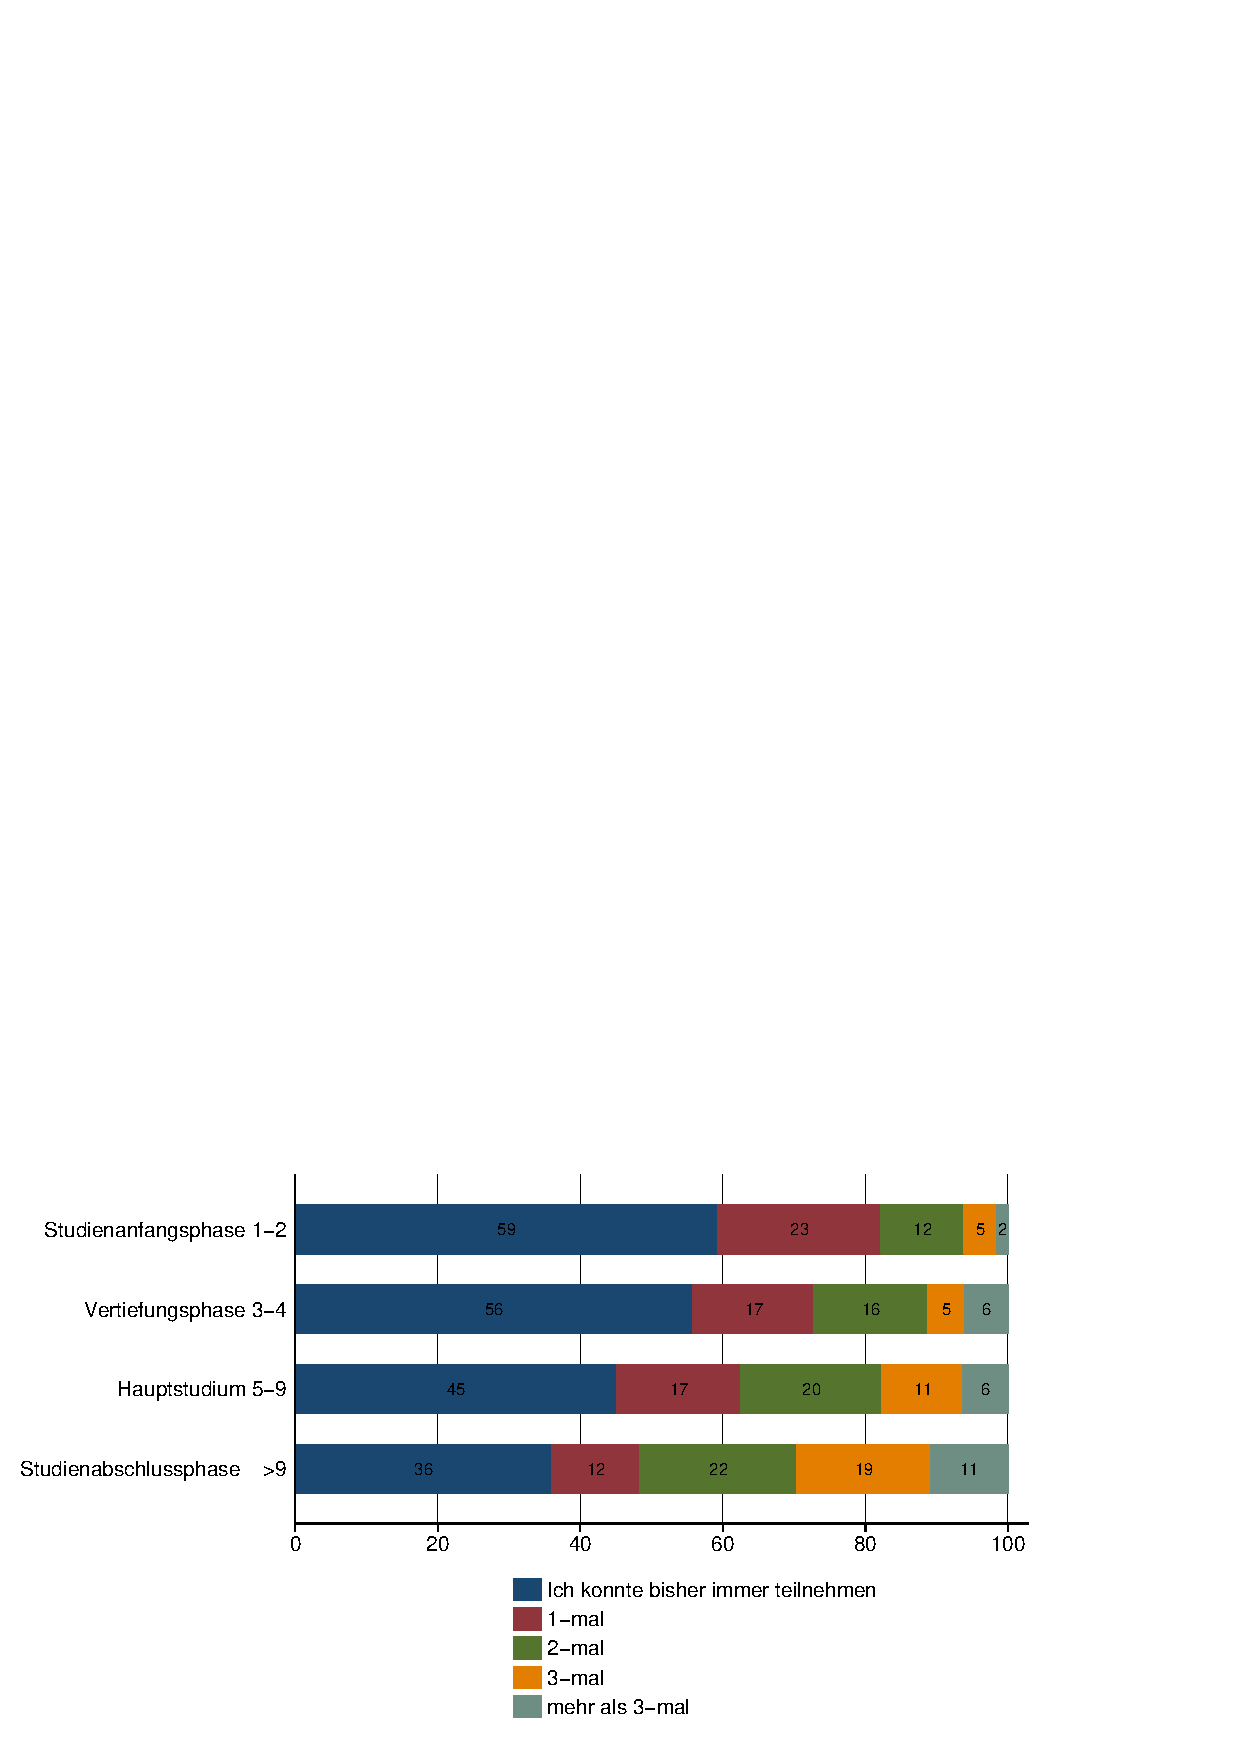
\includegraphics{image.jpg}}
	\end{center}
\end{lstlisting}
\resultarrow
\begin{center}
	\gradientframe{\face}
\end{center}


\subsection{Frame surrounding a figure with additional space}
\begin{lstlisting}
	\begin{center}
		\gradientframe[padding=5mm]{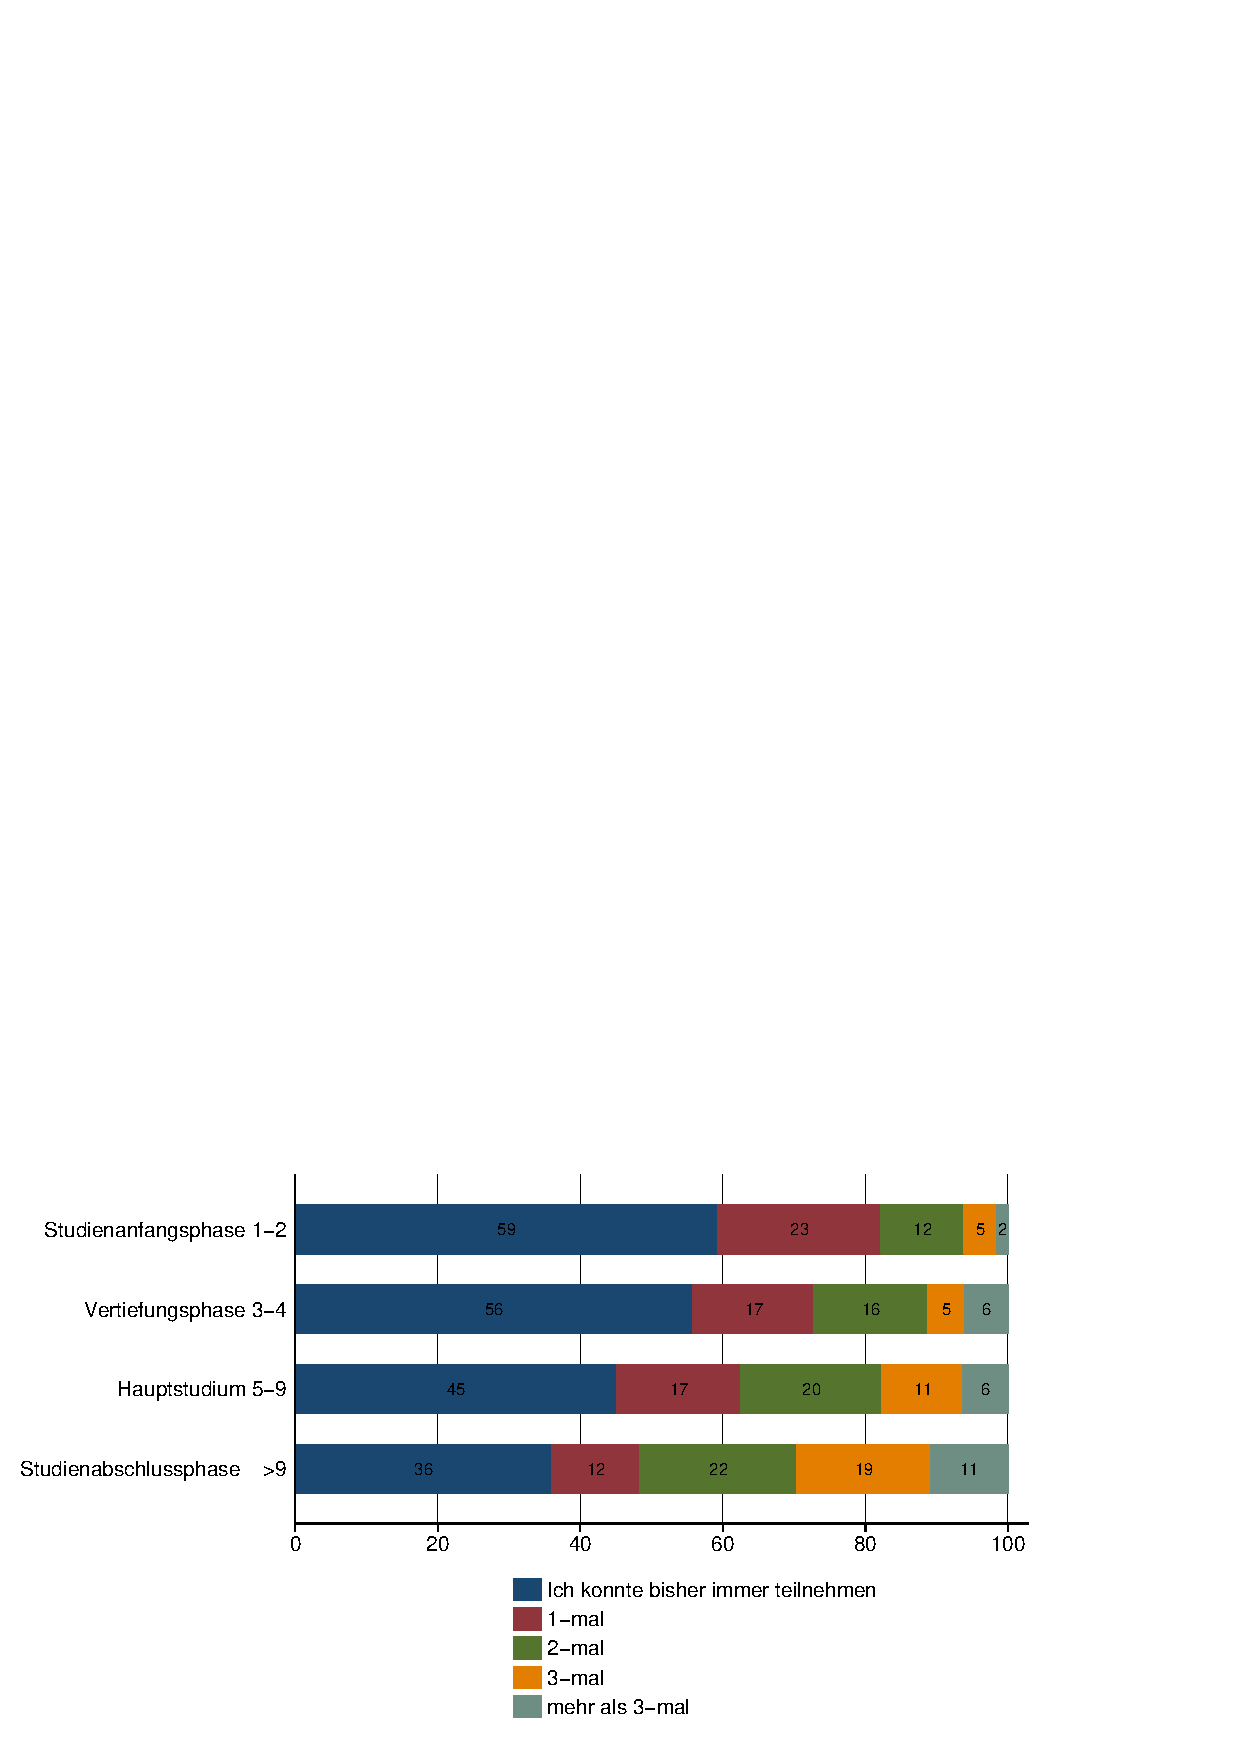
\includegraphics{image.jpg}}
	\end{center}
\end{lstlisting}
\resultarrow
\begin{center}
	\gradientframe[padding=5mm]{\face}
\end{center}


\subsection{Frame surrounding a figure with thicker frame lines and additional space}
\begin{lstlisting}
	\begin{center}
		\gradientframe[linewidth=1px,padding=5mm]{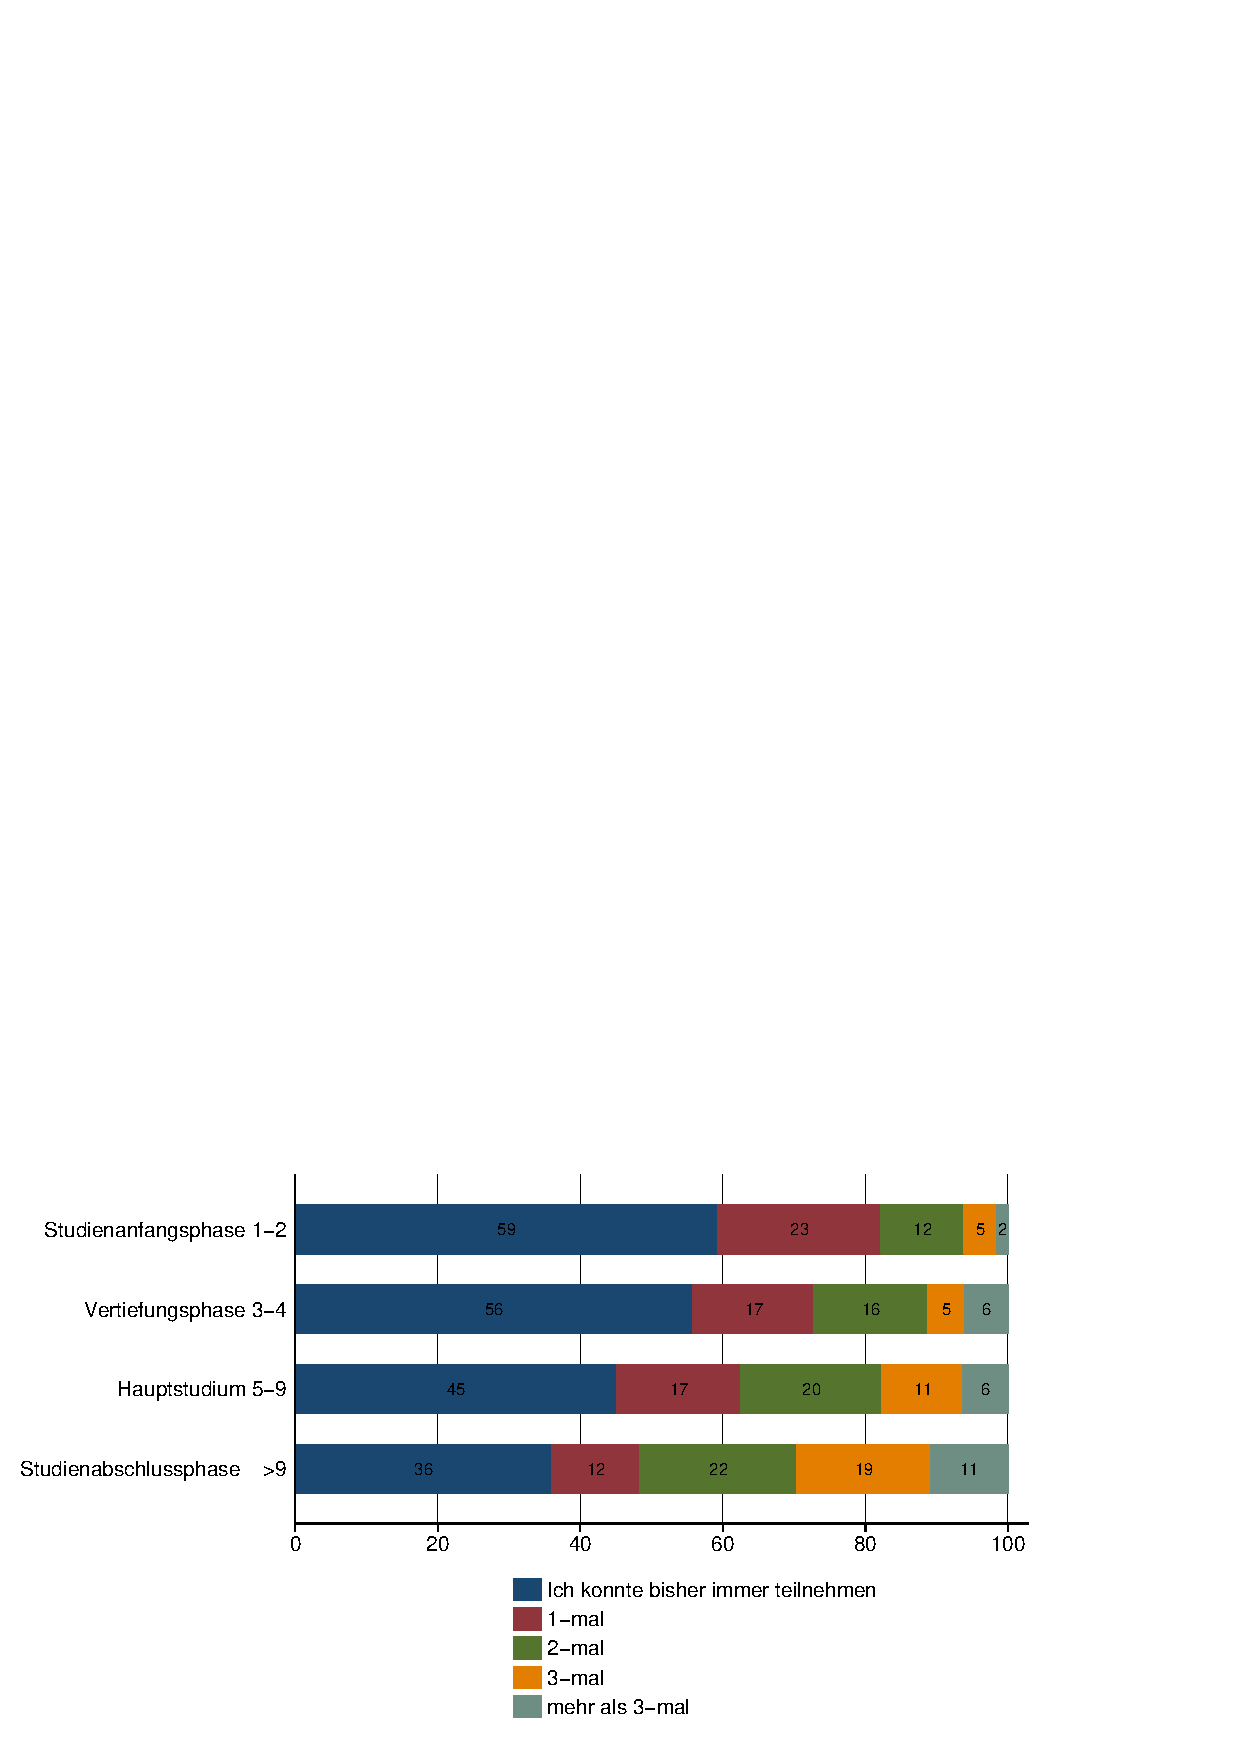
\includegraphics{image.jpg}}
	\end{center}
\end{lstlisting}
\resultarrow
\begin{center}
	\gradientframe[padding=5mm,linewidth=1px]{\face}
\end{center}


\subsection{Frame surrounding a table}
\begin{lstlisting}
	\begin{center}
		\gradientframe{%
			\begin{tabular}{r|l}
				\textbf{column A}	& \textbf{column B}	\\\hline
				cell 1A				& cell 1B			\\\hline
				cell 2A				& cell 2B			\\\hline
				cell 3A				& cell 3B			\\
			\end{tabular}%
		}
	\end{center}
\end{lstlisting}
\resultarrow
\begin{center}
	\gradientframe{%
		\begin{tabular}{r|l}
			\textbf{column A}	& \textbf{column B}	\\\hline
			cell 1A				& cell 1B			\\\hline
			cell 2A				& cell 2B			\\\hline
			cell 3A				& cell 3B			\\
		\end{tabular}%
	}
\end{center}
Be careful not to produce unintentional space when breaking lines. Add comments at line endings if needed to prevent
this, as shown in lines 2 and 8. Otherwise the result will look like this:
\begin{center}
	\gradientframe{
		\begin{tabular}{r|l}
			\textbf{column A}	& \textbf{column B}	\\\hline
			cell 1A				& cell 1B			\\\hline
			cell 2A				& cell 2B			\\\hline
			cell 3A				& cell 3B			\\
		\end{tabular}
	}
\end{center}


\clearpage
\subsection{Frame surrounding a MetaPost figure}
If you want to draw a frame around a MetaPost (or in the case of this example, MetaUML) generated figure, use the
\command{empuse} command.
\begin{lstlisting}
	\begin{center}
		\begin{empfile}
			\begin{empcmds}
				input metauml;
			\end{empcmds}
			\begin{empdef}[unique_name](0,0)
				save start, end;
				Begin.start;
				End.end;
				leftToRight(15)(start, end);
				drawObjects(start, end);
				clink(transition)(start, end);
			\end{empdef}
			\gradientframe[padding=5mm]{\empuse{unique_name}}
		\end{empfile}
	\end{center}
\end{lstlisting}
\resultarrow
\begin{center}
	\begin{empfile}
		\begin{empcmds}
			input metauml;
		\end{empcmds}
		\begin{empdef}[unique_name](0,0)
			save start, end;
			Begin.start;
			End.end;
			leftToRight(15)(start, end);
			drawObjects(start, end);
			clink(transition)(start, end);
		\end{empdef}
		\gradientframe[padding=5mm]{\empuse{unique_name}}
	\end{empfile}
\end{center}
Alternatively, you could outsource both, the \texttt{empdef} environment and the \command{empuse} command to a separate
file, and use \command{input\marg{filename}} as argument to the \command{gradientframe} command.


\section{Known issues}
\DescribeMacro\pagecolor
When using a page color different than white in combination with a (partially) transparent object, the transparent area
inside the frame will be white. To avoid this, a \command{colorbox} has to be drawn around the object. So instead of
\begin{quote}
	\command{pagecolor\marg{color}}\\
	\command{gradientframe\marg{object}}
\end{quote}
one should use
\begin{quote}
	\command{pagecolor\marg{color}}\\
	\command{gradientframe\{\command{colorbox}\marg{color}\marg{object}\}}
\end{quote}
This issue will hopefully be addressed in a future version.


\StopEventually{
	\typeout{****************************************************}
	\typeout{* To finish the installation, you have to move the}
	\typeout{* following file into a directory searched by TeX:}
	\typeout{*}
	\typeout{* \space\space \jobname.sty}
	\typeout{*}
	\typeout{* Documentation is in \jobname.\ifpdf pdf\else dvi\fi.}
	\typeout{*}
	\typeout{* Happy TeXing!}
	\typeout{****************************************************}
	\end{document}
}


\clearpage
\DocInput{\jobname.dtx}


\clearpage
%\phantomsection
%\addcontentsline{toc}{section}{Change history}
%\PrintChanges
\section{Change history}

\newlength{\notewidth}
\settowidth{\notewidth}{Note: }
\newcommand{\noteindent}{\hspace*{\notewidth}}
\begin{tabularx}{\textwidth}{|l|l|X|}
	\hline
	v0.1	& 2011/02/10	&	Initial version.
	\\\hline
	v0.1a	& 2011/02/10	&	Changed file encoding to ISO-8859-1 due to issues on CTAN.
	\\\hline
	v0.2	& 2011/02/13	&	Applied several code improvements.\newline
								Added key/value options for more flexibility.\newline
								Note: This breaks backward compatibility, so change calls in the form\newline
								\noteindent \command{gradientframe[\meta{width}]\marg{object}}\newline
								\noteindent to\newline
								\noteindent \command{gradientframe[padding=\meta{width}]\marg{object}}\newline
								\noteindent in case of an update from previous versions.
	\\\hline
\end{tabularx}


%\phantomsection
%\addcontentsline{toc}{section}{Index}
%\PrintIndex


\Finale
%</batchfile>
% \fi
%
% \section{Implementation}
%
%
% \subsection{Package header}
%	\begin{macrocode}
\NeedsTeXFormat{LaTeX2e}[1999/12/01]
\ProvidesPackage{gradientframe}[2011/02/13 v0.2 simple gradient frames around objects]
\RequirePackage{color}
\RequirePackage{keyval}
%    \end{macrocode}%^^A must be exactly 4 spaces
%
% \subsection{Options for the \command{gradientframe} command}
% The \package{keyval} package is used to handle options given to the \command{gradientframe} command by name. These
% options are:
% \begin{itemize}
%	\item \texttt{linewidth} -- defines each color's line width
%	\begin{macrocode}
\define@key{gradientframe}{linewidth}{%
	\newdimen\gradientframe@linewidth%
	\setlength{\gradientframe@linewidth}{#1}%
}%
%    \end{macrocode}%^^A must be exactly 4 spaces
%
%	\item \texttt{padding} -- defines space between the object and the innermost frame line
%	\begin{macrocode}
\define@key{gradientframe}{padding}{%
	\newdimen\gradientframe@padding%
	\setlength{\gradientframe@padding}{#1}%
}%
%    \end{macrocode}%^^A must be exactly 4 spaces
% \end{itemize}
%
%^^A \define@key{gradientframe}{outercolor}{}
%^^A \define@key{gradientframe}{innercolor}{}
%
% \begin{macro}{\gradientframe@defaults}
% The default values for these options are defined as follows:
%	\begin{macrocode}
\newcommand{\gradientframe@defaults}{%
	\setkeys{gradientframe}{%
		linewidth=0.3px,%
		padding=0mm%
	}%
}%
%    \end{macrocode}%^^A must be exactly 4 spaces
% \end{macro}
%
% \subsection{Commands}
% \begin{macro}{\gradientframe@origlinewidth}
% This dimension is used internally to preserve the original line width defined by \command{fboxrule}.
%	\begin{macrocode}
\newdimen\gradientframe@origlinewidth%
%    \end{macrocode}%^^A must be exactly 4 spaces
% \end{macro}
%
% \begin{macro}{\gradientframe@drawbox}
% This command uses two colors, for border and background, and draws one frame line.
%	\begin{macrocode}
\newcommand{\gradientframe@drawbox}[3]{%
	\fcolorbox[gray]{#1}{#2}{%
		#3%
	}%
}%
%    \end{macrocode}%^^A must be exactly 4 spaces
% \end{macro}
%
% \begin{macro}{\gradientframe}
% This command draws the grayscale gradient frame around objects. This is achieved by drawing multiple frame lines side
% by side, each with a slightly different color.
%	\begin{macrocode}
\newcommand{\gradientframe}[2][]{%
	\gradientframe@defaults% apply defaults
	\setkeys{gradientframe}{#1}%
%
	\begingroup% limit redefinitions to this block
		% backup original \fboxrule value
		\setlength{\gradientframe@origlinewidth}{\fboxrule}%
%
		\setlength{\fboxrule}{\gradientframe@linewidth}%
		\setlength{\fboxsep}{\gradientframe@linewidth}% space between frame and object
		\gradientframe@drawbox{.98}{.96}{%
			\gradientframe@drawbox{.94}{.92}{%
				\gradientframe@drawbox{.90}{.88}{%
					\gradientframe@drawbox{.86}{.84}{%
						\gradientframe@drawbox{.82}{.80}{%
							\gradientframe@drawbox{.78}{.76}{%
								\gradientframe@drawbox{.74}{.72}{%
									\setlength{\fboxrule}{\gradientframe@origlinewidth}% restore original \fboxrule value
									\setlength{\fboxsep}{\gradientframe@padding}%
									\gradientframe@drawbox{.70}{1}{#2}%
								}%
							}%
						}%
					}%
				}%
			}%
		}%
	\endgroup%
}%
%    \end{macrocode}%^^A must be exactly 4 spaces
% \end{macro}
%
\endinput
% \endinput
